\documentclass{article}

\usepackage{hyperref}
\usepackage[fleqn]{amsmath}
\usepackage{graphicx}
\usepackage{color}
\usepackage{xspace}
\usepackage{cite}
\usepackage[margin=1in]{geometry}
\usepackage{amsfonts}
\usepackage{array,multirow}
\usepackage{amssymb,amsthm}
\usepackage[]{algorithmicx}
\usepackage{algpseudocode} 
\usepackage{enumitem}
\usepackage{longtable}
\usepackage[capitalise,nameinlink,noabbrev]{cleveref}
\usepackage{float}
\usepackage{mathtools}
\usepackage{gobble}
\floatstyle{ruled}
\newfloat{algorithm}{thp}{lop}
\floatname{algorithm}{Algorithm}


\newcounter{assumptioncounter}
\newenvironment{assumption}[1][]{\refstepcounter{assumptioncounter}\par\medskip
\textbf{Assumption \theassumptioncounter} \rmfamily \itshape}{\medskip}

\newcounter{criteriacounter}
\newenvironment{criteria}[1][]{\refstepcounter{criteriacounter}\par\medskip
\textbf{Criteria \thecriteriacounter} \rmfamily \itshape}{\medskip}



\usepackage{framed}
\newenvironment{comment}
  {\par\medskip
   \color{red}%
   \begin{framed}
   \textbf{Comment: }\ignorespaces}
 {\end{framed}
  \medskip}
  
  
  

\crefname{criteriacounter}{Criteria}{criteria}
\crefname{assumptioncounter}{Assumption}{assumption}
\crefname{equation}{}{equations}


%============================

\newtheorem{theorem}{Theorem}[section]
\newtheorem{corollary}[theorem]{Corollary}
\newtheorem{definition}[theorem]{Definition}
\newtheorem{lemma}[theorem]{Lemma}
\newtheoremstyle{case}{}{}{}{}{}{:}{ }{}
\theoremstyle{case}
\newtheorem{case}{Case}
\numberwithin{theorem}{subsection}

\DeclareMathOperator*{\argmin}{arg\,min}
\DeclareMathOperator*{\argmax}{arg\,max}

\newcommand{\symboldefinition}[4]{#1}


\newcommand{\ehuffo}{{\epsilon_{\textrm{huff, 1}}}}
\newcommand{\ehufft}{{\epsilon_{\textrm{huff, 2}}}}
\newcommand{\mhufft}{{M_{\textrm{huff, 2}}}}



\newcommand{\activeconstraintsk}{{\mathbb A_{k}}}
\newcommand{\activeconstraintsl}{{\mathbb A_{l}}}
\newcommand{\activeconstraintskpo}{{\mathbb A_{k+1}}}

\newcommand{\atr}{A^{\infty}}
\newcommand{\btr}{b^{\infty}}

\newcommand{\bpr}{{B_{\infty}\left(p, r\right)}}
\newcommand{\bs}{{\beta^{(\star, k)}}}
\newcommand{\bsk}{{\beta_0^{(\star, k)}}}
\newcommand{\capcones}{{C^{(k)}_{\cap}}}
\newcommand{\chik}{{\chi^{(k)}}}
\newcommand{\chil}{{\chi^{(l)}}}
\newcommand{\ck}{{c^{(k)}}}
\newcommand{\dacc}{{\Delta_{\textrm{acc}}}}
\newcommand{\dacco}{{\Delta_{\textrm{a}}}}
\newcommand{\deltalargzik}{{\Delta_{\alpha,\beta}}}
\newcommand{\dfeas}{{\Delta_{\textrm{feasible}}}}
\newcommand{\dk}{\Delta_k}
\newcommand{\dl}{\Delta_l}
\newcommand{\dkpo}{\Delta_{k+1}}
\newcommand{\dsr}{{\Delta_{\textrm{sr}}}}
\newcommand{\fcki}{{C^{(k+1)}_{\textrm{in}}}}
\newcommand{\feasiblek}{{\mathcal F_m^{(k)}}}
\newcommand{\feasiblel}{{\mathcal F_m^{(l)}}}
\newcommand{\feasible}{{\mathcal F}}
\newcommand{\fmin}{f_{\text{min}}}
\newcommand{\gammabi}{\gamma_{\textrm{suff}}}
\newcommand{\gammasm}{\gamma_{\textrm{min}}}
\newcommand{\gcik}{{\nabla c_i \left(\xk\right)}}
\newcommand{\gk}{{\nabla m_f^{(k)}\left(\xk\right)}}
\newcommand{\gl}{{\nabla m_f^{(l)}\left(\xl\right)}}
\newcommand{\gmcik}{{\nabla m_{c_i}^{(k)}\left(\xk\right)}}
\newcommand{\gmcil}{{\nabla m_{c_i}^{(l)}\left(\xl\right)}}
\newcommand{\gradf}{\nabla f}
\newcommand{\hgik}{{\frac{\nabla m^{(k)}_{c_i}(\xk)}{\|\nabla m^{(k)}_{c_i}\left(\xk\right)\|}}}
\newcommand{\hk}{{\nabla^2m_f^{(k)}\left(\xk\right)}}
\newcommand{\huff}{{\Gamma_0}}
\newcommand{\huk}{{{\hat u}^{(k)}}}
\newcommand{\lipgrad}{{L_{\nabla}}}
\newcommand{\liphess}{{L_{\nabla^2}}}
\newcommand{\maxgrad}{{M_{\nabla}}}
\newcommand{\maxhessian}{{M_{\nabla^2}}}
\newcommand{\maxmodelhessian}{{M_{\nabla^2 m}}}
\newcommand{\maxnorm}{{M_{\|\cdot\|}}}
\newcommand{\mcik}{{{m}^{(k)}_{c_i}}}
\newcommand{\mcil}{{{m}^{(l)}_{c_i}}}
\newcommand{\mck}{{{m}_{c}}^{(k)}}
\newcommand{\mfk}{{{m}_f}^{(k)}}
\newcommand{\mfkmo}{{{m}_f}^{(k-1)}}
\newcommand{\minactivegraddelta}{{\Delta_{\mathcal A}}}
\newcommand{\minactivegrad}{{ g_{\mathcal A} }}
\newcommand{\minanglealpha}{{ \alpha^{\star} }}
\newcommand{\minangledelta}{{\Delta_{\alpha^{\star}}}}
\newcommand{\mingraddelta}{{\Delta_{\nabla c}}}
\newcommand{\mingradepsilon}{{\epsilon_{\nabla c}}}
\newcommand{\mingrad}{{ g_{\textrm{low}} }}
\newcommand{\naturals}{\mathbb N}
\newcommand{\oalpha}{\tau_{\Delta}}
\newcommand{\omegadec}{\omega_{\text{dec}}}
\newcommand{\omegainc}{\omega_{\text{inc}}}
\newcommand{\outertrk}{{T_{\text{out}}^{(k)}}}
\newcommand{\outertrkpo}{{T_{\text{out}}^{(k+1)}}}
\newcommand{\polydn}{\mathcal{P}^d_n}
\newcommand{\qk}{{Q^{(k)}}}
\newcommand{\reals}{\mathbb R}
\newcommand{\rk}{\rho_k}
\newcommand{\Rm}{\mathbb R^m}
\newcommand{\Rn}{\mathbb R^n}
\newcommand{\rotk}{{R^{(k+1)}}}
\newcommand{\sampletrk}{{T_{\text{interp}}^{(k)}}}
\newcommand{\sampletrkpo}{{T_{\text{interp}}^{(k+1)}}}
\newcommand{\scaledunshiftedellipsoid}{{{\mathcal {\hat E}_{\text{feasible}}}^k}}
\newcommand{\sdk}{{\delta_k}}
\newcommand{\searchtrk}{{T_{\text{search}}^{(k)}}}
\newcommand{\sigmamax}{{\sigma_{\textrm{max}}}}
\newcommand{\sk}{{{s}^{(k)}}}
\newcommand{\thetamink}{{\pi^k_{\textrm{min}}}}
\newcommand{\tolcrit}{\tau_{\xi}}
\newcommand{\tolrad}{\tau_{\Delta}}
\newcommand{\tr}{{ B_{\infty}\left(\xk, \dk\right) }}
\newcommand{\trkpo}{{ B_{\infty}\left(\xkpo, \dkpo\right) }}
\newcommand{\trsinfset}{{E_\textrm{infeasible}}}
\newcommand{\trstol}{{\delta_\textrm{infeasible}}}
\newcommand{\unshiftedellipsoid}{{\mathcal E^k_{\textrm{feasible}}}}
\newcommand{\wik}{{w^{(i, k)}}}
\newcommand{\ximin}{\xi_{\text{min}}}
\newcommand{\xkpo}{{{x}^{(k+1)}}}
\newcommand{\xk}{x^{(k)}}
\newcommand{\xl}{{x^{(l)}}}
\newcommand{\xinit}{{x^{(0)}}}
\newcommand{\zik}{{z^{(i, k)}}}
\newcommand{\zil}{{z^{(i, l)}}}
\newcommand{\deltamingrad}{{\Delta_{\textrm{mm}}}}
\newcommand{\mingradmodel}{{ g_{\textrm{mm}} }}
\newcommand{\activefeasiblek}{{\mathcal F^{(k)}_A}}
\newcommand{\activechik}{{\chi_A^{(k)}}}
\newcommand{\qkmo}{{Q^{(k-1)}}}
\newcommand{\qkpo}{{Q^{(k+1)}}}
\newcommand{\ckmo}{{c^{(k-1)}}}
\newcommand{\ckpo}{{c^{(k+1)}}}
\newcommand{\sdkmo}{{\delta_{k-1}}}
\newcommand{\sdkpo}{{\delta_{k+1}}}
\newcommand{\projk}{{p^{(k)}}}
\newcommand{\projl}{{p^{(l)}}}
\newcommand{\projkl}{{p^{(k,l)}}}
\newcommand{\projlk}{{p^{(l,k)}}}
\newcommand{\projkk}{{p^{(k,k)}}}
\newcommand{\projll}{{p^{(l,l)}}}
\newcommand{\trueprojk}{{p_c^{(k)}}}
\newcommand{\truefeasiblek}{{F_c^{(k)}}}
\newcommand{\truefeasible}{{F_c}}
\newcommand{\trueactiveprojk}{{\mathbb P_c^{(k)}}}
\newcommand{\nearlyactiveprojk}{{\mathbb P_{a}}}
\newcommand{\activeprojkk}{{\mathbb P^{(k, k)}}}
\newcommand{\activeprojkl}{{\mathbb P^{(k, l)}}}
\newcommand{\activeprojlk}{{\mathbb P^{(l, k)}}}
\newcommand{\activeprojll}{{\mathbb P^{(l, l)}}}
\newcommand{\unshiftedellipsoidpo}{{\mathcal E^{k+1}_{\textrm{feasible}}}}
\newcommand{\scaledunshiftedellipsoidpo}{{{\mathcal {\hat E}_{\text{feasible}}}^{k+1}}}
\newcommand{\unshiftedellipsoidkpo}{{\mathcal E^{k+1}_{\textrm{feasible}}}}
\newcommand{\image}{{\textrm{im}}}
\newcommand{\maxmodelgrad}{{M_{\nabla m}}}
\newcommand{\minangleu}{{replace me}}
\newcommand{\minanglediralt}{{w_f}}
\newcommand{\minangledir}{{u_{f not used anymore}}}
\newcommand{\minangledirk}{{u^{(k)}_f}}
\newcommand{\minangledirl}{{u^{(l)}_f}}
\newcommand{\epsactive}{{\mathbb A_c}}
\newcommand{\epsactivemodels}{{\mathbb A_{m}}}
\newcommand{\fik}{{C^{(i, k)}}}
\newcommand{\suffiterates}{{\mathcal K_{\textrm{suff}}}}
\newcommand{\miniterates}{{\mathcal K_{\textrm{min}}}}
\newcommand{\reduceiterates}{{\mathcal K_{\textrm{sr}}}}
\newcommand{\theircnot}{{\kappa_1}}
\newcommand{\theirc}{{\kappa_2}}
\newcommand{\zikthresh}{{ K_{\textrm{a}} }}
\newcommand{\jackk}{{J^{(k)}}}
\newcommand{\jackl}{{J^{(l)}}}
\newcommand{\jackkl}{{J^{(k)}_{\activeprojkk \cup \activeprojkl}}}
\newcommand{\jaclkl}{{J^{(l)}_{\activeprojkk \cup \activeprojkl}}}
\newcommand{\jackt}{{J^{(k)}_{\activeprojkk \cup \trueactiveprojk}}}
\newcommand{\huffeps}{{\epsilon_h}}
\newcommand{\huffalpha}{{\alpha_h}}
\newcommand{\huffdir}{{u_h}}
\newcommand{\huffdirk}{{u^{(k)}_h}}
\newcommand{\activeprojk}{{\textrm{active projection k}}}
\newcommand{\activeprojl}{{active projection l}}


\newcommand{\convexdistance}{{D}}





\newcommand{\activeindicesk}{{ \mathbb I_h^{(k)} }}
\newcommand{\huffindicesk}{{ \mathbb H_h^{(k)} }}
\newcommand{\inactiveindicesk}{{ \mathbb J_h^{(k)} }}
\newcommand{\huffthreshold}{{\Delta_{\textrm{H}}}}


\newcommand{\deltalb}{{\delta_{\textrm{min}}}}


\newcommand{\minactivealpha}{{ \alpha_{\textrm{h}} }}
\newcommand{\activedirk}{{ u_{h}^{(k)} }}
\newcommand{\activegradmin}{{ g_{\textrm{h}} }}


\newcommand{\modeljack}{{ \nabla m^{(k)}_{c}\left(\xk\right) }}
\newcommand{\modeljacl}{{ \nabla m^{(l)}_{c}\left(\xl\right) }}
\newcommand{\truejack}{{ \nabla c\left(\xk\right) }}


\newcommand{\zmk}{{z_m^{(k)}}}
\newcommand{\zlk}{{z_l^{(k)}}}
\newcommand{\zck}{{z_c^{(k)}}}

\newcommand{\Amk}{{\mathbb A_m^{(k)}}}
\newcommand{\Alk}{{\mathbb A_l^{(k)}}}
\newcommand{\Ack}{{\mathbb A_c^{(k)}}}


%=======================================
% Steve's definitions for marking up
%=======================================
\usepackage[normalem]{ulem}	% For color comments

\newcommand{\new}[1]{{\color{blue}#1}}
\newcommand\hcancel[2][black]{\setbox0=\hbox{$#2$}\rlap{\raisebox{.45\ht0}{\textcolor{#1} {\rule{\wd0}{1pt}}}}#2} 
\newcommand{\replace}[2]{{\color{red}\sout{#1}\color{black}{\color{red}#2\color{black}}}} %TeX source markup.
% \newcommand{\replace}[2]{{{\color{red}#2\color{black}}}} %TeX source markup.
\newcommand{\replaceb}[2]{{\color{blue}\sout{#1}\color{black}{\color{blue}#2\color{black}}}} %TeX source markup.
\newcommand{\replacemath}[2]{{\hcancel[red]{#1}{}{\color{red}#2\color{black}}}} %TeX source markup.
% \newcommand{\replacemath}[2]{{\color{red}#2\color{black}}} %TeX source markup.
\newcommand{\replacemathb}[2]{{\hcancel[blue]{#1}{}{\color{blue}#2\color{black}}}} %TeX source markup.
\newcommand{\sbnote}[1]{\textsf{{\color{cyan}{ SCB note:}   #1} }\marginpar{{\textbf{Comment}}}}


%=========================================

\title{Derivative Free Model-Based Methods for Optimization with Partially Quantifiable Convex Constraints}
\author{Trever Hallock}

\makeatletter
\def\BState{\State\hskip-\ALG@thistlm}
\makeatother

\let\oldref\ref
\renewcommand{\ref}[1]{(\oldref{#1})}

\begin{document}

\maketitle

\begin{abstract}

We propose a model-based trust-region algorithm for constrained optimization problems with convex constraints 
in which derivatives and values at infeasible points of the objective and constraint functions are not available.
In each iteration, the objective function is approximated by an interpolation model, which is then minimized over a trust region.
To ensure feasibility of all sample points and iterates, we consider construct feasible buffering cones.
We present convergence analysis.

\end{abstract}

\newpage

\section{Table of Contents}

\tableofcontents

\newpage





% Might not be able to use the \hat x.....

% DOING.TXT
%
%
% Add discussion of convergence of iterates to bounded level sets

% consolidate kappa_ef and kappa_f
% remove latex warnings
% Add motivation for why the hoffman constant is not bounded over the entire set
% \oalpha should be removed...
% define commands for pdelta, palpha, pbeta
% remove content from future work.
% The text in the sufficient reduction theorem.
% h to ht  in figures?
% prove theorem used from steve's paper
% change the final convergence theorem to be about F

% Talk more about the contributions of this paper
% Finish proofs that are WIP

% script
% 	update the table of notation





\section{Introduction}

Derivative free optimization (DFO) refers to mathematical programs involving functions for which derivative information is not explicitly available.
Such problems arise, for example, when the functions are evaluated by simulations or by laboratory experiments.
In such applications, function evaluations are expensive, so it is sensible to invest significant computational resources to minimize the number of function evaluations.

This work is ultimately aimed at developing algorithms to solve constrained optimization problems of the form 
\begin{align*}
\begin{array}{ccl} \min_{x \in \Rn} & f(x) \\
\mbox{subject to} & c_i(x) \le 0 & 1 \le i \le m,
\end{array}
\end{align*}
where 
% $\domain$ is a subset of $\Rn$, and
$f$ and $c_i, \forall 1 \le i \le m$ are real-valued functions on $\Rn$ with at least one of these functions being a {\em black-box} function, meaning that derivatives cannot be evaluated directly.
We will let the feasible set be represented as 
\begin{align}
\feasible = \{x \in \Rn | c_i(x) \le 0 \; \forall 1 \le i \le m \}. \label{define_feasible}
\end{align}

We are interested in developing {\em model-based} trust-region algorithms for solving these problems.
Model-based methods work by constructing model functions to approximate the black box functions at each iteration.
The model functions are determined by fitting previously evaluated function values on a set of sample points.
In trust-region methods, the model-functions are used to define a trust-region subproblem whose solution determines the next iterate.
For example, the trust-region subproblem might have the form

\begin{align*}
\begin{array}{ccl} \min_{\|s\| \le \dk}
 & \mfk \left(\xk+s\right) \\
\mbox{subject to} & \mcik\left(\xk + s\right) \le 0 & 1 \le i \le m, \\
& \|s\| \le \dk \\
\end{array}
\end{align*}

where $\xk$ is the current iterate, $\mfk$ is the model function approximating $f$, 
and $\mcik$ are the model functions approximating the constraint functions $c_i, \forall 1 \le i \le m$, and $\dk$ is the radius of the trust-region.
The key differences between this problem and the original is that all functions are replaced with their model functions, and a trust region constraint has been added.
We are using the models of the constraints to approximate the feasible region during each iteration:
\begin{align}
\feasiblek = \{x \in \Rn | \mcik(x) \le 0 \; \forall 1 \le i \le m \} \label{define_feasiblek}
\end{align}
Conceptually, the model functions are ``trusted'' only within a distance $ \dk $ of the current iterate $\xk$; so the trust-region subproblem restricts the length of step $s$ to be no larger than $\dk$.
To ensure that the model functions are good approximations of the true functions over the trust region, the sample points are typically chosen to lie within, or at least near, the trust-region.


We are specifically interested in applications where some of the black box functions cannot be evaluated outside the feasible region.
As in \cite{digabel2015taxonomy}, quantifiable means the functions can be evaluated at any point in $X$ and that the values returned for the constraint functions provide meaningful information about how close the point is to a constraint boundary.
We assume that the black-box functions return meaningful numerical values \emph{only} when evaluated at feasible points.
In this case, the constraints are called {\em partially quantifiable}.   
As such, we impose the requirement that all sample points must be feasible.

An important consideration in fitting the model functions is the ``geometry'' of the sample set.
This will be discussed in more detail in \cref{geometry}, but the key point is that the relative positions of the sample points within the trust region have a significant effect on the accuracy of the model functions over the trust region.
When the geometry of the sample set is poor, it is sometimes necessary to evaluate the functions at new points within the trust region to improve the geometry of the sample set.
It is well understood how to do this for unconstrained problems; but for constrained problems with all feasible sample points, some interesting challenges must be overcome.
\color{red}
The requirement that the sample points must be feasible impacts the ``geometry" of the sample set.
In this paper we explore several strategies for choosing feasible sample points with good geometry.
In particular, we consider ellipsoidal and polyhedral trust region strategies.
\color{black}
As a first step toward developing an algorithm to solve such problems, \emph{we consider a simplified problem where all of the constraints are convex}.


\section{Background}

\subsection{Notation}

Any variables that depend on the iteration will be super-scripted by $k$.
For example, the $k$-th iterate is given by $\xk$, and the model of the objective is given by $\mfk$.
The $i$-th row of the matrix $A$ is denoted $A_i$, while the $i$-th column is denoted $A_{\bullet i}$.
Subscripts on vectors are used as an index into the vector, while vectors in a sequence of vectors use superscripts.
Matrices are denoted with capital letters.
We use $e_i$ to denote the $i$-th unit vector and $e$ to denote the vector of all ones.
%, while sets are denoted with capital italic letters.

$B_k(c; \Delta)$ is the ball of radius $\Delta$ in the $k$ norm, centered at point $c$.
$\delta_{i,j}$ is the Kronecker delta, $\delta_{i, j} = \begin{cases} 1 & \textrm{if} \; i = j \\ 0 & \textrm{if} \; i \ne j \end{cases}$.
The complement of a set $S$ is denoted as $\bar S$.
Let the condition number of a matrix $Q$ be denoted $\sigma(Q)$.
Define a point $x$ subtracted from a set $S$ as $S - x = \left\{y \in \Rn | y - s \in S\right\}$.
Set addition is $X + Y = \left\{x + y | x \in X, y \in Y\right\}$.
% For any matrix $A$, we let $A^{\dagger}$ be the Moore-Penrose inverse.
\begin{align*}
a^+ = \begin{cases} a & \textrm{if} \quad a \ge 0 \\ 0 & \textrm{otherwise} \end{cases}\\
\|x\|_{\infty} = \max_{1\le i\le n}|x_i| \quad
\|x\|_{2} = \sqrt{\sum_{i=1}^n x_i^2} \quad
\|x\|_1 = \sum_{i = 1}^n |x_i|
\end{align*}
For any $m \in \naturals$, we define $[m] = \left\{i \in \naturals | 1 \le i \le m\right\}$.

\subsection{Model-based Trust Region Methods}

We modify the following derivative free trust region algorithm.
%A set of poised points are chosen for some radius $\Delta_k>0$ about the current iterate.
The objective value and derivatives are approximated in a trust region around the current iterate to construct their model functions.
Next, this model function is minimized over the trust region and the minimum argument becomes the trial point.
The objective is evaluated at the trial point and a measure of reduction $\rho$ is computed.
If $\rho$ implies that sufficient reduction has been made and that the model approximates the function well, the trial point is accepted as the new iterate.
Otherwise, the trust region is reduced to increase model accuracy.
The algorithm terminates when both a criticality measure $\chik$ and the trust region radius $\Delta_k$ reach sufficiently small thresholds of $\tau_{\chi}$ and $\tau_{\Delta}$.


For unconstrained optimization, the algorithmic framework is described in \cref{unconstrained_dfo}.

\begin{algorithm}[H]
    \caption{Unconstrained Derivative Free Algorithm}
    \label{unconstrained_dfo}
    \begin{itemize}
        \item[\textbf{Step 0}] \textbf{(Initialization)} \\
            Initialize tolerance constants $\tau_{\chi} \ge 0$, $\tau_{\Delta} \ge 0$, starting point $\xinit$, initial radius $\Delta_0 > 0$, iteration counter $k=0$, and constants $\omegadec \in (0, 1)$, $ \gammasm \in (0, 1)$, $\gammabi \in (\gammasm, 1)$.
            
        \item[\textbf{Step 1}] \textbf{(Construct the model function)} \\
            Call the model improvement ``\cref{model_improving_algorithm}" to provide a set of sample points $Y^{(k)}$.
            Evaluate the objective on these points and use interpolation \cref{interpolation_formula} to construct the model function $\mfk(x)$.
        
        \item[\textbf{Step 2}] \textbf{(Check stopping criteria)} \\
            Compute the criticality measure $\chik$ such as $\chik = \|\nabla\mfk(\xk)\|$. \begin{itemize}
                \item[] If $ \chik < \tau_{\chi} $ and $\Delta_k<\tau_{\Delta}$ then return solution $\xk$.
                \item[] If $ \chik < \tau_{\chi} $ but $\Delta_k\ge\tau_{\Delta}$ then  
                set $\Delta_{k+1} \gets \omegadec\Delta_{k}$, 
                $x^{(k+1)} \gets \xk$,
                $k \gets k+1$ and go to Step 1.
            \end{itemize}
        
        \item[\textbf{Step 3}] \textbf{(Solve the trust region subproblem)} \\
            Compute $\sk = \argmin_{s\in B_2(0; \Delta_k)} \mfk (\xk + s)$ where $B_2(0; \Delta_k)$ is the ball of radius $\Delta_k$ defined in \cref{tab:TableOfNotation}.
            
        \item[\textbf{Step 4}] \textbf{(Test for improvement)} \\
            Compute $\rk$ with \cref{define_rhok} \begin{itemize}
                \item[] If $\rk < \gammasm$ then $\xkpo \gets \xk$ (reject) and $\Delta_{k+1} \gets \omegadec\Delta_{k}$
                \item[] If $\rk \ge \gammasm$ and $\rk < \gammabi$ then $\xkpo\gets\xk+\sk$ (accept) $\Delta_{k+1} \gets \omegadec\Delta_{k}$
                \item[] If $\rk \ge \gammabi$ and $\|\sk\| = \Delta_{k}$ then $\xkpo=\xk+\sk$ (accept) $\Delta_{k+1} \gets \omegainc\Delta_{k}$
                % and either increase the radius or decrease if $\nabla \mfk(\xk)$ is small
            \end{itemize}
            $k \gets k+1$ and go to Step 1.
    \end{itemize}
\end{algorithm}

This derivative-free optimization algorithm differs from the classical trust region algorithm in two important respects:
\begin{enumerate}
    \item Models are constructed without derivative information.
    \item The trust region radius $\Delta_k$ must go to zero as $k\to\infty$.
\end{enumerate}

This is required to ensure that the gradient of the model function is equal to the gradient of $f$ in the limit.
Our goal is to generalize this framework to handle constraints, 
where we must ensure no constraint violation occurs
\color{red}
while also ensuring the accuracy of the models of the constraints
\color{black}
.

\section{Derivative Free Background}
\subsection{Recent Work}
\paragraph{Applications}

Recently, there has been a growth in applications of derivative free optimization.
Such applications include photo-injector optimization \cite{1742-6596-874-1-012062}, circuitry arrangements \cite{PLOSKAS201816}, machine learning \cite{KS2018}, volume optimization \cite{Cheng2017}, and reliability based optimization \cite{Gao2017}.

\paragraph{Constrained derivative free algorithms}
To address the rise in these applications, new algorithms are being developed such as \cite{doi:10.1080/10556788.2015.1026968} which is an algorithm similar to the one presented here, but the sample points are not always feasible.
\cite{Troltzsch2016} presents another similar algorithm for equality based constraints.
\cite{BAJAJ2018306} presents an algorithm which accepts an infeasible starting point.
\cite{Gao2018} also presents an algorithm for linearly constrained derivative free optimization that uses a backtracking technique to minimize the number of evaluations required.

\paragraph{Reviews}
Within \cite{introduction_book} derivative-free methods are developed in detail.
This is the first text book devoted to derivative free optimization.
It contains a good explanation of ensuring geometry of the current set with poisedness for unconstrained problems and also covers other derivative-free methods including direct-search and line search.

A good review of derivative free algorithms and software libraries can be found in \cite{miguel_review}.
This compares several software libraries, and reviews the development of derivative free optimization since it started.
Another recent review can be found in \cite{custodio_review2} and \cite{larson_menickelly_wild_2019}.


\subsection{Sample Set Geometry}
\subsubsection{Interpolation}
\label{interpolation}

Derivative free trust region methods construct model functions from a family of functions spanned by a set of $p + 1 \in \naturals$ basis functions  $\{\phi_0, \phi_1, \ldots, \phi_p\}$.
Each member of this family has the from $\mfk(x) = \sum_{i=0}^p\alpha_i\phi_i(x)$ for some scalar coefficients $\alpha_i, i \in \{0, \ldots, p\}$.

In our method, we use interpolation to choose the coefficients so that $\mfk$ agrees with $f$ on a set of $p+1$ sample points $Y = \{y^0, y^1, \ldots, y^p\}$ for which the functions have been evaluated.
Thus the model functions must satisfy:
\begin{align}
\label{interpolation_condition}
\mfk(y^i) = f(y^i) \quad \forall \quad 0 \le i \le p.
\end{align}
This is known as the \emph{interpolation condition}.

To satisfy the interpolation condition \cref{interpolation_condition}, we chose the linear combination by selecting coefficients $\alpha_0, \ldots, \alpha_p$ to satisfy
\begin{align}
\label{interpolation_formula}
    \mfk(y^i) = \sum^p_{j=0}\alpha_j\phi_j(y^i) = f(y^i) \quad \forall \quad 0 \le i \le p.
\end{align}

% We can also write this equation in matrix form.
If we define the Vandermode matrix as
\begin{align}
\label{vandermonde}
V=
\begin{pmatrix}
    \phi_0(y^0)      & \phi_1(y^0)       & \ldots & \phi_{p}(y^0)      \\
    \phi_0(y^1)      & \phi_1(y^1)       & \dots  & \phi_{p}(y^1)      \\
                     &                   & \vdots &                    \\
    \phi_0(y^{p})    & \phi_1(y^{p})     & \ldots & \phi_{p}(y^{p})
\end{pmatrix},
\end{align}

the interpolation condition becomes:
\begin{align}
\label{matrix_form}
V
\begin{pmatrix}
    \alpha_0     \\
    \alpha_1     \\
    \vdots       \\
    \alpha_p
\end{pmatrix}
=
\begin{pmatrix}
    f(y^0)     \\
    f(y^1)     \\
    \vdots     \\
    f(y^p)
\end{pmatrix}
\end{align}

% Suppose that we use $p+1$ sample points $Y = \{y^0, y^1, \ldots, y^p\}$ to construct the approximation of $f$.
We desire a method for choosing these sample points that provides error bounds on both 
the function values and orders of derivatives in some region around the current iterate.
% The model is constructed to agree with the original functions on at least the sample points: we evaluate the objective here, so that we know the true function values at these points.
% For the objective, this becomes

%It is convenient to write the model as a linear combination of basis polynomials $\{\phi_0, \phi_2, \ldots, \phi_p\}$.


\subsubsection{Geometry}
\label{geometry}
The term \emph{geometry} describes how the distribution of points in the sample set $Y$ affects the model's accuracy.
\cref{matrix_form} has a unique solution if and only if $V$ is nonsingular, in this case, we say that the sample set $Y$ is \emph{poised} for interpolation with respect to the basis functions $\phi_i$.
However, even when $V$ is nonsingular but ``close" to singular, as measured by its condition number, the model's approximation may become inaccurate.
% The condition number of $V$ measures how far the current Vandermode matrix is from being illpoised.
Algorithms must be careful to avoid choices of sample points $Y$ that cause the condition number of this matrix to be too large.

In the case of polynomial model functions, a careful analysis of model accuracy can be performed using \emph{Lagrange polynomials}.
Let the space of polynomials with degree less than or equal to $d$ be denoted $\polydn$ and have dimension $p+1$.
The Lagrange polynomials $l_0, l_1, \ldots, l_p$ for the sample set $Y$ are a basis of $\polydn$ such that
\begin{align*}
l_i(y^j) = \delta_{i,j}
\end{align*}
where $\delta_{i,j} = \{0 \;\text{if}\; i\ne j,\quad 1 \;\text{if} \; i = j \}$ is the Kronecker-delta function.
%For example, after this change of basis, note that the Vandermonde matrix becomes the identity matrix.
Thus, we can conveniently write
\begin{align}
\label{reg}
\mfk(x) = \sum^p_{j=0}f(y^i)l_i(x).
\end{align}
%This implies computing the change of basis to the Lagrange polynomials amounts to inverting this Vandermonde matrix.
%This relationship allows us to use properties of the Vandermonde matrix and these Lagrange polynomials to find conditions on our sample points that ensure nice geometry.

We say that a set $Y$ is \emph{$\Lambda$-poised} for a fixed constant $\Lambda$ with respect to a bases $\phi$ on the set 
$B \subset\Rn$ if and only if for the Lagrange polynomials $l_i$ associated with $Y$ satisfy
\begin{align}
\Lambda \ge \max_{0\le i\le p}\max_{x\in B}|l_i(x)|.
\end{align}

% This can be shown to be equivalent to the following condition \cite{introduction_book}.
% For any $x \in B_2(0, 1)$ there is a $\lambda \in \reals ^ {p+1}$ such that 
% \begin{align}
% \sum_{i=0}^p\lambda_i\phi_i(y^i) = \phi(x) \\
% \|\lambda\|_{\infty} \le \Lambda.
% \end{align}

% This can ensure that the Vandermonde matrix is well conditioned.
This is useful because of \cref{quadratic_errors}, which is shown in \cite{introduction_book}.

\begin{theorem}
\label{quadratic_errors}
Assume that $Y = \{y^0, y^1, \ldots, y^p\} \subset \Rn$ with $p_1 = p+1= \frac{(n+1)(n+2)}{2}$ is a $\Lambda$
poised set of sample points for quadratic interpolation contained in the ball $B(y^0; \Delta_Y)$ of radius $\Delta_Y = \max_{i \in [p]} \|y^0 - y^i\|$.
Further, assume that the function $f$ is twice continuously differentiable in an open domain $\Sigma$ containing $B(y^0; \Delta_Y)$ and $\nabla^2 f$
is Lipschitz continuous in $\Omega$ with constant $L_h > 0$.

Then, if $m$ is a quadratic model function for $f$ constructed as in \cref{reg}, there exist constants $\kappa_f$, $\kappa_g$, $\kappa_h$ dependent only on $p_1$, $L_h$, and $\Lambda$ such that:
\begin{align}
\|\nabla^2 f(y) - \nabla^2 m(y)\| \le \kappa_{h} \Delta \quad \forall y \in B_2(y^0; \Delta_Y) \label{error_in_hessian}\\
\|\gradf(y) - \nabla m(y)\| \le \kappa_{g} \Delta^2 \quad \forall y \in B_2(y^0; \Delta_Y) \label{error_in_gradient} \\
|f(y) - m(y) | \le \kappa_{f} \Delta^3 \quad \forall y \in B_2(y^0; \Delta_Y). \label{error_in_function} 
\end{align}
\end{theorem}


Also, \cite{introduction_book} also shows that ensuring a bound on the condition number of the Vandermonde matrix ensures $\Lambda$-poisedness.
In particular, these bounds ensure that the following accuracy condition is satisfied, which we can adapt a proof from \cite{Conejo:2013:GCT:2620806.2621814} to prove convergence to a first order critical point: 
\begin{align}
\label{accuracy}
\|\nabla \mfk(\xk) - \gradf(\xk) \| \le \kappa_g \dk^2
\end{align}
for some fixed constant $\kappa_g$ independent of $k$.
This will need accuracy for both the objective and the constraints, as described in \cref{accuracy_is_satisfied}
We have extend these results for ellipsoidal trust regions in \cref{ellipsoidal_lambda}.
 
A more detailed discussion can be found in \cite{doi:10.1080/10556780802409296}, but a step to ensure good geometry is required for convergence analysis although it may come at the expense of adding more function evaluations.

\subsubsection{Geometry Ensuring Algorithms}

Sample points are chosen by a geometry ensuring algorithm from \cite{introduction_book}.
At any given time, the algorithm has evaluated 1 or more sample points.
Initially, only the starting point $x_0$ is evaluated, so that points must be added to the sample set.
Evaluated points within the trust region should be reused when possible, but the algorithm may have to replace some points to ensure a well poised set on the new trust region.
We call the algorithm that adds points, replacing where necessary, the \emph{model improvement algorithm}.
One classic such algorithm is presented in \cite{introduction_book}.

The idea behind this algorithm is to perform an LU factorization with partial pivoting on the Vandermonde matrix.
As we have seen, this computes the basis for the Lagrange polynomials corresponding to $Y$.
However, when this LU factorization encounters a small pivot, the point corresponding to that row is replaced, improving the condition number of the Vandermonde matrix.

In practice, we first shift the sample set $Y$ by subtracting the current iterate and dividing by the trust region radius:
\begin{align}
\bar{Y} = [0, \frac{y^1 - y^0}{\Delta}, \ldots, \frac{y^p - y^0}{\Delta}]
\end{align}

At times, the algorithm will not have all $p+1$ points.
This can be because it is only given one point during initialization, or because points not within the trust region are removed.
Because the model improvement algorithm requires all $p+1$ points, we initialize $y^i = y^0$ for any $0 < i \le p$ corresponding to a missing point.
We choose a threshold 
\begin{align}
0 < \ximin < 1 \label{define_ximin},
\end{align} and follow \cref{model_improving_algorithm}:

\begin{algorithm}[H]
    \caption{Model Improvement Algorithm}
    \label{model_improving_algorithm}
    \begin{itemize}
        \item[\textbf{Step 0}] \textbf{(Initialization)} \\
            Initialize $i=1$.
            Given a non-empty set $Y$ of $p+1$ points. 
            Construct the Vandermonde matrix $V_{i,j} = \phi_j(\frac 1 {\Delta}(y^i - y^0))$.
			Initialize constant $\ximin > 0$.
        \item[\textbf{Step 1}] \textbf{(Pivot)} \\
            Swap row $i$ with row $i_{\max} = \arg \max_{j|j\ge i} V_{j,i} $
        
        \item[\textbf{Step 2}] \textbf{(Check threshold)} \begin{itemize}
                \item[] If $|V_{i,i}| < \ximin$ then select \label{next_point} $\hat y \in \argmax_{t | \|t\|\le 1} |\phi_i(t)|$
                \item[] Replace row $i$ with $V_{i, j} \gets \phi_j(\hat y)$.
                \item[] $Y \gets Y \cup \{\hat y \}\\ \{y^i\}$
            \end{itemize}
        
        \item[\textbf{Step 3}] \textbf{(LU)} \begin{itemize}
%                 \item[] Set $V_i \gets \frac{1}{V_{i,i}} V_i$
                \item[] Set $V_{\bullet j} \gets V_{\bullet j} - \frac{V_{i,j}}{V_{i, i}} V_{\bullet j} \forall j=i \ldots p$
            \end{itemize}
            If $i = p$ then \textbf{Stop}, otherwise Set $i \gets i+1$ and go to Step 1
    \end{itemize}
\end{algorithm}


% At the end of this algorithm, the points in $Y$ will be $\Lambda$-poised for some $\Lambda$ depending on the constant $\xi_{min}$.
The following result is shown in \cite{introduction_book} through Theorem 6.5, Theorem 3.14, and 6.7 Exercise 3.
\begin{theorem}
\label{set_is_poised}
After running \cref{model_improving_algorithm}, the resulting set $Y$ is Lambda poised for some $\Lambda > 0$ that depends on $\xi_{\text{min}}$.
\end{theorem}

This algorithm can also be used to create a poised set over an ellipsoidal shape.
This is discussed further in \cref{ellipsoidal_lambda}.



\subsection{Algorithm Components}

Before describing the algorithm, we discuss several referenced components.

\subsubsection{Criticality Measure}

In order to define stopping criteria for the algorithm, we introduce a criticality measure $\chi$ which goes to zero as the iterates approach a first order critical point.
When the criticality measure is small, we must also decrease the trust region radius.
Once this has reached a small enough threshold $\tau_{\chi}$ and the trust region is small enough ($\Delta_k < \tau_{\Delta}$), we can terminate the algorithm.
For now, our algorithm is designed to work with convex constraints, so we employ a classic criticality measure discussed in \cite{ConnGoulToin00} of
\begin{align}
\label{define_criticality_measure}
\chik = \left\|\xk - \text{Proj}_{\feasiblek}\left(\xk- \nabla \mfk\left(\xk\right)\right)\right\|.
\end{align}
Recall that $\feasiblek$ was defined by \cref{define_feasiblek}.
The first order optimality conditions for $x^{\star} \in \Rn$ to by a local optimum of $f$ is that $x^{\star}$ satisfies
\begin{align*}
x^{\star} = \text{Proj}_{\feasiblek}\left(x^{\star} - \gradf(x^{\star})\right).
\end{align*}
For convex constraints, this condition is necessary and sufficient under regularity assumptions.
Thus, our criticality measure measures how far the current iterate is from satisfying the first order optimality conditions for $\xk$ to be a optimum of $\mfk$.
In turn, as $\dk \to 0$, the model $\mfk$ better approximates $f$, $\feasiblek$ better approximates $\feasible$ and $\xk$ approaches an optimum of $f$.

In practice, we introduce constants 
\begin{align}
            \tolcrit, \tolrad \ge 0 \label{define_algorithm_tolerances}
\end{align}
that we use as thresholds to determine when the criticallity measure and trust region radius are sufficiently small.

\subsubsection{Assessing Model Accuracy and Radius Management}

Each iteration that evaluates a trial point must also test the accuracy of the model functions.
To test the accuracy, we calculate a quantity
\begin{align}
\label{define_rhok}
\rk = \frac{f(\xk) - f(\xk+\sk)}{\mfk(\xk) - \mfk(\xk+\sk)}
\end{align}
which measures the actual improvement over the predicted improvement.
A small $\rk$ implies the model functions are not sufficiently accurate.
Values of $\rk$ close to $1$ imply that the model accurately predicted the new objective value.
A large $\rk$ implies progress in minimizing the objective, although the model was not accurate.
This has been widely used within trust region frameworks such as \cite{Conn:2000:TM:357813} and within a derivative free context \cite{introduction_book}.

\begin{comment}
Steve wants me to move this...
\end{comment}
The user supplies fixed constants
\begin{align}
0 < \gammasm < \gammabi \le 1	\label{define_the_gammas}
\end{align}
as thresholds on $\rk$ and
\begin{align}
0 < \omegadec < 1 \le \omegainc		\label{define_the_omegas}
\end{align}
$\omegadec, \omegainc$ as decrement and increment factors to determine the trust region update policy.
That is, when $\rk < \gammasm$, the trust region is decreased by a factor of $\omegadec$, and when the trust region is increased by a factor of $\omegainc$
during some iterations in which $\rk > \gammabi$.

In addition to decreasing the trust region to innacurate trial steps, 
it must also be decreased when the criticallity measure is small relative to the trust region.
To accomplish this, we introduce constants
\begin{align}
0 < \kappa_{\chi} \label{define_kappa_chi} \\
0 < p_{\Delta} < \min\{p_{\alpha}, p_{\beta}\} \le 1 \label{define_p_delta} 
\end{align}
and check
\begin{align}
\kappa_{\chi} \dk^{p_{\Delta}} \le \chik \label{criticallity_check}
\end{align}
to ensure the trust region radius does not remain large while approaching criticallity.
Here,
$p_{\alpha}$ and $p_{\beta}$ is defined by \cref{define_abpab},
while $\chik$ is defined by \cref{define_criticality_measure}.


\section{Algorithm}
\label{infeasible_point_strategies}


The algorithm for convex constraints is complicated by the fact that we only have models for the constraint functions.
Errors in these models mean that we may attempt to evaluate a point that is not feasible in two ways:
\begin{itemize}
\item A point chosen by the geometry ensuring algorithm may be infeasible.
\item The trial point solving the trust region subproblem may be infeasible.
\end{itemize}


% What remains in throughout \cref{infeasible_point_strategies} is a discussion of various strategies
% for handling infeasible sample points.
To deal with these two forms of infeasible points, we have developed several strategies that make use of three separate trust regions.
These trust regions are a box-shaped outer trust region $\outertrk$,  an ellipsoidal inner trust-region $\sampletrk$ from which the sample points are chosen,  and a search trust-region, $\searchtrk$, which constrains the search for the next iterate.
The outer trust region is an $L_{\infty}$ ball of radius $ \dk $ defined by
\begin{align}
\outertrk = \tr = \{x\in \Rn | \; \xk_i - \dk \le x_i \le \xk_i + \dk \quad \forall i \in [n]\}. \label{define_outer_trust_region}
\end{align}

Note that the outer trust region may include infeasible points.
To ensure feasibility of all sample points, we construct an inner trust region  $ \sampletrk $  satisfying 
$\sampletrk \subset \outertrk \cap \feasiblek$.
Since $\feasiblek$ is only an approximation of $\feasible$,  we place additional restrictions on $\sampletrk$
to ensure that it is entirely contained within the feasible region $\feasible$.
These restrictions will be described in \cref{ellipsoid_requirements}, 
and we show that these restrictions ensure $\sampletrk \subset \feasible$ in \cref{ellipsoid_is_feasible} and \cref{searchtrk_is_feasible}.

%\cref{ellipsoid_is_feasible}

% However, we do not want to limit the search for a new iterate to the same trust region we use to construct the model.
The third trust region $\searchtrk$ is the search trust region, which could either be $\sampletrk$ itself, 
or a larger region satisfying $ \sampletrk \subset \searchtrk \subset \outertrk \cap \feasible$.
The search trust region is used in defining the trust region subproblem.

% \replace{
% Within our algorithm, if $ \outertrk \subseteq \feasible$ we can set $ \sampletrk $ to be a sphere of radius $\dk$.
% This saves the computation of $ \sampletrk $ when it is not needed, as there are no nearby constraints.}{}  \sbnote{I don't think this needs to be said here}

% In the last paper, we showed convergence of our algorithm for linear constraints.
% We follow the same pattern as in that paper, but we must deal with some problems introduced by general convex constraints.
% To avoid evaluating infeasible points with general convex constraints, we construct models of the constraints in addition to the objective.


What remains in \cref{infeasible_point_strategies} is devoted to search strategies for ensuring feasible sample points:
\cref{possible_ellipsoids} and \cref{handling_linear_constraints_within_ellipsoid_programs} could be considered background, while the others discuss algorithms.
The version we call the ``conservative ellipsoid'' is lengthier and discussed within \cref{constructing_and_analysizing_conservative_ellipsoid}.
Within \cref{convex_model_reduction} we examine two strategies for handling infeasible trial points.
Finally, in \cref{the_algroithm_section}, we state the convergent algorithm, which is based on the strategies found in 
\cref{constructing_and_analysizing_conservative_ellipsoid} and \cref{decreasing_the_trust_region_for_infeasible_trial}.



% We will show feasibility and convergence of the algorithm assuming certain of these 


% Although an approach for avoiding one of these two function evaluations can work for the other in thoery, we stick to one simplified version.

% \subsection{Implemented Ideas not used in this paper}
% 
% 
% \subsubsection{Using higher order models}
% I have implemented an algorithm that uses higher order models to approximate the constraints.
% 
% In this algorithm, we add additional degrees of freedom to the constraints to cut off points that have been evaluated and are infeasible.
% The models are forced to be a given negative value at these points.
% 
% One question for this method is how many constraints to model.
% 
% 
% I implemented Kriging, as this can use as many points as are available.
% However, this requires using some artificial value of the constraints at infeasible points.


\subsection{Constructing the Sample Region}
\label{possible_ellipsoids}

We ensure that sample points are feasible by constructing an inner trust region $\sampletrk$ that we show is feasible for small enough $\dk$.
\begin{comment}
Steve wants me to delete most of this...
\end{comment}
This means that if $\sampletrk$ includes infeasible points-and we attempt to evaluate at an infeasible point- we can reduced the trust region radius.
Of course, the method of constructing this ellipsoid impacts the algorithm's efficiency because constructing a $\sampletrk$ too small means a poor sample set,
while using a $\sampletrk$ too large implies reducing the trust region quickly so that only small steps can be made towards a critical point.

There is a well known algorithm for constructing poised sets over spheres, and this algorithm can be easily generalized to an ellipsoid.
Therefore, we construct an ellipsoidal inner trust region to avoid the constraints.


\subsubsection{Buffering Cones}
\label{ellipsoid_requirements}
% We construct a set of requirements $\sampletrk$ must satisfy.
During iteration $k$, let $\sampletrk$ be defined by a $n\times n$ symmetric, positive definite matrix $\qk$, center $\ck \in \Rn$, and radius $\delta_{k} > 0$:
\begin{align}
\sampletrk = \left \{x \in \Rn | (x - \ck)^T \qk(x - \ck) \le \frac 1 2 \sdk^2 \right \}. \label{define_sampletrk}
\end{align}
To ensure this ellipsoid is feasible, we construct cones that buffer the ellipsoid from the constraint boundaries.
These cones have a vertex between the current iterate and the nearest point along the linearization of the constraints, and open towards the current iterate.
We define these cones within this section.

The first step is to identify the set of constraints that are nearly active relative to the size of the current trust region.
Let $\zik$ denote the projection of the current iterate $\xk$ onto the hyperplane defined by the $i$-th constraint model.
Specifically, for each $i$ with either $\left\|\gmcik\right\| \ne 0$ or $c_i\left(\xk\right) = 0$, define
\begin{align}
\label{define_z}
\zik =
\begin{cases}
\xk &  c_i\left(\xk\right) = 0 \\
\xk - \frac{m^{(k)}_{c_i}\left(\xk\right)}{\left\|\gmcik\right\|^2} \gmcik & \left\|\gmcik\right\| \ne 0
\end{cases}
\end{align}
Note that this definition is consistent when both $c_i\left(\xk\right) = 0$ and $\left\|\gmcik\right\| \ne 0$.
If $\zik$ lies sufficiently near the outer trust region, we say that the $i$-th constraint is \emph{nearly active}.
Specifically, the set of nearly active constraints is defined by
\begin{align}
\activeconstraintsk = \left\{i \in [m] \bigg| \zik \in B_{\infty}\left(\xk, (1+\zikthresh)\dk\right)\right\}, \label{define_activeconstraints}
\end{align}
where $\zikthresh$ is a user defined parameter that must satisfy the following identity involving $\omegainc$ (which is defined by \cref{define_the_omegas}):
\begin{align}
(2 + \omegainc)\sqrt{n} < \zikthresh. \label{define_zikthresh}
\end{align}
For each nearly active constraint, we define a buffering cone with user defined parameters
\begin{align}
\alpha, \beta, p_{\alpha}, p_{\beta} \in (0, 1). \label{define_abpab}
\end{align}
The vertex $\wik$ of this cone is located along the line segment connecting $\xk$ to $\zik$:
\begin{align}
\wik = \xk + \left(1 - \alpha\dk^{p_{\alpha}}\right)\left(\zik - \xk\right). \label{define_w}
\end{align}
The cone for constraint $i$ is then defined by
\begin{align}
\fik = \left\{x \in \Rn | x = \wik + t s,t > 0, \|s\| = 1, -s^T\hgik \ge \beta \dk^{p_{\beta}} \right\}. \label{define_fik}
\end{align}
This cone is illustrated in \cref{explanation_2}.
\begin{figure}[ht]
    \centering
    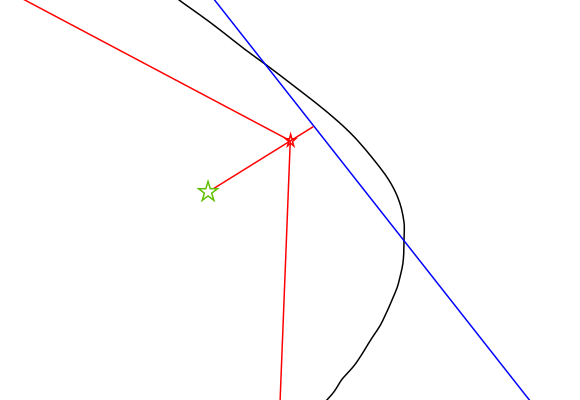
\includegraphics[width=150px]{images/explanation_2.png}
    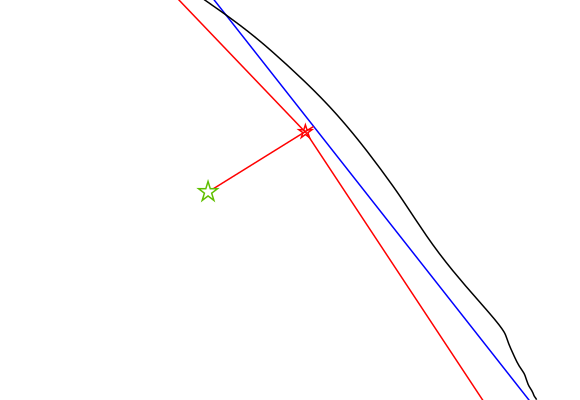
\includegraphics[width=150px]{images/explanation_3.png}
    \caption{
    	The current iterate is the green star;
    	the true constraint is black;
    	the vertex, $\wik$, is the red star;
    	the linearization of the constraint boundary is blue;
    	the cone buffering cone $\fik$ is in red.
    	As the trust region goes to zero the buffering cone better approximates the linearization of the constraint and becomes locally feasible.
	}
    \label{explanation_2}
\end{figure}
The intersection of these cones is the set
\begin{align}
\capcones = \{x\in\Rn | \; x \in \fik \quad \forall i \in \activeconstraintsk \} \label{define_capcones}
\end{align}
which is depicted in \cref{completed_2}.
In \cref{cone_and_tr_are_feasible}, we show that for sufficiently small $\dk$, $\capcones \cap \outertrkpo \subseteq \feasible$.
Therefore, to obtain feasible sample points, we require that 
\begin{align*}
\sampletrkpo \subset \capcones \cap \outertrkpo.
\end{align*}


\begin{figure}[ht]
    \centering
    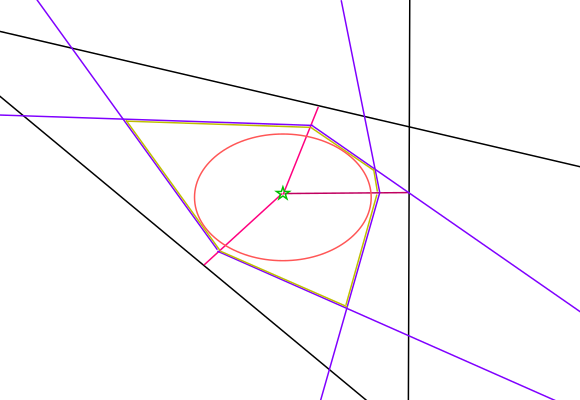
\includegraphics[width=150px]{images/completed_2.png}
    \caption{
    	After constructing 
    	the linearization of the constraints in black;
    	the buffering cones in blue;
    	the trusted region $\capcones$ in yellow;
    	we seek to find an ellipsoid within $\capcones$, such as the one in red/pink.
	}
    \label{completed_2}
\end{figure}


\subsubsection{Linear Constraints}
\label{handling_linear_constraints_within_ellipsoid_programs}

Throughout discussing strategies for constructing an ellipsoid within the buffering cones, we must also require that the ellipsoid is contained within the trust region.
Because our trust region is $\tr$, we can satisfy the trust region constraints by including linear constraints of the form $\xk_i - \dk \le x_i \le \xk_i + \dk$.
As done in the linear paper, using the work of \cite{Khachiyan1993}, we handle the general constraints $Ax \le b$ for some $m\times n$ matrix $A$ and $b \in \Rm$.
That is, given a polyhedron $P = \{ x \in \Rn\; | \;  Ax \le b \}$ defined by an $m \times n$ matrix $A$, and $b \in \Rm$,
we wish to find the maximum-volume ellipsoid $E \subset P$ centered at a point $\mu \in P$.

Let $\bar{b} = b - A\mu$ and $d = x - \mu$ so that the polyhedron becomes
\begin{align*}
P = \{ \mu + d \in \Rn \; | \;  Ad \le \bar{b} \}
\end{align*}
Then, the ellipsoid can then be centered at zero, and defined by a symmetric positive definite matrix $Q \succ 0$:
\begin{align*}
E = \{ d \in \Rn \; | \; \frac 1 2 d^T Q d \le 1 \}.
\end{align*}
Our goal is to determine $Q$ to maximize the volume of $E$ such that $\mu + E \subset P$.
Define the auxiliary function $f(d) = \frac 1 2 d^T Q d$ so that $E = \{ d \in \Rn\; | \; f(d) \le 1 \}$.

Because $Q$ is positive definite, $f$ has a unique minimum on each hyper-plane $A_i d = b_i$.
Let this minimum be $d^{(i)} = \argmin_{A_id =\bar{b}_i} f(d)$ for $i \in [m]$.
By the first order optimality conditions, there exists a $\lambda \in \Rm$ such that
\begin{align*}
\gradf(d^{(i)}) = Q d^{(i)} = \lambda_i A_i 
\Longrightarrow d^{(i)} = \lambda_i Q^{-1}A_i \quad \forall i \in [m]
\end{align*}
We also know that
\begin{align*}
A_i^T d^{(i)} = \bar{b_i} \Longrightarrow
A_i^T \lambda_i Q^{-1}A_i = \bar{b_i} \Longrightarrow
\lambda_i = \frac {\bar{b_i}}{A_i^T  Q^{-1}A_i}
\end{align*}
so that
\begin{align*}
d^{(i)} = \lambda_i Q^{-1}A_i = \frac {\bar{b_i}}{A_i^T  Q^{-1}A_i}  Q^{-1}A_i \quad \forall i \in [m].
\end{align*}

Because $E \subset P$, we also know that $f(d^{(i)}) \ge 1$ for each $i$. Thus,
\begin{align*}
\frac 1 2 (d^{(i)})^{T} Q d^{(i)} \ge 1 \\
\Longrightarrow \frac 1 2 \bigg(\frac {\bar{b}_i}{A_i^T  Q^{-1}A_i}  Q^{-1}A_i\bigg)^{T} Q \frac {\bar{b}_i}{A_i^T  Q^{-1}A_i}  Q^{-1}A_i \ge 1 \\
\Longrightarrow \frac 1 2 \frac {1}{A_i^T  Q^{-1}A_i}  \bar{b_i} A_i^T Q^{-1} Q \frac {\bar{b_i}}{A_i^T  Q^{-1}A_i}  Q^{-1}A_i \ge 1 \\
\Longrightarrow \frac 1 2 \frac {1}{A_i^T  Q^{-1}A_i}  \frac {\bar{b_i}^2}{A_i^T  Q^{-1}A_i}  A_i^T Q^{-1}A_i \ge 1 \\
\Longrightarrow \frac 1 2  \frac {\bar{b_i}^2}{A_i^T  Q^{-1}A_i} \ge 1 \\
\Longrightarrow \frac 1 2 \bar{b_i}^2\ge A_i^T  Q^{-1}A_i \\
\Longrightarrow A_i^T  Q^{-1}A_i \le \frac 1 2 \bar{b_i}^2.
\end{align*}

For the trust region, this is can be written as
\begin{align*}
\tr = \left\{ x \in \Rn | \atr x\le \btr\left(\xk, \dk\right) \right\}
\end{align*}
where
\begin{align}
\atr = \begin{pmatrix}
 1 &  0 & 0      & \ldots &  0 \\
-1 &  0 & 0      & \ldots &  0 \\
 0 &  1 & 0      & \ldots &  0 \\
 0 & -1 & 0      & \ldots &  0 \\
   &    & \vdots &        &    \\
 0 &  0 &      0 & \ldots &  1 \\
 0 &  0 &      0 & \ldots & -1 \\
\end{pmatrix}, \quad
e_{\pm} = \begin{pmatrix}
1 \\
-1 \\
1 \\
-1 \\
\vdots \\
1 \\
-1 \\
\end{pmatrix}, \quad
\btr\left(\xk, \dk\right) = \atr \xk + \dk e_{\pm}. \label{define_atr}
\end{align}
In row form, this is
\begin{align*}
e_i ^T x \le e_i^T\xk + \dk, \quad \textrm{and} \quad
-e_i ^T x \le -e_i^T\xk + \dk \quad \forall i \in [n],
\end{align*}
so that to ensure $\unshiftedellipsoid \subseteq \tr$, we must only constrain the diagonal elements of the inverse of $\qk$:
\begin{align}
e_i^T\left(\frac{\qk}{\frac 1 2 \sdk^2}\right)^{-1} e_i \le \left[e_i^T\left(\xk - \ck\right) \pm \dk \right]^2 \quad \forall i \in [n].
\label{ellipsoids_trust_region_constraints}
\end{align}


\subsubsection{Ideal Solution}
\label{ideal_ellipsoid_in_polyhedron}

One strategy would be to create the largest possible ellipsoid that is contained within each of the cones $\fik$ defined in \cref{define_fik}.
Although this sounds appealing, we were only able to formulate this problem as a multilevel optimization problem.
However, it is possible to formulate the problem of checking whether an ellipsoid is contained within any particular cone.
This admits a search over possible ellipsoids, with an algorithmic check that is efficient.
We discuss this here.
Throughout, we will assume that the constraints found in \cref{ellipsoids_trust_region_constraints} are included, to ensure the ellipsoid is within the trust region.
% \begin{align*}
% \max_{\qk, \ck, \sk} \det\left(\qk^{-1}\right) \\
% \end{align*}

Notice that because the cone for each constraint opens toward the current iterate,
and each cone uses the same threshold $\beta \dk^{p_\beta}$ for feasible directions for the vertex,
the cones can be uniquely defined by their vertices.
This means that for an iteration $k$, after a change of variables
\begin{align}
x \gets x - \xk \\
v^{(i)}  \gets \wik - \xk \\
\beta \gets \beta \dk^{p_{\beta}},
\end{align}
each cone in \cref{define_fik} is equivalent to
\begin{align*}
A_i = \fik - \xk = \left\{x\in\Rn\bigg|\;-\frac{(x - v^{(i)})^T}{\|x - v^{(i)}\|} \frac{v^{(i)}}{\|v^{(i)}\|} \ge \beta \right\}.
\end{align*}
Now, the ellipsoid $\sampletrk$ is contained in each a cone $A_i$ if and only if the \emph{perspective projection} from $v^{(i)}$ of the ellipsoid onto the hyper-plane 
\begin{align*}
H_i = \left\{x \in \Rn \bigg|\left(v^{(i)}\right)^Tx = 0\right\}
\end{align*}
is contained in the projection of the cone.
The perspective projection onto $v^{(i)}$ is the shape drawn onto a hyperplane as if a viewer were positioned at $v^{(i)}$.
That is, imagine a viewer is positioned at $v^{(j)}$, and viewing the ellipsoid as in \cref{perspective_projection_depiction}.
They create a line from $v^{(j)}$ to the hyperplane by looking past the outer edge of the ellipsoid onto the hyper plane.
If they were to trace all possible rays through the boundary of the ellipsoid onto the hyperplane, 
these rays intersect the hyperplane on the ellipsoid's perspective projection.


\begin{figure}[ht]
    \centering
    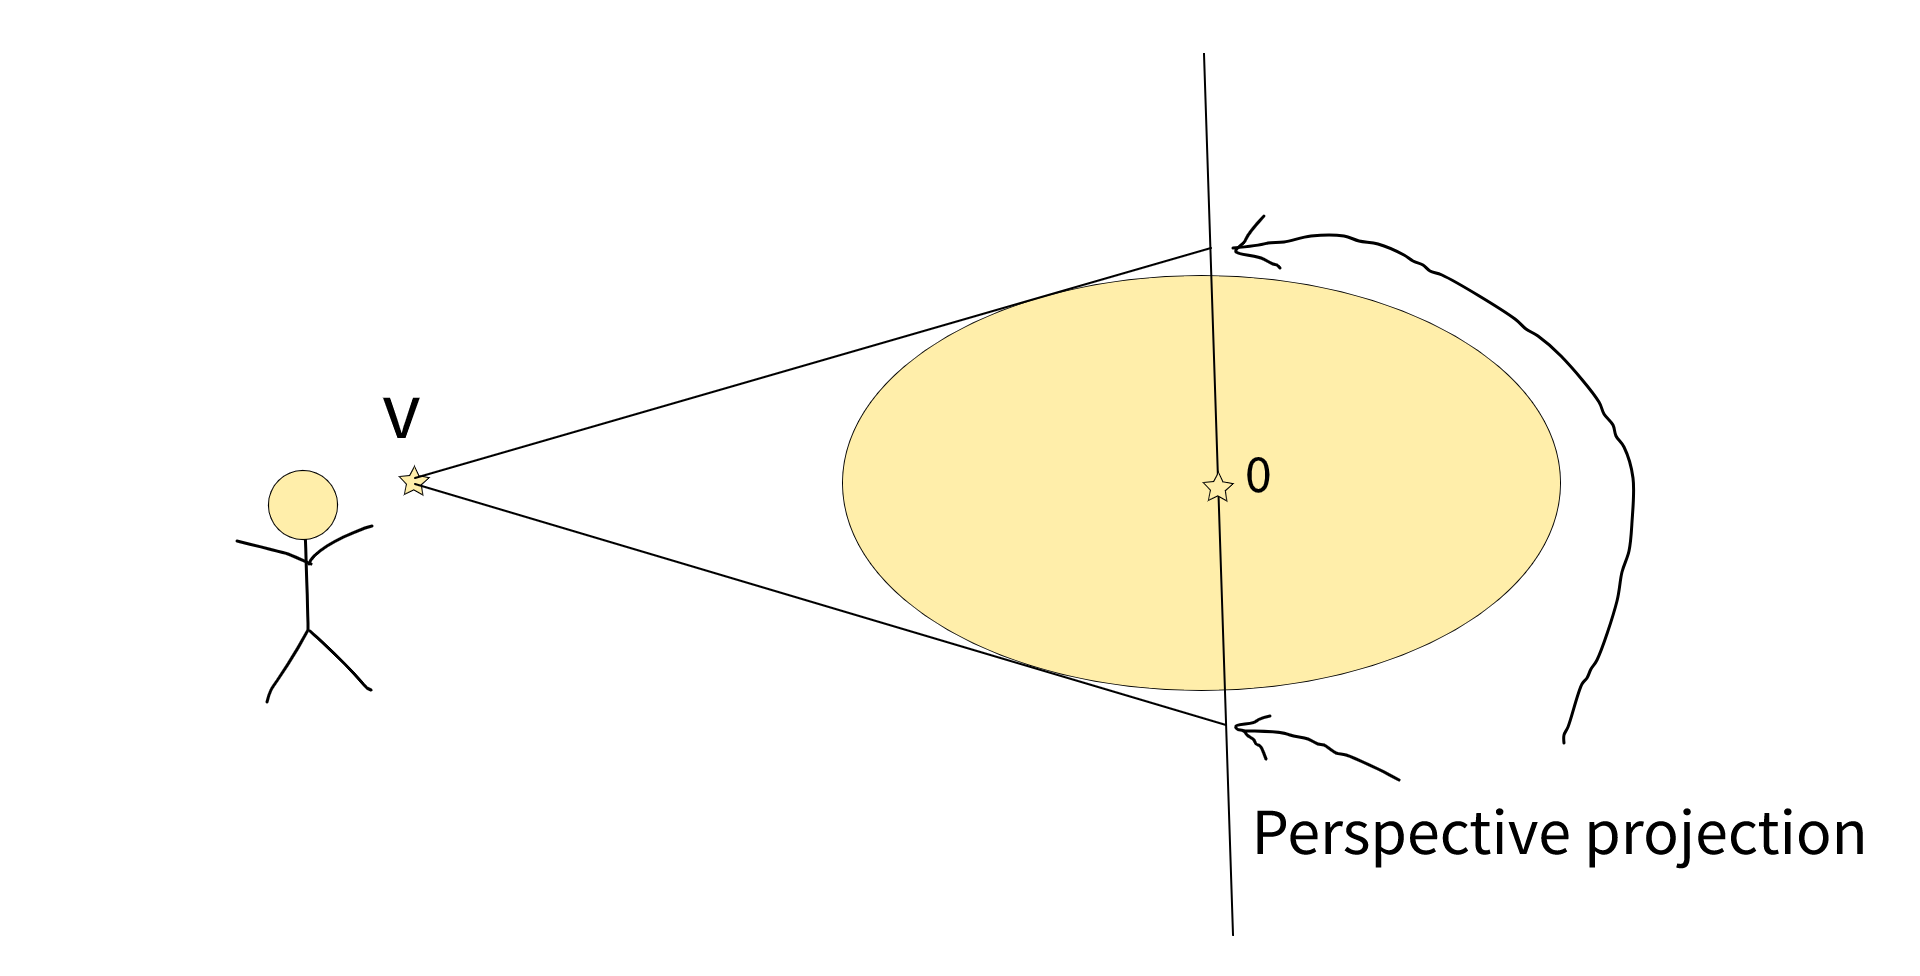
\includegraphics[width=300px]{images/perspective_projection.png}
    \caption{
    	A depiction of the perspective projection.
	}
    \label{perspective_projection_depiction}
\end{figure}

First, we compute the projection of the cone, which is simply its intersection with the hyperplane:
\begin{align*}
H_i \cap A_i 
= \left\{x \in \Rn \bigg| \left(v^{(i)}\right)^Tx = 0, -\frac{\left(x - v^{(i)}\right)^T}{\|x - v^{(i)}\|}\frac{v^{(i)}}{\|v^{(i)}\|}\ge \beta \right\} \\
= \left\{x \in \Rn \bigg| \left(v^{(i)}\right)^Tx = 0, \|v^{(i)}\|\ge \beta\|x - v^{(i)}\| \right\} \\
= \left\{x \in \Rn \bigg| \left(v^{(i)}\right)^Tx = 0, \|x - v^{(i)}\|^2 \le \frac 1 {\beta^2}\|v^{(i)}\|^2 \right\} \\
= \left\{x \in \Rn \bigg| \left(v^{(i)}\right)^Tx = 0, \|x\|^2 \le \left(\frac 1 {\beta^2} - 1\right)\|v^{(i)}\|^2 \right\} \\
\end{align*}

Then, we can compute the perspective projection of the ellipsoid, similar to \cite{eberly_2013}.
Consider the point $x = v^{(i)} + td$ for some direction $d$ and distance $t$.
If $x$ is on the boundary of the ellipsoid, then:
\begin{align*}
(v^{(i)} + t d - \ck )^T \qk  (v^{(i)} + t d - \ck ) = 1 \\
\Longleftrightarrow (v^{(i)} + t d - \ck )^T \qk  v^{(i)} + t (v^{(i)} + t d - \ck )^T \qk  d - (v^{(i)} + t d - \ck )^T \qk  \ck  = 1 \\
\Longleftrightarrow \left(v^{(i)}\right)^T \qk  v^{(i)} + t d^T \qk  v^{(i)} - \ck ^T \qk  v^{(i)} + t \left(v^{(i)}\right)^T \qk  d + t^2 d^T \qk  d - t \ck ^T \qk  d \\- \left(v^{(i)}\right)^T \qk  \ck  - t d^T \qk  \ck + \ck ^T \qk  \ck  = 1 \\
\Longleftrightarrow \left(d^T\qk d
\right) t^2 + \left(
d^T \qk  v^{(i)} +  \left(v^{(i)}\right)^T \qk  d - \ck ^T \qk  d - d^T \qk  \ck 
\right) t \\ +  \left(
\left(v^{(i)}\right)^T \qk  v^{(i)} - \ck ^T \qk  v^{(i)} - \left(v^{(i)}\right)^T \qk  \ck   + \ck ^T \qk  \ck  - 1
\right) = 0 \\
\Longleftrightarrow \left(d^T\qk d
\right) t^2 + 2\left(
\left(v^{(i)}\right)^T \qk  d - \ck ^T\qk d
\right) t + \\ \left(
\left(v^{(i)}\right)^T \qk  v^{(i)} + \ck ^T \qk  \ck  - 2 \ck ^T \qk  v^{(i)} - 1
\right) = 0
\end{align*}

There are either $0$, $1$, or $2$ values of $t$ for which this equation will have solutions.
The directions from $v^{(i)}$ when it intersects the ellipsoid exactly $1$ time are those whose projection will be on the boundary of the perspective projection of the ellipsoid.
The discriminant for these is $0$.
If we let
\begin{align*}
M_i = 
\qk (v^{(i)} - \ck )\left[\qk (v^{(i)} - \ck )\right]^T \\
- \qk  \left(\left(v^{(i)}\right)^T \qk  v^{(i)} + \ck ^T \qk  \ck  - 2 \ck ^T \qk  v^{(i)} - 1\right),
\end{align*}
we find that that these directions satisfy
\begin{align*}
4\left(\left(v^{(i)}\right)^T \qk  d - \ck ^T\qk d\right)^2 \\
- 4 \left(d^T\qk d\right) \left(\left(v^{(i)}\right)^T \qk  v^{(i)} + \ck ^T \qk  \ck  - 2 \ck ^T \qk  v^{(i)} - 1\right) = 0 \\
\Longleftrightarrow d^TM_id = 0.
\end{align*}

% This used to be a line, but it didn't fit...
% d^T\left[
% \left(\qk (v^{(i)} - \ck )\right)\left(\qk (v^{(i)} - \ck )\right)^T
% - \qk  \left(\left(v^{(i)}\right)^T \qk  v^{(i)} + \ck ^T \qk  \ck  - 2 \ck ^T \qk  v^{(i)} - 1\right)\right]d = 0 \\

Next, let
\begin{align*}
t = -\frac {\left(v^{(i)}\right)^T v^{(i)}}{\left(v^{(i)}\right)^T d } \Longrightarrow
0 = \left(v^{(i)}\right)^T v^{(i)} + t {v^{(i)}}^T d \Longrightarrow
0 = \left(v^{(i)}\right)^T \left(v^{(i)} + t d\right)
\end{align*}
so that $x \in H_i$.
We already know that
\begin{align*}
x = v^{(i)} + t d \Longrightarrow
d = \frac 1 t \left(x - v^{(i)}\right)
\Longrightarrow d^TM_id = \frac 1 {t^2} \left(x - v^{(i)}\right)^TM_i\left(x - v^{(i)}\right) = 0
\end{align*}
so the perspective projection of the boundary of the ellipsoid on the hyper-plane $H_i$ is described by
\begin{align*}
\{x \in \Rn | {v^{(i)}}^Tx = 0, \left(x - v^{(i)}\right)^TM_i\left(x - v^{(i)}\right) = 0\}
\end{align*}

Thus, the ellipsoid is contained in cone $A_i$ if and only if
\begin{align*}
\{x \in \Rn | {v^{(i)}}^Tx = 0, \left(x - v^{(i)}\right)^TM\left(x - v^{(i)}\right) = 0\}
\subseteq \{x \in \Rn | {v^{(i)}}^Tx = 0, \|x - v^{(i)}\|^2 \le \frac 1 {\beta_i^2}\|v^{(i)}\|^2 \} \\
= \{x \in \Rn | {v^{(i)}}^Tx = 0, \|x\|^2 \le \left(\frac 1 {\beta_i^2} - 1\right)\|v^{(i)}\|^2 \}.
\end{align*}

For each $i \in [m]$, define
\begin{align*}
\hat v^{(i)} = \frac{v^{(i)}}{\|v^{(i)}\|} \\
R^i = 2\frac{(\hat v^{(i)} + e_1)(\hat v^{(i)} + e_1)^T}{(\hat v^{(i)} + e_1)^T(\hat v^{(i)} + e_1)} - I
\end{align*}
so that
\begin{align*}
& {R^i}v^{(i)} = \|v^{(i)}\|e_1 & {R^i}^T{R^i} = I & \quad \det({R^i}) \in \{-1, 1\}
\end{align*}
and let $W_i$, $y$, $w_{1,1}$, $w_1$ be defined so that
\begin{align*}
& M_i = {R^i}^T M_i' {R^i} = {R^i}^T\left( \begin{array}{cc}
{w_{1,1}^i} & {w_1^i} \\
{w_1^i}^T	& {W_i}  \\
\end{array} \right){R^i} &
{R^i}x = \left(\begin{array}{c}
0 \\
y
\end{array}\right)
\end{align*}
for all $x$ with $x^Tv = 0$.
Then
\begin{align*}
\left(x - {v^{(i)}}\right)^TM_i\left(x - {v^{(i)}}\right) = 0 \\
\Longleftrightarrow x^TM_ix - 2x^TM_i{v^{(i)}} + {v^{(i)}}^TM_i{v^{(i)}} = 0 \\
\Longleftrightarrow x^T{R^i}^TM_i'{R^i}x - 2x^T{R^i}^TM_i'{R^i}{v^{(i)}} + {v^{(i)}}^T{R^i}^TM_i'{R^i}{v^{(i)}} = 0 \\
\Longleftrightarrow y^T{W_i}y - 2y^T{w_1^i}\|v^{(i)}\| + {w_{1,1}^i}\|v^{(i)}\|^2 = 0 \\
\Longleftrightarrow y^T{W_i}y - 2\|v^{(i)}\|y^T{W_i}{W_i}^{-1}{w_1^i} + \|v^{(i)}\|^2{{w_1^i}}^T{W_i}^{-1}{W_i}{W_i}^{-1}{w_1^i} \\
= - \|v^{(i)}\|^2{w_{1,1}^i} + \|v^{(i)}\|^2{{w_1^i}}^T{W_i}^{-1}{W_i}{W_i}^{-1}{w_1^i} \\
\Longleftrightarrow \left(y - \|v^{(i)}\|{W_i}^{-1}{w_1^i}\right)^T{W_i}\left(y - \|v^{(i)}\|{W_i}^{-1}{w_1^i}\right) = - \|v^{(i)}\|^2{w_{1,1}^i} + \|v^{(i)}\|^2{{{w_1^i}}}^T{W_i}^{-1}{{w_1^i}} \\
\end{align*}

Thus, to find the maximum norm $x$ with $\left(v^{(i)}\right)^Tx = 0$, we wish to compute:
\begin{align*}
\max_{y} & \quad \|y\|^2  \\
 & \left(y - \|v^{(i)}\|{W_i}^{-1}{w_1^i}\right)^T{W_i}\left(y - \|v^{(i)}\|{W_i}^{-1}{w_1^i}\right) = - \|v^{(i)}\|^2{w_{1,1}^i} + \|v^{(i)}\|^2{{w_1^i}}^T{W_i}^{-1}{w_1^i}
\end{align*}

After a change of variables
\begin{align*}
w_c \gets \|v^{(i)}\|{W_i}^{-1}w_1^i \\
w_r \gets  - \|v^{(i)}\|^2{w_{1,1}^i} + \|v^{(i)}\|^2{{w_1^i}}^Tw_c \\
s \gets y - w_c
\end{align*}
this becomes:

\begin{align}
\label{cone_feasibility_check}
\begin{array}{ccc}
\max_{y} & \quad \|s - \left(-w_c\right)\|^2  \\
 & s^T\left(\frac {W_i}{w_r}\right)s = 1
 \end{array}
\end{align}

This is the well known optimization problem of projecting a point onto the surface of an ellipsoid.
No explicit solution exists, which leaves us to believe that there is no explicit formulation of finding the maximum volume ellipsoid contained within the intersection of these cones.
However, there is an efficient, binary-search algorithm to solve this \cite{projecttoellipsoid}.


Namely, given 
$p \in \Rn$ and a positive definite, symmetric, $n \times n$ matrix $Q$,
we can consider how to project the point $p$ onto the ellipsoid $\left\{x \in \Rn \bigg | x^TQx = 1 \right\}$:
\begin{align*}
\begin{array}{ccc}
x^{\star} = &\argmin_{x \in \Rn} & \|x - p\|^2 \\
& \textrm{s.t.} & x^TQx = 1.
\end{array}
\end{align*}
If $p^TQp \le 1$, then clearly $x^{\star} = p$.
Otherwise, the first order optimality conditions imply the existence of a $\lambda \in \reals$ such that
% x^{\star} - p = \lambda Qx^{\star} \Longleftrightarrow \left(Q - \frac 1 {\lambda} I\right)x^{\star} = -\frac 1 {\lambda}p \\
\begin{align*}
x^{\star} - p = \lambda Qx^{\star} %\Longleftrightarrow \left(\lambda Q - I\right)x^{\star} = -p
\Longleftrightarrow x^{\star} = -\left(\lambda Q - I\right)^{-1}p
\end{align*}
provided the inverse exists.
Using $\left(x^{\star}\right)^TQx^{\star} = 1$, the problem reduces to finding zeros of the function $f : \reals_+ \to \reals$ defined by
\begin{align*}
f(\lambda) = p^T\left(\lambda Q - I\right)^{-1}Q\left(\lambda Q - I\right)^{-1}p - 1.
\end{align*}
Notice that $f(0) = p^TQp - 1 > 0$, and the presence of $\lambda$ within inverse expressions suggests $\lim_{\lambda \to \infty}f(\lambda) = -1$.
The authors show that a binary search on $\lambda$ can find the zeros of $f$.

% \subsubsection{Numerical Solution}
% 
% Although the algorithm presented in \cref{ideal_ellipsoid_in_polyhedron} yields a solution that cannot be solved explicitly, it is easy to check if an ellipsoid is feasible using \cref{cone_feasibility_check}.
% One very simple random-search algorithm can be used to show this.
% 
% \begin{comment}
% Dramatically simplify this algorithm...
% \end{comment}
% 
% \begin{algorithm}[H]
%     \caption{Search for feasible ellipsoid}
%     \label{numerical_ellipsoid_algorithm}
%     \begin{itemize}
%         \item[\textbf{Step 0}] \textbf{(Initialization)} \\
%                 Set $E_{max}$ to any feasible ellipsoid, 
%                 an initial sample variance $\sigma^2$, 
%                 a threshold $M$ of iterations per sample variance, 
%                 a decrease ratio $\gamma \in (0, 1)$, 
%                 a variance tolerance $\delta_{\sigma} > 0$
%         
%         \item[\textbf{Step 1}] \textbf{(Random Perturbation)} \\
%             Evaluate the next iterate \begin{itemize}
%                 \item[] Sample a rotation matrix $R$ with variance $\sigma^2$, $\qk \gets R \qk$
%                 \item[] Sample a positive diagonal matrix $D$ with variance $\sigma^2$, $\qk \gets D \qk$
%                 \item[] Sample a translation $c$ bounded by with variance $\sigma^2$, $\ck \gets c + \ck$
%             \end{itemize}
%         
%         \item[\textbf{Step 2}] \textbf{(Check Feasibility)} \\
%             Run feasibility check \cref{cone_feasibility_check} for each constraint.
%             If the new ellipsoid is feasible and larger than $E_{max}$, then 
%             	set $E_{max}$ to this ellipsoid,
%             	set counter $j \gets 0$, and
%             	go to Step 1
%         
%         \item[\textbf{Step 3}] \textbf{(Decrease Sample Variance)} \\
%             If the counter $j \ge M$, then
% 	    	decrease $\sigma^2 \gets \gamma \sigma^2$,
% 	    	set the counter $j\gets 0$, and
% 	    	go to Step 1
%             
%         \item[\textbf{Step 4}] \textbf{(Check for Convergence)} \\
% 	    If $\sigma^2 < \delta_{\sigma}$ \textbf{Return} $E_{max}$.
% 	    Otherwise, 
%         		set counter $j \gets j + 1$, and
%         		go to Step 1
%     \end{itemize}
% \end{algorithm}
% 
% Although not efficient, this can be used to find a large ellipsoid within the buffering cones.


\subsubsection{Spherical Solution}

One simplification that allows an explicit formulation is to restrict the ellipsoid to be a sphere.
Although this will not produce as large an ellipsoid, it may be used as a hot start while searching over all ellipsoids.

To compute the maximum volume sphere, we can maximize the minimum distance from the center of the sphere to any cone.
We once again perform a change of variables, this time subtracting of $\xk$ and rotating $v^{(i)}$ onto $e_1$.
This reduces the problem computing the projection of an arbitrary point $(t, y) \in \Rn$ and the second order cone: $\left\{ x \in \mathbb R^n | \quad x^Te_1 = \beta \|x\| \right\}$ for some $\beta \in \reals$.
We find
\begin{align*}
 \\
x^Te_1 = \beta \|x\| 
 \Longleftrightarrow t^2 = \beta^2 \|te_1  + x - t e_1\|^2 \\
 \Longleftrightarrow t^2 = \beta^2 \left(\|te_1\|^2  + \|x - t e_1\|^2\right) \\
 \Longleftrightarrow t^2 = \beta^2 \left(\|te_1\|^2  + \|x - t e_1\|^2\right) \\
 \Longleftrightarrow t^2 = \beta^2 \left(t^2  + \|y\|^2 \right) \\
 \Longleftrightarrow (1 - \beta^2)t^2 = \beta^2 \|y\|^2 \\
 \Longleftrightarrow \sqrt{\frac{1 - \beta^2}{ \beta^2}} t = \|y\|
\end{align*}

This means, that if we let $\beta' = \sqrt{\frac{1 - \beta^2}{\beta^2}}$, we have
\begin{align*}
\left\{ x \in \mathbb R^n | \quad x^Te_1 = \beta \|x\| \right\} = \left \{(s, x)\in \mathbb R^n | \quad\|x\| \le \beta' s \right\}.
\end{align*}

The projection gives the following optimization problem:
\begin{align*}
\min_{x \in \mathbb R^{n-1}, s \in \mathbb R} & \quad \frac 1 2 \|x - y\|^2 + \frac 1 2 (s - t)^2 \\
	\textrm{s.t.}		& \quad \frac 1 2 \|x\|^2 = \frac 1 2 {\beta'}^2 s^2
\end{align*}
which gives us the Lagrangian:
\begin{align*}
l(x, s, \lambda) = \frac 1 2 \|x - y \|^2 + \frac 1 2 \left(s - t\right)^2 - \lambda \frac 1 2 \left(\|x\|^2 - {\beta'}^2 s^2\right).
\end{align*}

After taking the gradient of the Lagrangian, we find that for some $\lambda \in \reals$:
\begin{align*}
x - y - \lambda x = 0, & \quad s - t + \lambda {\beta'}^2 s = 0 \\
x = \frac {y}{1 - \lambda}, & \quad s = \frac {t}{1 + \lambda {\beta'}^2 }.
\end{align*}

We can substitute this into the constraint to solve for $\lambda$:
\begin{align*}
\|x\| = {\beta'} s \\
\left\|\frac {y}{1 - \lambda}\right\| = {\beta'} \frac {t}{1 + \lambda {\beta'}^2 } \\
\left(1 + \lambda {\beta'}^2\right) \left\|y\right\| = {\beta'}  {t} \left|1 - \lambda\right|
\end{align*}

\begin{align*}
\left\|y\right\| + {\beta'}^2\left\|y\right\|\lambda = t {\beta'} - t {\beta'} \lambda          &   \quad
\left\|y\right\| + {\beta'}^2\left\|y\right\|\lambda = t {\beta'} \lambda - t {\beta'}					\\
\left\|y\right\|-t {\beta'} +\left( {\beta'}^2\left\|y\right\| + t {\beta'} \right)\lambda = 0  &		\\
\lambda = \frac{t {\beta'} - \|y\|}{{\beta'}^2\|y\| + t {\beta'}}                               &		
\end{align*}


Substituting $\lambda$ to find $x$ and $s$:
\begin{align*}
x = \frac {y}{1 - \lambda} 																		
= \frac {y}{1 - \frac{t{\beta'} - \|y\|}{{\beta'}^2\|y\| + t{\beta'}}} 									
= \frac {y\left({\beta'}^2\|y\| + t{\beta'}\right)}{{\beta'}^2\|y\| + t{\beta'} - t{\beta'} + \|y\|} 			
= \frac {{\beta'}^2 + \frac{t{\beta'}}{\|y\|}}{1 + {\beta'}^2}y 											
\end{align*}

\begin{align*}
s = \frac {t}{1 + \lambda{\beta'}^2 } 
= \frac {t}{1 +\frac{t{\beta'} - \|y\|}{{\beta'}^2\|y\| + t{\beta'}}{\beta'}^2 } 
= \frac {t\left({\beta'}^2\|y\| + t{\beta'}\right)}{{\beta'}^2\|y\| + t{\beta'} + \left(t{\beta'} - \|y\|\right){\beta'}^2 } 
= \frac {{\beta'}\|y\| + t}{1 + {\beta'}^2 } 
\end{align*}


Thus, the projected point is
\begin{align*}
\left(\frac{{\beta'} \|y\| + t}{1 + {\beta'} ^ 2}, \frac{{\beta'} ^ 2 + t \frac {{\beta'}}{\|y\|}}{1 + {\beta'} ^ 2}y\right)
\end{align*}

with squared distance
\begin{align*}
\left(\frac{{\beta'} \|y\| + t}{1 + {\beta'} ^ 2} - t\right)^2 + \left\|\frac{{\beta'} ^ 2 + t \frac {{\beta'}}{\|y\|}}{1 + {\beta'} ^ 2}y - y\right\|^2
= \left(\frac{{\beta'} \|y\| + t}{1 + {\beta'} ^ 2} - \frac{t + t{\beta'} ^ 2}{1 + {\beta'} ^ 2}\right)^2 + \left(\frac{{\beta'} ^ 2 + t \frac {{\beta'}}{\|y\|}}{1 + {\beta'} ^ 2} - 1\right)^2\left\|y\right\|^2 \\
= \left(\frac{{\beta'} \|y\| - t{\beta'}^2}{1 + {\beta'} ^ 2}\right)^2 + \left(\frac{{\beta'} ^ 2 + t \frac {{\beta'}}{\|y\|} - 1 - {\beta'} ^ 2}{1 + {\beta'} ^ 2}\right)^2\left\|y\right\|^2 
= \left(\frac{{\beta'} \|y\| - t{\beta'}^2}{1 + {\beta'} ^ 2}\right)^2 + \left(\frac{t {\beta'} - \left\|y\right\|}{1 + {\beta'} ^ 2}\right)^2 \\
= \left(1 + {\beta'}^2\right)^{-2}\left[\left({\beta'}^2 \|y\|^2 - 2\beta' \|y\| t {\beta'}^2  + t^2 {\beta'}^4\right) + \left(t^2{\beta'}^2 - 2 t {\beta'} \|y\| + \|y\|^2\right) \right] \\
= \left(1 + {\beta'}^2\right)^{-2}\left[
\left(1 + {\beta'}^2\right)t^2{\beta'}^2 - 2t{\beta'}\left(1 + {\beta'}^2\right) \|y\| + \left(1 + {\beta'}^2\right)\|y\|^2
\right] \\
= \frac{\left(t \beta' - \|y\|\right)^2}{1 + {\beta'}^2}
\end{align*}

We summarize the previous statements here:


\begin{lemma}
Let $t \in \reals$, $y \in \mathbb R^{n-1}$, and $\beta' > 0$.
Then the point
\begin{align*}
z = \left(1 + {\beta'} ^ 2\right)^{-1} \left({\beta'} \|y\| + t, \left({\beta'} ^ 2 + t \frac {{\beta'}}{\|y\|}\right) y\right)
\end{align*}
satisfies
\begin{align*}
z = \argmin_{\left\|x\right\| \le \beta' s} \left\|x - y\right\|^2 + \left\|s - t\right\|^2 \\
\left\|z - (t, y)\right\|^2 = \left(1 + {\beta'}^2\right)^{-1}\left(t \beta' - \left\|y\right\| \right)^2.
\end{align*}
\end{lemma}

After a shift and rotation from the vertex point $\wik$ and going direction $-\wik$:

\begin{align*}
\hat w^{(i,k)} = \frac {\wik} {\|\wik\|} & \quad \forall i \in [m] \\
R^j = 2 \frac{(e_1 + \hat w^{(i,k)})(e_1 + \hat w^{(i,k)})^T}{(e_1 + \hat w^{(i,k)})^T(e_1 + \hat w^{(i,k)})} - I  & \quad \forall j \in [m],
\end{align*}
we have the following optimization problem:
\begin{align*}
\begin{array} {ccc}
\max_{r \ge 0, c, t^i}	& r & \\
					& t^i = R^j\left(\hat w^{(i,k)} - c\right) 									& \quad \forall i \in [m] \\
					& \beta^2 \left(\beta' e_1^T t^i - \left\|t^i - e_1^T t^j\right\|\right)^2 \ge r			& \quad \forall i \in [m] \\
					& \left(\left(c - w^j\right)^T\hat w^{(i,k)}\right)^2 \ge \beta^2 \|c - \wik\|^2		& \quad \forall i \in [m] \\
					& c \in \tr &
\end{array}
\end{align*}

% 
% \begin{comment}
% What did the following few lines do, again?
% \end{comment}
% 
% \begin{align*}
% \beta^2 \left(\beta' e_1^T t^j - \left\|t^j - e_1^T t^j\right\|\right)^2 \ge r \\
% \beta \left(\beta' e_1^T t^j - \left\|t^j - e_1^T t^j\right\|\right) \ge \sqrt{r} \\
% \beta \beta' e_1^T t^j - \beta \left\|t^j - e_1^T t^j\right\| \ge \sqrt{r} \\
% \beta' e_1^T t^j - \frac 1 {\beta} \sqrt{r} \ge \left\|t^j - e_1^T t^j\right\| \\
% \left( \beta' e_1^T t^j - \frac 1 {\beta} \sqrt{r} \right) ^ 2\ge \left\|t^j - e_1^T t^j\right\|^2 \\
% \end{align*}
% 
% 
% 
% 
% \begin{align*}
%  \left(\beta' e_1^T t^j - \left\|t^j - e_1^T t^j\right\|\right)^2 \ge \frac 1 {\beta^2} r \\
%  \left(\beta' e_1^T t^j\right)^2 - 2\beta' e_1^T t^j \left\|t^j - e_1^T t^j\right\| + \left\|t^j - e_1^T t^j\right\|^2 \ge \frac 1 {\beta^2} r \\
%  \left(\beta' e_1^T t^j\right)^2 - \frac 1 {\beta^2} r + \left\|t^j - e_1^T t^j\right\|^2 \ge 2\beta' e_1^T t^j \left\|t^j - e_1^T t^j\right\|\\
%  \left[\left(\beta' e_1^T t^j\right)^2 - \frac 1 {\beta^2} r + \left\|t^j - e_1^T t^j\right\|^2 \right] ^2\ge 4\left(\beta' e_1^T t^j\right)^2 \left\|t^j - e_1^T t^j\right\|^2\\
% \end{align*}
% 

Notice that this optimization problem is not convex.
Although more efficient formulations may exist, this leads us to believe that it may sometimes be difficult to even compute the maximum volume sphere within our buffering cones.

\subsubsection{Conservative Ellipsoid}
Throughout \cref{possible_ellipsoids} we have considered several inner trust regions.
However, we are not able to show that these formulations satisfy the requirements necessary for convergence.
% not been able to show that these satisfied the requirements stated in \cref{ellipsoids_notation_definitions}.
We were able to find an ellipsoid contained within each \cref{define_fik} that may, in general, be smaller than the largest possible ellipsoid.
Because we analyse this in more depth, we dedicate \cref{constructing_and_analysizing_conservative_ellipsoid} to this.

\subsection{Conservative Ellipsoid Derivation}
\label{constructing_and_analysizing_conservative_ellipsoid}

We state the ellipsoid requirements required for convergence in \cref{ellipsoids_notation_definitions}, and then show the conservative ellipsoid satisfies them.
Note the criteria in \cref{ellipsoids_notation_definitions} only summarize one of many possible sets of criteria sufficient for convergence.

\begin{definition}
\label{ellipsoids_notation_definitions}
For each $k \in \naturals$, suppose we are given $n\times n$, symmetric, positive-definite matrices $\qk$, vectors $\ck \in \Rn$, scalars $\sdk > 0$.
We have the following definitions.
\begin{itemize}
\item The sequence $(\qk, \ck, \sdk)$ is \emph{conditioned} if the condition numbers of $\qk$ are bounded for small enough $\dk$.
That is, there exists a $\sigmamax \ge 1$ and $\dacc > 0$ such that if $\dk \le \dacc$, then
\begin{align}
\sigma\left(Q^{(k)}\right) \le \sigmamax. \label{define_suitable_condition_numbers}
\end{align}
\item The tuple $(\qkpo, \ckpo, \sdkpo)$ is \emph{trusted} if an ellipsoid defined by $\qkpo, \ckpo, \sdkpo$ lies within $ \capcones \cap \trkpo $.
That is,
\begin{align}
\unshiftedellipsoidkpo \subseteq \capcones \cap \trkpo  \label{define_suitable_in_tr}
\end{align}
where
\begin{align}
\unshiftedellipsoid = \left\{x \in \Rn | \left(x - \ck \right)^T \qk \left(x - \ck\right) \le \frac 1 2 {\sdk}^2 \right\} \label{define_unshifed_ellipsoid}
\end{align}
\item The tuple $(\qk, \ck, \sdk)$ is \emph{feasible} if an ellipsoid defined by $\qk, \ck, \sdk$ lies within the feasible region:
\begin{align}
\unshiftedellipsoid \subseteq \feasible.
\end{align}
where $\unshiftedellipsoid$ is defined by \cref{define_unshifed_ellipsoid}
\item The tuple $(\qk, \ck, \sdk)$ is \emph{adjacent} if an ellipsoid defined by $\qk, \ck, \sdk$ is near to the current iterate:
\begin{align}
\xk \in \scaledunshiftedellipsoid \label{define_suitable_close_to_iterate}
\end{align}
where
\begin{align}
\scaledunshiftedellipsoid = \left\{x \in \Rn | \left(x - \ck\right)^T \qk \left(x - \ck\right) \le {\sdk}^2 \right\} \label{define_scaledunshiftedellipsoid}
\end{align}
\item The tuple $(\qk, \ck, \sdk)$ is \emph{non-empty} if
\begin{align}
\unshiftedellipsoid \ne \emptyset
\end{align}
where $\unshiftedellipsoid$ is defined by \cref{define_unshifed_ellipsoid}.
\end{itemize}
\end{definition}

\subsubsection{Definition}

% However, we are able to show that this ellipsoid satisfies each of the requirements stated in \cref{ellipsoids_notation_definitions}.
Here we show how to construct the ellipsoid, and that it is 
trusted and adjacent
according to \cref{ellipsoids_notation_definitions}.
Later, in \cref{ellipsoid_is_feasible_section}, we show that it is feasible for small enough $\dk$.
Note that during iteration $k$, we construct the ellipsoid for the next iteration $k+1$.

% Until the $k$-th models are computed, this will initially be an approximation from the previous iteration:
% \begin{align}
% \approxactiveconstraintskpo = \left\{i \in [m] | \zik \in B_{\infty}(\xkpo, \dkpo)\right\}. \label{define_active_approximation}
% \end{align}

First, we define the set of nearly active constraints $\activeconstraintsk$ by \cref{define_activeconstraints}.
If there are no active constraints, $\activeconstraintsk = \emptyset$, then we simply let
\begin{align}
\qkpo = I, \quad \ckpo = \xkpo, \quad \sdkpo = \dkpo. \label{define_trivial_ellipsek}
\end{align}

However, if $\activeconstraintsk \ne \emptyset$, we compute a feasible direction for these nearly active constraints:
\begin{align}
\huk = -\argmin_{\|u\| = 1} \max_{i \in \activeconstraintsk} u^T \frac{\gmcik}{\left\|\gmcik\right\|}. \label{define_u}
\end{align}
We are interested in constructing a cone of directions that make a negative dot product with each nearly active constraint.
We measure the distance between the direction $\huk$ and the nearest direction not in this cone by computing
\begin{align}
\thetamink = \min_{i \in \activeconstraintsk} \left(-\hgik\right)^T \huk \label{define_thetamink}.
\end{align}
Intuitively, larger values of $\thetamink$ imply $\huk$ is farther from the boundary of the cone.
For simplicity, define $\thetamink = 1$ if $\activeconstraintsk = \emptyset$.
% The vector $\huk$ and and value $\thetamink$ can be computed with the following program:
% \begin{align*}
% \begin{array}{ccc}
% \huk \in \argmax_{u\in\Rn, \pi \in\reals} & \pi \\
% & -u^T \frac{\gmcik}{\left\|\gmcik\right\|} \ge \pi & \forall i \in \activeconstraintsk \\
% & \|u \| = 1& 
% \end{array}.
% \end{align*}
We then buffer the directions about $\huk$ by computing
\begin{align}
\bsk = \beta\dk^{p_{\beta}} + \sqrt{\left[1 - \left(\beta\dk^{p_{\beta}}\right)^2\right]\left[1 - \left(\thetamink\right) ^2\right]} \label{define_bsk}
\end{align}
and defining the cone
\begin{align}
\fcki = \left\{x \in \Rn \; \bigg| \; x = \xkpo + ts, t > 0, \|s\| = 1, s^T\huk \ge \bsk \right\}. \label{define_inner_cone}
\end{align}
This cone is feasible with respect to all nearly active constraints.
This cone is depicted in \cref{feasible_direction}.
\begin{figure}[ht]
    \centering
    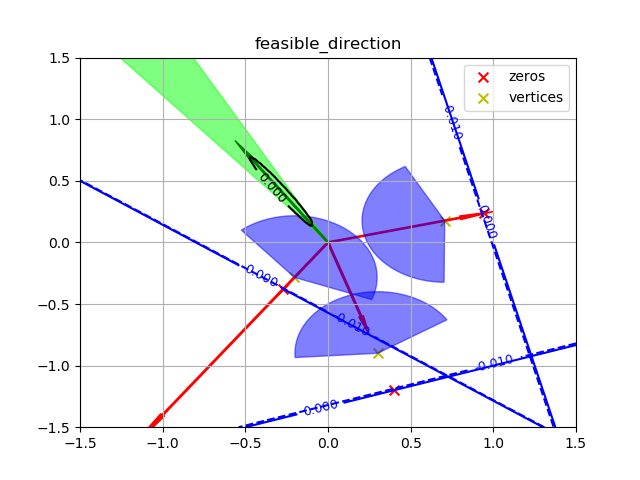
\includegraphics[width=300px]{images/feasible_direction.png}
    \caption{
    	At times, the conservative ellipsoid may be much smaller than desired.
    	Here each cone $\fik$ is in blue, and $\fcki$ is in green.
    	$\fcki$ is contained within the intersection of the $\fik$ cones.
	}
    \label{feasible_direction}
\end{figure}

We then define an ellipsoid within this cone with a helper function
\begin{align}
f_e(\epsilon, \delta, \theta; x) = (x - \epsilon e_1)^T\begin{pmatrix}
1 & \boldsymbol0^T \\
\boldsymbol 0 & \frac{\theta^2}{1 - \theta^2} \boldsymbol I \\
\end{pmatrix}(x - \epsilon e_1) - \frac 1 2 \delta^2 \label{define_ellipse_function}
\end{align}
and rotation matrix
\begin{align}
\rotk = 2\frac{(e_1 + \huk)(e_1 + \huk)^T}{(e_1 + \huk)^T(e_1 + \huk)} - \boldsymbol I \label{define_rotation}
\end{align}
by defining
\begin{align}
\gamma &= 1 + \frac 1 {\sqrt{2}} \label{define_the_constant_gamma} \\
\bs &= \max\left\{\frac 1 2 , \bsk\right\} \label{define_bs} \\
\sampletrkpo &= \left\{x \in \Rn | f_e\left(\frac 1 {2\gamma} \dkpo, \frac 1 {2\gamma} \dkpo,\bs; \rotk(x - \xkpo)\right) \le 0\right\}. \label{define_ellipsek}
\end{align}
Note that within \cref{define_ellipsek} we have defined the components $\qkpo$, $\ckpo$, $\sdkpo$ as
\begin{align}
\qkpo = \left(\rotk\right)^T \begin{pmatrix}
1 & \boldsymbol0^T \\
\boldsymbol 0 & \frac{\bs^2}{1 - \bs^2} \boldsymbol I \\
\end{pmatrix} \rotk, \quad
\ckpo = \xkpo + \frac 1 {2\gamma} \dkpo \huk, \quad
\sdkpo = \frac 1 {2\gamma} \dkpo. \label{conservative_ellipsoid_details}
\end{align}

% \cref{ellsoid_is_suitable_theorem_p2} tells us that this ellipsoid satisfies \cref{ellipsoids_notation_definitions}.
% Which part? Trusted and adjacent

\subsubsection{Properties}
\label{feasible_ellipsoid_analysis}

In this section, we show that our construction of the set $\sampletrk$ as given in 
\cref{define_ellipsek} and \cref{define_trivial_ellipsek}
is trusted and adjacent according to definition \cref{ellipsoids_notation_definitions}.
This is shown within \cref{ellsoid_is_suitable_theorem_p1} and \cref{ellsoid_is_suitable_theorem_p2}.

\begin{lemma}
\label{ellipse_in_cone}
Define $f_e$ by \cref{define_ellipse_function}.
Let $0 < \delta \le \epsilon$ and $\theta > 0$.

We have
\begin{align*}
\left\{x \in \Rn | f_e(\epsilon, \delta, \theta; x) \le 0\right\} \subseteq \left\{tx\in\Rn| e_1^T x \ge \theta,\|x\|=1, t>0\right\}.
\end{align*}
\end{lemma}

\begin{proof}
Let $x$ be such that $f_e(\epsilon, \delta, \theta, x) \le 0$.
First, note that a square is non-negative, so
\begin{align*}
0 \le 2(e_1^Tx - \frac 1 2 \epsilon )^2
= 2(e_1^Tx)^2 - 2e_1^Tx\epsilon + \frac 1 2 \epsilon^2.
\end{align*}
By moving the second and third terms to the right hand side, we find
\begin{align}
(e_1^Tx)^2 \ge \frac 1 2 \epsilon^2 - \left((e_1^Tx)^2 - 2e_1^Tx\epsilon + \epsilon^2\right) 
= \frac 1 2 \epsilon^2 - (e_1^Tx - \epsilon)^2. \label{ellipse_in_cone_eqn1}
\end{align}
If we substitute \cref{define_ellipse_function} into $f_e(\epsilon, \delta, \theta, x) \le 0$, we find that
\begin{align*}
(x - \epsilon e_1)^T\begin{pmatrix}
1 & \boldsymbol0^T \\
\boldsymbol 0 & \frac{\theta^2}{1 - \theta^2} \boldsymbol I \\
\end{pmatrix}(x - \epsilon e_1) \le \frac 1 2 \delta^2
\end{align*}
This can be simplified to
\begin{align*}
(x - \epsilon e_1)^T\begin{pmatrix}
1 & \boldsymbol0^T \\
\boldsymbol 0 & \frac{\theta^2}{1 - \theta^2} \boldsymbol I \\
\end{pmatrix}(x - \epsilon e_1) \\
 = (e_1^Txe_1 + (x - e_1^Txe_1) - \epsilon e_1)^T\begin{pmatrix}
1 & \boldsymbol0^T \\
\boldsymbol 0 & \frac{\theta^2}{1 - \theta^2} \boldsymbol I \\
\end{pmatrix}(e_1^Txe_1 + (x - e_1^Txe_1) - \epsilon e_1)  \\
=
(e_1^Tx - \epsilon)^2 + \frac{\theta^2}{1 - \theta^2}\|x - e_1^Tx e_1\|^2 \le \frac 1 2 \delta^2.
\end{align*}
For a contradiction, suppose that $e_1^Tx < 0$, then $(e_1^Tx - \epsilon)^2 \ge \epsilon^2 \ge \delta^2$.
However, the previous line shows $(e_1^Tx - \epsilon)^2 \le \frac 1 2 \delta^2$.
Thus, $e_1^Tx \ge 0$.
Therefore,
\begin{align*}
(e_1^Tx - \epsilon)^2 + \frac{\theta^2}{1 - \theta^2}\left(\|x\|^2 - (e_1^Tx)^2\right) 
\le (e_1^Tx - \epsilon)^2 + \frac{\theta^2}{1 - \theta^2}\|x - e_1^Tx e_1\|^2 \le \frac 1 2 \delta^2 \le \frac 1 2 \epsilon^2.
\end{align*}
Using \cref{ellipse_in_cone_eqn1}, 
\begin{align*}
\frac{\theta^2}{1 - \theta^2}(\|x\|^2 - (e_1^Tx)^2) \le \frac 1 2 \epsilon^2 - (e_1^Tx - \epsilon)^2 \le (e_1^Tx)^2
\Longrightarrow \|x\|^2 - (e_1^Tx)^2 \le \frac{1 - \theta^2}{\theta^2}(e_1^Tx)^2 \\
\Longrightarrow \|x\|^2 \le \frac 1 {\theta^2}(e_1^Tx)^2
\Longrightarrow e_1^T\frac{x}{\|x\|} \ge \theta
\end{align*}
where we can take the square root because $e_1^Tx \ge 0$.
\end{proof}

\begin{lemma}
\label{ellipse_fits}
Define $f_e$ by \cref{define_ellipse_function}.
We have that $f_e(\delta, \sqrt{2}\delta, \theta; 0) = 0$ for any $\delta, \theta > 0$.
\end{lemma}
\begin{proof}
We compute
\begin{align*}
f_e(\delta, \sqrt{2}\delta, \theta; 0) =(0 - \delta e_1)^T\begin{pmatrix}
1 & \boldsymbol0^T \\
\boldsymbol 0 & \frac{\theta^2}{1 - \theta^2} \boldsymbol I \\
\end{pmatrix}(0 - \delta e_1) - \frac 1 2 (\sqrt 2 \delta)^2
=\delta^2 - \delta^2 = 0.
\end{align*}
% and
% \begin{align*}
% f_e(\delta, \delta, \theta; (1 + \frac{1}{\sqrt{2}}) \delta e_1) =\frac {\delta}{\sqrt{2}}e_1^T\bigg(\begin{pmatrix}
% 1 & \boldsymbol0^T \\
% \boldsymbol 0 & \frac{\theta^2}{1 - \theta^2} \boldsymbol I \\
% \end{pmatrix}\bigg)\frac {\delta}{\sqrt{2}}e_1 - \frac 1 2 \delta^2
% =\frac 1 2 \delta^2 - \frac 1 2 \delta^2 = 0.\\
% \end{align*}
\end{proof}


\begin{lemma}
\label{ellipse_fits_part_2}
Define $f_e$ by \cref{define_ellipse_function}.
Suppose that for some $s \in \Rn$ with $\|s\| = 1$, $s^Te_1 \in \left[\frac 1 2, 1\right]$, $\delta \in [0, \frac 1 2]$ and $f_e(\delta, \delta, \theta; ts) \le 0$.
Then $t \le \left(2 + \sqrt{2}\right) \delta$.
\end{lemma}
\begin{proof}
Notice that $s^Te_1 - \delta \in \left[0, 1\right]$
We let $ts - \delta e_1= \left[\left(ts^Te_1 - \delta\right) e_1 + t\left(s - \left(s^Te_1\right) e_1\right)\right]$
\begin{align*}
f_e(\delta, \delta, \theta; ts) \le 0 \\
\Longrightarrow 
\left[\left(ts^Te_1 - \delta\right) e_1 + t\left(s - \left(s^Te_1\right) e_1\right)\right]^T\begin{pmatrix}
1 & \boldsymbol0^T \\
\boldsymbol 0 & \frac{\theta^2}{1 - \theta^2} \boldsymbol I \\
\end{pmatrix}\left[\left(ts^Te_1 - \delta\right) e_1 + t\left(s - \left(s^Te_1\right) e_1\right)\right] \le \frac 1 2 \delta^2 \\
\Longrightarrow
\left(ts^Te_1 - \delta\right)^2 + t^2\left(s - \left(s^Te_1\right) e_1\right)^2  \frac{\theta^2}{1 - \theta^2} \le \frac 1 2 \delta^2
\Longrightarrow 
\left(t s^Te_1 - \delta\right)^2 \le \frac 1 2 \delta^2 
\Longrightarrow t s^Te_1 - \delta \le \frac 1 {\sqrt{2}} \delta.
\end{align*}
But,
\begin{align*}
\frac 1 2 t \le t s^Te_1 \le \left(1 + \frac 1 {\sqrt{2}}\right) \delta
\Longrightarrow t \le \left(2 + \sqrt{2}\right) \delta.
\end{align*}
\end{proof}




\begin{lemma}
\label{boundbsk}
Let $\bsk$, $\thetamink$, and $p_{\beta}$ be defined by \cref{define_bsk}, \cref{define_thetamink}, and \cref{define_abpab}.

If $\dk^{p_{\beta}} \le \frac {1} {4\beta}\left(\thetamink\right)^2$, then $\bsk \le 1 - \frac 1 4 \left(\thetamink\right)^2$.
\end{lemma}


\begin{proof}


First note that $\thetamink \le 1$ and $p_{\beta} \in (0, 1)$, so that $\beta \dk \le \frac 1 4$.
Because $\left(\thetamink\right)^2 \ge 4\beta\dk^{p_{\beta}}$,
\begin{align*}
    \left[1 - \left(\beta \dk ^{p_{\beta}}\right)^2\right]\left[1 - \left(\thetamink \right)^2\right]
\le \left[1 - \left(\beta \dk ^{p_{\beta}}\right)^2\right]\left[1 - 4\beta \dk^{p_{\beta}}\right] \\
= 1 - 4 \beta \dk^{p_{\beta}} - \left(\beta \dk^{p_{\beta}}\right)^2 + 4 \left(\beta \dk^{p_{\beta}}\right)^3 \\
= \left(1 - 2 \beta \dk^{p_{\beta}}\right)^2 - 5 \left(\beta\dk^{p_{\beta}}\right)^2 + 4 \left(\beta \dk^{p_{\beta}}\right)^3 \\
\le \left(1 - 2\beta\dk^{p_{\beta}}\right)^2.
\end{align*}
Thus, 
\begin{align}
\label{steves_rewrite_eqn1}
\sqrt{\left[1 - \left(\beta \dk ^{p_{\beta}}\right)^2\right]\left[1 - \left(\thetamink \right)^2\right]} 
\le 1 - 2 \beta \dk^{p_{\beta}}.
\end{align}
Note also that $1 - \left(\beta  \dk ^{p_{\beta}}\right)^2 \le 1$, so
\begin{align}
\label{steves_rewrite_eqn2}
\sqrt{\left[1 - \left(\beta \dk ^{p_{\beta}}\right)^2\right]\left[1 - \left(\thetamink \right)^2\right]} 
\le \sqrt{1 - \left(\thetamink \right)^2} \le 1 - \frac 1 2 \left(\thetamink \right)^2.
\end{align}
Adding \cref{steves_rewrite_eqn1} and \cref{steves_rewrite_eqn2}, we find
\begin{align*}
2 \sqrt{\left[1 - \left(\beta \dk ^{p_{\beta}}\right)^2\right]\left[1 - \left(\thetamink \right)^2\right]} 
\le 2 - 2 \beta \dk ^{p_{\beta}} - \frac 1 2 \left(\thetamink \right)^2
\end{align*}
and
\begin{align*}
\bsk = \beta \dk ^{p_{\beta}} + \sqrt{\left[1 - \left(\beta \dk ^{p_{\beta}}\right)^2\right]\left[1 - \left(\thetamink \right)^2\right]}
\le \beta \dk ^{p_{\beta}} + 1 - \beta \dk ^{p_{\beta}} - \frac 1 4 \left(\thetamink \right)^2 \\
= 1 - \frac 1 4 \left(\thetamink \right)^2.
\end{align*}
\end{proof}

% \begin{proof}
% For any $0 < \epsilon < 1$ there exists $\dacco(\epsilon) > 0$, such that for any $k \in \naturals$ with
% $\thetamink \ge \epsilon$ and $\dk \le \dacco(\epsilon)$, we have
% $\bsk \le 1 - \frac 1 4 \epsilon^2$.
% Let $\alpha$, $\beta$, $p_{\alpha}$, and $p_{\beta}$ be defined by \cref{define_abpab}.
% % Also, let $\minangledelta$ be defined as in \cref{minangleassumption}.
% Then we can let $\dacco(\epsilon)$ be defined by
% % \minangledelta,
% % 1,
% \begin{align}
% \dacco(\epsilon) < \min\left\{
% \left(\frac {\epsilon ^2} {4\beta} \right)^{\frac 1 {p_{\beta}}},
% \left(\frac 1 {2\beta}\right)^{\frac 1 {p_{\beta}}}
% \right\}\label{define_delta_accuracy_old}.
% \end{align}
% If $\dk \le \dacco(\epsilon)$, then
% \begin{align}
% \beta\dk^{p_{\beta}} \le \frac 1 {4} \epsilon^2 \quad \textrm{and}\label{boundedbeta_deltasmall_2} \\
% 2\beta\dk^{p_{\beta}} \le 1. \label{boundedbeta_deltasmall_3}
% \end{align}
% Rearranging \cref{boundedbeta_deltasmall_2}, provides $-\epsilon^2 \le -4\beta\dk^{p_{\beta}}$,
% which combined with $\epsilon ^2 \le 1 \le 5$ shows
% \begin{align*}
% -\left[5- \epsilon^2\right]\left(\beta\dk^{p_{\beta}}\right)^2  - \epsilon^2 \le -4\beta\dk^{p_{\beta}}.
% \end{align*}
% This means
% \begin{align*}
% \left(1 - \epsilon^2\right)\left(1 - \left(\beta\dk^{p_{\beta}}\right)^2\right) 
% = 1 - \epsilon^2 - \left[5 - \epsilon^2\right]\left(\beta\dk^{p_{\beta}}\right)^2 + 4\left(\beta\dk^{p_{\beta}}\right)^2 \\
% \le 1 - 4\beta\dk^{p_{\beta}} + 4\left(\beta\dk^{p_{\beta}}\right)^2 = \left(1 - 2\beta\dk^{p_{\beta}}\right)^2.
% \end{align*}
% Dividing by $1 - \left(\beta\dk^{p_{\beta}}\right)^2$, taking the square root, and then dividing by $2$ we see
% % 1 - \epsilon^2 \le \frac{\left(1 - 2\beta\dk^{p_{\beta}}\right)^2}{1 - \left(\beta\dk^{p_{\beta}}\right)^2}
% % \Longrightarrow
% \begin{align}
% \frac 1 2 \sqrt{1 - \epsilon^2} \le \frac 1 2 \frac{1 -2\beta\dk^{p_{\beta}}}{\sqrt{1 - \left(\beta\dk^{p_{\beta}}\right)^2}}
% = \frac{\frac 1 2 -\beta\dk^{p_{\beta}}}{\sqrt{1 - \left(\beta\dk^{p_{\beta}}\right)^2}}. \label{boundedbeta_eqn1}
% \end{align}
% Here, \cref{boundedbeta_deltasmall_3} ensures that the denominator is positive.
% Also,
% \begin{align*}
% 1 - \epsilon^2 \le 1 - \epsilon^2 + \frac 1 4 \epsilon^4 
% = \left(1 - \frac 1 2 \epsilon^2 \right)^2 
% \Longrightarrow 1 \le \frac{\left(1 - \frac 1 2 \epsilon^2\right)^2}{1 - \epsilon^2}
% \end{align*}
% so that
% \begin{align*}
% 1 - \left(\beta\dk^{p_{\beta}}\right)^2 \le 1 \le \frac{\left(1 - \frac 1 2 \epsilon^2\right)^2}{1 - \epsilon^2} 
% \Longrightarrow \sqrt{1 - \left(\beta\dk^{p_{\beta}}\right)^2}\le \frac{1 - \frac 1 2 \epsilon^2}{\sqrt{1 - \epsilon^2} } 
% \Longrightarrow \sqrt{1 - \epsilon^2} \le \frac{1 - \frac 1 2 \epsilon^2}{\sqrt{1 - \left(\beta\dk^{p_{\beta}}\right)^2}}.
% \end{align*}
% Dividing by $2$ yields:
% \begin{align}
% \frac 1 2 \sqrt{1 - \epsilon^2} \le \frac{\frac 1 2 - \frac 1 4 \epsilon^2}{\sqrt{1 - \left(\beta\dk^{p_{\beta}}\right)^2}}
% \label{boundedbeta_eqn2}.
% \end{align}
% 
% We then add \cref{boundedbeta_eqn1} and \cref{boundedbeta_eqn2} to find
% \begin{align*}
% \sqrt{1 - \epsilon^2} \le \frac{1 -  \frac 1 4 \epsilon^2 - \beta\dk^{p_{\beta}}}{\sqrt{1 - \left(\beta\dk^{p_{\beta}}\right)^2}}
% \Longrightarrow \beta\dk^{p_{\beta}} + \left(\sqrt{1 - \epsilon^2}\right)\sqrt{1 - \left(\beta\dk^{p_{\beta}}\right)^2} \le 1 -  \frac 1 4 \epsilon^2.
% \end{align*}
% Because $\thetamink \ge \epsilon$, we have $\sqrt{1 - \epsilon^2} \ge \sqrt{1 - \left(\thetamink\right)^2}$
% so that
% \begin{align*}
% \bsk 
% = \beta\dk^{p_{\beta}} + \sqrt{\left(1 - \left(\beta\dk^{p_{\beta}}\right)^2\right)\left(1 - \left(\thetamink\right)^2\right)} 
% \le \beta\dk^{p_{\beta}} + \left(\sqrt{1 - \epsilon^2}\right)\sqrt{1 - \left(\beta\dk^{p_{\beta}}\right)^2} \\
% \le 1 -  \frac 1 4 \epsilon^2.
% \end{align*}
% \end{proof}



\begin{lemma}
\label{boundbeta}
Let $\thetamink$ and $\qkpo$ be defined by \cref{define_thetamink} and \cref{define_ellipsek} respectively.

If $\dk \le \frac 1 {4 \beta} \left(\thetamink\right)^2$, then $\sigma\left(\qkpo\right) \le 12 \left(\thetamink\right)^{-2}$.

% For any $0 < \epsilon < 1$ there exists $\dacco(\epsilon) > 0$, such that for any $k \in \naturals$ with
% $\thetamink \ge \epsilon$ and $\dk \le \dacco(\epsilon)$, we have $\sigma(\qkpo) \le \frac{12}{\epsilon^2}$.
\end{lemma}

\begin{proof}
Let $\rotk$, and $\gamma$ be defined as in \cref{define_rotation}, and \cref{define_the_constant_gamma} respectively.
Also, during iteration $k$, let $\bs$ be defined by \cref{define_bs}.
% Definition \cref{define_ellipsek} states
% \begin{align*}
% \qk = \rotk^T \begin{pmatrix}
% 1 & \boldsymbol0^T \\
% \boldsymbol 0 & \frac{\bs^2}{1 - \bs^2} \boldsymbol I \\
% \end{pmatrix} \rotk, \quad
% \ck = \xk  + \frac 1 {2\gamma} \dk\huk, \quad
% \sdk = \frac 1 {2\gamma} \dk.
% \end{align*}
First note that by \cref{define_bs} and \cref{boundbsk}, we have
$\frac 1 2 \bsk \le 1 - \frac 1 4 \left(\thetamink\right)^2$.
Squaring this yields
\begin{align}
\frac {1} 4 \le \left(\bs\right)^2 \le \left(1 - \frac 1 4 \left(\thetamink\right)^2\right)^2 \le 1 - \frac 1 4 \left(\thetamink\right)^2 \label{p2_numerator}
\end{align}
so that
\begin{align}
\frac 1 4  \left(\thetamink\right)^2 \le 1 - \left(\bs\right)^2 \le \frac 3 4. \label{p2_denominator}
\end{align}
Dividing \cref{p2_numerator} by \cref{p2_denominator}, we see that
\begin{align*}
\frac 1 3
\le \frac{\left(\bs\right)^2}{1 - \left(\bs\right)^2}
\le \frac {4 - \left(\thetamink\right)^2}{\left(\thetamink\right)^2} \le \frac {4}{\left(\thetamink\right)^2}
\end{align*}
Now, using \cref{conservative_ellipsoid_details}, we can compute 
\begin{align*}
\sigma \left(\qkpo\right) 
= \frac{\max\left\{1, \frac{\left(\bs\right)^2}{1 - \left(\bs\right)^2}\right\}}{\min\left\{1, \frac{\left(\bs\right)^2}{1 - \left(\bs\right)^2}\right\}} 
\le \frac {12}{\left(\thetamink\right)^2}
\end{align*}
as $\det(\rotk) = 1$.
\end{proof}




\begin{lemma}
\label{cone_subset_cone}
Given $u, v \in \Rn$, and $\gamma, \beta \in (0, 1]$ that satisfy $\|u\| = \|v\|= 1$, $u^Tv = \gamma > \beta > 0$, define
\begin{align*}
B = \{x\in\Rn | {v}^Tx \ge \beta\|x\|\}, \quad
S = \left\{x\in\Rn \bigg| v^Tx \ge \left(\beta\gamma + \sqrt{(1 - \beta^2)\left(1 - \gamma^2\right)}\right)\|x\| \right\}. 
\end{align*}
Then, $S \subseteq B$.
\end{lemma}

\begin{proof}
For a contradiction, let $y \in \Rn$ be such that $y \not \in B$ and $y \in S$ and define $\hat y = \frac{y}{\|y\|}$.
That is,
\begin{align}
v^T\hat y < \beta \label{csc_vy} \\
u^T\hat y \ge \beta\gamma + \sqrt{\left(1 - \beta^2\right)\left(1 - \gamma^2\right)}. \label{csc_uy}
\end{align}

Define
\begin{align*}
x^{\star} = \beta v + \sqrt{\frac{1 - \beta^2}{1 - \gamma^2}} (u - \gamma v )
\end{align*} and notice that
\begin{align}
\begin{array}{ccccc}
{u}^Tx^{\star} &=& \beta\gamma + \sqrt{\frac{1 - \beta^2}{1 - \gamma^2}} (1 - \gamma^2) &=&  \beta\gamma + \sqrt{\left(1 - \beta^2\right)\left(1 - \gamma^2\right)} \\
{v}^Tx^{\star} &=& \beta + \sqrt{\frac{1 - \beta^2}{1 - \gamma^2}}(\gamma - \gamma) &=& \beta \\
{x^{\star}}^Tx^{\star} &=& \beta^2 + 2\beta\sqrt{\frac{1 - \beta^2}{1 - \gamma^2}}(\gamma - \gamma) + \frac{1 - \beta^2}{1 - \gamma^2} (1- 2\gamma^2 + \gamma^2)&=& 1.
\end{array}. \label{csc_vx_ux}
\end{align}

Using \cref{csc_vx_ux} and \cref{csc_uy}, we see that
\begin{align*}
\beta\gamma + \sqrt{\left(1 - \beta^2\right)\left(1 - \gamma^2\right)} \le {u}^T\hat y = {u}^T\left(x^{\star} + \hat y - x^{\star}\right) 
= \beta \gamma + \sqrt{(1 - \beta^2)\left(1 - \gamma^2\right)} + {u}^T\left(\hat y - x^{\star}\right).
\end{align*}
Subtracting $\beta\gamma + \sqrt{\left(1 - \beta^2\right)\left(1 - \gamma^2\right)}$ from both sides, we find that
\begin{align}
{u}^T\left(\hat y - x^{\star}\right) \ge 0 \label{csc_uymx}.
\end{align}
Likewise, we can use \cref{csc_vx_ux} and \cref{csc_vy} to provide
\begin{align*}
\beta > {v}^T\hat y = {v}^T\left(x^{\star} + \hat y - x^{\star}\right) = \beta + {v}^T\left(\hat y - x^{\star}\right).
\end{align*}
After subtracting $\beta$ from both sides, we see
\begin{align}
{v}^T\left(\hat y - x^{\star}\right) < 0 \Longrightarrow -{v}^T\left(\hat y - x^{\star}\right) > 0. \label{csc_vymx}
\end{align}
% which means $\hat y \ne x^{\star}$.
Lastly, we will need
\begin{align}
\gamma > \beta 
\Longrightarrow 1 - \beta^2 > 1 - \gamma^2
\Longrightarrow \sqrt{\frac{1 - \beta^2}{1 - \gamma^2}} > 1
\Longrightarrow \gamma \sqrt{\frac{1 - \beta^2}{1 - \gamma^2}} - \beta > 0. \label{csc_gamma_beta_positive}
\end{align}
Now, we can compute
\begin{align*}
{\left(\hat y - x^{\star}\right)}^Tx^{\star} = 
\beta {\left(\hat y - x^{\star}\right)}^Tv
+ \sqrt{\frac{1 - \beta^2}{1 - \gamma^2}} 
\left(u^T\left(\hat y - x^{\star}\right) - \gamma v^T \left(\hat y - x^{\star}\right) \right)\\ 
= \left[\gamma \sqrt{\frac{1 - \beta^2}{1 - \gamma^2}} - \beta\right] \left[-v^T\left(\hat y - x^{\star}\right)\right]
+ \left[\sqrt{\frac{1 - \beta^2}{1 - \gamma^2}}\right] \left[u^T\left(\hat y - x^{\star}\right) \right] > 0.
\end{align*}
because \cref{csc_uymx}, \cref{csc_vymx}, and \cref{csc_gamma_beta_positive} show that the first product is postive and the second product is non-negative.
However, this is a contradiction as
\begin{align*}
1 = \|\hat y\|^2 = \|x^{\star} + \hat y - x^{\star}\|^2 = \|x^{\star}\|^2 + 2{\left(\hat y - x^{\star}\right)}^Tx^{\star} + \|\hat y - x^{\star}\|^2 > \|x^{\star}\|^2 = 1
\end{align*}
and there is no such $y$.
Thus, any $y \in\Rn$ with $y \in S$ must also have $y \in B$.
\end{proof}


\begin{lemma}
\label{large_zik_means_means_no_intersection}
Let
$\zik$ and $\fik$
be defined by
\cref{define_z} and \cref{define_fik} respectively.
For any $R > 0$ and $K > R\sqrt{n}$, there exists $\deltalargzik > 0$ such that if $\dk \le \deltalargzik$ and 
\begin{align*}
\zik \not \in B_{\infty}\left(\xk, (1+K) \dk\right),
\end{align*}
then $B_{\infty}\left(\xk, R \dk\right) \subseteq \fik$.
\end{lemma}
\begin{proof}
Let $\alpha$, $\beta$, $p_{\alpha}$, and $p_{\beta}$ be defined by \cref{define_abpab}.
We can define
\begin{align}
\deltalargzik = \min\left\{
\left(\frac 1 {\beta }\frac {K - R\sqrt{n}}{K + R\sqrt{n}}\right)^{\frac 1 {p_{\beta }}},
\left(\frac 1 {(1+K)\alpha}\right)^{\frac 1 {p_{\alpha}}}
\right\} \label{define_deltalargzik}
\end{align}
and suppose that $\|\xk - \zik\| \ge (1+K) \dk$.

First, note that by \cref{define_w}
\begin{align*}
\|\xk - \wik\| = (1 - \alpha\dk^{p_{\alpha}}) \|\xk - \zik\| \ge \frac {K} {(1+K)} (1+K)\dk = K\dk.
\end{align*}

Let $y \in B_{\infty}\left(\xk, R \dk\right)$, so that $\|y - \xk\| \le \sqrt{n}R\dk$.
Also, define
\begin{align*}
t  = \frac{(y - \wik)^T(\xk - \wik)}{\left(\xk - \wik\right)^T(\xk - \wik)} \\
p = \wik + t\left(\xk - \wik\right)
\end{align*}
so that
\begin{align*}
\|y - \wik\| \le \|y - \xk\| + \|\xk - \wik\| \\
\Longrightarrow \frac{\|y - \wik\|}{\|\xk - \wik\|} \le 1 +  \frac{\|y - \xk\|}{\|\xk - \wik\|} 
\le 1 + \frac{\sqrt{n}R\dk}{K \dk} = \frac {K+R\sqrt{n}}{K} \\
\Longrightarrow \frac{\|\xk - \wik\|}{\|y - \wik\|} \ge \frac {K}{K+R\sqrt{n}}
\end{align*}
and
\begin{align*}
\left(y - p\right)^T\left(\xk - \wik\right) = 
\left(y - \wik - t\left(\xk - \wik\right)\right)^T\left(\xk - \wik\right) \\
= \left(y - \wik\right)^T\left(\xk - \wik\right) - t\left(\xk - \wik\right)^T\left(\xk - \wik\right) = 0.
\end{align*}
Because
\begin{align*}
\|\xk - p\| = \|\xk - \wik + \wik - p\| = \left\|\xk - \wik - t\left(\xk - \wik\right)\right\| \\
= (1-t)\|\xk - \wik\| \ge (1-t)K\dk
\end{align*}
we have
\begin{align*}
nR^2\dk^2 \ge \|\xk - y\|^2 = \|\xk - p\|^2 + \|y - p\|^2 \ge K^2(1-t)^2\dk^2 
\Longrightarrow 1-t \le \frac {R\sqrt{n}} {K} 
\Longrightarrow t \ge \frac {K - R\sqrt{n}}{K}
\end{align*}

Putting this together, we see
\begin{align*}
\frac{\xk - \wik}{\left\|\xk - \wik\right\|}^T\frac{y - \wik}{\left\|y - \wik\right\|} 
= \frac{\left(\xk - \wik\right) ^T\left(y - p\right) + \left(\xk - \wik\right)^T\left(p - \wik\right)}{\left\|\xk - \wik\right\|\left\|y - \wik\right\|} \\
= t\frac{\left(\xk - \wik\right)^T\left(\xk - \wik\right)}{\left\|\xk - \wik\right\|\left\|y - \wik\right\|}
= t \frac{\left\|\xk - \wik\right\|}{\left\|y - \wik\right\|}
= \frac {K - R\sqrt{n}}{K + R\sqrt{n}} \ge \beta \dk^{p_{\beta}}.
\end{align*}
% \ge \frac {K - \sqrt{n}}{K} \frac {K}{K+\sqrt{n}}
\end{proof}

\begin{lemma}
\label{inner_cone_inside_each_cone}
Let $\fcki$ and $\capcones$ be defined by \cref{define_inner_cone} and \cref{define_capcones} respectively.
If 
% $\dk \le 1$ and 
$\xkpo \in \capcones$, then $\fcki \subseteq \capcones$.
\end{lemma}
% \left(\frac 1 {\beta} \sqrt{\frac 3 4}\right)^{\frac 1 {p_{\beta}}}

\begin{proof}
Let 
$\huk$, $\bsk$, $\thetamink$, $\activeconstraintsk$, and $\fik$
be defined by
\cref{define_u}, \cref{define_bsk}, \cref{define_thetamink}, \cref{define_activeconstraints}, and \cref{define_fik} 
respectively and $\alpha$, $\beta$, $p_{\alpha}$, $p_{\beta}$ be defined by \cref{define_abpab}.
Fix some $i \in \activeconstraintsk$, and define $\gamma_i = -\left(\huk\right)^T\hgik$ as well as
\begin{align*}
S_1 = \left\{s\in\Rn | \quad s^T\huk\ge\bsk\|s\| \right\} \\
S_2 = \left\{s\in\Rn | \quad s^T\huk\ge\left[\beta\dk^{p_{\beta}}\gamma_i + \sqrt{(1 - \left(\dk^{p_{\beta}}\beta\right)^2)\left(1 - \gamma_i^2\right)}\right]\|s\| \right\} \\
S_3 = \left\{s\in\Rn | \quad s^T\left(-\hgik\right)\ge\beta\dk^{p_{\beta}}\|s\| \right\}
\end{align*}
The set $S_1$ is that set of all feasible directions from $\xk$ for $\fcki$, and $S_3$ is that set of all feasible direction from $\wik$ for $\fik$.
Because $\xkpo \in \fik$, $\fcki \subseteq \fik$ follows from $S_1 \subseteq S_3$.
We show this next.


% = -\frac{m_{c_i}(\xk)}{\|\gmcik\|}\frac{\|\gmcik\|}{m_{c_i}(\xk)}
% Now, we show that $S_1 \subseteq S_3$.
By letting $u \gets \huk$, $v \gets -\hgik$, $\beta \gets \beta \dk^{p_{\beta}}$, \cref{cone_subset_cone} tells us that
$S_2 \subseteq S_3$.
But $\gamma_i \ge \thetamink$, so that
\begin{align*}
\beta\dk^{p_{\beta}}\gamma_i + \sqrt{\left(1 - \left(\beta\dk^{p_{\beta}}\right)^2\right)\left(1 - \gamma_i^2\right)}
\le \max_{i\in\activeconstraintsk} \left(\beta\dk^{p_{\beta}}\gamma_i + \sqrt{\left(1 - \left(\beta\dk^{p_{\beta}}\right)^2\right)\left(1 - \gamma_i^2\right)}\right) \\
\le \beta\dk^{p_{\beta}} \max_{i\in\activeconstraintsk}\left\{\gamma_i\right\} + \sqrt{\left(1 - \left(\beta\dk^{p_{\beta}}\right)^2\right)\left(1 - \left(\min_{i\in\activeconstraintsk}\left\{\gamma_i\right\}\right)^2\right)} \\
\le \beta\dk^{p_{\beta}} + \sqrt{\left(1 - \left(\beta\dk^{p_{\beta}}\right)^2\right)\left(1 - \left(\thetamink\right)^2\right)} = \bsk
\end{align*}

and for any $s\in S_1$,
\begin{align*}
\left(\frac{s}{\|s\|}\right)^T\huk \ge \bs 
\ge \beta\dk^{p_{\beta}}\gamma_i + \sqrt{(1 - \dk^{2p_{\beta}}\beta^2)\left(1 - \gamma_i^2\right)}
\Longrightarrow s \in S_2 \subseteq S_3.
\end{align*}

Thus, $\fcki \subseteq \fik$.
\end{proof}


% \color{red}
% The red is no longer needed.
% First, we show that $\xk \in \fik$.
% We see that:
% \begin{align*}
% \xk = \xk + \left(1 - \alpha\dk^{p_{\alpha} }\right)(\zik - \xk) - \left(1 - \alpha\dk^{p_{\alpha} }\right)(\zik - \xk)
% \end{align*}
% where
% \begin{align*}
% \frac{-\left(1 - \alpha\dk^{p_{\alpha} }\right)(\zik - \xk)}{\left\|-\left(1 - \alpha\dk^{p_{\alpha} }\right)(\zik - \xk)\right\|}^T\hgik = 1 \ge \beta \dk^{p_{\beta}}
% \end{align*}
% because $\dk \le 1$.
% \color{black}


\begin{lemma}
\label{ellsoid_is_suitable_theorem_p1}
Let $\activeconstraintsk$ and $\omegainc$ be defined by \cref{define_activeconstraints} and \cref{define_the_omegas} respectively.
If $\activeconstraintsk = \emptyset$ and $\dkpo \le \omegainc\dk$, 
then there exists $\deltalargzik>0$ such that if $\dk \le \deltalargzik$ the
ellipsoids defined by \cref{define_trivial_ellipsek} 
are trusted, and adjacent according to \cref{ellipsoids_notation_definitions}.

% satisfy \cref{ellipsoids_notation_definitions}.
\end{lemma}
\begin{proof}
Also, \cref{define_suitable_close_to_iterate} is satisfied because $(\xkpo - \xkpo)^T\qkpo(\xkpo - \xkpo) = 0 \le \sdkpo^2$.
Let $\omegainc$, $\capcones$, $\fik$, and $\zikthresh$ be defined by \cref{define_the_omegas}, \cref{define_capcones}, \cref{define_fik}, and \cref{define_zikthresh} respectively.
Because $\activeconstraintsk = \emptyset$, we can use 
\cref{large_zik_means_means_no_intersection} with $R = (2 + \omegainc)\sqrt{n}$, $K = \zikthresh$ to conclude the existence of $\deltalargzik > 0$ such that 
if $\dk \le \deltalargzik$, then for each 
$i \in [m]$, $\trkpo \subseteq \fik$.
Thus, \cref{define_suitable_in_tr} is satisfied because 
\begin{align*}
\unshiftedellipsoidkpo = \left\{x \in \Rn \bigg| \|x - \xkpo\|^2 \le \dkpo^2 \right\} \subseteq \trkpo \subseteq \capcones.
\end{align*}
\end{proof}


\begin{lemma}
\label{ellsoid_is_suitable_theorem_p2}
Let $\activeconstraintsk$ 
% and $\omegainc$ 
be defined by 
\cref{define_activeconstraints}
% and \cref{define_the_omegas} respectively
.
If $\activeconstraintsk \ne \emptyset$ and $\dk \le 1$, 
then the ellipsoids defined by \cref{define_ellipsek} are trusted and adjacent according to \cref{ellipsoids_notation_definitions}.

% There exsists $\dacc > 0$ such that if $\dk \le \dacc$
% and $\activeconstraintsk \ne \emptyset$
% \begin{align}
% \bs = \max\left\{\frac 1 2, \bsk\right\} \label{define_bs} \\
% \gamma = 1 + \frac 1 {\sqrt 2}
% \end{align}
% where $\dacc$ is defined in \cref{define_delta_accuracy}, and $\rotk$ be defined as in \cref{define_rotation}.
% Then, \cref{ellipsoids_notation_definitions} is satisfied by letting
% as in \cref{define_ellipsek}.
\end{lemma}
\begin{proof}
Let $\rotk$, $\gamma$, $f_e$, and $\bs$ be defined as in \cref{define_rotation}, \cref{define_the_constant_gamma}, \cref{define_ellipse_function}, and \cref{define_bs} respectively.
% Definition \cref{define_ellipsek} states
% \begin{align*}
% \qk = \rotk^T \begin{pmatrix}
% 1 & \boldsymbol0^T \\
% \boldsymbol 0 & \frac{\bs^2}{1 - \bs^2} \boldsymbol I \\
% \end{pmatrix} \rotk, \quad
% \ck = \xk  + \frac 1 {2\gamma} \dk\huk, \quad
% \sdk = \frac 1 {2\gamma} \dk.
% \end{align*}
Because $\rotk\huk = e_1$, we have for any $\delta > 0$:
\begin{align*}
\left(x - \ckpo\right)^T\qkpo\left(x - \ckpo\right) - \frac 1 2 \delta^2 \\
= \left(\rotk\left(x-\xkpo\right) - \frac 1 {2\gamma} \dkpo e_1\right)^T\begin{pmatrix}
1 & \boldsymbol0^T \\
\boldsymbol 0 & \frac{\left(\bs\right)^2}{1 - \left(\bs\right)^2} \boldsymbol I \\
\end{pmatrix} \left(\rotk\left(x-\xkpo\right) - \frac 1 {2\gamma} \dkpo e_1\right) - \frac 1 2 \delta^2 \\
= f_e\left(\frac 1 {2\gamma} \dkpo, \delta, \bs; \rotk\left(x - \xkpo\right)\right).
\end{align*}

% This used to be a line, but it was too long...
% = \left(x - \left(\xkpo + \frac 1 2 \dkpo \huk\right)\right)^T\rotk^T\begin{pmatrix}
% 1 & \boldsymbol0^T \\
% \boldsymbol 0 & \frac{\left(\bs\right)^2}{1 - \left(\bs\right)^2} \boldsymbol I \\
% \end{pmatrix} \rotk\left(x - \left(\xkpo + \frac 1 2 \dkpo \huk\right)\right) - \frac 1 2 \delta^2 \\


In particular, with definitions \cref{define_unshifed_ellipsoid} and \cref{define_scaledunshiftedellipsoid},
we can let $\delta = \sdkpo$ and $\delta = \sqrt{2}\sdkpo$ to see that with $s = x - \xkpo$
\begin{align*}
\unshiftedellipsoidpo = \left\{\xkpo + s \in \Rn | f_e\left(\frac 1 {2\gamma} \dkpo, \frac 1 {2\gamma} \dkpo, \bs; \rotk s \right) \le 0 \right\} \\
\scaledunshiftedellipsoidpo = \left\{\xkpo + s \in \Rn | f_e\left(\frac 1 {2\gamma} \dkpo, \sqrt{2} \frac {1}{2\gamma}\dkpo, \bs; \rotk s\right) \le 0 \right\}.
\end{align*}
With $y = \rotk s$,  we can use \cref{ellipse_in_cone} to conclude
\begin{align*}
\unshiftedellipsoidpo
\subseteq \xkpo + \rotk\left\{y \in \Rn | f_e\left(\frac 1 {2\gamma} \dkpo, \frac 1 {2\gamma} \dkpo, \bs; y \right) \le 0 \right\} \\
\subseteq  \xkpo + \rotk \left\{t y \in \Rn \bigg| e_1^Ty \ge \bs, \left\|y\right\| = 1, t > 0 \right\} \\
= \xkpo + \left\{t s \in \Rn \bigg| e_1^T\rotk s \ge \bs, \left\|\rotk s\right\| = 1, t > 0 \right\} \\
= \left\{x  \in \Rn \bigg| x = \xkpo + ts, s^T\huk \ge \bs, \|s\| = 1, t > 0 \right\}
\end{align*}
% .
% \end{align*}
% % because $\bs \ge \bsk$ and $\frac 1 {2\gamma} \dkpo \le \frac 1 {2\gamma} \dkpo$.
% % With a change of variables $s \gets x - \xkpo$, we see that
% \begin{align*}

as $\rotk = \rotk^T$.
Because $\bs \ge \bsk$ and $\bs \ge \frac 1 2$, we know two things:
\begin{align*}
\unshiftedellipsoidpo \subseteq \left\{x \in \Rn | x = \xkpo + ts, s^T\huk \ge \frac 1 2, \|s\|= 1, t > 0 \right\} \\
\textrm{and} \quad \unshiftedellipsoidpo \subseteq \left\{x \in \Rn | x = \xkpo + ts, s^T\huk \ge \bsk, \|s\|= 1, t > 0 \right\} = \fcki
\end{align*}
where $\fcki$ is defined by \cref{define_inner_cone}.
Thus, for any $x \in \unshiftedellipsoidpo$, we can let $x = \xkpo + ts$, $\|s\| = 1$, $s^T\huk \ge \frac 1 2$.
Because $\frac 1 2 \dkpo \le \frac 1 2$, we can apply \cref{ellipse_fits_part_2} to conclude $\|x - \xkpo\| = t \le \left(2 + \sqrt{2}\right)\frac 1 {2\gamma} \dkpo = \dkpo$.
Thus, $x \in \trkpo$, and $\unshiftedellipsoidpo \subseteq \fcki \cap \trkpo$.
By \cref{inner_cone_inside_each_cone}, $\fcki \subseteq \capcones$ and \cref{define_suitable_in_tr} is satisfied.
For \cref{define_suitable_close_to_iterate}, \cref{ellipse_fits} tells us that
$f_e\left(\frac 1 {2\gamma} \dkpo, \frac 1 {\sqrt{2}\gamma}\dkpo, \bs; \rotk\left(\xkpo - \xkpo\right)\right) = 0$, so that $\xkpo \in \scaledunshiftedellipsoidpo$.
\end{proof}



\subsection{Infeasible Trial Points}
\label{convex_model_reduction}

The second instance that the algorithm may attempt to evaluate an infeasible point is after solving the trust region subproblem.
We have two methods for dealing with this case.

\subsubsection{Linear cuts}
\label{linear_cuts_section}
In this case, we have chosen to solve the trust region subproblem over again, after adding a linear constraint that removes this infeasible point.
Each new linear constraint not only cuts off the last trial point, but also stays at least a fraction of the trust region radius away.

\begin{figure}[h]
    \centering
    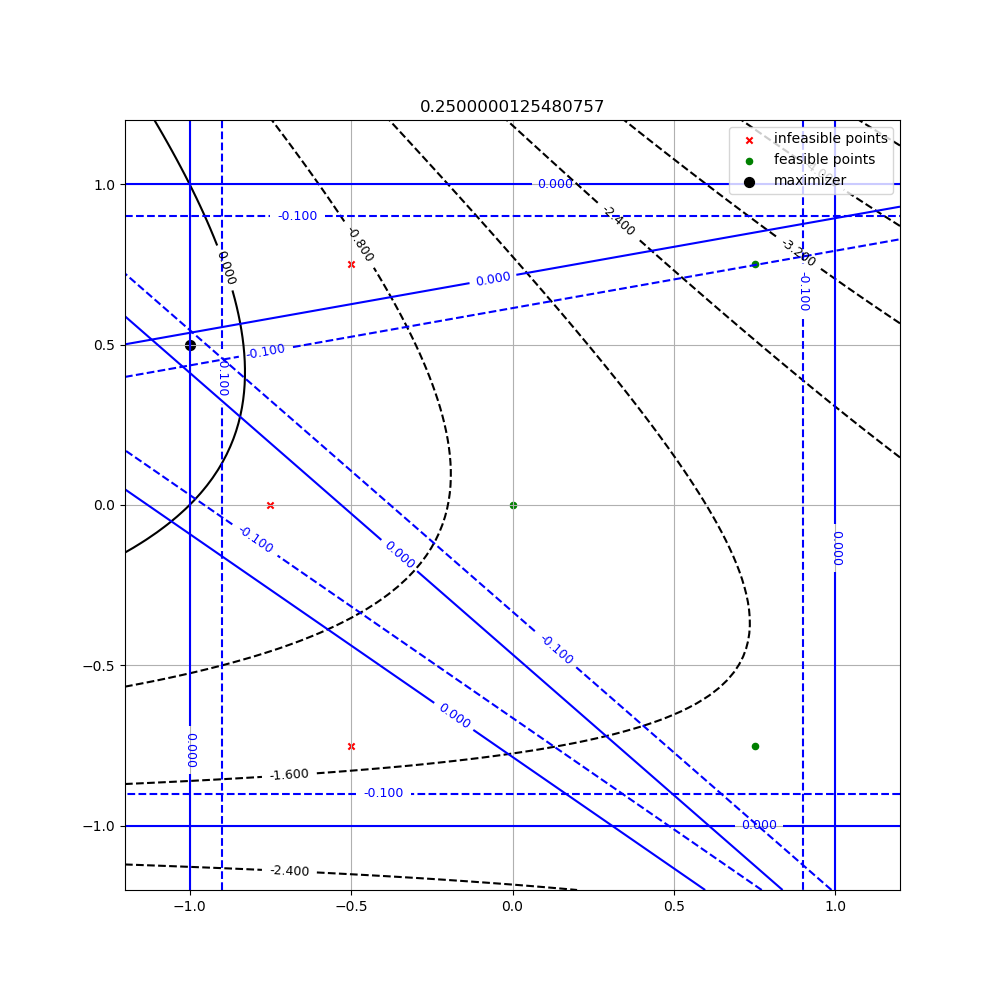
\includegraphics[width=300px]{images/pyomo_cut_solution.png}
    \caption{
		Adding linear cuts to remove infeasible points.
		Sample points that have already been evaluated and found to be feasible are shown as green circles.
		Attempted evaluations that resulted in infeasible evaluations are shown as red x's.
		The linear cuts (blue lines) are chosen to minimize the value of the objective (in black) while ensuring that all failed evaluations are infeasible.
	}
    \label{pvip}
\end{figure}


Suppose that the algorithm has evaluated several infeasible points after solving the trust region subproblem.
These are stored in a set $\trsinfset = \{n_1, n_2, \ldots, n_{|\trsinfset|}\}$.
We then choose one hyperplane $\{x \in \Rn | d_k^Tx = b_k\}$ for each infeasible point to remove that feasible point from our next attempt to solve the trust region subproblem.
Notice that these hyperplanes are \emph{decision variables} during the next attempt, so as to give as much freedom for our next trial solution.

If we let $\trstol \in (0, 1)$ be the percentage of the trust region radius with which we wish buffer our next solution, 
we arrive at the following optimization problem with $\searchtrk = \capcones \cap \tr $:
\begin{align}
\label{buffered_trust_region_subproblem}
\begin{array}{ccc}
\sk = \argmin_{s, d^{(k)} \in \Rn, b_i \in \reals}	& \mfk(x) & 	\\
 \mbox{subject to}  & n_k^Td^{(k)} \ge b_k + \trstol \dk& \forall k \in \left[ |\trsinfset |\right] \\
 & s^T d^{(k)} \le b_k &   \forall k \in \left[|\trsinfset |\right]  \\
 & \|d^{(k)}\| = 1 & \forall k \in \left[|\trsinfset |	\right]\\
 & \nabla \mcik(\xk) ^T s \le \mcik(\xk) & \forall i \in [m] \\
 & \|s - \xk \|_{\infty} \le \dk & \\
\end{array}
\end{align}

We use this optimization problem as a subroutine of the trust region subproblem algorithm:

\begin{algorithm}[H]
    \caption{Solve Trust Region Subproblem}
    \label{linear_cut_trust_region_subproblem}
    \begin{itemize}
        \item[\textbf{Step 0}] \textbf{(Initialization)} \\
	    Initialize the set of infeasible points $\trsinfset = \emptyset$.
        
        \item[\textbf{Step 1}] \textbf{Solve Trust Region Problem} \\
	    Solve \cref{buffered_trust_region_subproblem} to find trial point $s$.
	    If the feasible set is empty, \textbf{Fail}
        
        \item[\textbf{Step 2}] \textbf{(Check feasibility)} \\
            Evaluate the objective and constraints $s$. \\
            If $s\in\feasible$, \textbf{return} $s$.
            Otherwise, if $s\in\feasible$ and $s \in \sampletrk$, \textbf{Fail}
	    Otherwise, if $s\in\feasible$ and $s \not \in \sampletrk$ \begin{itemize}
	    	\item[] $\trsinfset \gets \trsinfset \cup \{s\}$
	    	\item[] Go to Step 1
	    \end{itemize}
            
        \item[\textbf{Step 3}] \textbf{(Update maximum volume ellipsoid)} \\
	    Update $E_{max}$
	    decrease random search variance
            
        $k \gets k+1$ and go to Step 1.
    \end{itemize}
\end{algorithm}

% The properties of the trial point found by this algorithm,
% as well as its convergence are detailed in \cref{efficiency_condition_analysis}.



\subsubsection{Decrease the Trust Region Radius}
\label{decreasing_the_trust_region_for_infeasible_trial}

Another option is to simply decrease the trust region radius.
However, in order to do this, we must be sure that we use a search region contained within $\feasible$ for small enough $\dk$.
In \cref{ellipsoid_is_feasible}, we show that the set $\capcones$ defined in \cref{define_capcones} is just this set.
Thus, we set $ \searchtrk = \capcones \cap \tr$ by defining the trust region subproblem as
\begin{align}
\label{capcones_tr_subproblem}
\begin{array}{ccc}
\min_{s^{(i)},x,t_i} & m_f(x) & \\
 & x = \wik + t _i s^{(i)} & \quad \forall i \in \activeconstraintsk \\
 & \|s^{(i)}\| = 1 & \quad \forall i \in \activeconstraintsk \\
 & -\left(s^{(i)}\right)^T\hgik \ge \beta \dk^{p_{\beta}} & \quad \forall i \in \activeconstraintsk \\
 & s^{(i)} \in \Rn  & \quad \forall i \in \activeconstraintsk \\
 & t_i > 0          & \quad \forall i \in \activeconstraintsk \\
 & x \in \tr		& \\
\end{array}
\end{align}
In \cref{sufficient_reduction_theorem} we show how to compute a point within $ \searchtrk $ that satisfies the efficiency condition \cref{efficiency}.


% \begin{comment}
% Double check that this is the same as in the masters2.tex
% \end{comment}

% The optimization program for finding this constraint is given by:
% 
% A set of $u^i, 1 \le i \le n_{I}$ infeasible points.
% A set of $v^i, 1 \le i \le n_{F}$ feasible points.
% 
% The current Lagrange polynomial $\frac 1 2 x^T Q x + b^Tx$.
% Require all infeasible point to be a distance at least $d$ from the feasible region.
% 
% 
% Find a set of planes $(n^i, b^i), 1 \le i \le n_{P}$.
% 
% Require $n_P \ge n_I$.
% 
% Let $n_I$ be the number of infeasible points
% Tolerance $\delta$
% \begin{align}
% \begin{array}{ccc}
% \min_{s, d_i \in \Rn, b_i \in \reals}	& \mfk(x) & 	\\
%  \mbox{subject to}  & d_k^T n_k \ge b_i + \trstol & \forall 1 \le k \le |\trsinfset | \\
%  & d_k^T s \le b_i &   \forall 1 \le k \le |\trsinfset |  \\
%  & \|d_k\| = 1 & \forall 1 \le k \le |\trsinfset |	\\
%  & \nabla \mcik(\xk) ^T s \le \mcik(\xk) & \forall i \in [m]\\
%  & \|s - \xk \|_{\infty} \le \dk & \\
% \end{array}
% \end{align}



\subsection{Recover Feasible Ellipsoid}

Although $\sampletrk$ will be feasible for small enough $\dk$, there may be some iterations in which it contains infeasible points.
When this happens, and a point we attempt to use as a sample point is infeasible, we decrease the trust region radius.
However, this means the previous sample points are no longer poised for the next iteration.
We then construct a feasible ellipsoid within the convex hull of the previous feasible points and the current iterate.

% \begin{algorithm}[H]
%     \caption{Restore a feasible ellipsoid}
%     \label{restore_feasible_ellipsoid}
%     \begin{itemize}
%         \item[\textbf{Step 0}] \textbf{(Initialization)} \\
%             Feasible ellipsoid, current iterate
%             
%         \item[\textbf{Step 1}] \textbf{(Construct Ellipsoid within the convex hull)} \\
%         	A sphere works.
%     \end{itemize}
% \end{algorithm}
% 
% \begin{comment}
% Fill this in.
% \end{comment}
% This is why we require an initial feasible ellipsoid.


To do this, we first construct the convex hull of the points 
Let $Y = y^{(0)}, y^{(1)}, \ldots, y^{(p)}$ be the set of sample points used in the previous iteration.

\begin{algorithm}[H]
    \caption{Restore a feasible ellipsoid}
    \label{restore_feasible_ellipsoid}
    \begin{itemize}
        \item[\textbf{Step 0}] \textbf{(Initialization)} \\
            $P_{\textrm{planes}} = \emptyset$
            
        \item[\textbf{Step 1}] \textbf{(Potentially add hyperplane)} \\
	    For each subset $S \subseteq Y \cup \{x^{(k-1)}\}$ with $|S| = n - 1$, construct the hyplerplane $ax\le b$ running through the points $S \cup \xk$.
	    If the inequality $ap \le b$ is valid for each $p \in Y \cup \{x^{(k-1)}\}$, add the pair $(a, b)$ to $P_{\textrm{planes}}$.
	
	\item[\textbf{Step 1}] \textbf{(Construct ellipsoid)} \\
	   Construct the largest possible ellipsoid within $P_{\textrm{planes}} \cap \tr$
    \end{itemize}
\end{algorithm}


\subsection{Convergent Algorithm}
\label{the_algroithm_section}

We can now state the algorithm.
The algorithm not only assumes the customary initial iterate $ \xinit $ with 
\begin{align}
\label{initial_point_is_feasible}
c\left(\xinit\right) < 0 \Longrightarrow \xinit \in \feasible.
\end{align}
but also an initial feasible ellipsoid
\begin{align}
\left\{x \in\Rn | \left(x - \xinit\right)^T Q^{(0)} \left(x - \xinit\right) \le \delta_0 \right\} \subseteq B_{\infty}\left(\xinit, \Delta_{0}\right) \cap \feasible \label{initial_ellipsoid}
\end{align}
to construct the first model.


\subsubsection{Pseudocode}
The algorithm is as follows:

\begin{algorithm}[H]
    \caption{Always-feasible Constrained Derivative Free Algorithm}	
    \label{constrained_dfo}
    \begin{itemize}
        \item[\textbf{Step 0}] \textbf{(Initialization)} \\
        	Initialize user supplied constants $\tolcrit, \tolrad$ by \cref{define_algorithm_tolerances};
        	$\gammasm$, $\gammabi$ by \cref{define_the_gammas};
        	$\omegadec$, $\omegainc$ by \cref{define_the_omegas};
        	$\alpha$, $\beta$, $p_{\alpha}$, and $p_{\beta}$ by \cref{define_abpab};
			$\kappa_{\chi}$ by \cref{define_kappa_chi};
			$\ximin$ by \cref{define_ximin};
			and $p_{\Delta}$ by \cref{define_p_delta}. \\
        	Initialize iteration counter: $k=0$, initial iterate $\xinit \in \feasible$, trust region radius $\Delta_0 > 0$, and feasible ellipsoid $T^{(0)}_{\textrm{interp}}$ as in \cref{initial_ellipsoid}.
            
        \item[\textbf{Step 1}] \textbf{(Construct the models)} \\
%         by \cref{define_ellipsek} if $\activeconstraintsk \ne \emptyset$ and \cref{define_trivial_ellipsek} if $\activeconstraintsk =\emptyset$.
        Call \cref{model_improving_algorithm} with respect to $\sampletrk$ to ensure the current sample set $Y^{(k)}$ satisfies \cref{accuracy}. \\
        Construct $\mfk$ and $\mcik$ as described in \cref{reg}.
        While constructing the sample set, if some point within $\sampletrk$ is not feasible, or $\sampletrk = \emptyset$ 
        run \cref{restore_feasible_ellipsoid} to construct a new $\sampletrk$ and $\dk$, and go to Step 1.
        
        \item[\textbf{Step 2}] \textbf{(Check stopping criteria)} \\
        	Compute $\activeconstraintsk$ by \cref{define_activeconstraints} and $\zik$, $\wik$ by \cref{define_z} and \cref{define_w} for each $i \in \activeconstraintsk$.
            Compute $\chi_k$ as in \cref{define_criticality_measure}. \begin{itemize}
                \item[] If $ \chik < \tau_{\xi} $ and $\dk <\tau_{\Delta}$ then return $\xk$ as the solution.
                \item[] Otherwise, if \cref{criticallity_check} is not satisfied, then \\
                $\Delta_{k+1} \gets \omegadec\dk$, 
                $x^{(k+1)} \gets \xk$,
                $k \gets k+1$ and go to Step 1.
            \end{itemize}
            
        \item[\textbf{Step 3}] \textbf{(Solve the trust region subproblem)} \\
        	Construct $\huk$, $\thetamink$, $\bsk$, $\fik$, and $\capcones$ according to
        	\cref{define_u}, \cref{define_thetamink}, \cref{define_bsk}, \cref{define_fik}, \cref{define_capcones}. \\
        	Use \cref{capcones_tr_subproblem} to compute the trial point $\sk$.
        	Evaluate the objective and constraints at $\sk$.
        	If $\sk \not \in \feasible$, reduce the trust region $\Delta_{k+1} = \omegadec\dk$, $k \gets k+1$ and go to Step 1.
            
        \item[\textbf{Step 4}] \textbf{(Test for improvement)} \\
            Evaluate $f(\xk + \sk)$ and evaluate $\rk$ as in \cref{define_rhok} \begin{itemize}
                \item[] If $\rk < \gammasm$ then $\xkpo=\xk$ (reject) and $\Delta_{k+1} = \omegadec\dk$
                \item[] If $\rk \ge \gammasm$ and $\rk < \gammabi$ then $\xkpo=\xk+\sk$ (accept), $\Delta_{k+1} = \omegadec\dk$
                \item[] If $\rk > \gammabi$ then $\xkpo=\xk+\sk$ (accept), $\Delta_{k+1} = \omegainc\dk$
                % and either increase the radius or decrease if $\nabla \mfk(\xk)$ is small
            \end{itemize}
            
        \item[\textbf{Step 5}] \textbf{(Construct next sample region)} \\
        	Compute $\rotk$, according to \cref{define_rotation}.
%         	Approximate $\activeconstraintskpo$ with $\approxactiveconstraintskpo$ defined by \cref{define_active_approximation} by checking if any $\zik \in B_{\infty}\left(\xkpo, \dkpo\right)$.
        	If $\activeconstraintskpo \ne \emptyset$, define $\sampletrkpo$ according to \cref{define_ellipsek}.
        	Otherwise, use \cref{define_trivial_ellipsek}. \\
            $k \gets k+1$ and go to Step 1.
    \end{itemize}
\end{algorithm}

\section{Convergence Analysis}
\label{convergence_discussion}
Within this section we show that \cref{constrained_dfo} converges to a critical point.
Our convergence analysis follows closely that of \cite{Conejo:2013:GCT:2620806.2621814}.
To use their analysis, we show that the accuracy and efficiency assumptions required for their proof hold, 
this is done within \cref{ellipsoidal_lambda} and \cref{sufficient_reduction_section} respectively.
Additionally, our criticallity measure defined by \cref{define_criticality_measure}:
$\chik = \left\|\xk - \text{Proj}_{\feasiblek}\left(\xk- \nabla \mfk\left(\xk\right)\right)\right\|$
depends on the current approximation of the constraints, which changes each iteration.
Thus, we must also show that the criticallity measure converges to the true criticallity measure
\begin{align}
\label{verbiage_hoffman_use_one}
\chik \approx \chi (\xk)
\end{align}
where 
\begin{align*}
\chi (x) = \left \| x - P_{\feasible}\left( x - \gradf\right) \right \|.
\end{align*}
For some results, we also show that the criticallity \cref{define_criticality_measure} measure converges across iterations:
\begin{align}
\label{verbiage_hoffman_use_two}
\chik \approx \chil.
\end{align}

We summarize the steps of the proof here:
\begin{itemize}
\item Show that the accuracy condition \cref{accuracy} is satisfied. \\
This is done within \cref{ellipsoidal_lambda}. 
To do this, we must show our construction of $\sampletrk$ satisfies the conditioned requirement defined by \cref{ellipsoids_notation_definitions}.
This is done within \cref{bounded_condition_numbers}.
\item Show that the efficiency condition \cref{efficiency} is satisfied. \\
This is the topic of \cref{sufficient_reduction_section}.
We use a slightly weaker efficiency condition, as stated in \cref{sufficient_reduction_theorem}.
\item Show $\liminf_{k\to\infty} \chik \to 0$. \\
This is done within \cref{initial_convergence_results}, and is a fairly straight forward use of the analysis within \cite{Conejo:2013:GCT:2620806.2621814}.
\item Show $\lim_{k\to\infty} \chik \to 0$ whenever $\gammabi > 0$. \\
This is done within \cref{limit_of_criticallity_to_zero}.
This result relies on \cref{verbiage_hoffman_use_one}, which in turn, depends on bounding the Hoffman constant of the constraint's model's Jacobians.
This is done within \cref{bounding_the_projection_section}.
This is complicated by the fact that we do not assume bounded level sets, so we do not have a gaurantee that the sequence $\left\{\xk\right\}$ is Cauchy.
Thus, we introduce \cref{criteria_from_contradiction}, which
\begin{itemize}
\item is sufficient to prove \cref{verbiage_hoffman_use_two},
\item follows from a false assumption within a proof of contradiction \cref{the_contradiction},
\item would be true under the stronger assumption of bounded level sets.
\end{itemize}
(For a discussion on simplifying the analysis with bounded level sets see \cref{bounded_level_sets}).
% \begin{itemize}
% \item This is one uses of the hoffman bound
% \item motivate criteria mention contradiction
% \end{itemize}
\item Show the limit of true criticallity measure is zero \\
This is done within \cref{limit_of_true_criticallity}.
This relies on \cref{verbiage_hoffman_use_two}, which in turn relies on bounding the Hoffman constant of the Jacobians of the constraints.
Because of the similarity, this is done in parallel with bounding the constraint's model's Jacobian's Hoffman's constant in \cref{bounding_the_projection_section}.
\end{itemize}

Throughout this section, we assume that 
$\left\{\xk\right\}$,
$\left\{\dk\right\}$,
$\left\{m_{c_i}\right\}$,
and
$\left\{m_{f}\right\}$
are generated by 
\cref{constrained_dfo}.
Other quantities such as $\activeconstraintsk$, $\huk$, $\thetamink$, $\qk$, $\ck$, and $\sdk$ 
that are generated by the conservative ellipsoid method described in
\cref{ellipsoid_requirements} and \cref{constructing_and_analysizing_conservative_ellipsoid}
include references to their definitions when used.


\subsection{Assumptions}
We will let $\Omega$ be some open region containing $\feasible$.

\begin{assumption}
\label{constraints_are_convex}
The functions $c_i$ for all $i \in [m]$ are convex in $ \Omega $. That is, 
% c_i(x) \le 0 \wedge c_i(y) \le 0 \Longrightarrow
\begin{align*}
c_i(\zeta x + (1 - \zeta) y) \le 0 \quad \forall x, y \in \Omega, \zeta \in [0, 1].
\end{align*}
\end{assumption}

% \paragraph{Bounded functions}
% The following assumptions let us know that the functions $f$ and $c_i$ for each $i \in [m]$ are bounded functions.

\begin{assumption}
\label{bounded_below_assumption}
The function $f$ is bounded below in $ \Omega $. That is, there exists $\fmin \in \reals$ such that
\begin{align*}
f(x) \ge \fmin \quad  \forall x \in \Omega.
\end{align*}
\end{assumption}

\begin{assumption}
\label{maximum_constraint_value_lemma}
% Suppose that \cref{constraints_are_convex}, \cref{bounded_hessians_assumption}, \cref{max_norm_assumption}, and \cref{lipschitz_gradients_assumption} hold.
The functions $c_i$ for $i \in [m]$ are bounded below in $ \Omega $.
That is, there exists $M_c>0$ such that
\begin{align*}
c_i(x) \ge -M_c \quad \forall i \in [m], x \in \Omega.
\end{align*}
\end{assumption}

\begin{assumption}
\label{bounded_gradients_lemma}
% Suppose \cref{max_norm_assumption} and \cref{lipschitz_gradients_assumption} hold.
The functions $f$ and $c_i$ for all $ i \in [m]$ have bounded gradient in $ \Omega $.
That is, there exists $\maxgrad > 0$ such that
\begin{align*}
\|\gradf(x)\| \le \maxgrad \quad  \forall x \in \Omega \\
\|\nabla c_i(x)\| \le \maxgrad \quad  \forall x \in \Omega, \quad \forall i \in [m].
\end{align*}
\end{assumption}

\begin{assumption}
\label{bounded_hessians_assumption}
Each function $c_i$ for $i \in [m]$ and $f$ has bounded Hessian. That is, there exists $ \maxhessian > 0$ such that:
\begin{align*}
\|\nabla^2 f(x) \| \le \maxhessian \quad \forall x \in \Omega \\
\|\nabla^2 c_i(x) \| \le \maxhessian \quad \forall x \in \Omega, \forall i \in [m]
\end{align*}
\end{assumption}

% \begin{assumption}
% \label{bounded_objective_hessians_assumption}
% The matrices $\hk$ are uniformly bounded, that is, there exists a constant $ \maxhessian \ge 1 $ such that 
% \begin{align}
% \|\hk\| \le \maxhessian \quad \forall k \ge 0.
% \end{align}
% \end{assumption}

% \color{red}
% We believe that the following assumption is stronger than required.
% This assumption is used while bounding differences in criticality measure across iterations, 
% so that it we would likely only need the intersection of $\feasiblek$ and the half space of vectors whose dot product with the negative gradient of the objective is positive to be bounded.
% \begin{assumption}
% \label{max_norm_assumption}
% The set $\feasible$ is bounded. That is, there exists $\maxnorm > 0$ such that
% \begin{align*}
% \|x\| \le \maxnorm \quad \forall x \in \feasible.
% \end{align*}
% \end{assumption}
% \color{black}


% \paragraph{All functions are smooth}
% The following assumptions let us know that the functions $f$ and $c_i$ for each $i \in [m]$ are smooth functions.

\begin{assumption}
\label{lipschitz_gradients_assumption}
The functions $c_i$ for all $i \in [m]$ and $f$ are differentiable and their gradients are Lipschitz continuous with constant $\lipgrad > 0$ in $ \Omega $:
\begin{align*}
\|\gradf(x) - \gradf(y)\| \le \lipgrad \|x - y\| \quad \forall x,y \in \Omega, \\
\|\nabla c_i(x) - \nabla c_i(y)\| \le \lipgrad \|x - y\| \quad \forall x,y \in \Omega, \forall i \in [m].
\end{align*}
\end{assumption}


\begin{assumption}
\label{lipschitz_hessians_assumption}
The functions $c_i$ for all $i \in [m]$ and $f$ are twice differentiable and their Hessians are Lipschitz continuous with constant $\liphess > 0$ in $ \Omega $:
\begin{align*}
\|\nabla^2 f(x) - \nabla^2 f(y)\| \le \liphess \|x - y\| \quad \forall x,y \in \Omega, \\
\|\nabla^2 c_i(x) - \nabla^2 c_i(y)\| \le \liphess \|x - y\| \quad \forall x,y \in \Omega, \forall i \in [m] .
\end{align*}
\end{assumption}


\paragraph{Regularity Assumptions}

% We use the following assumptions as our regularity assumptions.

The following was inspired by the Mangasarian Fromovitz constraint qualifications with only inequality constraints.
It provides a uniform bound across all points, rather than at just a critical point.

% For an alternative to this assumption, please see \cref{alternative_assumptions_section}.
% 
% \color{red}
% \begin{assumption}
% \label{minangleassumption}
% Define $\activeconstraintsk$ by \cref{define_activeconstraints}.
% There exists $\minangledelta > 0$ and $\minanglealpha > 0$ such that for each $k \in \naturals$ with $\dk \le \minangledelta$ there exists
% a unit vector $\minangledirk \in \Rn$
% such that
% \begin{align*}
% -\frac {\gmcik}{\left\|\gmcik\right\|} ^T\minangledirk \ge \minanglealpha \quad \forall i \in \activeconstraintsk.
% \end{align*}
% Without loss of generality, $\minanglealpha \le \frac 1 2$.
% \end{assumption}
% \color{black}

Remember that $\zik$ is defined by \cref{define_z}.
\begin{assumption}
\label{minangleassumption_alt}
There exists $\minangledelta > 0$ and $\minanglealpha > 0$ such that for each $k \in \naturals$ there exists
a unit vector $\minangledirk \in \Rn$
such that if $\dk \le \minangledelta$ and
$i$ is such that $\zik \in B_{\infty}(\xk, \minangledelta)$
then
\begin{align*}
-\frac {\gmcik}{\left\|\gmcik\right\|} ^T\minangledirk \ge \minanglealpha.
\end{align*}
Without loss of generality, $\minanglealpha \le \frac 1 2$.
\end{assumption}



\begin{assumption}
\label{mingradassumption}
There exist $\mingradepsilon > 0$ and $\mingrad > 0$ such that for each $x \in \Omega$, if $\left|c_i(x)\right| \le \mingradepsilon$, then
\begin{align*}
\| \nabla c_i(x) \| \ge \mingrad.
\end{align*}
% \| \nabla c_i(x) \| \ge \mingrad \quad \forall i \in \epsactive(x; \mingradepsilon).
\end{assumption}







% \paragraph{}
% 
% 
% \begin{lemma}
% Suppose that \cref{minangleassumption_alt} holds.
% If $\dk \le \Delta_{\textrm{a}}$, then
% \end{lemma}
% \begin{proof}
% 
% By \cref{minangleassumption_alt}, there exists an $\epsilon > 0$ and a $\minanglealpha$ such that for any $i \in \epsactive(x; \epsilon)$, we have
% \begin{align*}
% \nabla c_i(x)^T\minanglediralt(x) > \minanglealpha.
% \end{align*}
% Suppose that 
% 
% \begin{align*}
% \kappa_g \dk^2 \le \minanglealpha
% \end{align*}
% 
% \begin{align*}
% \minanglealpha < \nabla c_i(x)^T\minanglediralt(x) =
% \left(\nabla \mcik(x) + \kappa_g \dk^2 \sqrt{\sigma_{\textrm{max}}}\nu\right)^T\minanglediralt(x) \\
% \minanglealpha - \kappa_g \dk^2 \sqrt{\sigma_{\textrm{max}}}\nu^T\minanglediralt(x) < \nabla \mcik(x)^T\minanglediralt(x) \\ 
% \minanglealpha\left(1 - \sqrt{\sigma_{\textrm{max}}}\right) < \nabla \mcik(x)^T\minanglediralt(x) \\ 
% \end{align*}
% 
% \begin{align*}
% \nabla c_i(x) =  \\
% \dk \le \Delta_{\textrm{a}}
% \end{align*}
% 
% Suppose that $i \in \epsactive(x; \epsilon)$.
% Then, 
% Then there e
% 
% There exists a unit vector $\nu \in \Rn$, with $0 \le \|\nu\| \le 1$ such that 
% 
% 
% 
% \begin{align*}
% \nabla c_i(x)^T\minanglediralt(x) > \minanglealpha\quad \forall i \in  \\
% \nabla c_i(x) = \nabla \mcik(x) + \kappa_g \dk^2 \sqrt{\sigma_{\textrm{max}}}\nu \\
% \dk \le \Delta_{\textrm{a}}
% \end{align*}
% 
% \end{proof}




% \paragraph{Simple Theorems}

% \begin{proof}
% \begin{comment}
% The result follows from these being continuous functions over compact sets.
% \end{comment}
% 
% We are given a $\xinit \in \feasible$. Let $\maxgrad = 2\lipgrad \maxnorm + \max\left\{|\gradf\left(\xinit\right)|, \max_{i \in [m]}\left\{\nabla c_i\left(\xinit\right)|\right\} \right\}$.
% Thus, for any $x \in \Omega$,
% \begin{align*}
% \gradf(x) \le \left|\gradf\left(\xinit\right)\right| + \lipgrad \left\|x - 0 - \left(\xinit - 0\right)\right\| \le \left|\gradf\left(\xinit\right)\right| + 2\lipgrad \maxnorm \le \maxgrad.
% \end{align*}
% The same applies to each $c_i$.
% \end{proof}


% \begin{proof}
% \begin{comment}
% The result follows from these being continuous functions over compact sets.
% \end{comment}
% 
% Let $M_c = -c_i\left(\xinit\right) + \maxgrad\maxnorm + \maxhessian \maxnorm^2$.
% Because $\xinit \in\feasible$, $M_c > 0$.
% But, for all $i \in [m]$ and all $x \in \feasible$ we have by 
% \cref{constraints_are_convex} and \cref{bounded_hessians_assumption}
% \begin{align*}
% c_i(x) \ge c_i\left(\xinit\right) + \left(\nabla c_i\left(\xinit\right)\right)^T\left(x - \xinit\right) - \maxhessian \left\|x - \xinit\right\|^2
% \end{align*}
% and by \cref{bounded_gradients_lemma}, and \cref{max_norm_assumption}
% \begin{align*}
% c_i(x) \ge c_i\left(\xinit\right) - \maxgrad\maxnorm - \maxhessian \maxnorm^2 = -M_c.
% \end{align*}
% \end{proof}



\subsection{Bounded Condition Numbers}
\label{bounded_condition_numbers}
In this section, we show that the condition numbers $\sigma(\qk)$ are bounded.
This is required to show the accuracy condition \cref{accuracy}, because this condition number determines the sample sets poisedness, as discussed in \cref{geometry}.
% The accuracy condition dependThis condition number influences model's accuracy. 

\begin{lemma}
\label{theta_min_is_bounded}
Let $\minangledelta$ and $\minanglealpha$ be defined by \cref{minangleassumption_alt}, and
define $\thetamink$ by \cref{define_thetamink}.
Suppose that \cref{minangleassumption_alt} holds.
% Let $\minanglealpha$ and $\minangledelta$ be defined by \cref{minangleassumption} and 
If $\dk \le \minangledelta$, then $\thetamink \ge \minanglealpha$.
\end{lemma}

\begin{proof}
Let $\activeconstraintsk$ be defined by \cref{define_activeconstraints}.
If $\activeconstraintsk = \emptyset$, then $\thetamink = 1$.
Otherwise, by \cref{minangleassumption_alt}, there is a $\minangledirk$ such that 
$-\minangledirk^T\frac{\gmcik}{\|\gmcik\|} \ge \minanglealpha$ for any $i \in \activeconstraintsk$.
But, by definition of $\huk$ in \cref{define_u}:
$\huk = -\argmin_{\|u\| = 1} \max_{i \in \activeconstraintsk} u^T\frac{\gmcik}{\left\|\gmcik\right\|}$
so that for all $i \in \activeconstraintsk$,
\begin{align*}
-\left(\huk\right)^T\frac{\gmcik}{\|\gmcik\|}  \ge -\left(\minangledirk\right)^T\frac{\gmcik}{\|\gmcik\|} \ge \minanglealpha.
\end{align*}
Therefore, $\thetamink \ge \minanglealpha$.
\end{proof}

\begin{lemma}
\label{bounded_condition_numbers}
Let $\activeconstraintsk$ be defined by \cref{define_activeconstraints};
$\qkpo$ be defined by \cref{define_trivial_ellipsek} when $\activeconstraintsk = \emptyset$ and \cref{conservative_ellipsoid_details} otherwise;
and $\minanglealpha$ be defined by \cref{minangleassumption_alt}.
Suppose that \cref{minangleassumption_alt} holds.
% Then the sequence $\left(\qk, \ck, \sk\right)$ is conditioned as defined by \cref{ellipsoids_notation_definitions}.
There exists a $\dacc > 0$, such that $\sigma(\qkpo) \le {12}\left(\minanglealpha\right)^{-2}$ whenever $\dk \le \dacc$.
\end{lemma}
\begin{proof}
If $\activeconstraintsk = \emptyset$, then 
% \cref{define_suitable_condition_numbers} is satisfied because 
$\sigma\left(\qkpo\right) = 1$.
If $\activeconstraintsk \ne \emptyset$, then result follows directly from \cref{theta_min_is_bounded} and \cref{boundbeta} by letting
\begin{align}
\dacc = \min\left\{\minangledelta, \frac 1 {4 \beta} \left(\minanglealpha \right)^2 \right\} \label{define_delta_accuracy}
\end{align}
where $\minangledelta$ is defined by \cref{minangleassumption_alt}.
\end{proof}


\begin{lemma}
\label{sampletrk_is_nonempty}
Let $\dacc$ and $\fcki$ be defined by \cref{define_delta_accuracy} and \cref{define_inner_cone}.
Suppose that \cref{minangleassumption_alt} holds.
If $\dk \le \dacc$, then the tuple $(\qk, \ck, \sdk)$ defined in \cref{define_ellipsek}
is non-empty according to \cref{ellipsoids_notation_definitions}, and $\fcki \ne \emptyset$.
\end{lemma}
\begin{proof}
Let $\minanglealpha$ be defined by \cref{minangleassumption_alt}.
\cref{theta_min_is_bounded} and \cref{boundbsk} tell us that 
if $\dk \le \dacc$, then $\thetamink \ge \minanglealpha$, 
so that the definitions \cref{define_bsk} and \cref{define_bs} imply
$\bsk < 1 \Longrightarrow \frac{\bsk}{1 - \bsk} > 0$.
Thus, the set of directions in \cref{define_inner_cone} is non empty, and
$\fcki \ne \emptyset$.
\end{proof}


\subsection{Accuracy}
\label{ellipsoidal_lambda}

% We will be using the following result shown in \cite{BillupsLarson2013}, Corollary 4.7.
% We restate the theorem here, with the simplication that $f$ is deterministic function.
% Note that the assumptions are satisfied by .
We also use the following two theorems found within our convergence analysis for linear constraints:

\begin{lemma}
\label{change_radius} 
Suppose that \cref{bounded_hessians_assumption} and \cref{lipschitz_gradients_assumption} hold.
Assume that $f$ is twice continuously differentiable with bounded and Lipschitz continuous Hessian in $\Omega$ with bound $M$ and Lipschitz constant $\liphess$.
% Let $Y$ be a poised set of $p + 1$ points, and let $R = \max_{i}\|y^i - y^0\|$.
% Let $m_f(x)$ denote the quadratic model of $f$ using \cref{reg}.
Suppose there there exist constants $\Lambda_1, \Lambda_2, \Lambda_3$ such that for all $x \in B\left(y^0, \Delta\right)$,
\begin{align*}
\left|f(x) - m_f(x)\right| \le \Lambda_1 \\ % \Delta^3
\left\|\gradf(x) - \nabla m_f(x)\right\| \le \Lambda_2 \\ % \Delta^2
\left\|\nabla^2 f(x) - \nabla^2 m_f(x)\right\| \le \Lambda_3. % \Delta
\end{align*}
Then let $r > 1$ be arbitrary.
There exist constants $\Lambda_1', \Lambda_2', \Lambda_3'$ such that for all $x \in B\left(y^0, r\Delta\right)$,
\begin{align*}
\left|f(x) - m_f(x)\right| \le \Lambda_1' r^2 \\ % \Delta^3
\left\|\gradf(x) - \nabla m_f(x)\right\| \le \Lambda_2' r\\ % \Delta^2
\left\|\nabla^2 f(x) - \nabla^2 m_f(x)\right\| \le \Lambda_3' r .% \Delta
\end{align*}
\end{lemma}

\begin{proof}
Let $x \in B\left(y^{0}, r\Delta\right)$, and define
\begin{align*}
\Lambda_3' = \Lambda_3 + \liphess \Delta \\
\Lambda_2' = 2 \Delta M + \Lambda_2 +  \Delta \Lambda_3'\\
\Lambda_1' = \Lambda_1 + \Lambda_2' \Delta\\
\end{align*}
First, note that because $m_f$ is a quadratic model,
\begin{align*}
\left\| \nabla^2 f\left(x\right) - \nabla^2 m_f\left(x\right)\right\|
= \left\| \nabla^2 f\left(x\right) - \nabla^2 m_f\left(y^0\right)\right\|
\le \left\| \nabla^2 f\left(x\right) - \nabla^2 f\left(y^0\right)\right\| + \left\| \nabla^2 f\left(y^0\right) - \nabla^2 m_f\left(y^0\right)\right\| \\
\le \liphess \|x - y\| + \Lambda_3 \le  \Lambda_3' r .
\end{align*}


By the mean value theorem, there exists $\xi^1 \in [y^0, x]$ with
\begin{align*}
\left\|\nabla f(x) - \nabla f\left(y^0\right) \right\|
\le \left\|x - y^0\right\| \left\| \nabla^2 f\left(\xi^1\right) \right\|
\le r \Delta M \\
\left\|\nabla m_f(x) - \nabla m_f\left(y^0\right) \right\|
\le \left\|x - y^0\right\| \left\| \nabla^2 m_f\left(y^0\right) \right\|
\le r \Delta \left(M + \Lambda_3'\right)
\end{align*}
Thus,
\begin{align*}
\left\|\nabla f(x) - \nabla m_f(x)\right\| \le 
\left\| \nabla f(x) - \nabla f(y^0) \right\| + \left\|\nabla f(y^0) - \nabla m_f(y^0)\right\| + \left\|\nabla m_f(y^0) - \nabla m_f(x)\right\| \\
\le r \Delta M + \Lambda_2 + r \Delta \left(M + \Lambda_3'\right)
\le r \left(2 \Delta M + \Lambda_2 +  \Delta \Lambda_3'\right)
\le r \Lambda_2'.
\end{align*}

Finally, by the mean value theorem, there is a $\xi^2 \in [y^0, x]$ with
\begin{align*}
\left|f(x) - m_f(x)\right|
\le \left| f(y^0) - m_f(y^0) \right| + \left\| \nabla f(\xi^2) - \nabla f(\xi^2) \right\| \left\|x - y^0\right\|
\le \Lambda_1 + \Lambda_2' \Delta r^2
\le \Lambda_1' r^2.
\end{align*}
% 
% 
% 
% \begin{align*}
% \left| f(x) -  f\left(y^0\right) \right|
% \le \left\|x - y^0\right\| \left\| \nabla f\left(\xi\right) \right\|
% \le r \Delta \liphess \\
% \left\|\nabla m_f(x) - \nabla m_f\left(y^0\right) \right\|
% \le \left\|x - y^0\right\| \left\| \nabla^2 m_f\left(y^0\right) \right\|
% \le r \Delta \left(\liphess + \Lambda_3'\right)
% \end{align*}
% Thus,
% \begin{align*}
% \left\|\nabla f(x) - \nabla m_f(x)\right\| \le 
% \left\| \nabla f(x) - \nabla f(y^0) \right\| + \left\|\nabla f(y^0) - \nabla m_f(y^0)\right\| + \left\|\nabla m_f(y^0) - \nabla m_f(x)\right\| \\
% \le r \Delta \liphess + \Lambda_2 + r \Delta \left(\liphess + \Lambda_3'\right)
% \le r \left(2 \Delta \liphess + \Lambda_2 +  \Delta \Lambda_3'\right)
% \le r \Lambda_2'.
% \end{align*} 
% 
% 
% Define $z = y^0 + \Delta\frac{x - y^0}{\left\|x - y^0\right\|}$, and notice $z \in B_{\infty}\left(y^0, \Delta\right)$.
% 
% 
% 
% Subtracting this from
% \begin{align*}
% m_f(x) = m_f\left(y^0\right) + \nabla m_f\left(y^0\right)^T\left(x - y^0\right) + (x - y^0)^T\nabla^2 m_f(y^0) (x - y^0),
% \end{align*}
% 
% 
% 
% and define $z = y^0 + \Delta\frac{x - y^0}{\left\|x - y^0\right\|}$.
% Because $z \in B\left(y^0, \Delta\right)$, we know that
% 
% \begin{align*}
% \left|f(z) - m_f(z)\right| \le \Lambda_1 \\ % \Delta^3
% \left\|\gradf(z) - \nabla m(z)\right\| \le \Lambda_2 \\ % \Delta^2
% \left\|\nabla^2 f(z) - \nabla^2 m(z)\right\| \le \Lambda_3 % \Delta
% \end{align*}
% and that there exists 
% % $\alpha \in [0, 1]$, 
% $\chi_1 \in [y^0, x]$ and
% $\chi_2 \in [z, x]$
% such that such that
% \begin{align*}
% f(x) &= f(y^0) + \nabla f\left(y^0\right)^T(x - y^0) + \left(x - y^0\right)^T\nabla^2 f (\chi_1)\left(x - y^0\right) \\
% f(x) &= f(z) + \nabla f\left(z\right)^T(x - z) + \left(x - z\right)^T \nabla^2 f (\chi_2)\left(x - z\right) \\
% m_f(x) &= m_f\left(y^0\right) + \nabla m_f\left(y^0\right)^T\left(x - y^0\right) + \left(x - y^0\right)^T\nabla^2 m_f\left(y^0\right)\left(x - y^0\right)
% \end{align*}
% we have
% \begin{align*}
% f(x) - m_f(x) = f\left(y^0\right) - m_f\left(y^0\right) 
% + \left[\nabla f\left(y^0\right) - \nabla m_f\left(y^0\right)\right]^T\left(x - y^0\right) \\
% + \left(z - y^0\right)^T\left[\nabla^2 f(\chi_1) - \nabla^2 m_f(y^0)\right]\left(z - y^0\right) \\
% \left|f(x) - m_f(x)\right| 
% \le \left|f\left(y^0\right) - m_f\left(y^0\right)\right|
% + \left\|\nabla f\left(y^0\right) - \nabla m_f\left(y^0\right)\right\| \|
% \end{align*}
% 
% 
% 
% \begin{align*}
% \left\| \nabla^2 f\left(x\right) - \nabla^2 m_f\left(x\right) \right\| \\
% = \left\| \nabla^2 f\left(x\right) - \nabla^2 f\left(y\right) \right\| 
% + \left\| \nabla^2 f\left(y\right) - \nabla^2 m_f\left(y\right) \right\|
% + \left\| \nabla^2 m_f\left(y\right) - \nabla^2 m_f\left(x\right) \right\| \\
% \le \liphess \left\|x - y \right\| + \Lambda_2 + 
% \end{align*}
% 
% 
% 
% \begin{align*}
% \nabla^2 f\left(x\right) \le \nabla^2 f\left(y^0\right) + \liphess \|x - y\| \\
% \left\| \nabla^2 f\left(x\right) - \nabla^2 f\left(y^0\right)\right\| \le \liphess \|x - y\| \\
% \left\| \nabla^2 f\left(x\right) - \nabla^2 m_f\left(y^0\right)\right\| + \left\| \nabla^2 m_f\left(y^0\right) - \nabla^2 f\left(y^0\right)\right\| \le \liphess \|x - y\| \\
% \left\| \nabla^2 f\left(x\right) - \nabla^2 m_f\left(y^0\right)\right\| \le \liphess r + \Lambda_3 \le \left(\liphess + \Lambda_3\right) r \\
% \end{align*}
% 
% 
% 
% 
% \begin{align*}
% \phi_i\left(x\right) = \phi_i\left(y\right) + 
% \end{align*}
% 
% 
% 


\end{proof}


\begin{theorem}
\label{shifted_ellipsoid}
Let a positive-definite, symmetric $n\times n$ matrix $\qk$, a vector $\ck \in \Rn$, and constant $\sdk$ be given.
Let $\qk = L D^2 L^T$ be the eigen-decomposition of $\qk$ where $L^TL = I$ and $D$ is a diagonal matrix with positive entries.
Also, let $\delta = \max_{x\in \unshiftedellipsoid}\|x-\ck\|$, 
and define the transformation $T(x) = \delta DL^T(x - \ck)$.
Let $\hat m_f(u)$ be a model of the shifted objective $\hat f(u) = f(T^{-1}(u))$ in the $\delta$ ball such that
there exist constants $\kappa_{ef}, \kappa_{eg}, \kappa_{eh} > 0$ such that for all $\{u \in R^n | \;\|u\| \le \delta \}$, we have
% for all $u \in B(0 ; \delta)$ we have the following error bounds:
\begin{align*}
|\hat m_f(u) - \hat f(u)| \le \kappa_{ef} \delta^3\\
\|\nabla \hat m_f(u) - \nabla \hat f(u)\| \le \kappa_{eg}\delta^2\\
\|\nabla^2 \hat m_f(u) - \nabla^2 \hat f(u)\| \le \kappa_{eh}\delta.
\end{align*}

Then, with
\begin{align*}
\kappa_{ef}' = \kappa_{ef} \\
\kappa_{eg}' = \kappa_{eg}\sqrt{\sigma(\qk)} \\
\kappa_{eh}' = \kappa_{eh}\sigma(\qk),
\end{align*}
we have that for all $x \in \unshiftedellipsoid$,
the model function $m_f(x) = \hat m_f(T(x))$ will satisfy
\begin{align*}
| m(x) - f(x)| \le \kappa_{ef}'\delta^3 \\
\|\nabla  m(x) - \nabla  f(x)\| \le \kappa_{eg}'\delta^2 \\
\|\nabla^2 m(x) - \nabla^2 f(x)\| \le \kappa_{eh}'\delta.
\end{align*}
\end{theorem}


\begin{lemma}
\label{accuracy_is_satisfied_lemma}
Fix an iterate $k$.
Suppose that $\qkmo$, $\ckmo$, and $\sdkmo$ are non-empty according to \cref{ellipsoids_notation_definitions}.
Suppose that \cref{bounded_hessians_assumption}, \cref{lipschitz_gradients_assumption} hold.
There exist $\kappa_g>0$ and $\kappa_h>0$ such that
\begin{align*}
\|\gradf(\xk) - \nabla \mfk(\xk) \| \le \kappa_g \sqrt{\sigma \left(\qkmo\right)} \dk^2, \\
\|\nabla^2 f(\xk) - \hk \| \le \kappa_h \sigma \left(\qkmo\right) \dk,  \\
\|\nabla c_i(\xk) - \gmcik \| \le \kappa_g \sqrt{\sigma \left(\qkmo\right)} \dk^2 \quad \forall i \in [m], \quad \textrm{and}\\
\|\nabla^2 c_i(\xk) - \nabla^2 m_{c_i}^{(k)}(\xk) \| \le \kappa_h \sigma \left(\qkmo\right) \dk \quad \forall i \in [m]. \\
\end{align*}
\end{lemma}

\begin{proof}
Give $\qkmo = LD^2L^T$ its eigen-decomposition, and define $\delta = \max_{x \in \unshiftedellipsoid} \|x - \ckmo\|$, as in \cref{shifted_ellipsoid}.
Then the transformation $T(x) = \delta D L^T(x - \ckmo)$ maps $\unshiftedellipsoid$ to the $\delta$ ball.
As also described in \cref{shifted_ellipsoid}, we create transformed functions
\begin{align*}
\begin{array}{ccc}
\hat {m}_f(u) = m_f(T^{-1}(u)),&  \hat f (u) = f(T^{-1}(u)) &\\
\hat {m}_{c_i}(u) = m_{c_i}(T^{-1}(u)), &  \hat c_i (u) = c(T^{-1}(u))& \forall i \in [m]
\end{array}
\end{align*}
After using \cref{model_improving_algorithm} to choose sample points, we know by \cref{quadratic_errors} that
there exist constants $\kappa_f, \kappa_g, \kappa_h$ such that for all $u \in B_2(0, \delta)$ and all $i \in [m]$:
\begin{align*}
\begin{array}{ccc}
\left\| \hat {f}\left(u\right) -  \hat{m}_f\left(u\right) \right\|\le \kappa_f \delta^3 &
\left\|\nabla \hat {f}\left(u\right) - \nabla \hat{m}_f\left(u\right) \right\|\le \kappa_g \delta^2 &
\left\|\nabla^2 \hat {f}\left(u\right) - \nabla^2 \hat{m}_f\left(u\right) \right\|\le \kappa_h \delta \\
\left\| \hat {{c_i}}\left(u\right) -  \hat{m}_{c_i}\left(u\right) \right\|\le \kappa_f \delta^3 &
\left\|\nabla \hat {{c_i}}\left(u\right) - \nabla \hat{m}_{c_i}\left(u\right) \right\|\le \kappa_g \delta^2 &
\left\|\nabla^2 \hat {{c_i}}\left(u\right) - \nabla^2 \hat{m}_{c_i}\left(u\right) \right\|\le \kappa_h \delta.
\end{array}
\end{align*}
By \cref{change_radius}, there are constants $\Lambda_2, \Lambda_3$ such that for all $u \in B_2(0, 2\delta)$ and $i \in [m]$:
\begin{align*}
\begin{array}{cc}
\left\|\nabla \hat {f}\left(u\right) - \nabla \hat{m}_f\left(u\right) \right\|\le 2\Lambda_2 \delta^2 = {\kappa'}_g\delta^2, &
\left\|\nabla \hat {c_i}\left(u\right) - \nabla \hat{m}_{c_i}\left(u\right) \right\|\le {\kappa'}_g\delta^2 \\
\left\|\nabla^2 \hat {f}\left(u\right) - \nabla^2 \hat{m}_f\left(u\right) \right\|\le 2\Lambda_3 \delta = {\kappa'}_h\delta^2, &
\left\|\nabla^2 \hat {c_i}\left(u\right) - \nabla^2 \hat{m}_{c_i}\left(u\right) \right\|\le {\kappa'}_h\delta^2 \\
\end{array}
\end{align*}
where $\kappa_{g}' = 2 \Lambda_2$ and $\kappa_{h}' = 2\Lambda_3$.
% Define $\kappa''_{g} =  \sqrt{\sigmamax}\kappa'_g$ and $\kappa''_h = \sigmamax\kappa'_h$.
Notice that because $\sigma_{\textrm{min}} = 1$, we have that $\sigmamax = \sigma \left(\qk\right)$.
\cref{shifted_ellipsoid} tells us for all $x_0 \in \scaledunshiftedellipsoid$:
\begin{align*}
\left\|\gradf\left(x_0 \right) - \nabla m^{(k)}_f\left(x_0\right)\right\| \le 
\kappa'_g  \dk^2 \sqrt{\sigma\left(\frac 2 {\sdk} \qkmo\right)} \le \kappa'_g \sqrt{\sigma\left(\qkmo\right)}\dk^2 \\
\left\|\nabla {c_i}\left(x_0 \right) - \nabla m^{(k)}_{c_i}\left(x_0\right)\right\| \le \kappa'_g\sqrt{\sigma\left(\qkmo\right)} \dk^2 \quad \forall i \in [m] \\
\left\|\nabla^2\left(x_0 \right) - \nabla m^{(k)}_f\left(x_0\right)\right\| \le \kappa'_h\sigma\left(\qkmo\right)\dk, \\
\left\|\nabla^2 {c_i}\left(x_0 \right) - \nabla^2 m^{(k)}_{c_i}\left(x_0\right)\right\| \le \kappa'_h\sigma\left(\qkmo\right)\dk \quad \forall i \in [m]
\end{align*}
In particular, $\xk \in \scaledunshiftedellipsoid$.
\end{proof}


\begin{theorem}
\label{accuracy_is_satisfied}
Let $\activeconstraintsk$ and $\dacc$ be defined by \cref{define_activeconstraints}, and \cref{define_delta_accuracy}.
Also, let $\qk$, $\ck$, and $\sdk$ 
be as generated by \cref{constrained_dfo}.
Suppose that 
\cref{bounded_hessians_assumption}, \cref{lipschitz_gradients_assumption}, and \cref{minangleassumption_alt} hold.
There exist $\kappa_g>0$ and $\kappa_h>0$ such that
\begin{align*}
\begin{array}{ccc}
\|\gradf(\xk) - \nabla \mfk(\xk) \| \le \kappa_g \dk^2, & \|\nabla^2 f(\xk) - \hk \| \le \kappa_h \dk, & \\
\|\nabla c_i(\xk) - \gmcik \| \le \kappa_g \dk^2, & \|\nabla^2 c_i(\xk) - \nabla^2 m_{c_i}^{(k)}(\xk) \| \le \kappa_h \dk & \forall i \in [m]. \\
\end{array}
\end{align*}
whenever $\dk \le \dacc$.
\end{theorem}
\begin{proof}
This is a direct consequence of \cref{accuracy_is_satisfied_lemma}, \cref{ellsoid_is_suitable_theorem_p1}, and \cref{bounded_condition_numbers}.
\end{proof}

\begin{lemma}
\label{bounded_model_hessian_lemma}
Let $\dacc$ be defined by \cref{accuracy_is_satisfied}.
Suppose that \cref{bounded_hessians_assumption}, \cref{lipschitz_gradients_assumption}, and \cref{minangleassumption_alt} hold.
Then there exists a $\maxmodelhessian > 0$ such that 
\begin{align*}
\| \hk \| \le \maxmodelhessian \quad \forall x \in \feasible \\
\|\nabla^2 m_{c_i}^{(k)}(\xk) \| \le \maxmodelhessian \quad \forall x \in \feasible, \forall i \in [m]
\end{align*}
whenever $\dk \le \dacc$.
\end{lemma}

\begin{proof}
Let $\kappa_h$ and $\maxhessian$ be defined by \cref{accuracy_is_satisfied} and \cref{bounded_hessians_assumption} respectively,
and let $\maxmodelhessian = \maxhessian + \kappa_h \dacc$.
Then \cref{bounded_hessians_assumption} tells us that
$\|\nabla^2 f(\xk)\| \le \maxhessian$, so that by \cref{accuracy_is_satisfied},
$\|\hk\| \le \|\nabla^2 f(\xk)\| + \kappa_h\dacc = \maxmodelhessian$.
The same applies to each $\nabla^2 m_{c_i}^{(k)}(\xk)$.
\end{proof}

\begin{lemma}
\label{i_thought_i_proved_this_already}
Let $\dacc$ be defined by \cref{accuracy_is_satisfied}.
Suppose the assumptions for
\cref{bounded_gradients_lemma},
\cref{accuracy_is_satisfied}
hold.
There exists a $\maxmodelgrad$ such that for each $k \in \naturals$, 
\begin{align*}
\left\| \gk \right\| \le \maxmodelgrad \quad
\textrm{and} \quad \left\|\gmcik\right\| \le \maxmodelgrad \quad \forall i \in [m]
\end{align*}
whenever $\dk \le \dacc$.
Without loss of generality, we may assume that $\maxmodelgrad \ge 1$.
\end{lemma}
\begin{proof}
Let $\kappa_g$ and $\maxgrad$ be defined by \cref{accuracy_is_satisfied} and \cref{bounded_gradients_lemma} respectively,
and let $\maxmodelhessian = \maxgrad + \kappa_g \dacc^2$.
Using \cref{accuracy_is_satisfied} to define $\kappa_g$, we can let $\maxmodelgrad = \maxgrad + \kappa_g \dacc^2$.
Then \cref{bounded_gradients_lemma} tells us that
$\|\nabla f(\xk)\| \le \maxgrad$, so that by \cref{accuracy_is_satisfied},
$\|\hk\| \le \|\nabla f(\xk)\| + \kappa_g\dacc^2 = \maxmodelgrad$.
The same applies to each $\left\|\gmcik\right\|$.
\end{proof}

\subsection{Sample Region Feasibility}
\label{ellipsoid_is_feasible_section}

Within this section, we will show that the conservative ellipsoids defined by \cref{define_ellipsek} are feasible as defined by \cref{ellipsoids_notation_definitions}:
that is, $\sampletrk \subseteq \feasible$.
% In order to do this, we would first show 
% \begin{align*}
% c_i(y) \le 0 \quad \forall y \in \fik \cap \tr.
% \end{align*}
% During iteration $k$, we construct an ellipsoid that is meant to be feasible for 

\begin{lemma}
\label{only_small_z_matters}
Let $\zik$ and $\mingrad$ be defined by \cref{define_z} and \cref{mingradassumption} respectively.
Suppose that 
\cref{bounded_hessians_assumption},
\cref{lipschitz_gradients_assumption},
\cref{minangleassumption_alt},
and \cref{mingradassumption} hold.
There exists $\mingraddelta > 0$ such that if $\dk \le \mingraddelta$ then for all $i \in [m]$ either
\begin{itemize}
\item $c_i(y) \le 0 \quad \forall y \in \left[\tr \cup \trkpo\right]$ or
\item both $\zik \in \tr$ and $\left\|\gmcik\right\| > \frac 1 2 \mingrad$.
\end{itemize}
\end{lemma}
\begin{proof}
Fix an $i \in [m]$.
Let
$\dacc$,
$\maxgrad$,
$\omegainc$, 
and $\maxmodelhessian$
be defined by
\cref{define_delta_accuracy},
\cref{bounded_gradients_lemma},
\cref{define_the_omegas},
and \cref{bounded_model_hessian_lemma}
respectively.
By \cref{accuracy_is_satisfied}, there exists a $\kappa_g$ such that
\begin{align}
\label{oszm_accuracy}
\left\|\nabla c_i(x) - \gmcik\right\| \le \kappa_g \dk^2.
\end{align}
Define
\begin{align}
\dk \le \mingraddelta = \min\left\{
\dacc,
\sqrt{\frac 1 {2\kappa_g} \mingrad},
\sqrt{\frac 1 {2\kappa_g} \maxgrad},
\frac{\mingradepsilon}{\frac 3 2 \maxgrad\sqrt{n}\left(1 + \omegainc\right) + n \maxmodelhessian \left(1 + \omegainc\right)^2},
\sqrt{\frac{2\mingradepsilon}{\mingrad}}
\right\} \label{define_mingraddelta}
\end{align}
and let $y\in \left[\tr \cup \trkpo\right]$.
Notice that $\dkpo \le \omegainc \dk$ and $\left\|\xk - \xkpo\right\| \le \sqrt{n}\dk$ imply
\begin{align*}
\left\|y - \xk\right\| \le \left\|y - \xkpo\right\| + \left\|\xkpo - \xk\right\| \le \sqrt{n}\left(1 + \omegainc\right)\dk.
\end{align*}

By \cref{bounded_hessians_assumption}, we have
\begin{align}
c_i(y) \le c_i(\xk) + \left(\gmcik\right)^T(y - \xk) + \frac 1 2 \left(y - \xk\right)^T\nabla^2{c_i}(\xk)\left(y - \xk\right) \nonumber \\
\le c_i(\xk) + \left\|\gmcik\right\|\left(1 + \omegainc\right) \sqrt{n}\dk +n \left(1 + \omegainc\right)^2\maxmodelhessian\dk^2.
\label{oszm_first_bound}
\end{align}

\emph{Case 1}
Suppose that $-m_{c_i}(\xk) \ge \mingradepsilon \Longrightarrow -c_i(\xk) \ge \mingradepsilon$.
Using \cref{oszm_accuracy}, \cref{bounded_gradients_lemma} and 
$\dk \le \sqrt{\frac {\maxgrad} {2\kappa_g}} \Longrightarrow \kappa_g \dk^2 \le \frac 1 2 \maxgrad$ from \cref{define_mingraddelta} we have
\begin{align}
\label{oszm_second_bound}
\left\| \gmcik \right\| \le \left\|\nabla c_i(\xk)\right\| + \kappa_g \dk^2 \le \frac 3 2 \maxgrad.
\end{align}
Also from \cref{define_mingraddelta} we have
\begin{align*}
\left(\frac 3 2 \maxgrad\sqrt{n} \left(1 + \omegainc\right) + n \maxmodelhessian \left(1 + \omegainc\right)^2 \right)\dk \le \mingradepsilon
\end{align*}
and using $\dk \le 1$, we can multiply the second term in paranthesis by $\dk$:
\begin{align*}
\frac 3 2 \maxgrad\sqrt{n} \left(1 + \omegainc\right) \dk + n \maxmodelhessian \left(1 + \omegainc\right)^2\dk^2 \le \mingradepsilon.
\end{align*}
Substituting \cref{oszm_second_bound} into the first term and using our assumption $-c_i(\xk) \ge \mingradepsilon$, we see
\begin{align*}
\left\|\gmcik\right\|\sqrt{n}\left(1 + \omegainc\right) \dk + n \maxmodelhessian \left(1 + \omegainc\right)^2\dk^2  \le \mingradepsilon \le -c_i(\xk).
\end{align*}
Adding $c_i(\xk)$ to both sides yields
\begin{align*}
c_i(\xk) + \left\|\gmcik\right\|\sqrt{n}\left(1 + \omegainc\right) \dk + n \left(1 + \omegainc\right)^2\maxmodelhessian\dk^2 \le 0.
\end{align*}
Combine this with \cref{oszm_first_bound} to see that $c(y) \le 0$.


\emph{Case 2}
Suppose that $-m_{c_i}(\xk) \le \mingradepsilon \Longrightarrow -c_i(\xk) \le \mingradepsilon$.
Then, by \cref{mingradassumption}, 
$\left\|\nabla c(\xk) \right\| \ge \mingrad$.
Using \cref{oszm_accuracy} and \cref{define_mingraddelta}, this implies
$\|\gmcik\| \ge \mingrad - \kappa_g \dk^2 \ge \frac 1 2 \mingrad > 0$.
Continuing with \cref{define_z}, \cref{define_mingraddelta}, and $\dk \le 1$ we find
\begin{align*}
\|\zik-\xk\| = \frac{-c\left(\xk\right)}{\left\|\gmcik\right\|} \le \frac{2\mingradepsilon}{\mingrad}\le \dk^2 \le \dk \Longrightarrow \zik \in \tr.
\end{align*}
\end{proof}

\begin{lemma}
\label{each_constraints_cone_is_feasible}
Let $\fik$ be defined by \cref{define_fik}.
Suppose that 
\cref{bounded_hessians_assumption},
\cref{lipschitz_gradients_assumption},
\cref{minangleassumption_alt},
and \cref{mingradassumption} hold.
There exists $\dfeas > 0$ such that
if $\dk \le \dfeas$, then
\begin{align*}
c_i(y) \le 0 \quad \forall y \in \fik \cap \left[\tr \cup \trkpo\right].
\end{align*}
\end{lemma}

\begin{proof}
Let
$\alpha$, $\beta$, $p_{\alpha}$, and $p_{\beta}$
be defined by
\cref{define_abpab},
and let
$\omegainc$,
$\mingraddelta$,
$\maxhessian$
$\lipgrad$
and $\mingrad$
be defined as in
\cref{define_the_omegas},
\cref{define_mingraddelta},
\cref{bounded_hessians_assumption},
\cref{lipschitz_gradients_assumption},
and \cref{mingradassumption}
respectively.

By \cref{accuracy_is_satisfied}, there exist $\kappa_g > 0$ and $u\in\Rn$ with $\|u\|\le 1$ such that:
\begin{align}
\nabla c_i(\xk) = \nabla m_{c_i}(\xk) + \kappa_g\dk^2 u. \label{model_error_for_gradient}
\end{align}

We define
\begin{align}
\dfeas = \min\left\{
1,
\mingraddelta,
\left(\frac{\alpha \mingrad}{2 \maxhessian \sqrt{n} + \kappa_g}\right)^{\frac 1 {1-p_{\alpha}}},
\left(\frac{\beta}{4\kappa_g}\mingrad\right)^{\frac 1 {2 - p_{\beta}}},
\left[\frac {\mingrad  \beta} {4\maxhessian\sqrt{n}\left(2 + \omegainc + \frac {\lipgrad} \maxhessian \right)}\right]^{\frac1 {1 - p_{\beta}} }
\right\}. \label{define_delta_feasible}
\end{align}



Because $\dk \le \mingraddelta$, we satisfy the assumptions for \cref{only_small_z_matters}.
If $c(y) \le \forall y \in \left[\tr \cup \trkpo\right] \subseteq \fik \cap \left[\tr \cup \trkpo\right]$ we are done.
From here on, we can assume both
\begin{align}
\zik \in \tr, \quad \textrm{and} \quad \left\|\gmcik\right\| \ge \frac 1 2 \mingrad. \label{z_is_active}
\end{align}
Let
\begin{align}
y = \wik + ts \in \fik \cap \left[\tr \cup \trkpo\right] \label{t_is_bounded}
\end{align}
with $t > 0, \|s\| = 1, -s^T\hgik \ge \beta \dk^{p_{\beta}}$.
Note that $y \in \left[\tr \cup \trkpo\right]$, $\dkpo \le \omegainc\dk$, and $\xkpo \in \tr$ mean that
\begin{align}
\label{eccif_bound_t}
t = \frac{\left\|y - \wik\right\|}{\left\|s\right\|} 
\le \left\|y - \xkpo\right\| + \left\|\xkpo - \xk\right\| + \left\|\xk - \wik\right\|
\le \sqrt{n}\left(2 + \omegainc \right)\dk.
\end{align}
We know from \cref{bounded_hessians_assumption} that for all $x \in \Rn$,
\begin{align}
c_i(x) \le c_i(\xk) + \nabla c_i(\xk)^T(x - \xk) + \maxhessian \left \|x - \xk \right\|^2 \label{constraint_lower_bound}
\end{align}

First, we will show that $c(\wik) \le 0$.
For simplicity, we use \cref{define_z}, and \cref{define_w} to compute
% \begin{align}
% \wik - \xk = \xk + \left(1 - \alpha \dk^{\frac 1 2 }\right)\left(\zik - \xk\right) - \xk 
% = \left(1 - \alpha \dk^{\frac 1 2 }\right)\left(\zik - \xk\right) \\
% =  \left(1 - \alpha \dk^{\frac 1 2 }\right)\left(\xk - \frac{c_i(\xk)}{\|\gmcik\|^2}\gmcik - \xk\right) 
% = \left(1 - \alpha \dk^{\frac 1 2 }\right)\frac{-c_i(\xk)}{\|\gmcik\|^2}\gmcik. \label{simple_computation}
% \end{align}


\begin{align}
\wik - \xk = \left(1 - \alpha \dk^{p_{\alpha} }\right)\frac{-c_i(\xk)}{\|\gmcik\|^2}\gmcik. \label{simple_computation}
\end{align}

Also, note by $\dk \le \dfeas$, \cref{define_abpab}, and $\dk^{1 - p_{\alpha}} \ge \dk^{2 - p_{\alpha}}$ that both
\begin{align*}
\dk^{1-p_{\alpha}} \le \frac{\alpha \|\gmcik\|}{\maxhessian \sqrt{n} + \kappa_g} 
\Longrightarrow \maxhessian \sqrt{n}\dk^{1- p_{\alpha}} + \kappa_g \dk^{2 - p_{\alpha}} \le \alpha \|\gmcik\|
\end{align*}
and $0 < 1 - \alpha \dk^{p_{\alpha}} < 1$.
Combine these along with \cref{z_is_active} to find 
\begin{align*}
\maxhessian \sqrt{n}\dk^{1-p_{\alpha}}\left(1 - \alpha \dk^{p_{\alpha}}\right)^2  + \kappa_g \dk^{2 - p_{\alpha}} \left(1 - \alpha \dk^{p_{\alpha}}\right)
\le \maxhessian \sqrt{n}\dk^{1 - p_{\alpha}} + \kappa_g \dk^{2 - p_{\alpha}} \le \alpha \|\gmcik\|
\end{align*}
Multiplying by $\dk^{p_{\alpha}}$ we see,
\begin{align*}
-\alpha \dk^{p_{\alpha}}\|\gmcik\| + \maxhessian \left(1 - \alpha \dk^{p_{\alpha}}\right)^2 \sqrt{n}\dk+ \kappa_g \dk^2 \left(1 - \alpha \dk^{p_{\alpha}}\right) \le  0.
\end{align*}
Multiplying by $-\frac{c_i(\xk)}{\|\gmcik\|} > 0$ and using $\zik \in \tr \Longrightarrow \frac{-c_i(\xk)}{\|\gmcik\|} \le \sqrt{n}\dk$, we see
\begin{align*}
-\alpha \dk^{p_{\alpha}}\|\gmcik\|\left(-\frac{c_i(\xk)}{\|\gmcik\|}\right) + \maxhessian \left(1 - \alpha \dk^{p_{\alpha}}\right)^2 \left(-\frac{c_i(\xk)}{\|\gmcik\|}\right)^2\\
+\kappa_g \dk^2 \left(1 - \alpha \dk^{p_{\alpha}}\right)\left(-\frac{c_i(\xk)}{\|\gmcik\|}\right) \le 0.
\end{align*}
Cancelling terms, we see
\begin{align*}
0 \ge \alpha \dk^{p_{\alpha}} c_i(\xk) + \maxhessian \frac {c_i(\xk)^2}{\|\gmcik\|^2}\left(1 - \alpha \dk^{p_{\alpha}}\right)^2 + \kappa_g \dk^2 \left(1 - \alpha \dk^{p_{\alpha}}\right)\frac{-c_i(\xk)}{\|\gmcik\|}.
\end{align*}
Because the last term is positive, we can only decrease the expression by multiplying by $\nu^T \frac{\gmcik}{\|\gmcik\|} \le 1$:
\begin{align*}
0\ge \alpha \dk^{p_{\alpha}} c_i(\xk) + \maxhessian \frac {c_i(\xk)^2}{\|\gmcik\|^2}\left(1 - \alpha \dk^{p_{\alpha}}\right)^2  \\
+ \kappa_g \dk^2 \left(1 - \alpha \dk^{p_{\alpha}}\right)\frac{-c_i(\xk)}{\|\gmcik\|^2}\nu^T\gmcik
\end{align*}
Using \cref{simple_computation}, this is
\begin{align*}
0 \ge c_i(\xk)\left[1 - \left(1 - \alpha \dk^{p_{\alpha}}\right)\right] + \maxhessian \frac {c_i(\xk)^2}{\|\gmcik\|^2}\left(1 - \alpha \dk^{p_{\alpha}}\right)^2 + \kappa_g \dk^2\nu^T \left(\wik - \xk\right)
\end{align*}
Multiplying $c_i(\xk)$ by $1 = \frac{\|\gmcik\|^2}{\|\gmcik\|^2}$ and distributing, we find
\begin{align*}
0 \ge c_i(\xk) + \left(\gmcik\right)^T\left(1 - \alpha \dk^{p_{\alpha}}\right)\frac{-c_i(\xk)}{\|\gmcik\|^2}\gmcik  \\
+ \maxhessian \left\|\left(1 - \alpha \dk^{p_{\alpha}}\right)\frac{-c_i(\xk)}{\|\gmcik\|^2}\gmcik\right\|^2
+ \kappa_g \dk^2\nu^T \left(\wik - \xk\right) \\
0 \ge c_i(\xk) + \left(\gmcik\right)^T\left(\wik - \xk\right)+ \maxhessian \left\|\wik - \xk\right\|^2  + \kappa_g \dk^2\nu^T \left(\wik - \xk\right).
\end{align*}
by \cref{simple_computation}.
Using \cref{model_error_for_gradient} and \cref{constraint_lower_bound} we see
\begin{align}
0 \ge c_i(\xk) + \nabla c_i(\xk)^T\left(\wik - \xk \right) + \maxhessian \left\|\wik - \xk\right\|^2 \ge c_i(\wik). \label{c_is_negative}
\end{align}

Also, by \cref{define_fik} we have $-s^T \hgik \ge \beta \dk^{p_{\beta}}$ where $\|s\| = 1$.
By our assumption $\dk \le \dfeas$, \cref{define_abpab}, \cref{z_is_active} we know
\begin{align*}
\dk \le \left[\frac{\beta}{4\kappa_g}\mingrad \right]^{\frac 1 {2 - p_{\beta}}}
\Longrightarrow \dk^{2 - p_{\beta}} \le \frac{\beta}{\kappa_g}\left(\frac 1 2\mingrad  - \frac 1 4 \mingrad \right)
\Longrightarrow \frac{\kappa_g}{\beta} \dk^{2 - p_{\beta}} \le \|\gmcik\| - \frac 1 4 \mingrad.
\end{align*}
Multiplying by $\dk^2$, and using $-s^T \hgik \ge \beta \dk^{p_{\beta}}$, we see
\begin{align*}
-s^T\gmcik =  -\|\gmcik\|s^T\hgik \ge \|\gmcik\|\beta\dk^{p_{\beta}} \\
\ge \frac 1 4 \mingrad  \beta \dk^{p_{\beta}} + \kappa_g\dk^2.
\end{align*}
Because $\|\nu\| = \|s\| = 1$,
\begin{align*}
-s^T\gmcik \ge \frac 1 4 \mingrad  \beta \dk^{p_{\beta}} + \kappa_g\dk^2 \ge \frac 1 4 \mingrad  \beta \dk^{p_{\beta}} + \kappa_g\dk^2|\nu^T s|
\end{align*}
Subtracting the last term and using \cref{model_error_for_gradient}
\begin{align}
-s^T\left(\gmcik + \kappa_g\dk^2\nu\right) \ge \frac 1 4 \mingrad  \beta \dk ^{p_{\beta}}
\Longrightarrow -s^T\nabla c_i(\xk) \ge \frac 1 4 \mingrad  \beta \dk^{p_{\beta}}. \label{nsc_pos}
\end{align}
We also know by $\dk \le \dfeas$ and \cref{define_abpab} that
\begin{align*}
\dk \le \left[\frac {\mingrad  \beta} {4\maxhessian\sqrt{n}\left(2 + \omegainc + \frac {\lipgrad} \maxhessian \right)}\right]^{\frac1 {1 - p_{\beta}} }
\Longrightarrow \sqrt{n}\left(2 + \omegainc + \frac {\lipgrad} \maxhessian \right) \dk^{1-p_{\beta}}\le \frac 1 {4\maxhessian} \mingrad  \beta
\end{align*}
Multiplying by $\dk^{p_{\beta}}$,
\begin{align*}
\sqrt{n}\left(2 + \omegainc + \frac {\lipgrad} \maxhessian \right) \dk \le \frac 1 {4\maxhessian} \mingrad  \beta \dk^{p_{\beta}} \\
\Longrightarrow \sqrt{n}\left(2 + \omegainc \right) \dk \le -\frac 1 \maxhessian \sqrt{n}\dk \lipgrad + \frac 1 {4\maxhessian} \mingrad  \beta \dk^{p_{\beta}}
\end{align*}
which implies by \cref{z_is_active}, \cref{t_is_bounded}, and \cref{nsc_pos} that
\begin{align*}
t 
\le \sqrt{n} \left(2 + \omegainc \right) \dk 
\le -\frac 1 \maxhessian \sqrt{n}\dk \lipgrad + \frac 1 {4\maxhessian} \mingrad \beta \dk^{p_{\beta}}
\le -\frac 1 \maxhessian \sqrt{n}\dk \lipgrad -\frac 1 \maxhessian \nabla c_i(\xk)^Ts.
\end{align*}
Multiplying by $\maxhessian$ and adding the right hand side, we see
\begin{align*}
\Longrightarrow \sqrt{n}\dk \lipgrad + \nabla c_i(\xk)^Ts + \maxhessian t \le 0.
\end{align*}
Multiplying by $t$ and using \cref{z_is_active},
\begin{align*}
 t \left(\lipgrad\|\wik - \xk\| + \nabla c_i(\xk)^Ts + \maxhessian t\right) \le t \left(\sqrt{n}\dk \lipgrad + \nabla c_i(\xk)^Ts + \maxhessian t\right) \le 0.
\end{align*}
Using \cref{lipschitz_gradients_assumption},
\begin{align*}
t \left(\nabla c_i(\wik)^Ts - \nabla c_i(\xk)^Ts + \nabla c_i(\xk)^Ts + \maxhessian t\right) \le 0.
\end{align*}
Using \cref{constraint_lower_bound} and \cref{c_is_negative} we can then conclude
\begin{align*}
c_i(y) = c_i(\wik + ts) \le c_i(\wik) + t\nabla c_i(\wik)^Ts + \maxhessian t^2 \le 0.
\end{align*}

% model_error_for_gradient
\end{proof}




\begin{lemma}
\label{cone_and_tr_are_feasible}
Let $\dfeas$, $\activeconstraintsk$, $\fik$, $\feasible$
be defined by
\cref{each_constraints_cone_is_feasible},
\cref{define_activeconstraints},
\cref{define_fik},
\cref{define_feasible}.
Suppose that 
\cref{bounded_hessians_assumption},
% \cref{max_norm_assumption},
\cref{lipschitz_gradients_assumption},
\cref{minangleassumption_alt},
and \cref{mingradassumption} hold.
If $\dk \le \dfeas$, then $\cap_{i \in \activeconstraintsk} \fik \cap \left[\tr \cup \trkpo\right] \subseteq \feasible$.
\end{lemma}


\begin{comment}
Add corollary to be referenced when defining the inner cone.
\end{comment}

\begin{proof}
This follows directly from the definitions and \cref{each_constraints_cone_is_feasible}.
\end{proof}


\begin{lemma}
\label{ellipsoid_is_feasible}
Let $\dfeas$ and $\feasible$
be defined by
\cref{each_constraints_cone_is_feasible} and
\cref{define_feasible}.
Suppose that 
\cref{bounded_hessians_assumption},
% \cref{max_norm_assumption},
\cref{lipschitz_gradients_assumption},
\cref{minangleassumption_alt},
and \cref{mingradassumption} hold.
If $\dk \le \dfeas$, then $\unshiftedellipsoid$ as defined in \cref{define_ellipsek} and \cref{define_trivial_ellipsek} is feasible according to 
\cref{ellipsoids_notation_definitions}:
$\unshiftedellipsoid \subseteq \feasible$.
\end{lemma}

\begin{proof}
This is an immediate consequence of \cref{ellsoid_is_suitable_theorem_p1} and \cref{ellsoid_is_suitable_theorem_p2} and \cref{each_constraints_cone_is_feasible}:
$\unshiftedellipsoid \subseteq \capcones \cap \trkpo \subseteq \feasible$.
\end{proof}



\begin{lemma}
\label{searchtrk_is_feasible}
Let $\dfeas$, $\capcones$, and $\feasible$
be defined by
\cref{each_constraints_cone_is_feasible},
\cref{define_capcones},
and
\cref{define_feasible}.
Suppose that 
\cref{bounded_hessians_assumption},
% \cref{max_norm_assumption},
\cref{lipschitz_gradients_assumption},
\cref{minangleassumption_alt},
and \cref{mingradassumption} hold.
If $\dk \le \dfeas$, then $\searchtrk = \capcones$ is feasible:
$\capcones \cap \tr \subseteq \feasible$.
\end{lemma}

\begin{proof}
This is an immediate consequence of \cref{each_constraints_cone_is_feasible}:
$\capcones \cap \tr \subseteq \feasible$.
\end{proof}


% Notice that Lemma 3.1 and Lemma 3.2 within \cite{doi:10.1080/10556788.2015.1026968} show that $\lim_{k\to\infty}\dk = 0$ without requiring the accuracy condition.
% This is because Lemma 3.1 assumes that $\dk \le 1$ explicitly, while Lemma 3.2 uses the accuracy of the model's hessians.
% This justifies the use of a $\dmax > 0$, such that $\dk \le \dmax\;\forall k \in \naturals$.




\subsection{Sufficient Reduction}
\label{sufficient_reduction_section}

To ensure sufficient reduction of the objective's model function during each iteration, the authors of \cite{Conejo:2013:GCT:2620806.2621814} impose the following efficiency condition:
\begin{align}
\label{efficiency}
\mfk\left(\xk\right) - \mfk\left(\xk + \sk\right) \ge \kappa_f \chi_k \min\left\{ \frac{\chi_k}{1+\|\nabla^2 \mfk(\xk)\|}, \dk, 1 \right\}
\end{align}
where $\kappa_f$ is a constant independent of $k$.
This is widely used within trust region frameworks such as \cite{Conejo:2013:GCT:2620806.2621814} and \cite{Conn:2000:TM:357813}.

In most applications, an algorithm computes an approximate solution to
\begin{align}
\label{whole_trust_region_subproblem}
\begin{array}{ccc}
\min_{s \in \Rn} & m_{f}(\xk + s) & \\
\textrm{s.t.} & m_{c_i}(\xk + s) \le 0 & i \in [m]\\
& s \in \tr & \\
\end{array}.
\end{align}
There are methods, such as the projected gradient descent method described in \cite{Conn:2000:TM:357813},
that can efficiently compute an approximate solution to \cref{whole_trust_region_subproblem} satisfying \cref{efficiency}.
However, to maintain feasibility, we have restricted our trial point to lie within a smaller domain:
\begin{align}
\label{capcones_trust_region_subproblem}
\begin{array}{ccc}
\min_{s \in \Rn} & m_{f}(\xk + s) & \\
\textrm{s.t.} & m_{c_i}(\xk + s) \le 0 & i \in [m]\\
& s \in \tr \cap \capcones &
\end{array}.
\end{align}
In general, there may be no solution to \cref{capcones_trust_region_subproblem} that satisfies \cref{efficiency}.
However, we show there is for those iterates with $\chik \ge \kappa_{\Delta}\dk^{p_{\Delta}}$ and sufficiently small $\dk$.
This statement is formalized in \cref{sufficient_reduction_theorem}.

% We construct a solution by

% It can be shown that the \emph{generalized Cauchy point} satisfies this condition \cite{Conn:2000:TM:357813}.
% A efficiency condition \cref{efficiency} is satisfied:
% \begin{align}
% \mfk(\xk) - \mfk(\xk + \sk) \ge \kappa_f \chi_k \min\{ \frac{\chi_k}{1+\|\nabla^2 \mfk(\xk)\|}, \Delta_k, 1 \}
% \end{align}

% With explicit constraints, we know that this is satisfied by the Generalized Cauchy Point.
% For convex constraints, we use the minimization within the buffered feasible region.
% However, we show that this is not required during every iteration, but those iterations in which $\chik \ge \kappa_{\Delta}\dk^{p_{\Delta}}$.


% We wish to show that the projection onto the linearization of the constraints provides a fraction of the reduction of the linearized Cauchy Point.

% Unfortunately, this generalized Cauchy point is not guaranteed to lie within the buffered region $\capcones$, although our algorithm requires the trial point to lie in $\capcones$ to ensure it is feasible.
% Although it is possible to construct a generalized Cauchy point for using the buffered region as the convex constraints, the criticality measure would then be interpreted as the projection onto the buffered region, rather than \cref{define_criticality_measure}.
% Thus, we show a method using the generalized Cauchy point to construct a point within the feasible region that also satisfies the efficiency condition.
% 
% With explicit linear constraints, we could simply use $u_{GC}$ to satiwe know that this is satisfied by the Generalized Cauchy Point.
% For convex constraints, we use the minimization within the buffered feasible region.
% The point given by \cref{sufficient_reduction_theorem} does not satisfy the efficiency condition during every iteration.
% Instead, we show convergence when the efficiency condition is satisfied for at least those iterates with $\chik \ge \kappa_{\Delta}\dk^{p_{\Delta}}$.
% We wish to show that the projection onto the linearization of the constraints provides a fraction of the reduction of the linearized Cauchy Point.
% 
% 
% 
% \begin{lemma}
% Suppose that we are give some points $u, p, \xk \in \Rn$ and $\dk, \delta > 0$ such that
% $\|p - \xk\|_{\infty} \le \dk$ and
% $\|p - u \| \le \delta$.
% Define $v = (1 - t^{\star})\xk + t^{\star}u$ where
% \begin{align*}
% \begin{array}{ccc}
% t^{\star} =& \max_{t\in \reals} &t \\
% & \textrm{s.t. }& \| (1-t) \xk + tu \|_{\infty} \le \dk \\
% & & t \le 1
% \end{array}
% \end{align*}
% Then $\|v - p\| \le 2\delta + (\sqrt{n} - 1)\dk$.
% \end{lemma}
% 
% \begin{proof}
% If $\| u - x \|_{\infty} \le r$, then $t^{\star} = 1$ so that $|(1 - t^{\star})\xk + t^{\star}u - p\| = \| u - p\| \le \delta \le 2\delta + (\sqrt{n} - 1)\dk$.
% Otherwise, by choosing $s \in \reals$ to be $s = \frac{\|u - \xk\|}{\|u - x^{(k)}\|_{\infty}}$, we see that
% \begin{align}
% \label{dumb_lemma_eqn1}
% 1 \le s \le \sqrt{n}, \quad \textrm{and} \quad -\dk \le \dk s \frac {u_i - x^{(k)}_i}{\|u - \xk\|} \le \dk \quad \forall 1 \le i \le n.
% \end{align}
% so that $\|\xk + \dk\frac {u - \xk}{\|u - \xk\|}s - \xk\|_{\infty} \le \dk$.
% If $s$ were to increase, then there would be an $i$ for which \cref{dumb_lemma_eqn1} would not be satisfied, implying
% \begin{align*}
% v = \xk + \dk \frac {u - \xk}{\|u - \xk\|}s.
% \end{align*}
% We can combine this with $\|u - \xk\| \le \|u - v\| + \|v - \xk\| \le \delta + \sqrt{n}\dk $
% to see that
% \begin{align*}
% \|u - v\| = \|u - \xk\| - \|v - \xk\| \le \delta + \sqrt{n}\dk - \dk s \le \delta + (\sqrt{n} - 1)\dk
% \end{align*}
% which then implies
% \begin{align*}
% \|v - p\| \le \|v - u\| + \|u - p\| \le 2\delta + (\sqrt{n} - 1)\dk
% \end{align*}
% 
% 
% 
% 
% 
% % 
% % Otherwise, notice that the optimization program defining $t^{\star}$ can be written as
% % \begin{align*}
% % \begin{array}{cccc}
% % t^{\star} =& \max_{t\in \reals} &t & \\
% % & \textrm{s.t. }& -e_i^T\left((1-t) c + tu\right) + e_i^T\left(c - \dk\right) \le 0 & \forall 1 \le i \le n \\
% % &               & e_i^T\left((1-t) c + tu\right) -  e_i^T\left(c + \dk\right) \le 0 & \forall 1 \le i \le n \\
% % & & t \le 1 & 
% % \end{array}.
% % \end{align*}
% % Because $t^{\star}$ must satisfy the first order critical conditions, we know that there are some subset $P, N \subseteq {i \in \naturals | 1 \le i \le n }$
% % and some $\mu \in \mathbb R^{|P|}_+$, and $\pi \in \mathbb R^{|N|}_+$
% % such that
% % \begin{align*}
% % 1 = \sum_{i \in |P|} \mu_i \left[u_i - c_i\right] + \sum_{i \in |N|} \mu_i \left[c_i - u_i\right]
% % \end{align*}
% % 
% % 
% % Otherwise, there is some set of active constraints
% % \begin{align*}
% % x + e_i
% % \end{align*}
% 
% \end{proof}


% \color{red}
% 
% \begin{lemma}
% \label{sufficient_reduction_theorem}
% Let
% $p_{\alpha}$, $p_{\beta}$, $p_{\Delta}$
% be defined as in \cref{define_p_alpha}, \cref{define_p_beta}, and \cref{define_p_delta} respectively.
% 
% 
% 
% Suppose that
% \cref{max_norm_assumption},
% \cref{minangleassumption},
% \cref{bounded_hessians_assumption},
% \cref{lipschitz_gradients_assumption}
% and the assumptions for
% \cref{bounded_model_hessian_lemma}
% hold.
% 
% We will also use
% $\kappa_{\chi}$,
% $\maxhessian$, and
% $\maxgrad$ as defined in
% \cref{define_kappa_chi},
% \cref{bounded_hessians_assumption},
% and \cref{bounded_gradients_lemma}.
% Let $\alpha$ and $\beta$ be defined as in \cref{define_alpha_beta}.
% Let $\minanglealpha$ and $\minangledelta$ be defined as in \cref{minangleassumption}.
% We will also use $\dacc$, $\deltalargzik$ and defined in \cref{define_delta_accuracy} and \cref{define_deltalargzik}.
% Also, define $\feasiblek$ as in \cref{define_feasiblek}.
% 
% Define
% \begin{align}
% u_l = P_{\feasiblek}(\xk - \gk) \\
% u_{GC} = P_{\feasiblek\cap B_{\infty}\left(\frac 1 2 \dk\right)}(\xk-\gk) \\
% p = 1 + \frac 1 2 p_{\Delta} + \frac 1 2\min\{p_{\alpha}, p_{\beta}\} \label{sr_def_p}\\
% \dsr = \min\left\{
% \dacc,
% \deltalargzik,
% \minangledelta,
% \left(\frac{\delta \minanglealpha}{\left(\delta + 2\sqrt{n}\right)\left(\beta +\alpha\right)}\right)^{\frac 1 {\epsilon_{\Delta}}}
% \right\} \label{define_delta_sufficient_reduction} \\
% \epsilon_{\Delta} = 1-p+\min\{p_{\alpha}, p_{\beta}\}. \label{sr_def_epsilon_delta} \\
% \delta_2 = \kappa_f \kappa_{\chi} \min\left\{ \frac{\kappa_{\chi}}{1 + \maxhessian}, \frac 1 2 \right\} \label{define_delta2} \\
% \delta = \min\left\{1, \frac{\delta_2}{2\left(\maxgrad + 2\maxhessian\right)}\right\} \label{sr_define_delta}
% \end{align}
% If, during iteration $k$, we have
% \begin{align}
% \chik \ge \kappa_{\chi} \dk^{p_{\Delta}} \label{sr_chi_big_enough}
% \end{align}
% and
% \begin{align}
% \dk \le \dsr \label{sr_delta_small_enough}
% \end{align}
% then there exists a $v \in \capcones \cap \tr$ such that
% \begin{align*}
% m_f^{(k)}(\xk) - m_f^{(k)}(v) \ge \frac 1 2 \left(m_f^{(k)}(\xk) - m_f^{(k)}(u_{GC})\right) \ge \left(\frac{\kappa_f}{2} \right)\chi_k \min\left\{ \frac{\chi_k}{1+\|\nabla^2 \mfk(\xk)\|}, \dk, 1 \right\}.
% \end{align*}
% \end{lemma}
% 
% \color{black}


% \begin{definition}
% Let $\feasiblek$, be defined by \cref{define_feasiblek}.
% The projected gradient descent is defined by:
% \begin{align}
% u_{GC} = P_{\feasiblek\cap B_{\infty}\left(\xk, \frac 1 2 \dk\right)}\left(\xk-\gk\right) \label{define_projected_gradient}.
% \end{align}
% \end{definition}
% 
% \begin{lemma}
% \label{sufficient_reduction_of_projected_gradient}
% Let 
% $u_{GC}$ and $\chi_k$
% be defined by
% \cref{define_projected_gradient} and \cref{define_criticality_measure}
% respetively.
% There exists $\kappa_{f}$ such that
% \begin{align*}
% m_f^{(k)}\left(\xk\right) - m_f^{(k)}\left(u_{GC}\right) \ge \kappa_f\chi_k \min\left\{ \frac{\chi_k}{1+\left\|\nabla^2 \mfk(\xk)\right\|}, \frac 1 2 \dk, 1 \right\}.
% \end{align*}
% \end{lemma}




\color{red}
Because $\dk \le \dacc$, by \cref{sampletrk_is_nonempty} we have $\sampletrk \ne \emptyset$.
Because $\dk \le \dfeas$, by \cref{ellipsoid_is_feasible} we have $\sampletrk \subseteq \feasible$ and $\searchtrk \subseteq \feasible$.
These along with \cref{sr_chi_big_enough} ensure that the algorithm reaches Step 3.
This is because the only way to quit iteration $k$ without reaching Step 3 is
\begin{itemize}
\item have $\sampletrk = \emptyset$
\item have $\sampletrk \not \subseteq \feasible$
\item have $\searchtrk \not \subseteq \feasible$
\item have \cref{criticallity_check} not satisfied.
\end{itemize}
\color{black}


\begin{theorem}
\label{sufficient_reduction_theorem}
Let 
$\chik$,
$\kappa_{\chi}$,
$p_{\Delta}$,
and $\capcones$
be defined by
\cref{define_criticality_measure}
\cref{define_kappa_chi}
\cref{define_p_delta}
and \cref{define_capcones}
respectively.
Suppose that
% \cref{max_norm_assumption},
\cref{minangleassumption_alt},
% \cref{bounded_hessians_assumption},
% \cref{lipschitz_gradients_assumption}
and the assumptions for
\cref{i_thought_i_proved_this_already},
\cref{bounded_model_hessian_lemma}
hold.
There exist $\dsr>0$ and $\kappa_f > 0$, such that if
\begin{align}
\chik \ge \kappa_{\chi} \dk^{p_{\Delta}} \label{sr_chi_big_enough}
\end{align}
and
\begin{align}
\dk \le \dsr \label{sr_delta_small_enough}
\end{align}
then there exists $v \in \capcones \cap \tr$ such that
\begin{align*}
m_f^{(k)}(\xk) - m_f^{(k)}(v)
\ge \kappa_f \chi_k \min\left\{ \frac{\chi_k}{1+\left\|\nabla^2 \mfk(\xk)\right\|}, \dk, 1 \right\}.
\end{align*}
% \ge \frac 1 2 \left(m_f^{(k)}(\xk) - m_f^{(k)}(u_{GC})\right)

\end{theorem}

\begin{proof}

Let $\kappa_f' > 0$ be a fixed constant, and $u_{\textrm{GC}}$ be any approximate solution to 
\begin{align*}
\begin{array}{cccc}
u_{\textrm{GC}} \approx & \argmin_{s \in \Rn} & m_{f}(\xk + s) & \\
& \textrm{s.t.} & m_{c_i}(\xk + s) \le 0 & i \in [m]\\
& & s \in B_{\infty}\left(\xk, \frac 1 2 \dk\right) & \\
\end{array}.
\end{align*}
satisfying
\begin{align}
\label{what_ugc_satisfies}
m_f^{(k)}(\xk) - m_f^{(k)}(u_{\textrm{GC}}) \ge \kappa_f' \chi_k \min\left\{ \frac{\chi_k}{1+\left\|\nabla^2 \mfk(\xk)\right\|}, \frac 1 2 \dk, 1 \right\}.
\end{align}

\begin{comment}
Make a reference...
\end{comment}




\begin{comment}
Add more explanation here...
\end{comment}

Let
$\kappa_{\chi}$,
$\maxmodelhessian$,
$\maxmodelgrad$,
$\dacc$,
$\dfeas$,
$\deltalargzik$,
$\activeconstraintsk$,
and $\feasiblek$
be defined by
\cref{define_kappa_chi},
\cref{bounded_model_hessian_lemma},
\cref{i_thought_i_proved_this_already},
\cref{define_delta_accuracy},
\cref{define_delta_feasible},
\cref{define_deltalargzik},
\cref{define_activeconstraints},
and \cref{define_feasiblek}
respectively.

Let $\alpha$, $\beta$ $p_{\alpha}$, and $p_{\beta}$
be defined as in \cref{define_abpab}, as well as $\minanglealpha$ and $\minangledelta$ be defined by \cref{minangleassumption_alt}.
Define
\begin{align}
\delta_2 =& \kappa_f' \kappa_{\chi} \min\left\{ \frac{\kappa_{\chi}}{1 + \maxmodelhessian}, \frac 1 2 \right\} \label{define_delta2} \\
\delta =& \min\left\{1, \frac{\delta_2}{2\left(\maxmodelgrad + 2 \maxmodelhessian \right)}\right\} \label{sr_define_delta} \\
p =& 1 + \frac 1 2 p_{\Delta} + \frac 1 2\min\{p_{\alpha}, p_{\beta}\} \label{sr_def_p}\\
v =& u_{\textrm{GC}} - \delta \dk^{p} \huk \label{define_v} \\
\epsilon_{\Delta} =& 1-p+\min\{p_{\alpha}, p_{\beta}\}. \label{sr_def_epsilon_delta} \\
\dsr =& \min\left\{
\dfeas,
\dacc,
\deltalargzik,
\frac{\minangledelta}{3\sqrt{n}},
\left(\frac{\delta \minanglealpha}{\left(\delta + 2\sqrt{n}\right)\left(\beta +\alpha\right)}\right)^{\frac 1 {\epsilon_{\Delta}}}
\right\} \label{define_delta_sufficient_reduction}.
\end{align}

By \cref{sr_delta_small_enough}, $\dk \le \dsr \le \minangledelta$ so that \cref{minangleassumption_alt}
tells us there is a $ \minangledirk \in \Rn$ with
$-\frac {\gmcik}{\left\|\gmcik\right\|} ^T \minangledirk \ge \minanglealpha$ for any $i$ with $\zik \in B_{\infty}\left(\xk, \minangledelta\right)$.
Let $\huk$ be defined as in \cref{define_u},
Then $-\frac {\gmcik}{\|\gmcik\|} ^T\huk \ge \minanglealpha$ for any $i$ with $\zik \in B_{\infty}\left(\xk, \minangledelta\right)$.

Note that by \cref{sr_def_p}, we have
\begin{align}
p = 1 + \frac 1 2 p_{\Delta} + \frac 1 2 \min\{p_{\alpha}, p_{\beta} \} \Longrightarrow 1 + p_{\Delta} < p \label{sr_p_big}
\end{align}
From \cref{sr_def_p}, it also follows that
\begin{align}
p < 1 + p_{\alpha} \Longrightarrow 1 - p + p_{\alpha} > 0   \quad \textrm{and} \quad
p < 1 + p_{\beta}\Longrightarrow 1 - p + p_{\beta} > 0. \label{sr_p_small_alpha_beta}
\end{align}
Combine these with \cref{sr_def_epsilon_delta} to find
\begin{align}
\epsilon_{\Delta} = \min\{1 - p + p_{\alpha}, 1 - p + p_{\beta} \} > 0 \label{sr_epsilon_delta_positive}.
\end{align}
From \cref{define_v}, we see
\begin{align}
\|u_{\textrm{GC}} - v\| = \delta \dk^{p} \label{sr_v_close_u}
\end{align}
% Observe that $\zeta \ge 0$ because $\xk \in \tr$.
% We know that when $\zeta' = 0,  \zeta' \left(u_{\textrm{GC}} - \delta \dk^{p} u\right) + (1-\zeta')\xk = \xk \in \tr$, so that $\zeta \ge 0$.
% Also, if $u_{\textrm{GC}} - \delta \dk^{p} \huk\in\tr$, then $\zeta' = 1 \Longrightarrow v \in \tr$.
% When $u_{\textrm{GC}} - \delta \dk^{p} \huk \not\in\tr$, then because $\tr$ is a convex set, there is a unique, well defined value of $\zeta \in (0, 1)$.
and because $u_{\textrm{GC}} \in B_{\infty}(\xk, \frac 1 2 \dk)$, $\delta \le \frac 1 2 $, $p > 1$, and $\dk \le 1$,
\begin{align*}
\|u_{\textrm{GC}} - v\| = \delta \dk^{p} \le \frac 1 2\dk \Longrightarrow v \in \tr.
\end{align*}
% so that $v \in \tr$.
% This means that $v \in \tr$ is well defined.
% then $\zeta' = 1$ is not feasible, but $\zeta' = 0$ still is.
% Thus, because $\tr$ is a convex set, there is a well defined value $\zeta \in (0, 1]$ to define $v$.

% Note that because $u_{\textrm{GC}} \in \tr$, 
% \begin{align}
% \|u_{\textrm{GC}} - v\| \le \left\|u_{\textrm{GC}} - \left(u_{\textrm{GC}} - \delta \dk^{p} \huk\right)\right\| + \left\|\left(u_{\textrm{GC}} - \delta \dk^{p} \huk\right) - v\right\| \nonumber \\
% \le \delta 2\dk^{p} + \left\|v - \xk \right\| + \left\|\xk - u_{\textrm{GC}}\right\|
% \le 2 \delta\left(1 + \sqrt{n}\right) \dk^{p} \label{sr_v_close_u}
% \end{align}
% 
% By \cref{sufficient_reduction_of_projected_gradient}, $u_{\textrm{GC}}$ satisfies
% % Because $u_{\textrm{GC}}$ is the Cauchy point for the trust region subproblem with $\frac 1 2$ the current radius, it satisfies
% \begin{align*}
% \mfk(\xk) - \mfk(u_{\textrm{GC}}) \ge \kappa_f \chi_k \min\left\{ \frac{\chi_k}{1+\|\nabla^2 \mfk(\xk)\|}, \frac 1 2 \dk, 1 \right\}.
% \end{align*}


% \begin{comment}
% Make 2 different $\kappa_f$
% \end{comment}

After using \cref{sr_chi_big_enough}, \cref{bounded_model_hessian_lemma}, and $\dk \le 1$, \cref{what_ugc_satisfies} becomes
\begin{align*}
\mfk(\xk) - \mfk(u_{\textrm{GC}})
\ge \kappa_f' \kappa_{\chi} \dk^{p_{\Delta}} \min\left\{ \frac{\kappa_{\chi} \dk^{p_{\Delta}}}{1+\|\nabla^2 \mfk(\xk)\|}, \frac 1 2 \dk \right\} \\
\ge \kappa_f' \kappa_{\chi} \dk^{1 + p_{\Delta}} \min\left\{ \frac{\kappa_{\chi}}{1 + \maxmodelhessian}, \frac 1 2  \right\}.
\end{align*}
We can use \cref{define_delta2} to simplify this:
\begin{align*}
\mfk(\xk) - \mfk(u_{\textrm{GC}}) \ge \delta_2 \dk^{1 + p_{\Delta}}.
\end{align*}
Then \cref{sr_define_delta} gives
\begin{align*}
\delta_2 \dk^{1 + p_{\Delta}} \ge \left(2\maxmodelgrad + 4\maxmodelhessian\right)\delta\dk^{1 + p_{\Delta}},
\end{align*}
and \cref{sr_p_big} implies $\dk^{1+p_{\Delta}} \ge \dk^p$ so that
\begin{align*}
2\left(\maxmodelgrad + 2\maxmodelhessian\right)\delta\dk^{1 + p_{\Delta}}
\ge \left(2\maxmodelgrad + 4\maxmodelhessian\right)\delta\dk^{p}
\end{align*}

% \kappa_f \kappa_{\chi} \dk^{1 + p_{\Delta}} \min\left\{ \frac{\kappa_{\chi}}{1 + \maxhessian}, 1 \right\} 
% \ge 4\delta\maxgrad \left(1 + \sqrt{n}\right) \dk^{p} + 16\delta^2 \maxhessian\left(1 + \sqrt{n}\right)^2\dk^{2p}.

% \begin{comment}
% If we could have:
% % 4\delta\maxgrad \left(1 + \sqrt{n}\right) \dk^{p} + 16\delta^2 \maxhessian\left(1 + \sqrt{n}\right)^2\dk^{2p} \\
% \begin{align}
% \frac {\delta_2} 6 \dk^{1 + p_{\Delta}} \ge 4\maxgrad \delta 
% \end{align}
% \begin{align}
% \frac {\delta_2} 6 \dk^{1 + p_{\Delta}} \ge 2\maxgrad\left(\sqrt{n} - 1\right)\dk
% \end{align}
% \begin{align}
% \frac {\delta_2} 6 \dk^{1 + p_{\Delta}} \ge16\maxhessian\delta^2
% \end{align}
% \begin{align}
% \frac {\delta_2} 6 \dk^{1 + p_{\Delta}} \ge16\maxhessian\delta \left(\sqrt{n} - 1\right)\dk
% \end{align}
% \begin{align}
% \frac {\delta_2} 6 \dk^{1 + p_{\Delta}} \ge4\maxhessian \left(\sqrt{n} - 1\right)^2\dk^2
% \end{align}
% \end{comment}
% 4\maxgrad \delta + 2\maxgrad\left(\sqrt{n} - 1\right)\dk + 
% 16\maxhessian\delta^2 +
% 16\maxhessian\delta \left(\sqrt{n} - 1\right)\dk + 
% 4\maxhessian \left(\sqrt{n} - 1\right)^2\dk^2 \\
% = 2\maxgrad \left[2\delta + \left(\sqrt{n} - 1\right)\dk\right] + 4\maxhessian\left[2\delta + \left(\sqrt{n} - 1\right)\dk\right]^2 \\
% 
% 
% % \begin{align*}
% % \dk^{2 - 1 - p_{\Delta}} \le \frac{\delta_2}{5 \cdot 4\maxhessian \left(\sqrt{n} - 1\right)^2} \\
% % \frac {\delta_2} 5 \dk^{} \ge 16\maxhessian\delta \left(\sqrt{n} - 1\right)\dk^{1 + p_{\Delta}}
% % \end{align*}

Because $\dk \le 1$, $\delta \le 1$, and $p \ge 1$, we see that
\begin{align*}
2\left(\maxmodelgrad + 2\maxmodelhessian\right)\delta\dk^{p}
= 2\maxmodelgrad \delta \dk^p + 4\maxmodelhessian\delta\dk^{p}
\ge 2\maxmodelgrad \delta \dk^p + 4\maxmodelhessian\delta^2 \dk^{2p}
\end{align*}

Combining this with \cref{sr_v_close_u}, 
\cref{i_thought_i_proved_this_already}
% \cref{bounded_gradients_lemma}, and \cref{bounded_hessians_assumption}
to see that
\begin{align*}
2\maxmodelgrad \delta \dk^p + 4\maxmodelhessian\delta^2 \dk^{2p} 
\ge 2\left\|\gk\right \|  \left\|u_{\textrm{GC}}- v\right\| + 4 \|u_{\textrm{GC}} - v\|^2 \left\|\nabla^2m_f^{(k)}\left(\xk\right)\right\| \\
\ge \left|2\left(\gk\right)^T(u_{\textrm{GC}} - v) + 2\left(u_{\textrm{GC}} - v\right) ^T 2\left(\nabla^2m_f^{(k)}\left(\xk\right)\right)\left(u_{\textrm{GC}} - v\right) \right|\\
= 2 \left|m_f^{(k)}(u_{\textrm{GC}}) - m_f^{(k)}(v)\right|
\end{align*}
Putting these inequalities together yields
\begin{align*}
\mfk(\xk) - \mfk(u_{\textrm{GC}}) \ge 2\left|m_f^{(k)}(u_{\textrm{GC}}) - m_f^{(k)}(v)\right| \\
\Longrightarrow -\left|m_f^{(k)}(u_{\textrm{GC}}) - m_f^{(k)}(v)\right| \ge -\frac 1 2 \left(\mfk(\xk) - \mfk(u_{\textrm{GC}})\right)
\end{align*}
% Using this, \cref{sr_define_delta}, \cref{sr_p_big}, and \cref{sr_v_close_u} we know that
% \begin{align*}
% m_f^{(k)}(u_{\textrm{GC}}) - m_f^{(k)}(v) = 
% \left(\gk\right)^T(u_{\textrm{GC}} - v) + \left(u_{\textrm{GC}} - v\right) ^T\left(\nabla^2m_f^{(k)}\left(\xk\right)\right)\left(u_{\textrm{GC}} - v\right) \\
% \le \left\|\gk\right \|  \left\|u_{\textrm{GC}}- v\right\|  + \|u_{\textrm{GC}} - v\|^2 \left\|\nabla^2m_f^{(k)}\left(\xk\right)\right\|\\
% \le \delta\maxgrad \left(1 + \sqrt{n}\right) \dk^{p}  + \delta^2 \left(\maxhessian - 1\right)\left(1 + \sqrt{n}\right)^2\dk^{2p} \\
% \le \frac 1 2 \kappa_f \kappa_{\chi} \dk^{1 + p_{\Delta}}\min\left\{ \frac{\kappa_{\chi}}{\maxhessian}, 1 \right\}
% \le \frac 1 2 m_f^{(k)}(\xk) - m_f^{(k)}(u_{\textrm{GC}}) \\
% \end{align*}
so that
\begin{align}
m_f^{(k)}(\xk) - m_f^{(k)}(v) = \left[\mfk(\xk) - \mfk(u_{\textrm{GC}})\right] - \left[m_f^{(k)}(v) - m_f^{(k)}(u_{\textrm{GC}})\right] \nonumber \\
 \ge \left[\mfk(\xk) - \mfk(u_{\textrm{GC}})\right] - \left|m_f^{(k)}(u_{\textrm{GC}}) - m_f^{(k)}(v) \right| \nonumber \\
\ge \frac 1 2 \left(m_f^{(k)}(\xk) - m_f^{(k)}(u_{\textrm{GC}})\right) \label{sr_sr}
\end{align}
and $v$ provides $\frac 1 2$ the reduction of $u_{\textrm{GC}}$.
Letting $\kappa_f = \frac 1 4 \kappa_f'$, we see that
\begin{align*}
m_f^{(k)}(\xk) - m_f^{(k)}(v)
\ge \frac 1 2 \left[m_f^{(k)}(\xk) - m_f^{(k)}(u_{\textrm{GC}})\right] \\
\ge \frac 1 2 \kappa_f' \chi_k \min\left\{ \frac{\chi_k}{1+\left\|\nabla^2 \mfk(\xk)\right\|}, \frac 1 2 \dk, 1 \right\} \\
\ge \kappa_f \chi_k \min\left\{ \frac{\chi_k}{1+\left\|\nabla^2 \mfk(\xk)\right\|}, \dk, 1 \right\}
\end{align*}
% \ge \frac 1 4 \kappa_f' \chi_k \min\left\{ \frac{\chi_k}{1+\left\|\nabla^2 \mfk(\xk)\right\|}, \dk, 1 \right\} \\

Next, we will show that $v \in \capcones$.
By \cref{large_zik_means_means_no_intersection} and \cref{sr_delta_small_enough}, if $i \not \in \activeconstraintsk$, then $v \in \tr \Longrightarrow v \in \fik$.
Therefore, we only consider the case that $i \in \activeconstraintsk$.
First, we need some identities for constraint $c_i$.

Because $i \in \activeconstraintsk$, and $\dk\le\minangledelta$ by \cref{sr_delta_small_enough} we can use \cref{minangleassumption_alt} to conclude
\begin{align}
-\frac {\gmcik}{\|\gmcik\|} ^T\huk \ge \minanglealpha \Longrightarrow -\left(\zik - \xk\right)^T\huk \ge \minanglealpha \left\|\zik - \xk\right\|. \label{u_is_feasible}
\end{align}
Also, because $u_{\textrm{GC}}$ is feasible with respect to the linearization of the constraints, we also know that
\begin{align}
\left(\zik - \xk\right)^T(u_{\textrm{GC}} - \xk) \le \left\|\zik - \xk\right\|^2. \label{gc_is_feasible}
\end{align}

% If $u_{\textrm{GC}} \in \tr$, then by \cref{sr_chi_big_enough} and \cref{define_p_delta}: $\left\|u_{\textrm{GC}} - \xk\right\| = \chik \ge \kappa_{\chi} \dk^{p_{\Delta}} \ge  \kappa_{\chi} \dk$.
% If $u_{\textrm{GC}} \not \in \tr$, then a trust region constraint is active and $\left\|u_{\textrm{GC}} - \xk\right\| \ge \dk$.
% In either case, we find that 
% \begin{align}
% \left\|u_{\textrm{GC}} - \xk\right\| \ge \dk \min\{\kappa_{\chi}, 1 \} \label{gc_big_enough}.
% \end{align}


Also, by the triangle inequality, \cref{define_z}, \cref{define_w}, $\dk \le 1$ from \cref{sr_delta_small_enough}, and \cref{sr_def_p}:
\begin{align}
\left\|v - \wik\right\| \le \left\|v - u_{\textrm{GC}}\right\| + \left\|u_{\textrm{GC}} - \xk \right\| + \left\|\xk - \wik\right\| \le \delta \dk^p + 2\sqrt{n}\dk \le \left(\delta + 2\sqrt{n}\right)\dk \label{sr_v_minus_w_small} \\
\|\zik - \xk \| \le \sqrt{n}\dk \le \left(\delta + 2\sqrt{n}\right)\dk \label{sr_z_minus_x_small}
\end{align}

However, using \cref{define_w}, \cref{define_v}
\begin{align*}
\left(v - \wik \right)^T\left(\xk - \zik \right) \\
=\left( u_{\textrm{GC}} - \delta\dk^{p}u - \xk - \left(1 - \alpha\dk^{p_{\alpha}}\right)\left(\zik - \xk\right) \right)^T\left(\xk - \zik \right)
\end{align*}
After rearranging, we see that this is
\begin{align*}
=\left[
-\left( u_{\textrm{GC}}- \xk\right)^T\left(\zik - \xk \right) 
+\left(1 - \alpha\dk^{p_{\alpha}}\right)\left\|\zik - \xk\right\|^2
\right]
+ \delta\dk^{p}\left[ -\left(\zik - \xk\right)^Tu\right]
\end{align*}
Using \cref{gc_is_feasible} and \cref{u_is_feasible} we see this is
\begin{align}
\left(v - \wik \right)^T\left(\xk - \zik \right)  \ge - \alpha \dk ^{p_{\alpha}} \left\|\zik - \xk\right\|^2
+ \delta\dk^{p} \minanglealpha \|\zik - \xk\| \nonumber \\
= \left(
\delta\dk^{p} \minanglealpha
- \alpha \dk ^{p_{\alpha}} \left\|\zik - \xk\right\|
\right)\|\zik - \xk\| \label{sr_what_to_bound}
\end{align}

On the other hand, using \cref{sr_delta_small_enough}, \cref{sr_p_small_alpha_beta}, \cref{sr_epsilon_delta_positive} we see
\begin{align*}
\dk^{\epsilon_{\Delta}} \le \frac{\delta \minanglealpha}{\left(\delta + 2\sqrt{n}\right) \left(\beta +\alpha\right)} 
\Longrightarrow\frac{ \delta \minanglealpha }{\left(\delta + 2\sqrt{n}\right)} \ge \beta\dk^{\epsilon_{\Delta}} + \alpha\dk^{\epsilon_{\Delta}} 
\ge \beta \dk^{1 + p_{\beta} - p} + \alpha \dk ^{1 + p_{\alpha} - p}
\end{align*}
Using \cref{sr_v_minus_w_small} and \cref{sr_z_minus_x_small}
\begin{align*}
\Longrightarrow \delta\dk^{p} \minanglealpha  \ge \beta \left(\delta + 2\sqrt{n}\right) \dk^{1 + p_{\beta}} + \alpha\left(\delta + 2\sqrt{n}\right)  \dk ^{1 + p_{\alpha}}
\ge \beta \dk^{p_{\beta}}\left\|v - \wik\right\| + \alpha \dk ^{p_{\alpha}} \left\|\zik - \xk\right\|\\
\Longrightarrow \delta\dk^{p} \minanglealpha - \alpha \dk ^{p_{\alpha}} \left\|\zik - \xk\right\|  \ge \beta \dk^{p_{\beta}}\left\|v - \wik\right\| \\
\end{align*}

Combining this with \cref{sr_what_to_bound} we see
\begin{align*}
\left(v - \wik \right)^T\left(\xk - \zik \right) \ge \beta \dk^{p_{\beta}}\left\|v - \wik\right\| \left\|\xk - \zik\right\| \\
\Longrightarrow -\frac {\left(v - \wik \right)}{\left\|v - \wik \right\|}^T\frac{\gmcik}{\left\|\gmcik\right\|}\ge\beta \dk^{p_{\beta}} 
\Longrightarrow v \in \fik.
\end{align*}
\end{proof}



\subsection{Initial Convergence Results}
\label{initial_convergence_results}
\begin{comment}
$\eta$ corresponds to $\gammasm$, $\eta_1$ corresponds to $\gammabi$.
$\bar S$ corresponds to $\suffiterates$.
$S$ corresponds to $\miniterates$.
\end{comment}


With 
$\gammasm$ and $\gammabi$
defined by \cref{define_the_gammas},
let
\begin{align}
\suffiterates &= \left\{k \in \naturals | \rk > \gammabi \right\} \label{define_suffiterates} \\
\textrm{and} \quad \miniterates &= \left\{k \in \naturals | \rk \ge \gammasm \right\} \label{define_miniterates}.
\end{align}

With
$\kappa_g$, $\kappa_f$, $\lipgrad$, $\maxmodelhessian$
defined by
\cref{sufficient_reduction_theorem}, \cref{sufficient_reduction_theorem}, \cref{bounded_model_hessian_lemma}, \cref{bounded_hessians_assumption}.
respectively, let
\begin{align}
\theircnot &= \lipgrad + \kappa_{g} + \frac 1 2 \maxmodelhessian \label{define_theircnot} \\
\textrm{and} \quad \theirc &= \frac{\theircnot}{\kappa_f} .  \label{define_theirc}
\end{align}

With
$\chik$, $p_{\Delta}$, $\dsr$, $\kappa_{\chi}$, $\maxmodelhessian$, $\gammasm$
defined by 
\cref{define_criticality_measure}, \cref{define_p_delta}, \cref{sufficient_reduction_theorem}, \cref{define_kappa_chi}, \cref{bounded_hessians_assumption}, and \cref{define_the_gammas}
let
\begin{align}
\label{define_reduceiterates}
\reduceiterates = \left \{ k \in \naturals \bigg| \dk \le \min \left\{ 
\dsr, 
\frac {\chik}{\maxmodelhessian}, 
\frac{1-\gammabi}{\theirc}\chik,
\left(\frac 1 {\kappa_{\chi}}  \chik\right)^{\frac 1 {p_{\Delta}}}, 
1
\right\} \right \} 
\end{align}

\subsubsection{Trust Region Radius}

\begin{lemma}
\label{mathcal_k_subset_bar_s}
Let $\suffiterates$ and $\reduceiterates$ be defined by \cref{define_suffiterates} and \cref{define_reduceiterates} respectively.
Assume that 
\cref{lipschitz_gradients_assumption}
and the assumptions for
\cref{accuracy_is_satisfied},
\cref{bounded_model_hessian_lemma},
and \cref{sufficient_reduction_theorem}
hold.
Then $\reduceiterates \subset \miniterates$.
\end{lemma}
 

\begin{proof}
By the Mean Value Theorem, there exists a $t_k \in (0, 1)$ such that
\begin{align*}
f\left(\xk + \sk\right) = f\left(\xk\right) + \gradf\left(\xk + t_k\sk\right)^T\sk
\end{align*}

By \cref{lipschitz_gradients_assumption}, \cref{bounded_model_hessian_lemma}, \cref{accuracy_is_satisfied}, if $\dk \le 1$, then
\begin{align*}
\left|f\left(\xk\right) - f\left(\xk + \sk\right) - \left[\mfk\left(\xk\right) - \mfk\left(\xk + \sk\right)\right]\right| \\
= \left|-\left[\gradf\left(\xk + t_k\sk\right) - \gk\right]^T\sk + \frac 1 2 \left(\sk\right)^T \hk \sk\right| \\
\le \left(\left\| \gradf\left(\xk + t_k\sk\right) - \gradf\left(\xk\right) \right\| + \left\| \gradf\left(\xk\right)-\gk \right\|\right) \left\|\sk\right\| + \frac 1 2 \left\|\sk\right\|^2\left\|\hk\right\| \\
\le \left(t_k \lipgrad \|\sk\| + \kappa_{g}\dk\right) \left\|\sk\right\| + \frac 1 2 \maxmodelhessian \left\|\sk\right\|^2
\end{align*}

Since $\left\| \sk \right\| \le \dk$ and $t_k \in (0, 1)$ we have
\begin{align*}
\left|f\left(\xk\right) - f\left(\xk + \sk\right) - \left[\mfk\left(\xk\right) + \mfk\left(\xk + \sk\right)\right]\right| \le \theircnot \dk^2
\end{align*}
where $\theircnot$ is defined by \cref{define_theircnot}.

By \cref{define_reduceiterates}, for every $k \in \reduceiterates$ we have that $\kappa_{\chi}\dk^{p_{\Delta}} \le \chik$ and consequently $\chik > 0$.
By \cref{sufficient_reduction_theorem}, this means that $\mfk\left(\xk\right) - \mfk\left(\xk + \sk\right) \ne 0$.
Then,
\begin{align*}
\left|\rk - 1\right| 
= \left|\frac
{f\left(\xk\right) - f\left(\xk + \sk\right) - \left[\mfk\left(\xk\right) - \mfk\left(\xk + \sk\right)\right]}
{\mfk\left(\xk\right) - \mfk\left(\xk + \sk\right)} \right| \\
\le \frac {\theircnot \dk^2} {\kappa_f \chik \min\left\{\frac{\chik}{\maxmodelhessian}, \dk, 1\right\}} \\
= \frac {\theirc \dk^2} {\chik \min\left\{\frac{\chik}{\maxmodelhessian}, \dk, 1\right\}}
\end{align*}

We also know by \cref{define_reduceiterates}
\begin{align*}
\dk = \min\left\{\frac {\chik} {\maxmodelhessian}, \dk, 1 \right\}, \quad \textrm{and} \quad
\frac {\theirc \dk}{\chik} \le 1 - \gammabi
\end{align*}
so that
\begin{align*}
\left|\rk - 1\right| \le 1 - \gammabi
\Longrightarrow \rk \ge \gammabi
\end{align*}
so that $k \in \suffiterates$.
\end{proof}



\begin{lemma}
\label{delta_to_zero}
Suppose that the assumptions for
\cref{bounded_model_hessian_lemma} and
\cref{sufficient_reduction_theorem}
hold.
Then the sequence $\left\{\dk\right\}$ converges to zero.
\end{lemma}

\begin{proof}
Let
$\suffiterates$, $\kappa_f$, $\chik$, $\maxmodelhessian$, $\kappa_{\chi}$, $p_{\Delta}$ $\gammabi$
be defined by
\cref{define_miniterates}, \cref{sufficient_reduction_theorem}, \cref{define_criticality_measure}, \cref{bounded_model_hessian_lemma}, \cref{define_kappa_chi}, \cref{define_p_delta}, \cref{define_the_gammas}
respectively,
and let $\omegadec$ and $\omegainc$ be defined by \cref{define_the_omegas}.
Suppose that $\suffiterates$ is finite.
Then there exists $k_0 \in \naturals$ such that for all $k \ge  k_0$, $\dkpo \le \omegadec \dk$.
Thus, $\left\{\dk\right\} \to 0$ because $\omegadec < 1$.
From now on, we may assume that $\suffiterates$ is infinite.  
For any $k \in \suffiterates$, we have $\chik \ge \kappa_{\chi}\dk^{p_{\Delta}}$.
Using \cref{bounded_model_hessian_lemma} and \cref{sufficient_reduction_theorem} we have
\begin{align*}
f\left(\xk\right) - f\left(\xkpo\right) \ge \gammabi \left[\mfk\left(\xk\right) - \mfk\left(\xk + \sk\right)\right] \ge \gammabi \kappa_f \chik \min\left\{\frac{\chik}{\maxmodelhessian}, \dk, 1\right\} \\
f\left(\xk\right) - f\left(\xkpo\right) \ge \gammabi \kappa_f \kappa_{\chi}\dk^{p_{\Delta}}\min\left\{\frac{\dk}{\oalpha \maxmodelhessian}, \dk, 1\right\}
\end{align*}
% 
Because $f\left(\xk\right)$ is nonincreasing, the left hand side goes to zero.
Thus,
\begin{align}
\lim_{k \in \suffiterates} \dk = 0.
\end{align}

Consider the set
$\mathcal U = \{ k \in \naturals | k \not \in \suffiterates \}$.
If $\mathcal U$ is finite, then $\lim_{k\to\infty}\dk = 0$.
Otherwise, consider $k \in \mathcal U$ and define $l_k$ to be the last index in $\suffiterates$ before $k$.
Then $l_k$ is well-defined for all large $k$  and $\dk \le \omegainc \Delta_{l_k}$ which implies that
\begin{align}
\lim_{k \in \mathcal U } \dk \le \omegainc \lim_{k \in \mathcal U} \Delta_{l_k} = \omegainc \lim_{l_k \in \miniterates} \Delta_{l_k}
\end{align}
so that $\lim_{k \in \mathcal U} \dk = 0$.
\end{proof}


\subsubsection{Criticallity Goes to Zero, Part 1}
\begin{lemma}
\label{liminf_chi_to_zero}
Let $\chik$ be defined by \cref{define_criticality_measure}.
Suppose the assumptions for \cref{mathcal_k_subset_bar_s} and \cref{delta_to_zero} hold.
Then $\liminf_{k\to\infty} \chik = 0$.
\end{lemma}
 

\begin{proof}
Suppose for a contradiction that there exists a constants $\epsilon > 0$ and an integer $k_1 > 0$ such that $\chik \ge \epsilon$ for each $k \ge k_1$.
Using the same constants as used in \cref{define_reduceiterates}, let
\begin{align*}
\tilde \Delta = \min \left\{
\dsr, 
\frac{\epsilon}{\maxhessian}, 
\frac{(1 - \gammasm)}{\theirc} \epsilon,
\left(\frac 1 {\kappa_{\chi}} \epsilon \right)^{\frac 1 {p_{\Delta}}},
1\right\}
\end{align*}
and consider a $k \ge k_1$.
If $\dk \le \tilde \Delta$, then $k \in \reduceiterates$.
Then, by \cref{mathcal_k_subset_bar_s},  $k \in \miniterates$ and thus $\dkpo \ge \dk$.
Therefore, the trust region radius can only decrease if $\dk > \tilde \Delta$, and in this case $\dkpo = \omegadec\dk > \omegadec \tilde \Delta$.
Therefore, one can see that for all $k \ge k_1$
\begin{align}
\dk \ge \min\left\{\omegadec \tilde \Delta, \dk \right\}
\end{align}
which contradicts \cref{delta_to_zero}.
\end{proof}



\subsection{Bounded Projection}
\label{bounding_the_projection_section}
As discussed at the beginning of \cref{convergence_discussion}, this section is devoted to showing convergence of the difference
between a projection onto an iterate's constraint's linearization and
\begin{itemize}
\item a different iterate's constraint's linearization 
\item the true constraint's linearization.
\end{itemize}
This is required within \cref{convergence_section}.

We initially attempted to prove this result using the results found within \cite{pena2020new},
which rely heavily on a quantity called the Hoffman constant.
This Hoffman constant can be used to bound differences in projections of similar sets.
However, to use the Hoffman constant across iterations, we needed to provide a uniform bound on the Hoffman constant.
While were able to do this for a subset of the constraints, we found a simpler method that applied to all constraints.
Thus, the strategy relying on the Hoffman constant is not required, but is still presented as it is an interesting result.
The simplified proof lies within \cref{simplifed_bounded_projection}, 
while the method we show a bound on the Hoffman constant in \cref{introducing_the_hoffman_constant}, 
bound the difference in projections based on this bound in \cref{bounding_projection_onto_two_polyhedra},
and finally show that the projection onto active constraints is bounded within \cref{bounding_the_difference_in_the_active_projection}.

\subsubsection{Simple Properties}


\begin{figure}[ht]
	\centering
	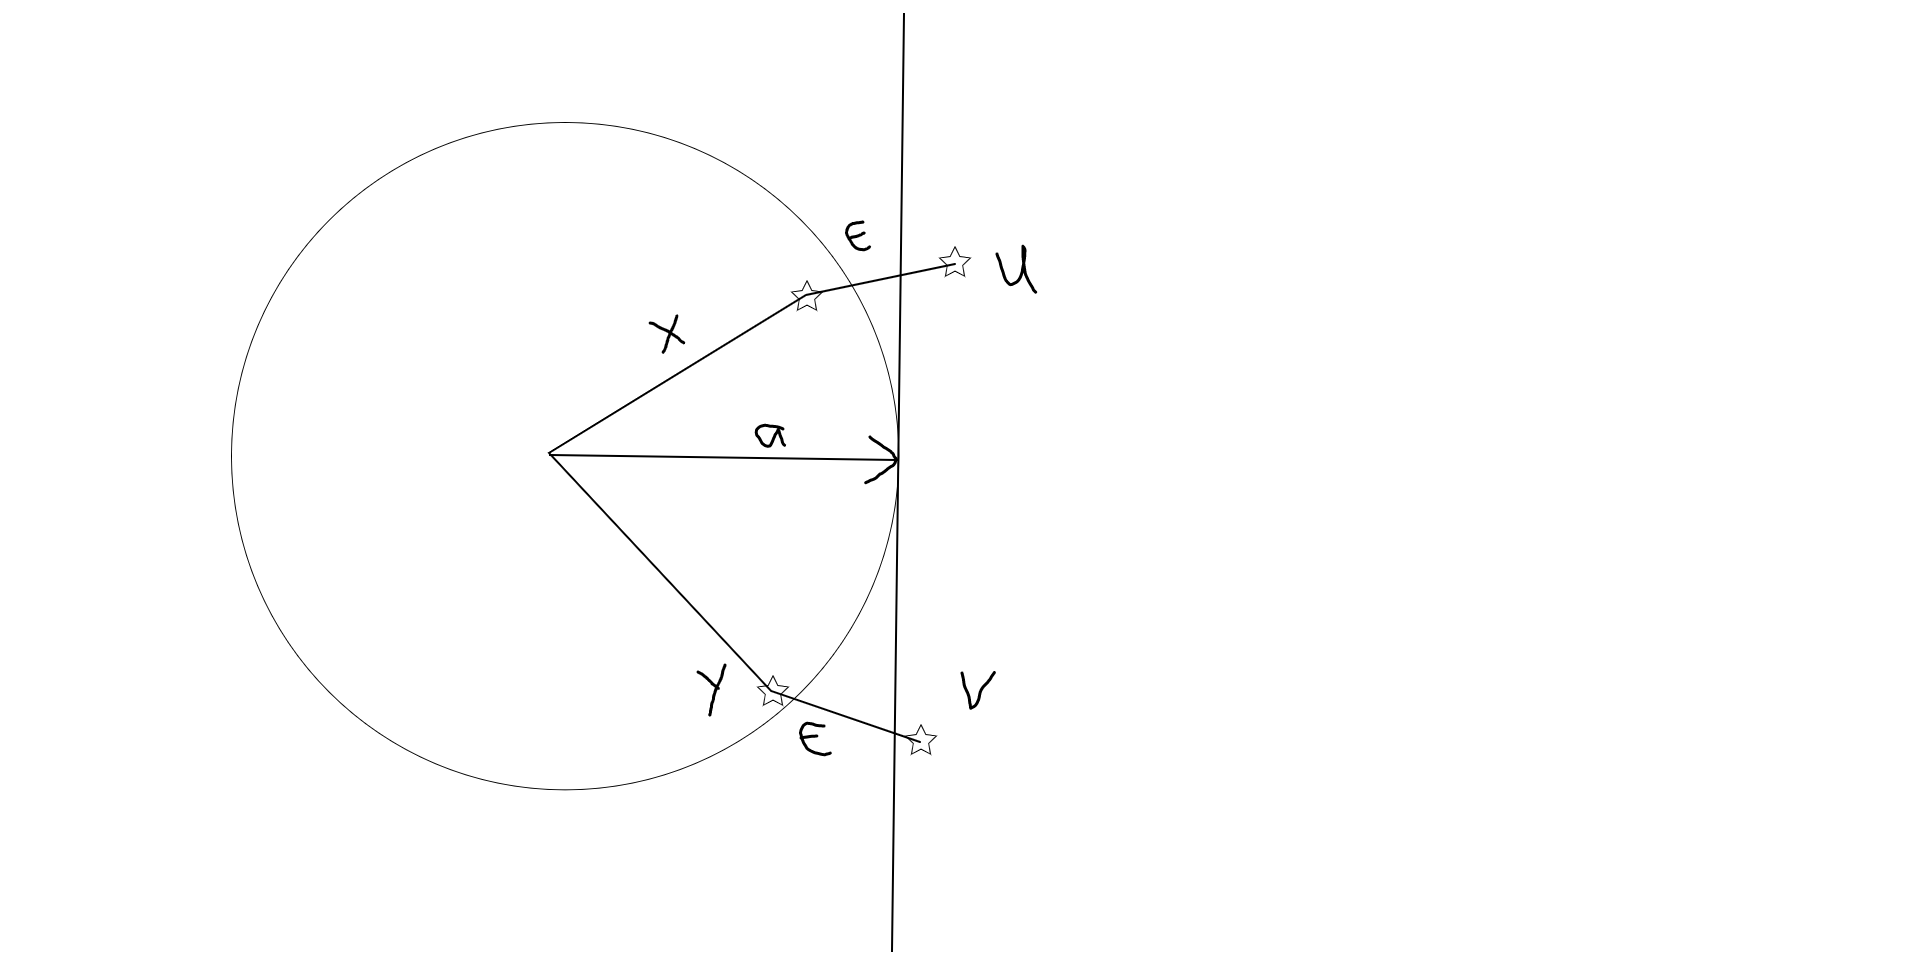
\includegraphics[width=300px]{images/first_lemma.png}
	\caption{
		The distances from $u$, $v$ to $x$, $y$ are less than $\epsilon$ respectively, and $x$ and $y$ lie within a sphere of radius $\|a\|$.
		Also, $a^Tx \le a^Ta$ separates the sphere from $u$ and $v$.
	}
	\label{first_lemma}
\end{figure}
The following lemma is illustrated in \cref{first_lemma}.
\begin{lemma}
\label{properties_of_a_circle}
Suppose that $x, y, u, v, a \in \Rn$ and $0 < \epsilon \le 1$ are given satisfying
\begin{align*}
\|x\| \le \|a\|, \quad
\|y \| \le \|a\|, \quad
\|x - u \| \le \epsilon, \quad
\|y - v \| \le \epsilon, \quad
a^T u \ge a^T a, \quad
a^T v \ge a^T a.
\end{align*}
Then
\begin{align*}
\|x - y\| \le 8(1 + \|a\|) \sqrt{\epsilon}.
\end{align*}
\end{lemma}
\begin{proof}
If $\|a\| = 0$, then $x = y = 0$ so that $\|x - y\| = 0$.
We may now assume that $a \ne 0$.
We can combine
$
a^Tx  \le \|a\| \|x\| \le \|a\|^2 = a^T a
% a^Ty  \le \|a\| \|y\| \le \|a\|^2 = a^T a
$
with
$
a^Tx = a^T(x - u) + a^T u \ge a^Ta - \|a\| \epsilon
% a^Ty = a^T(y - v) + a^T v \ge a^Ta - \|a\| \epsilon
$
to see
$
a^Ta - \|a\|\epsilon \le a^Tx \le a^Ta \Longrightarrow 0 \le a^Ta - a^Tx \le \|a\| \epsilon.
% a^Ta - \|a\|\epsilon \le a^Ty \le a^Ta \Longleftrightarrow 0 \le a^Ta - a^Ty \le \|a\| \epsilon 
$
By symmetry, $0 \le a^Ta - a^Ty \le \|a\| \epsilon$ so that
\begin{align*}
\left| a^Tx - a^Ty \right| \le \|a\|\epsilon.
\end{align*}


% 
% \begin{align*}
% \left(a^Ta - a^Tx\right)^2 \le \|a\|^2 \epsilon
% \end{align*}
% 
% \begin{align*}
% \end{align*}

Considering this identity further, we see
$
a^Ta - \|a\| \epsilon \le a^Tx \le \|a\|\|x\| 
\Longrightarrow \|a\| - \epsilon \le  \frac{a}{\|a\|}^T x \le \|x\| 
\Longrightarrow -\|a\| + \epsilon \ge  -\frac{a}{\|a\|}^T x \ge -\|x\| 
\Longrightarrow 0 \le \|x\| -\frac{a}{\|a\|}^T x \le \|x\|-\|a\| + \epsilon \le \epsilon
$
and
$
|\|x\| + \frac{a}{\|a\|}^T x| \le \|x - \frac{a}{\|a\|}^T x\| + 2|\frac{a}{\|a\|}^T x| \le \epsilon + 2\|x\| \le 2\|a\| + \epsilon
$.
We multiply these to find
\begin{align*}
\sqrt{\|x\|^2 - \frac{\left(a^Tx\right)^2}{a^Ta}}
= \sqrt{\left(\|x\| - \frac{a}{\|a\|}^Tx\right)\left(\|x\| + \frac{a}{\|a\|}^Tx\right)}
\le \sqrt{2\|a\|\epsilon + \epsilon^2} \le \epsilon + \sqrt{2\|a\|\epsilon}.
\end{align*}



% Also, we see
% $
% 0 \le \left\|a - x\right\|^2 
% = \|a\|^2 + \|x\|^2 - 2a^Tx 
% \le \|a\|^2 + \|x\|^2 - 2\left(a^Ta - \|a\|\epsilon\right)
% = \|x\|^2 - \|a\|^2 + 2\|a\|\epsilon
% $
% so that
% $
% \|a\|^2 - 2\|a\|\epsilon \le \|x\|^2 \le \|a\|^2
% \Longrightarrow 0 \le \|a\|^2 - \|x\|^2 \le 2\|a\|\epsilon.
% $
% By symmetry,
% $
% 0 \le \|a\|^2 - \|y\|^2 \le 2\|a\|\epsilon
% $
% and we see
% \begin{align*}
% \left|\|x\|^2 - \|y\|^2\right| \le 2 \|a\|\epsilon.
% \end{align*}

Because
$
\left(x - \frac{a^Tx}{a^Ta} a\right)^T \frac{a^Tx}{a^Ta} a = \frac{a^Tx}{a^Ta} a^Tx - \left(\frac{a^Tx}{a^Ta}\right)^2a^Ta = 0,
$
% \left(y - \frac{a^Ty}{a^Ta} a\right)^T \frac{a^Ty}{a^Ta} a = \frac{a^Ty}{a^Ta} a^Ty - \left(\frac{a^Ty}{a^Ta}\right)^2a^Ta = 0 \\
we can compute
$
\|x\|^2 = \left\|x - \frac{a^Tx}{a^Ta} a + \frac{a^Tx}{a^Ta} a\right\|^2 = \left\|x - \frac{a^Tx}{a^Ta} a \right\|^2 +\frac{\left|a^Tx\right|^2}{a^Ta}
$
% \|y\|^2 = \left\|y - \frac{a^Ty}{a^Ta} a + \frac{a^Ty}{a^Ta} a\right\|^2 = \left\|y - \frac{a^Ty}{a^Ta} a \right\|^2 +\left|a^Ty\right|^2
so that 
$
\left\|x - \frac{a^Tx}{a^Ta} a \right\| = \sqrt{\|x\|^2 - \frac{\left|a^Tx\right|^2}{a^Ta}}.
$
%  \left\|y - \frac{a^Ty}{a^Ta} a \right\| = \sqrt{\|y\|^2 - \left|a^Ty\right|^2}
By symmetry,
$
\left\|y - \frac{a^Ty}{a^Ta} a \right\| = \sqrt{\|y\|^2 - \frac{\left|a^Ty\right|^2}{a^Ta}},
$
so that

\begin{align*}
\left\|x - \frac{a^Tx}{a^Ta} a - y + \frac{a^Ty}{a^Ta} a \right\|
\le \left\|x - \frac{a^Tx}{a^Ta} a \right\| + \left\|y - \frac{a^Ty}{a^Ta} a \right\|
\le 2\epsilon + 2\sqrt{2\|a\|\epsilon}.
\end{align*}

% \begin{align*}
% \left\|x - \frac{a^Tx}{a^Ta} a \right\|^2 - \left\|y - \frac{a^Ty}{a^Ta} a \right\|^2
% = \|x\|^2 - \|y\|^2 + \left(-\left|a^Tx\right|^2 + \left|a^Ty\right|^2\right) \\
% \left|\left\|x - \frac{a^Tx}{a^Ta} a \right\|^2 - \left\|y - \frac{a^Ty}{a^Ta} a \right\|^2\right|
% \le \left|\|x\|^2 - \|y\|^2\right| + \left|\left|a^Tx\right|^2 - \left|a^Ty\right|^2\right| \\
% \le 2 \|a\|\epsilon + 2 |a^Tx| \|a\|\epsilon + \|a\|^2\epsilon^2 \\
% \Longrightarrow 
% \left|\left\|x - \frac{a^Tx}{a^Ta} a \right\| - \left\|y - \frac{a^Ty}{a^Ta} a \right\|\right|
% \le \sqrt{2 \|a\|\epsilon + 2 |a^Tx| \|a\|\epsilon + \|a\|^2\epsilon^2}
% \le \|a\|\epsilon + \sqrt{2 \|a\|\epsilon\left(1 + |a^Tx|\right)}
% \end{align*}


% \begin{align*}
% \left\|x - \frac{a^Tx}{a^Ta} a - \left(y - \frac{a^Ty}{a^Ta} a\right)\right\|^2
% = \left\|x - \frac{a^Tx}{a^Ta} a\right\|^2 + \left\|y - \frac{a^Ty}{a^Ta} a\right\|^2 - 2\left(x - \frac{a^Tx}{a^Ta} a\right)^T\left(y - \frac{a^Ty}{a^Ta} a\right) \\
% = \left\|x - \frac{a^Tx}{a^Ta} a\right\|^2 + \left\|y - \frac{a^Ty}{a^Ta} a\right\|^2 - 2\left(x^Ty - \frac{a^Tya^Tx}{a^Ta}\right) \\
% \end{align*}
% 
% \begin{align*}
% \left\|x - \frac{a^Tx}{a^Ta} a - \left(y - \frac{a^Ty}{a^Ta} a\right)\right\|^2
% = \left\|x - \frac{a^Tx}{a^Ta} a\right\|^2 + \left\|y - \frac{a^Ty}{a^Ta} a\right\|^2 - 2\left(x - \frac{a^Tx}{a^Ta} a\right)^T\left(y - \frac{a^Ty}{a^Ta} a\right) \\
% = \left\|x - \frac{a^Tx}{a^Ta} a\right\|^2 + \left\|y - \frac{a^Ty}{a^Ta} a\right\|^2 - 2\left(x^Ty - \frac{a^Tya^Tx}{a^Ta}\right) \\
% \end{align*}



Finally, we combine everything to see
\begin{align*}
\|x - y\| 
\le \left\|x - \frac{a^Tx}{a^Ta} a - \left(y - \frac{a^Ty}{a^Ta} a\right)\right\| + |a^Tx - a^Ty|
\le (2 + \|a\|)\epsilon + 2\sqrt{2\|a\|\epsilon} \\
\le \left(2 + 2\sqrt{2\|a\|} + \|a\|\right)\sqrt{\epsilon}
\le \left(\sqrt{2} + \sqrt{\|a\|}\right)^2 \sqrt{\epsilon}
\le \left(2\max\{\sqrt{2},\sqrt{\|a\|}\}\right)^2 \sqrt{\epsilon} \\
\le 4\max\{2,\|a\|\} \sqrt{\epsilon}
\le 8\max\{1,\|a\|\} \sqrt{\epsilon}
\le 8(1 + \|a\|) \sqrt{\epsilon}
\end{align*}
% is small.
% = \epsilon \|a\| \left(2 + 2|a^Tx| + \|a\|\epsilon\right) \\

% \begin{align*}
% \left\|x - \frac{a^Tx}{a^Ta} a \right\| - \left\|y - \frac{a^Ty}{a^Ta} a \right\|
% = \sqrt{\|x\|^2 - \|y\|^2} - \sqrt{\left|a^Tx\right|^2 + \left|a^Ty\right|^2}
% \end{align*}

% \begin{align*}
% |x - y| \le \epsilon \\
% \Longleftrightarrow x - \epsilon \le y \le x + \epsilon \\
% \Longleftrightarrow x^2 - 2x\epsilon - \epsilon^2 \le x^2 - 2x\epsilon + \epsilon^2 \le y^2 \le x^2 + 2x\epsilon + \epsilon^2 \\
% \Longleftrightarrow  |x^2 - y^2| \le 2 x \epsilon + \epsilon^2
% \end{align*}
% 
% \begin{align*}
% \epsilon \le x^2 \\
% \Longrightarrow \sqrt{\epsilon} \le x \\
% \Longrightarrow 2\epsilon \le 2x\sqrt{\epsilon} \\
% \Longrightarrow x^2 - 2x\sqrt{\epsilon} + \epsilon \le x^2 - \epsilon \\
% \Longrightarrow x - \sqrt{\epsilon} \le \sqrt{x^2 - \epsilon}
% \end{align*}
% 
% \begin{align*}
% \left|x^2 - y^2\right| \le \epsilon \\
% \Longleftrightarrow x^2 - \epsilon \le y^2 \le x^2 + \epsilon \\
% \Longleftrightarrow x - \sqrt{\epsilon} \le \sqrt{x^2 - \epsilon} \le y \le \sqrt{x^2 + \epsilon} \le x + \sqrt{\epsilon} \\
% \Longleftrightarrow |x - y| \le \sqrt{\epsilon}
% \end{align*}

% \begin{align*}
% x^Tx \ge \frac{\|x\|}{\|a\|} a^T x
% \ge \frac{\|x\|}{\|a\|}\left(a^Ta - \|a\|\epsilon\right)
% \ge \|x\|\|a\| - \|x\| \epsilon 
% \ge \|x\|\left(\|a\| - \epsilon\right)
% \end{align*}
% 
% \begin{align*}
% x = x - \frac{a^Tx}{a^Ta} a + \frac{a^Tx}{a^Ta} a \\
% y = y - \frac{a^Ty}{a^Ta} a + \frac{a^Ty}{a^Ta} a
% \end{align*}
% 
% \begin{align*}
% \|x - y\| =
% \left\| x - \frac{a^Tx}{a^Ta} a  \right\|
% \end{align*}

\end{proof}



For any two convex sets $S_1$ and $S_2$, define
\begin{align}
\convexdistance\left(S_1, S_2\right) = \max_{s' \in S_1 \cup S_2} \min_{s \in S_1 \cap S_2} \|s' - s\|. \label{define_a_difference_between_sets}
\end{align}

\begin{lemma}
\label{board_tied_to_sphere}
Let $\convexdistance$ be defined by \cref{define_a_difference_between_sets}.
Let $g \in \Rn$ and let $S, S' \subseteq \Rn$ be convex and non-empty.
Suppose that $0 < \epsilon \le 1$ is given with $D\left(S, S'\right) \le \epsilon$.
Then 
\begin{align*}
\|P_{S}(g) - P_{S'}(g)\| \le 8\left(1 + \|P_{S \cap S'}(g) - g\|\right) \sqrt{\epsilon}.
\end{align*}
\end{lemma}
\begin{proof}
Because $\convexdistance(S, S') \le \epsilon$, we know that $S \cap S' \ne \emptyset$.
Let $x = P_S(g) - g$ and $y = P_{S'}(g) - g$, $u = P_{S \cap S'}(g + x) - g$, $v = P_{S \cap S'}(g + y) - g$, $a = P_{S \cap S'}(g) - g$.
Then, because $S \cap S' \subseteq S$ and $S \cap S' \subseteq S'$ we have
$\|x\| = \|P_S(g) - g\| \le \|P_{S \cap S'} (g) - g\| = \|a\|$ and $\|y\| \le \|a\|$.
Also, by optimality conditions of $a$, we know that the plane $a^Tx \ge a^Ta$ separates $S \cap S'$ from $g$.
In particular, $a^Tu \ge a^Ta$ and $a^Tv \ge a^Ta$.
Finally, because $\convexdistance(S, S') \le \epsilon$, we have $\|x - u\| = \|P_{S \cap S'}\left(P_S(g)\right)\| \le \epsilon$ and $\|y - v\| \le \epsilon$.
Thus, \cref{properties_of_a_circle} informs us
$\|P_S(g) - P_{S'}(g)\| = \|x - y\| \le 8(1 + \|a\|) \sqrt{\epsilon}$.
\end{proof}


\begin{corollary}
Let $\convexdistance$ be defined by \cref{define_a_difference_between_sets}.
Let $g, g' \in \Rn$ and let $S, S' \subseteq \Rn$ be convex and non-empty.
Suppose that $0 < \epsilon \le 1$ is given with $D\left(S, S'\right) \le \epsilon$ and $\|g - g'\| \le \epsilon$.
Then $\|P_S(g) - P_{S'}(g')\| \le 9\left(1 + \|P_{S \cap S'}(g) - g\|\right) \sqrt{\epsilon}$.
\end{corollary}
\begin{proof}
Notice
\begin{align*}
\|P_S(g) - P_{S'}(g')\| 
\le \|P_S(g) - P_{S'}(g)\| + \|P_{S'}(g) - P_{S'}(g')\| 
\le \|P_S(g) - P_{S'}(g)\| + \|g - g'\| \\
\le 8\left(1 + \|P_{S \cap S'}(g) - g\|\right) \sqrt{\epsilon} + \epsilon
\le 9\left(1 + \|P_{S \cap S'}(g) - g\|\right) \sqrt{\epsilon}.
\end{align*}
\end{proof}

\begin{lemma}
\label{the_lemma_to_end_all_lemmas}
Let $\convexdistance$ be defined by \cref{define_a_difference_between_sets}.

Let
$A, A' \in \mathbb \mathbb R^{m \times n}$;
$b, b' \in \mathbb \mathbb R^{m}_{\ge 0}$;
$C, C' \in \mathbb \mathbb R^{m' \times n}$;
$d, d' \in \mathbb \mathbb R^{m'}_{\ge 0}$;
unit vector $u \in \Rn$;
$\delta_l, \delta_u, \delta_{\alpha}, \delta_r > 0$;
be given such that 
\begin{align*}
\begin{array}{cccc}
\delta_r \|A_i\| \le b_i,			&
Cu \ge \delta_{\alpha} e,			&
\delta_l \le \|A_i\| \le \delta_u	\\
\delta_r \|A_i'\| \le b_i',			&
C'u \ge \delta_{\alpha} e, 			&
\delta_l \le \|A'_i\| \le \delta_u.
\end{array}
\end{align*}
For any $p \in \Rn$ and $r > 0$ define the sets
\begin{align*}
\begin{array}{ccccc}
S  &= \bigg\{x \in \Rn \bigg|& A (x - p) \le b ,& C (x - p) \le d ,& \|x - p\| \le r \bigg\}, \\
S' &= \bigg\{x \in \Rn \bigg|& A'(x - p) \le b',& C'(x - p) \le d',& \|x - p\| \le r \bigg\}.
\end{array}
\end{align*}
For any $0 < \epsilon < r$ there exists $\delta > 0$ such that if
\begin{align*}
\begin{array}{cccc}
\|A - A'\|_{\infty} \le \delta,	& \|b - b'\|_{\infty} \le \delta,		& \|C - C'\|_{\infty} \le \delta,	& \|d - d'\|_{\infty} \le \delta
\end{array}
\end{align*}
then
\begin{align*}
D(S, S') \le \epsilon.
\end{align*}



% \delta_1 \le \delta_2 \|A_i\| \le b_i, 
% \delta_1 \le \delta_2 \|A'_i\| \le b'_i, \\
% \gamma = \frac{2}{\delta_1}\left(1 + \|y\|\right), 
% \epsilon \le \min\left\{\gamma^{-1}\right\}.


\end{lemma}
% y - z  =       A        ^T\mu  + C^T\lambda  \\
% y - z' = \left(A'\right)^T\mu' + C^T\lambda' \\
% t &=  \max_{\substack{i \in [m] \\ A'_i(z - p) > b'_i}} \frac{A'_i (z - p) - b'_i}{A'_i (z - p)} \\

\begin{proof}
% (1 + r)\left[1 + \delta_{\alpha}^{-1} \left(\delta_2 + 1\right)\right]
Let $x \in S$, and define
\begin{align*}
\begin{array}{cccccc}
\lambda &=& \delta_{\alpha}^{-1}(r + 1) (\delta_u + 2), &
\gamma &=& 2\lambda(\delta_r \delta_u)^{-1}, \\
\eta    &=& \frac 1 2 \epsilon\delta_{\alpha}(r+2)^{-1}(r + 1)^{-1}, &
\delta &=& \min\bigg\{
1,
\gamma^{-1},
\frac 1 2 {\epsilon} (\gamma r)^{-1},
\eta
\bigg\}, \\
s &=& \delta(r + 1)\delta_{\alpha}^{-1}, &
z &=& x - su, \\
t &=& \max\left\{\gamma \delta, s(r+s)^{-1}\right\}, &
v &=& (1-t)z + t p.
\end{array}
\end{align*}
The construction of $v$ has the following intuition:
to travel to $v$ from $x$, we
\begin{itemize}
\item first travel a distance $s$ along $-u$ to reach $z$ (where we will show $C'(z-p) \le d'$),
\item then travel a fraction $t$ of the distance back to $p$ (where both $A'(v - p) \le b'$ and $\|v-p\| \le r$).
\end{itemize}
Throughout the remainder of this proof, we will show $v \in S'$ and $\|x - v\| \le \epsilon$.
The result then follows from the symmetry of $S$ and $S'$.


For each $i \in [m]$,
\begin{align*}
0 \le C_i'(x-p) - d_i'
\le C_i(x - p) - d_i + (C_i' - C_i)(x-p) + d_i - d_i'  \\
\le 0 + \|C_i' - C_i\| \|x - p\| + \|d_i - d_i'\| 
\le \delta (r+1)
= \delta_{\alpha} s \le sC_i'u
\end{align*}
so that
\begin{align}
-sC_i'u \le d_i' - C_i'(x - p) \Longrightarrow C'(z - p) = C'(x - su - p) \le d'. \label{reun_eqn3}
\end{align}

\begin{comment}
Explanation for next sentence:
\begin{align*}
s\delta_u + \delta \left(s + r\right) + \delta 
&= \frac{\delta(r + 1)}{\delta_{\alpha}}\delta_u + \delta \left(s + r\right) + \delta \\
&\le \delta \left[(r + 1)\frac{\delta_u}{\delta_{\alpha}} + (r+1)\frac{\delta}{\delta_{\alpha}} + r + 1\right] \\
&\le \delta (r + 1) \left[\frac{\delta_u}{\delta_{\alpha}} + \frac{\delta}{\delta_{\alpha}} + 1\right] \\
&\le \delta (r + 1) \left[\frac{\delta_u}{\delta_{\alpha}} + \frac{1}{\delta_{\alpha}} + \frac{1}{\delta_{\alpha}}\right] \\
&\le \delta \delta_{\alpha}^{-1}(r + 1) (\delta_u + 2)
\end{align*}
\end{comment}
Also, without loss of generality, $\delta_{\alpha} \le 1$, so that
\begin{align}
A_i'(z - p) - b_i' 
&= - s A_iu + A_i(x - p) - b_i + (A_i' - A_i)(z - x + x - p) + (b_i' - b_i) \nonumber \\
&\le s \|A_i\|\|u\| + 0 + \|A_i' - A_i\|\left[\|z - x\| + \|x - p\|\right] + \|b_i'-b_i\| \nonumber \\
&\le s\delta_u + \delta \left(s + r\right) + \delta \le \lambda \delta \label{reun_eqn1}
\end{align}
so that whenever $A_i'(z - p) > b_i'$,
\begin{align}
\left|A_i'(z - p)\right| 
\ge |b_i'| - \left| A_i'(z - p) - b_i'\right| 
\ge \delta_r\|A_i'\| - \lambda \delta 
\ge \delta_r \delta_u - \lambda \delta \ge \frac 1 2 \delta_r \delta_u. \label{reun_eqn2}
\end{align}
% \Longrightarrow \frac 1 {\left|A_i'(z - p)\right|} \le \frac 2 {\delta_1 \delta_3}. 

% &= A_i(z - p) - b_i + (A_i' - A_i)(z - p) + (b_i' - b_i) \\
% \begin{align*}
% A_i(z - p) - b_i = A_i(x - p) - b_i - s A_iu \le 0 + s \|A_i\| \|u\| \le s\delta_2
% \end{align*}
% so that

% \begin{align*}
% \lambda \delta \le \frac 1 2 \delta_1 \delta_3
% \end{align*}
% \begin{align*}
% (1 - t) A_i'\left[z - p\right] \le b_i' \\
% A_i'\left[(1-t) z + tp - p\right] \le b_i'
% \end{align*}

Dividing \cref{reun_eqn1} by \cref{reun_eqn2}, we find
\begin{align*}
\frac{A'_i (z - p) - b'_i}{A'_i (z - p)} \le \frac{2\lambda}{\delta_r \delta_u}\delta = \gamma \delta \le 1
\end{align*}
which means $t = \max\left\{\gamma \delta, \frac{s}{r+s}\right\} \in [0, 1]$.
Also, note that for each $i \in [m]$, if $A_i'(z - p) > b_i'$, then
\begin{align*}
t \ge \frac{A'_i (z - p) - b'_i}{A'_i (z - p)}
\Longrightarrow (1-t) A'_i (z - p) \le b'_i.
\end{align*}
But if $A_i'(z - p) \le b_i'$, then $t \le 1$ and $b_i' \ge 0$ provide the same identity.
Therefore, 
\begin{align*}
A'(v - p) = A' \bigg[(1-t) z + tp - p\bigg] = (1-t) A' (z - p) \le b'.
\end{align*}
Because $t \in [0, 1]$, \cref{reun_eqn3} and convexity imply $C'(v - p) \le d$.
Lastly, $t \ge \frac{s}{r + s} \Longrightarrow (1 - t) \left(r + s\right) \le r$, so that
\begin{align*}
\|v - p\| = \|(1-t)z + t p - p\| = (1 - t) \|z - p\| \le (1 - t) \left(\|x - p\| + s\right) \le (1 - t) \left(r + s\right) \le r
\end{align*}
and $v \in S'$.
\begin{comment}
Explanation:
\begin{align*}
t \ge \frac{s}{r + s} \\
 tr + ts \ge s \\
- tr - ts \le -s \\
r - tr + s - ts \le r \\
(1 - t) r + (1 - t)s \le r \\
(1 - t) \left(r + s\right) \le r \\
\end{align*}
\end{comment}

Finally, we will show $\|v - x\| \le \epsilon$.
Notice that $\delta \le \eta = \frac{\epsilon\delta_{\alpha}}{2(r+2)(r + 1)} \Longrightarrow s \le \frac{\epsilon}{4 + 2r - \epsilon}$, which implies two things.
First, it means $s \le \frac{\epsilon}{2r - \epsilon}$ so that
$\frac {s}{1 + s} \le \frac {\epsilon} {2r}. $
Combine this with $\delta \le \frac {\epsilon} {2\gamma r}$ to find that $tr \le \frac 1 2 \epsilon$.
Secondly, it means that
$s \le \frac{\epsilon}{4}$ so that $(1 + t)s \le \frac 1 2 \epsilon$.
Combining these produces,
\begin{align*}
\|x - v\| 
\le \|x - z\| - \|z - v\| 
= s + t \|p - z\| 
\le s + t \left(r + s\right) 
= (1 + t)s + tr
\le \frac 1 2 \epsilon + \frac 1 2 \epsilon = \epsilon.
\end{align*}
% = s + \|(1-t) z + tp - z\| 

\begin{comment}
Explanations:
\begin{align*}
\delta \le \frac{\epsilon\delta_{\alpha}}{2(r+2)(r + 1)}
\le \frac{\epsilon\delta_{\alpha}}{(4 + 2r - \epsilon)(r + 1)} 
\Longrightarrow \frac{\delta(r + 1)}{\delta_{\alpha}}  \le \frac{\epsilon}{4 + 2r - \epsilon} \Longrightarrow
s\le \frac{\epsilon}{4 + 2r - \epsilon}
\end{align*}
\begin{align*}
s\le \frac{\epsilon}{(2r - \epsilon)} \Longrightarrow
s(2r - \epsilon)\le \epsilon \Longrightarrow
2rs \le \epsilon(1 + s) \Longrightarrow
\frac {s}{1 + s} \le \frac {\epsilon} {2r}
\end{align*}
\begin{align*}
s \le \frac{\epsilon}{4 + 2r - \epsilon} \le \frac 1 4 \epsilon \Longrightarrow
(1 + t)s \le 2s \le \frac 1 2 \epsilon
\end{align*}
\end{comment}
\end{proof}

\subsubsection{Simplifed Results}
\label{simplifed_bounded_projection}


\begin{definition}
\label{criteria_from_contradiction}
A sequence $S \subseteq\naturals \times \naturals$ satisfies this definition if
% is called a \emph{Cauchy pair-subsequence} if
% Let $l, k \in S \subseteq \naturals$, where $S$ is such that the subsequence $\{\xk\}_{k \in S}$ is Cauchy.
for any $\epsilon > 0$, there exists $k_0 \in \naturals$ such that if $(k, l) \in S$ with $k, l \ge k_0$, 
then 
$\left\|\xk - \xl \right\| \le \epsilon$.
% There exists $x^{\star}$ such that $\lim_{k\to\infty} \xk = x^{\star}$.
\end{definition}


\begin{lemma}
\label{model_gradients_are_cauchy}
Suppose that the assumptions for
\cref{lipschitz_gradients_assumption}, \cref{huffman_constant_is_bounded}, \cref{accuracy_is_satisfied}
hold.

If $S$ satisfies \cref{criteria_from_contradiction}, then for each $i \in [m]$ and any $\epsilon > 0$, there is a $k_0 \in \naturals$
such that if $(k, l) \in S$ and $k, l \ge k_0$, then $\left\|\gmcik - \gmcil \right\| \le \epsilon$.
\end{lemma}
\begin{proof}
Let $\epsilon > 0$ be arbitrary.
By \cref{delta_to_zero}, we can choose $N_1$ such that $\lipgrad \left\|\xk - \xl \right\| \le \frac 1 3 \epsilon$.
Also, because every convergent sequence is Cauchy, we can choose an $N_2 \in \naturals$ such that $\kappa_g \dk^2 \le \frac 1 3 \epsilon $ whenever $k \ge N_2$.
Choose $N_0 = \max\{N_1, N_2\}$, and let $d, k \ge N_2$.
The triangle inequality states
\begin{align*}
\left\|\nabla \mcik\left(\xk\right) - \nabla \mcil\left(\xl\right) \right\|
\le 
\left\|\nabla \mcik\left(\xk\right) - \nabla c_i\left(\xk\right) \right\|
+ \left \| \nabla \mcil\left(\xl\right) - \nabla c_i\left(\xl\right) \right \| \\
+ \left\|\nabla c_i\left(\xk\right) - \nabla c_i\left(\xl\right)\right\|.
\end{align*}
Using \cref{accuracy_is_satisfied} and \cref{lipschitz_gradients_assumption}, we see
\begin{align*}
\left\|\nabla \mcik\left(\xk\right) - \nabla \mcil\left(\xl\right) \right\|
\le \kappa_g \left(\dk^2 + \dl^2\right) + \lipgrad \left\|\xk - \xl \right\|.
\end{align*}
By our choice of $N_0$, we see that
\begin{align*}
\left\|\nabla \mcik\left(\xk\right) - \nabla \mcil\left(\xl\right) \right\|
\le \frac 1 3 \epsilon + \frac 1 3 \epsilon + \frac 1 3 \epsilon = \epsilon.
\end{align*}
\end{proof}
% \left\|\mcik\left(\xk\right) - \mcik\left(\xl\right) \right\| + \left \| \mcik\left(\xl\right) - \mcil\left(\xl\right) \right\|





Let $\minangledelta$ be defined by \cref{minangleassumption_alt} and define
% such that if $\dk \le \minangledelta$ and
\begin{align}
\activeindicesk = \left\{i \in [m] \bigg| -c_i\left(\xk\right) \le \minangledelta \left\|\gmcik\right\| \right\}. \label{define_activeindicesk}
\end{align}


% \begin{align*}
% ? =  \\
% c_i\left(\xk\right) + \gmcik^T \gk
% \end{align*}

The following observation follows directly from the definition:
\begin{lemma}
\label{doesntreallyneedtobesaid}
Let $\activeindicesk$, $\zik$, $\minangledelta$ be defined by \cref{define_activeindicesk}, \cref{define_z}, and \cref{minangleassumption_alt} respectively.
If $i \in \activeindicesk$, then $\zik \in B_{\infty}\left(\xk, \minangledelta \right)$.
\end{lemma}
\begin{proof}
If $c_i\left(\xk\right) = 0$, then $\zik = \xk \in B_{\infty}\left(\xk, \minangledelta \right)$.
Otherwise, $\left\|\gmcik\right\| \ge \frac{-c_i\left(\xk\right)}{\minangledelta} \ge 0$, so
\begin{align*}
\zik = \xk - \frac{m^{(k)}_{c_i}\left(\xk\right)}{\left\|\gmcik\right\|^2} \gmcik 
\Longrightarrow \left\|\xk - \zik \right\|= -\frac{c_i\left(\xk\right)}{\left\|\gmcik\right\|} \le \minangledelta.
\end{align*}
\end{proof}


\begin{lemma}
\label{underbound}
Suppose that \cref{mingradassumption} holds.

Let $\activeindicesk$ be defined by \cref{define_activeindicesk}.
There exists $\activegradmin > 0$ and $k_0 \in \naturals$ such that if $k \ge k_0$, then
for all $i \in \activeindicesk$,
\begin{align*}
\left\|\gmcik\right\| \ge \activegradmin.
\end{align*}
\end{lemma}
\begin{proof}

Let $\mingradepsilon$ and $\mingrad$ be defined by \cref{mingradassumption}.
Define
\begin{align}
\label{define_activegradmin}
\activegradmin = \min\left\{\mingrad, \frac{\mingradepsilon}{\sqrt{n} \minangledelta}\right\}.
\end{align}

By \cref{mingradassumption}, if $-c_i\left(\xk\right) \le \mingradepsilon$, then $\nabla c_i\left(\xk\right) \ge \mingrad \ge \activegradmin$.
We may now assume that $-c_i\left(\xk\right) \ge \mingradepsilon$.
Because $i \in \activeindicesk$, using \cref{define_z}, we have
\begin{align*}
\sqrt{n} \minangledelta \ge \left\|\xk - \zik \right\|
= \frac{-c_i\left(\xk\right)}{\left\|\gmcik\right\|}
\ge \frac{\mingradepsilon}{\left\|\gmcik\right\|}
\Longrightarrow
\left\|\gmcik\right\| \ge \frac{\mingradepsilon}{\sqrt{n} \minangledelta} \ge \activegradmin
\end{align*}
\end{proof}



\begin{lemma}
\label{yet_another_bound_on_a_u}
Suppose that the assumptions for \cref{underbound}, \cref{accuracy_is_satisfied} hold.
Suppose that the assumptions for \cref{model_gradients_are_cauchy} hold.

Let $\activeindicesk$ be defined by \cref{define_activeindicesk}.
There exists $k_0 \in \naturals$, scalar $\minactivealpha > 0$, and unit vector $\activedirk \in \Rn$ such that if 
$k \ge k_0$, then $\forall i \in \activeindicesk$
\begin{align*}
\gmcik^T \activedirk \ge \minactivealpha
\quad \textrm{and} \quad
\nabla c_i\left(\xk\right)^T \activedirk \ge \minactivealpha.
\end{align*}

Furthermore, if a set $S$ satisfies \cref{criteria_from_contradiction}, and $(k, l) \in S$, $l \ge k_0$, then $\forall i \in \activeindicesk$
\begin{align*}
\gmcil^T \activedirk \ge \minactivealpha.
\end{align*}
\end{lemma}
\begin{proof}

Let 
$\minanglealpha$ and $\minangledelta$ be defined by \cref{minangleassumption_alt};
$\kappa_g$ be defined by \cref{accuracy_is_satisfied}; 
and $\activegradmin$ be defined by \cref{define_activegradmin}.

Define 
\begin{align}
\minactivealpha = \frac 1 2 \minanglealpha \activegradmin. \label{define_minactivealpha}
\end{align}

By \cref{delta_to_zero}, we know there exists $k_1 \in \naturals$ such that if $k \ge k_1$, then
\begin{align*}
\dk \le \minangledelta \quad \textrm{and} \quad  \dk \le \sqrt{\frac {\minanglealpha \activegradmin} {2 \kappa_g}}.
\end{align*}
Thus, by \cref{doesntreallyneedtobesaid}, \cref{minangleassumption_alt}, and \cref{underbound} we know 
there exists a unit vector $\minangledirk\in\Rn$ and $k_2 \in \naturals$ such that 
for all $i \in \mathbb I^{(k)}$, $k \ge k_2$:
\begin{align*}
-\frac {\gmcik}{\left\|\gmcik\right\|} ^T\minangledirk \ge \minanglealpha \Longrightarrow \gmcik^T\left(-\minangledirk\right) \ge \minanglealpha \activegradmin
\end{align*}
Also, by \cref{accuracy_is_satisfied}, we have
\begin{align*}
\left\|\gmcik - \nabla c_i\left(\xk\right) \right\| \le \kappa_g \dk^2 \le \frac 1 2 \minanglealpha \activegradmin
\end{align*}
so that
\begin{align*}
\nabla c_i\left(\xk\right)^T \left(-\minangledirk\right) = 
\gmcik^T\left(-\minangledirk\right) + \left(\gmcik - \nabla c_i\left(\xk\right) \right)^T\left(-\minangledirk\right) \\
\ge \minanglealpha \activegradmin - \left\|\gmcik - \nabla c_i\left(\xk\right) \right\|\left\|\minangledirk\right\|
\ge \minanglealpha \activegradmin - \frac 1 2 \minanglealpha \activegradmin = \minactivealpha.
\end{align*}

Furthermore, if $(k, l) \in S$, then by \cref{model_gradients_are_cauchy} there exists $k_3 \in \naturals$ such that if $(k, l) \in S$ and $k, l \ge k_3$
\begin{align*}
\left\|\gmcik - \gmcil\right\| \le \frac {\minanglealpha \activegradmin} {2}
\end{align*}
and once again,
\begin{align*}
\gmcil \left(-\minangledirk\right) = 
\gmcik^T\left(-\minangledirk\right) + \left(\gmcik - \gmcil \right)^T\left(-\minangledirk\right)
\ge \minactivealpha.
\end{align*}
\end{proof}




% 
% 
% 
% \begin{align*}
% \left\|z - p\right\| = r \\
% r \le \left\|z' - p\right\| = r + \epsilon \\
% (z - p)^T (z' - p) \ge \|z - p\|^2
% \end{align*}
% 
% \begin{align*}
% \left\|z - z'\right\|
% \end{align*}
% 
% 
% 


% \begin{lemma}
% aabbcc
% \end{lemma}
% \begin{proof}
% By the mean value theorem, there exists $t \in [0, 1]$ such that
% \begin{align*}
% \end{align*}
% \end{proof}

Define
\begin{align}
\truefeasiblek &= \left\{ x \in \Rn \bigg| c_i\left(\xk\right) + \nabla c_i\left(\xk\right)^T \left(x - \xk\right) \le 0 \; \forall i \in [m] \right\} \label{define_truefeasiblek}
\end{align}


Let $\feasiblek$, $\truefeasiblek$ be defined by \cref{define_feasiblek} and \cref{define_truefeasiblek} respectively, for any fixed $k$, define
\begin{align}
\Amk &= \left\{ i \in [m] \bigg | c_i\left(\xk\right) + \gmcik^T\left( P_{\feasiblek}\left(\xk - \gk\right) - \xk\right) = 0\right\}, \label{tbbt_a1} \\
\Alk &= \left\{ i \in [m] \bigg | c_i\left(\xl\right) + \gmcil^T\left( P_{\feasiblel}\left(\xk - \gk\right) - \xl\right) = 0\right\}, \label{tbbt_a2} \\
\Ack &= \left\{ i \in [m] \bigg | c_i\left(\xk\right) + \nabla c\left(\xk\right)^T\left( P_{\truefeasiblek}\left(\xk - \gk\right) - \xk\right) = 0\right\}. \label{tbbt_a3}
\end{align}

\begin{lemma}
\label{norm_of_active_constraints_bounded_below}
Suppose that $\Amk$, $\Alk$, $\Ack$
are defined by
\cref{tbbt_a1}, \cref{tbbt_a2}, and \cref{tbbt_a3}.

Suppose that
\cref{mingradassumption}
and the assumptions for
\cref{accuracy_is_satisfied}, \cref{i_thought_i_proved_this_already}, and \cref{delta_to_zero}
are satisfied.
Suppose that a set $S$ satisfies \cref{criteria_from_contradiction}.
There exists $\deltalb > 0$ and $k_0 \in \naturals$ such that,
\begin{itemize}
\item if $k \ge k_0$ and $i \in \Amk \cup \Ack$,
\begin{align*}
\left\|\gmcik\right\| \ge \deltalb \quad \textrm{and} \quad
\left\|\nabla c_i\left(\xk\right) \right\| \ge \deltalb.
\end{align*}
\item if $k, l \ge k_0$, $(k, l) \in S$, and $i \in \Amk \cup \Alk$,
\begin{align*}
\left\|\gmcil\right\| \ge \deltalb.
\end{align*}
\end{itemize}
\end{lemma}
\begin{proof}

Let $\mingradepsilon > 0$ and $\mingrad > 0$ be defined by \cref{mingradassumption}
and $\maxmodelgrad \ge 1$ be defined by \cref{i_thought_i_proved_this_already}.
% and $\maxgrad$ be defined by \cref{bounded_gradients_lemma}.
Define
\begin{align*}
\deltalb = \min\left\{\frac 1 3 \mingrad, \frac 1 {6} \frac{\mingradepsilon}{\maxmodelgrad} \right\}.
\end{align*}

Before going through several cases, we make four observations.
First, \cref{i_thought_i_proved_this_already} and \cref{delta_to_zero} imply the existence of $k_1 \in \naturals$
such that if $k \ge k_1$, then
\begin{align*}
\left\|P_{\feasiblek}\left(\xk - \gk\right) - \xk\right\| 
\le \left\|\xk - \gk - \xk \right\| \le \maxmodelgrad.
\end{align*}
Secondly, \cref{accuracy_is_satisfied} and \cref{delta_to_zero} imply the existence of $k_2 \in \naturals$ such that if $k \ge k_2$, then
\begin{align}
\left\|\gmcik - \nabla c_i\left(\xk\right)\right\| \le \kappa_g \dk^2 \le \deltalb. \label{hmoydihtp_eqn1}
\end{align}
Similarily, \cref{model_gradients_are_cauchy} implies the existence of $k_3 \in \naturals$ such that if $k, l \ge k_3$, then 
\begin{align}
\left\|\gmcik - \gmcil\right\| \le \deltalb. \label{hmoydihtp_eqn2}
\end{align}
% \min\left \{\frac 1 2 \mingrad, \deltalb \right\}
Lastly, by the mean value theorem, there exists $t \in [0, 1]$ such that
\begin{align*}
c_i\left(\xl\right) = c_i\left(\xk\right) + \nabla c_i\left((1 - t)\xk + t \xl\right)^T\left(\xl - \xk\right) \quad \forall i \in [m].
\end{align*}
Thus, $(k, l) \in S$ which satisfies \cref{criteria_from_contradiction}, and
\cref{bounded_gradients_lemma} imply the existence of $\maxgrad > 0$ and $k_4 \in \naturals$ such that if $k, l \ge k_4$, 
then
\begin{align}
\left\|c_i\left(\xk\right) - c_i\left(\xl\right) \right\| \le \maxgrad \left\|\xl - \xk\right\| \le \deltalb. \label{hmoydihtp_eqn3}
\end{align}
We choose $k_0 = \max\left\{k_1, k_2, k_3, k_4\right\}$.

\paragraph{Case 1}
If $-c_i\left(\xl\right) \le \mingradepsilon$, then \cref{mingradassumption} implies $\left\| \nabla c_i\left(\xl\right) \right\| \ge \mingrad \ge 3 \deltalb$.

\paragraph{Case 2}
Suppose that $-c_i\left(\xk\right) > \mingradepsilon$ and $i \in \Ack$.
Then
\begin{align*}
\left\|\nabla c_i\left(\xk\right)  \right\| \maxmodelgrad
\ge \nabla c_i\left(\xk\right) ^T\left(P_{\truefeasiblek}\left(\xk - \gk\right) - \xk\right) \\
= -c_i\left(\xk\right) > \mingradepsilon \ge 6 \deltalb \maxmodelgrad.
\end{align*}
and $\left\|\nabla c_i\left(\xk\right)  \right\| \ge 6 \deltalb$.

% (1 - x) = 4x

\paragraph{Case 3}
Suppose that $-c_i\left(\xk\right) > \mingradepsilon$ and $i \in \Amk$.
Then
\begin{align*}
\left\|\gmcik\right\| \maxmodelgrad
\ge \gmcik^T\left[P_{\feasiblek}\left(\xk - \gk\right) - \xk\right] \\
= -c_i\left(\xk\right) > \mingradepsilon \ge 6 \deltalb \maxmodelgrad.
\end{align*}
so that $\left\|\gmcik\right\| \ge 6 \deltalb$, and \cref{hmoydihtp_eqn1} implies $\| \nabla c_i\left(\xl\right) \| \ge 5 \deltalb$.

\paragraph{Case 4}
Suppose that $-c_i\left(\xk\right) > \mingradepsilon$ and $i \in \Alk$.
Then \cref{hmoydihtp_eqn3} implies that $-c_i\left(\xl\right) > \mingradepsilon - \deltalb \ge (6 - 1) \deltalb $, so that
\begin{align*}
\left\|\gmcil\right\| \maxmodelgrad
\ge \gmcil^T\left(P_{\feasiblek}\left(\xl - \gk\right) - \xl\right) \\
= -c_i\left(\xl\right) > 5 \deltalb \maxmodelgrad
\end{align*}
and $\left\|\gmcil\right\| \ge 5 \deltalb$.
Then by \cref{hmoydihtp_eqn2}, $\left\|\gmcik\right\| \ge 4 \deltalb$, and by \cref{hmoydihtp_eqn1} $\left\|\nabla c_i\left(\xk\right) \right\| \ge 3 \deltalb$.


% Without loss of generality, we may assume that $\maxmodelgrad \ge 1$, so that 



Throughout the cases, we have established if $i \in \Amk \cup \Ack \cup \Alk$, then $\left\| \nabla c_i\left(\xk\right) \right\| \ge 3 \deltalb$.
Then \cref{hmoydihtp_eqn1} implies $\left\|\gmcik\right\| \ge 2 \deltalb$, 
and \cref{hmoydihtp_eqn2} implies $\left\|\gmcil\right\| \ge \deltalb$.
\end{proof}

With $\feasiblek$, $\truefeasiblek$ be defined by \cref{define_feasiblek} and \cref{define_truefeasiblek} respectively, define
\begin{align}
z_m^{(k)} =& P_{\feasiblek}\left(\xk - \gk\right), \label{define_zmk} \\
z_l^{(k)} =& P_{\feasiblel}\left(\xk - \gk\right), \label{define_zlk} \\
z_c^{(k)} =& P_{\truefeasiblek}\left(\xk - \gk\right). \label{define_zck}
\end{align}


\begin{theorem}
Let $\feasiblek$, $\truefeasiblek$ be defined by \cref{define_feasiblek} and \cref{define_truefeasiblek} respectively.
Let $\zmk$, $\zlk$, $\zck$ be defined by \cref{define_zmk}, \cref{define_zlk}, \cref{define_zck} respectively.

Suppose that 
\cref{bounded_gradients_lemma}
and the assumptions for
\cref{accuracy_is_satisfied},
\cref{i_thought_i_proved_this_already},
\cref{delta_to_zero},
\cref{board_tied_to_sphere},
\cref{the_lemma_to_end_all_lemmas},
\cref{model_gradients_are_cauchy},
\cref{yet_another_bound_on_a_u},
and \cref{norm_of_active_constraints_bounded_below}
are satisfied.

Suppose that a set $S$ satisfies \cref{criteria_from_contradiction}.
For any $\epsilon > 0$, there exists $k_0 \in \naturals$ such that
\begin{itemize}
\item if $k \ge k_0$, then
$
\left\|\zmk - \zck\right\| \le \epsilon
$
\item if $k, l \ge k_0$ and $(k, l) \in S$, then 
$
\left\|\zmk - \zlk\right\| \le \epsilon.
$
\end{itemize}
\end{theorem}
\begin{proof}

For any $\mathcal U \subseteq [m]$, define
\begin{align*}
\feasiblek(\mathcal U)  = \left\{x \in \Rn \bigg| c_i\left(\xk\right) + \gmcik^T\left(x - \xk\right) \le 0 \; \forall i \in \mathcal U \right\} \\
\truefeasiblek(\mathcal U)  = \left\{x \in \Rn \bigg| c_i\left(\xk\right) + \nabla c_i\left(\xk\right)^T\left(x - \xk\right) \le 0 \; \forall i \in \mathcal U \right\}.
\end{align*}
Notice that if $\Amk$, $\Alk$, $\Ack$
are defined by
\cref{tbbt_a1}, \cref{tbbt_a2}, and \cref{tbbt_a3},
then
\begin{align*}
\zmk =& P_{\feasiblek\left(\Amk \cup \Ack\right)}\left(\xk - \gk\right) = P_{\feasiblek\left(\Amk \cup \Alk\right)}\left(\xk - \gk\right)\\
\zlk =& P_{\feasiblel\left(\Amk \cup \Alk\right)}\left(\xk - \gk\right) \\
\zck =& P_{\truefeasiblek\left(\Amk \cup \Ack\right)}\left(\xk - \gk\right).
\end{align*}
Further, notice that by \cref{i_thought_i_proved_this_already} and \cref{delta_to_zero}, there exists $k_1 \in \naturals$ such that if $k, l \ge k_1$, 
then
$\|\gk\| \le \maxmodelgrad$.
Combining this with $\xk \in \feasible \subseteq \feasiblel\left(\Amk \cup \Alk\right)$, we have 
\begin{align}
\begin{array}{ccc}
\zmk &=& P_{\feasiblek\left(\Amk \cup \Ack\right) \cap B_2\left(\xk, \maxmodelgrad\right)}\left(\xk - \gk\right)  \\
     &=& P_{\feasiblek\left(\Amk \cup \Alk\right) \cap B_2\left(\xk, \maxmodelgrad\right)}\left(\xk - \gk\right), \\
\zlk &=& P_{\feasiblel\left(\Amk \cup \Alk\right) \cap B_2\left(\xk, \maxmodelgrad\right)}\left(\xk - \gk\right), \\
\zck &=& P_{\truefeasiblek\left(\Amk \cup \Ack\right) \cap B_2\left(\xk, \maxmodelgrad\right)}\left(\xk - \gk\right).
\end{array}\label{cbpt_eqn1}
\end{align}

We wish to apply \cref{the_lemma_to_end_all_lemmas} by assigning values to
$A$, $A'$, $b$, $b'$, $C$, $C'$, $d$, $d'$, $u$, $\delta_l$, $\delta_u$, $\delta_{\alpha}$, and $\delta_r$.
We can let $\activeindicesk$ be defined by \cref{define_activeindicesk}, and partition either

\paragraph{Case 1}
\begin{align*}
\begin{array}{cclccl}
C  &\gets& \left[\nabla m^{(k)}_c\left(\xk\right)\right]_{\activeindicesk \cap \left(\Amk \cup \Ack\right)}, &
C' &\gets& \left[\nabla c\left(\xk\right)\right]_{\activeindicesk \cap \left(\Amk \cup \Ack\right)}, \\
A  &\gets& \left[\nabla m^{(k)}_c\left(\xk\right)\right]_{([m] \setminus \activeindicesk) \cap \left(\Amk \cup \Ack\right)}, &
A' &\gets& \left[\nabla c\left(\xk\right)\right]_{([m] \setminus \activeindicesk) \cap \left(\Amk \cup \Ack\right)} \\
d  &\gets& \left[-m^{(k)}_c\left(\xk\right)\right]_{\activeindicesk \cap \left(\Amk \cup \Ack\right)}, &
d' &\gets& \left[-c\left(\xk\right)\right]_{\activeindicesk \cap \left(\Amk \cup \Ack\right)}, \\
b  &\gets& \left[-m^{(k)}_c\left(\xk\right)\right]_{([m] \setminus \activeindicesk) \cap \left(\Amk \cup \Ack\right)}, &
b' &\gets& \left[-c\left(\xk\right)\right]_{([m] \setminus \activeindicesk) \cap \left(\Amk \cup \Ack\right)} \\
\end{array}
\end{align*}
or
\paragraph{Case 2}
\begin{align*}
\begin{array}{cclccl}
C  &\gets& \left[\nabla m^{(k)}_c\left(\xk\right)\right]_{\activeindicesk \cap \left(\Amk \cup \Alk \right)}, &
C' &\gets& \left[\nabla m^{(l)}\left(\xk\right)\right]_{\activeindicesk \cap \left(\Amk \cup \Alk \right)}, \\
A  &\gets& \left[\nabla m^{(k)}_c\left(\xk\right)\right]_{([m] \setminus \activeindicesk) \cap \left(\Amk \cup \Alk \right)}, &
A' &\gets& \left[\nabla m^{(l)}_c\left(\xk\right)\right]_{([m] \setminus \activeindicesk) \cap \left(\Amk \cup \Alk \right)} \\
d  &\gets& \left[-m^{(k)}_c\left(\xk\right)\right]_{\activeindicesk \cap \left(\Amk \cup \Alk \right)}, &
d' &\gets& \left[-m^{(l)}\left(\xk\right)\right]_{\activeindicesk \cap \left(\Amk \cup \Alk \right)}, \\
b  &\gets& \left[-m^{(k)}_c\left(\xk\right)\right]_{([m] \setminus \activeindicesk) \cap \left(\Amk \cup \Alk \right)}, &
b' &\gets& \left[-m^{(l)}_c\left(\xk\right)\right]_{([m] \setminus \activeindicesk) \cap \left(\Amk \cup \Alk \right)}.
\end{array}
\end{align*}
We see from \cref{define_activeindicesk}, that in either case, with the assignment $\delta_r = \minangledelta$, we immediately have 
$\delta_r \|A_i\| \le b_i$ and $\delta_r \|A_i'\| \le b_i'$.
Also, because $\xk$ and $\xl$ are both feasible, $b, b', d, d' \ge 0$.
By \cref{norm_of_active_constraints_bounded_below}, there exists $\delta_l = \deltalb > 0$ and $k_2 \in \naturals$ such that if $k, l \ge k_2$,
$\delta_l \le \|A_i\|$ and $\delta_l \le \|A'_i\|$.
By \cref{i_thought_i_proved_this_already} and \cref{delta_to_zero}, there exists $k_3 \in \naturals$ and $\delta_u = \maxmodelgrad > 0$ such that if $k, l \ge k_3$,
then
$\|A_i\| \le \delta_u$ and $\|A_i'\| \le \delta_u$.
Also, by \cref{yet_another_bound_on_a_u}, there exists $k_4 \in \naturals$, unit vector $u = \activedirk$, and $\delta_{\alpha} = \minactivealpha > 0$ such that if $k, l \ge k_4$
$Cu \ge \delta_{\alpha} e$ and $C'u \ge \delta_{\alpha} e$.
By the mean value theorem, there exists $t \in [0, 1]$ such that
\begin{align*}
c_i\left(\xl\right) = c_i\left(\xk\right) + \nabla c_i\left((1 - t)\xk + t \xl\right)^T(\xl - \xk) \quad \forall i \in [m].
\end{align*}
Thus, for any $\delta > 0$, we have
$(k, l) \in S$ satisfying \cref{criteria_from_contradiction} and
\cref{bounded_gradients_lemma} imply the existence of $\maxgrad > 0$ and $k_5 \in \naturals$ such that if $k, l \ge k_5$, 
then
\begin{align}
\left\|c_i\left(\xk\right) - c_i\left(\xl\right) \right\| \le \maxgrad \left\|\xl - \xk\right\| \le \delta. \label{cbpt_eqn2}
\end{align}
Also, by \cref{delta_to_zero}, \cref{accuracy_is_satisfied}, and \cref{model_gradients_are_cauchy}, 
there exists $k_6 \in \naturals$ such that if $k, l \ge k_6$, then
\begin{align}
\left\|\gmcik - \nabla c_i\left(\xk\right)\right\| \le \delta \quad \textrm{and} \quad
\left\|\gmcik - \gmcil\right\| \le \delta. \label{cbpt_eqn3}
\end{align}
Now, \cref{cbpt_eqn2}, \cref{cbpt_eqn3}, and $m_{c_i}^{(k)}\left(\xk\right) = c_i\left(\xk\right) \forall i \in[m], \forall k \in \naturals$ imply
\begin{align*}
\begin{array}{cccc}
\|A - A'\|_{\infty} \le \delta,	& \|b - b'\|_{\infty} \le \delta,		& \|C - C'\|_{\infty} \le \delta,	& \|d - d'\|_{\infty} \le \delta.
\end{array}
\end{align*}
Finally, we assign $\epsilon' = \left(\frac {\epsilon}{8\left(1 + \maxmodelgrad\right)}\right)^2$,
$r \gets \maxmodelgrad$ and $p \gets \xk$ and use \cref{the_lemma_to_end_all_lemmas}
to conclude that if $k, l \ge k_0 = \max\left\{k_1, k_2, k_3, k_4, k_5, k_6\right\}$ and
\begin{align*}
\begin{array}{ccccc}
\mathcal S  &= \bigg\{x \in \Rn \bigg|& A (x - p) \le b ,& C (x - p) \le d ,& \|x - p\| \le r \bigg\}, \\
\mathcal S' &= \bigg\{x \in \Rn \bigg|& A'(x - p) \le b',& C'(x - p) \le d',& \|x - p\| \le r \bigg\}
\end{array}
\end{align*}
then $\convexdistance(\mathcal S, \mathcal S') \le \epsilon'$ where $\convexdistance$ be defined by \cref{define_a_difference_between_sets}.
By using $g \gets \xk - \gk$, \cref{board_tied_to_sphere} implies
\begin{align*}
\left\|P_{\mathcal S}(g) - P_{\mathcal S'}(g)\right\| 
\le 8\left(1 + \left\|P_{\mathcal S \cap \mathcal S'}(g) - g\right\|\right) \sqrt{\epsilon'} 
\le 8\left(1 + \left\|\gk\right\|\right) \sqrt{\epsilon'} 
\le \epsilon.
\end{align*}
Notice that in Case 1, we have 
\begin{align*}
\mathcal S  = \feasiblek\left(\Amk \cup \Ack \right) \cap B_2\left(\xk, \maxmodelgrad\right) \quad \textrm{and} \quad
\mathcal S' = \truefeasiblek\left(\Amk \cup \Ack \right) \cap B_2\left(\xk, \maxmodelgrad\right), 
\end{align*}
while in Case 2 we have 
\begin{align*}
\mathcal S  = \feasiblek\left(\Amk \cup \Alk\right) \cap B_2\left(\xk, \maxmodelgrad\right) \quad \textrm{and} \quad
\mathcal S' = \feasiblel\left(\Amk \cup \Alk \right) \cap B_2\left(\xk, \maxmodelgrad\right).
\end{align*}
Therefore, by \cref{cbpt_eqn1}, $\|\zmk - \zck\| \le \epsilon$ and $\|\zmk - \zlk\| \le \epsilon$.
\end{proof}


\subsubsection{The Hoffman Constant}
\label{introducing_the_hoffman_constant}

We rely on results found within \cite{pena2020new}.
We use the following terminology to state their results.
We define the image of an $m\times n$ matrix $A$ to be
\begin{align}
% \image(A; X) = \left\{Ax \;|\; x \in X\right\}
\image(A) = \left\{Ax \in \Rm \;|\; x \in \Rn \right\} \label{define_image}
\end{align}
and for any $J \subseteq [m]$, we define $A_J$ to be the $|J| \times n$ submatrix of $A$ 
formed by the rows indexed by $J$.
Also, define 
% $S(A)$ to be the collection of subsets $J \subseteq [m]$ such that 
% $\image(A_J) + \reals_+^J = \reals^J$.
\begin{align}
S_h(A) = \left\{J \subseteq [m] \; | \; \image(A_J) + \reals_+^J = \reals^J \right\}. \label{define_huff_subsets}
\end{align}

The following result is also from \cite{pena2020new}.
\begin{lemma}
For a given $j \times n$ matrix $A_J$, we have that 
$\image(A_J) + \reals_+^J = \reals^J$
if and only if there exists an $x \in \Rn$ such that
$A_J x < 0$.
\end{lemma}

\begin{definition}
\label{hoffman_definition}
Let $A \in \mathbb R^{m \times n}$ be given, and let $S_h$ be defined by \cref{define_huff_subsets}.
Define the Hoffman constant of $A$, denoted $H(A)$, to be
\begin{align*}
H(A) = \max_{J \in \mathcal S_h(A)} \left[\min_{v \in R^J_+, \|v\| = 1}  \left\|A_J^Tv\right\| \right]^{-1}.
\end{align*}
\end{definition}


The following result is from \cite{pena2020new}.
% Let $\left\|\cdot\right\|_1$ be any norm with dual $\left\|\cdot\right\|_2$.
\begin{theorem}
\label{hoffmans_theorem}
Let $A \in \mathbb R^{m \times n}$ be given, and let $H(A)$ be defined by \cref{hoffman_definition}.
Then for any
$b \in \image(A) + \reals^m_+$, and any $y \in \Rn$
\begin{align*}
\left\|y - z\right\| \le H(A) \left\|\left(Ay - b\right)_+\right\|
\end{align*}
where
\begin{align*}
\begin{array}{ccc}
z = & \argmin_{x \in \Rn} & \|y - x\| \\
      & \textrm{s.t.}    & Ax \le b
\end{array}.
\end{align*}
\end{theorem}

\begin{lemma}
\label{huffman_of_infinity_ball}
Let $\atr$ and $\btr$ be defined by \cref{define_atr}, and let $r > 0$ and $y, p \in \Rn$ be arbitrary.
Define 
\begin{align*}
\begin{array}{ccc}
z =   & \argmin_{x \in \Rn} & \|x - y\| 					\\
      & \textrm{s.t.}       & x \in \bpr
\end{array}
\end{align*}
Then
\begin{align*}
\left\|\left[\atr y - \btr\left(p, r\right)\right]_+ \right\|_{\infty} = \left\|y - z\right\|_{\infty}.
\end{align*}

\end{lemma}
\begin{proof}
% Let $p, y \in \Rn$ and $r > 0$ be arbitrary, and define
% \begin{align*}
% \begin{array}{cccccc}
% z =   & \argmin_{x \in \Rn} & \|x - y\| 						&  = & \argmin_{x \in \Rn} & \|x - y\| \\
%       & \textrm{s.t.}       & x \in B_{\infty}\left(p, r\right)	&    & \textrm{s.t.}x	   & \atr \le \btr\left(p, r\right)
% \end{array}.
% \end{align*}
% ==========================================
% so that
% \begin{align*}
% z_i = \max\left\{\min\left\{y_i, p_i + r\right\}, p_i - r\right\}.
% \end{align*}

Notice that $ x \in B_{\infty}\left(p, r\right)	\Longleftrightarrow \atr \le \btr\left(p, r\right)$.
% Let $e_{\pm}$ be defined by \cref{define_atr} and 
Define $v = \atr y - \btr\left(p, r\right)$.
For any $i \in [m]$ we have
$v_{2i} = y_i - p_i - r$ and $v_{2i + 1} = -y_i + p_i + r$.
One of the following is true:
\paragraph{Case 1}
If $p_i - r \le y_i \le p_i + r$, then $z_i = y_i    $ so that $\left|y_i - z_i\right| = 0            $, $\left[v_{2i}\right]_+ = 0$, and $\left[v_{2i+1}\right]_+ = 0$.
\paragraph{Case 2}
If $y_i < p_i - r              $, then $z_i = p_i - r$ so that $\left|y_i - z_i\right| = p_i - r - y_i$, $\left[v_{2i}\right]_+ = 0$, and $\left[v_{2i+1}\right]_+ = p_i - r - y_i$.
\paragraph{Case 3}
If $y_i > p_i + r              $, then $z_i = p_i + r$ so that $\left|y_i - z_i\right| = y_i - p_i + r$, $\left[v_{2i}\right]_+ = y_i - p_i + r$, and $\left[v_{2i+1}\right]_+ = 0$.

In all of these cases $\left|y_i - z_i\right| = \max\left\{\left[v_{2i}\right]_+, \left[v_{2i+1}\right]_+\right\}$,
so that $\left\|y - z\right\|_{\infty} = \left\| v_+ \right\|_{\infty}$.

% \begin{align*}
% \left|z_i - y_i\right| = \left|\max\left\{\min\left\{y_i, p_i + r\right\}, p_i - r\right\} - y_i \right|
% \le \left[\left|y_i - p_i\right| - r\right]_+
% \end{align*}

\end{proof}

\begin{corollary}
Let $H(A)$ and $\atr$ be defined by \cref{hoffman_definition} and \cref{define_atr} respectively.
Then $H(\atr) = \sqrt{n}$.
\end{corollary}
\begin{proof}
Let $A, b, y, z$ be defined as in \cref{huffman_of_infinity_ball}.
Then \cref{huffman_of_infinity_ball} implies
\begin{align*}
\left\|y - z\right\|
\le \sqrt{n} \left\|y - z_0\right\|_{\infty}
= \sqrt{n} \left\|\left(Ay - b\right)_+\right\|_{\infty}
\le \sqrt{n} \left\|\left(Ay - b\right)_+\right\|.
\end{align*}
\end{proof}


% 
% 
% 
% \begin{align*}
% \left\{i \in [m] \bigg| p - \frac{A_ip - b}{\left\|A_i\right\|^2} A_i \in B_{\infty}\left(\xk, (1+\zikthresh)\dk\right)\right\}
% \end{align*}
% 
% 
% 
% \begin{align*}
% \left\|p - \frac{b - A_ip}{\left\|A_i\right\|^2} A_i\right\| \ge \sqrt{n} r \\
% \|p - z\| \le \sqrt{n} r \\
% A_i z \le b \\
% A_i z = A_i(p + z) \\
% A_i \left(p - \frac{A_ip - b_i}{\left\|A_i\right\|^2} A_i\right)
% = A_i p - A_ip + b_i = b_i \\
% |b_i| \ge \sqrt{n} r \\
% z = \frac{A_iz}{\left\|A_i\right\|^2}A_i^T + z - \frac{A_iz}{\left\|A_i\right\|^2}A_i^T \\
% A_iz = b \\
% \frac{b - A_i p}{\|A_i\|} \ge \sqrt{n} r
% \end{align*}
% 
% 
% 
% 
% 
% \begin{lemma}
% \label{version_of_hoffman_with_infinity_ball}
% Let $\atr$ and $\btr$ be defined by \cref{define_atr}.
% 
% Let $A$ be an $m \times n$ matrix;
% $p, y \in \Rn$; $b, b' \in \Rm$;
% and $M, r, \epsilon > 0$ be given 
% such that 
% \begin{align*}
% Ap \le b,
% \quad
% Ap \le b',
% \quad
% \|b - b'\| \le \epsilon,
% \quad \textrm{and} \quad
% \left\|y - p\right\| \le M.
% \end{align*}
% Define 
% % J = \left\{i \in [m] \bigg | \|A_i\| \ne 0 \quad \textrm{and} \quad \frac{b_i - A_i p}{\|A_i\|} \ge \sqrt{n} r  \right\} \\
% % A_2 = \begin{pmatrix} A \\ \atr \end{pmatrix},
% % \quad
% % b_2 = \begin{pmatrix} b \\ \btr\left(p, r\right) \end{pmatrix},
% % \quad \textrm{and} \quad
% \begin{align*}
% z^{\star} = \argmin_{\substack{A z \le b \\ z \in \bpr} } \|y - z\|.
% \end{align*}
% Define 
% \begin{align}
% H\left(A, p, r\right) = \left(1 + \frac 4 r\right)\sqrt{n} H\left(A_1\right).
% \label{define_har}
% \end{align}
% Then
% \begin{align*}
% \left\|y - z_2\right\|_{\infty} 
% \le 
% H\left(A, p, r\right)
% \left\|\left(A_2y - b_2\right)_+\right\|_{\infty}.
% \end{align*}
% \end{lemma}
% 
% 











\begin{lemma}
\label{version_of_hoffman_with_infinity_ball}
Let $H(A)$ be defined by \cref{hoffman_definition}; and let $\atr$ and $\btr$ be defined by \cref{define_atr}.

Let $A$ be an $m \times n$ matrix;
$p, y \in \Rn$; $b \in \Rm$;
and $M, r > 0$ be given 
such that $Ap \le b$ and $\left\|y - p\right\| \le M$.
Define 
% J = \left\{i \in [m] \bigg | \|A_i\| \ne 0 \quad \textrm{and} \quad \frac{b_i - A_i p}{\|A_i\|} \ge \sqrt{n} r  \right\} \\
\begin{align*}
A_2 = \begin{pmatrix} A \\ \atr \end{pmatrix},
\quad
b_2 = \begin{pmatrix} b \\ \btr\left(p, r\right) \end{pmatrix},
\quad \textrm{and} \quad
z_2 = \argmin_{\substack{A_2 x \le b \\ x \in \bpr} } \|y - x\|.
\end{align*}
Define 
\begin{align}
H\left(A, r\right) = \left(1 + \frac 4 r\right)\sqrt{n} H\left(A_1\right).
\label{define_har}
\end{align}
Then
\begin{align*}
\left\|y - z_2\right\|_{\infty} 
\le 
H\left(A, r\right)
\left\|\left(A_2y - b_2\right)_+\right\|_{\infty}.
\end{align*}
\end{lemma}
\begin{proof}
% Let $y \in \Rn$ and $r > 0$ be arbitrary.
% Notice that by letting $b_2 = \begin{pmatrix} b_1 \\ p + re_{\pm} \end{pmatrix}$, we have
% \begin{align*}
% \left\{x \in \Rn \bigg| A_2 x \le b_2 \right\} = 
% \left\{x \in B_{\infty}(p, r) \bigg| A_1 x \le b_1 \right\}.
% \end{align*}
Define
\begin{align*}
z_0 = \argmin_{x \in B_{\infty}(p, r)} \|y - x\|
\quad \textrm{and} \quad
z_1 = \argmin_{A_J x \le b_J} \|y - x\|.
\end{align*}

% \quad \textrm{and} \quad
% z_2 = \argmin_{A_2 x \le b_2} \|y - x\|.

Notice that
\begin{align}
\left\|y - z_1\right\|_{\infty}
\le \left\|y - z_1\right\|
\le H\left(A_J\right) \left\|\left(A_Jy - b_J\right)_+\right\|
\le \sqrt{n} H\left(A_J\right) \left\|\left(A_Jy - b_J\right)_+\right\|_{\infty}.
\label{hoi_computation_1}
\end{align}

% and
% \begin{align*}
% \begin{array}{cc}
% z_0 = \argmin_{x \in B_{\infty}(p, r)} & \|y - x\|     \\
% \textrm{s.t.}           & A_1 x \le b_1 \\
%                         &  \\
% \end{array},
% \end{align*}

% \color{red}
% \paragraph{Case 1}
% Suppose that $y \in B_{\infty}(p, r)$.
% 
% Then $\|y - z_2\| \le H(A_1) \left\|\left(A_1y - b_1\right)_+\right\|_{\infty} \le H\left(A_1\right) \left\|\left(A_2y - b_2\right)_+\right\|_{\infty}$.
% 
% \paragraph{Case 2}
% Suppose that $y \not \in B_{\infty}(p, 2r)$.
% 
% By \cref{huffman_of_infinity_ball},
% $\left\|\left(A_2y - b_2\right)_+\right\|_{\infty} \ge r$,
% so that by  and the triangle inequality
% \begin{align*}
% \|y - z_2\|_{\infty}
% \le \|y - z_0\|_{\infty} + \|z_0 - z_2\|_{\infty}
% \le  \left\|\left[\atr y - \btr\left(p, r\right) \right]_+\right\|_{\infty} + r
% \le 2 \left\|\left(A_2y - b_2\right)_+\right\|_{\infty}.
% \end{align*}
% 
% \paragraph{Case 3}
% Suppose that $y \in B_{\infty}(p, 2r) \setminus B_{\infty}(p, r)$.
% \color{black}


\paragraph{Case 1}
Suppose $z_1 \in \bpr$.

Then \cref{hoi_computation_1} implies
\begin{align*}
\left\|y - z_2\right\|_{\infty}
\le \left\|y - z_1\right\|_{\infty}
\le \sqrt{n} H\left(A_1\right) \left\|\left(A_2y - b_2\right)_+\right\|_{\infty}.
\end{align*}

\paragraph{Case 2}
Suppose $z_1 \not \in \bpr$,
so there is some $i \in [2m]$ such that $\atr_{i} z_1 > \btr(p, r)_i$.

Let the unit vector $a \in \Rn$ and scalar $b > 0$ be such that $a^Tx \le b$ corresponds to some row of the system $\atr x \le \btr(p, r)$.
We immediately see that $a^Tp \le b$.

Define $v : \mathbb R_{\ge 0} \to \Rn$ by $v(t) = z_1 + t(p - z_1)$.
If $a^T z_1 \le b$, then $a^Tp \le b$ and convexity of half-spaces imply that  $a^Tv(t) \le b \; \forall t \in [0, 1]$.
Otherwise, by adding 
$a^Tz_1 > b$ and $a^Tp \le b \Longrightarrow -a^Tp \ge -b$ we see $a^T(z_1 - p) > 0 \Longrightarrow a^T(p - z_1) < 0$.
We use this identity to show that
\begin{align*}
t \ge \frac {a^Tz_1 - b} {a^T\left(p - z_1\right)}
\quad \textrm{implies} \quad
t a^T\left(p - z_1\right) \le b - a^Tz_1
\Longrightarrow a^T\left[z_1 + t \left(p - z_1\right)\right] \le b
\Longrightarrow a^Tv(t) \le b
\end{align*}
and
\begin{align*}
\left\|z_1 - v\left(\frac {a^Tz_1 - b} {a^T\left(p - z_1\right)}\right)\right\|_{\infty}
= \frac {a^Tz_1 - b} {a^T\left(z_1 - p\right)}\left\|z_1 - p\right\|_{\infty}.
\end{align*}

If $a^Tx \le b$ is any row in the system $\atr x \le \btr(p, r)$ 
of the form $x_i \le p_i + r$ for som $i \in [m]$, 
then $a^Tz_1 > b \Longrightarrow \left(z_1 \right)_i > p_i + r$, so that
\begin{align*}
\frac {a^Tz_1 - b} {a^T\left(z_1 - p\right)}
= \frac {a^Tz_1 - b} {\left(z_1 \right)_i - p_i} \le \frac 1 r \left(a^Tz_1 - b\right).
\end{align*}
Likewise, if $a^Tx \le b$ is a row of the form $x_i \ge p_i - r \Longrightarrow -x_i \le r - p_i$, 
then $a^Tz_1 > b \Longrightarrow -\left(z_1 \right)_i > r - p_i$ still provides
\begin{align*}
\frac {a^Tz_1 - b} {a^T\left(z_1 - p\right)}
= \frac {a^Tx - b} {-\left(z_1 \right)_i + p_i} \le \frac 1 r \left(a^Tz_1 - b\right).
\end{align*}
Thus, if
\begin{align*}
t_0 := \max_{\substack{
(a, b) \; \textrm{row of} \; \atr x \le\btr(p, r) \\
a^T z_1 > b
}}\left\{\frac {a^Tz_1 - b} {a^T\left(p - z_1\right)} \right\}
\end{align*}
then by \cref{huffman_of_infinity_ball}
\begin{align}
\left\|z_1 - v\left(t_0\right) \right\|_{\infty}
\le \frac 1 r \left\|\left[\atr z_1 - \btr(p, r)\right]_+\right\|_{\infty}
= \frac 1 r \left\|z_1 - P_{B_{\infty}(p, r)}(z_1)\right\|_{\infty}
\label{hoi_computation_2}
\end{align}

Define $h = \max\left\{\left\|y - z_1\right\|_{\infty}, \left\|y - z_0\right\|_{\infty}\right\}$.
By \cref{huffman_of_infinity_ball}, 
$
\left\|y - z_0\right\|_{\infty} 
= \left\|\left(\atr y - \btr(p, r)\right)_+\right\|_{\infty}
\le \left\|\left(A_2 y - b_2\right)_+\right\|_{\infty}
$
and by \cref{hoi_computation_1}
$
\left\|y - z_1\right\|_{\infty}
\le \sqrt{n} H\left(A_1\right) \left\|\left(A_2y - b_2\right)_+\right\|_{\infty}
$
so that
$
h \le \sqrt{n} H\left(A_1\right) \left\|\left(A_2y - b_2\right)_+\right\|_{\infty}.
$
Now, $\|z_1 - z_0\|_{\infty} \le \|y - z_1\|_{\infty} + \|y - z_0\|_{\infty} \le 2 h$.
Also, because $z_0 = P_{B_{\infty}\left(p, r\right)}\left(z_0\right)$, we have by \cref{hoi_computation_2}
% \le \frac 1 r \left\| \left[\atr z_1 - \left(p + re_{\pm}\right)\right]_+ \right\|_{\infty}
\begin{align*}
\left\|z_1 - v(t_0)\right\|_{\infty}
\le \frac 1 r \left\|z_1 - P_{B_{\infty}\left(p, r\right)}\left(z_1\right)\right\|_{\infty} \\
\le \frac 1 r \left[
\left\|z_1 - z_0\right\|_{\infty}
+ \left\| P_{B_{\infty}\left(p, r\right)}\left(z_0\right) - P_{B_{\infty}\left(p, r\right)}\left(z_1\right)\right\|_{\infty}
\right]
\le \frac 2 r \left\|z_1 - z_0\right\|_{\infty}
\le \frac {4h} r
\end{align*}
% \le \frac 1 r \left\| \left[\atr z_0 - \left(p + re_{\pm}\right) + \atr \left(z_1 - z_0\right)\right]_+ \right\|_{\infty}

Notice that $v(t_0) \in B_{\infty}(p, r)$ and $A_1 v(t_0) \le b_1$,
so
\begin{align*}
\|y - z_2\|_{\infty}
\le \left\|y - v(t_0)\right\|_{\infty}
\le \left\|y - z_1\right\|_{\infty} + \left\|z_1 - v(t_0)\right\|_{\infty}
\le \left(1 + \frac 4 r\right) h.
\end{align*}

% Throughout the the cases, we have established that $\|y - z_2\|_{\infty} \le H(A, p, r)\|A_2 y - b_2\|_{\infty}$.
% Suppose that $i \in [m] \setminus J$.
% If $\|A_i\| = 0$, then $A_i z = 0 = A_i p \le b_i$.
% Otherwise, $\frac{b_i - A_i p}{\|A_i\|} \ge \sqrt{n} r \Longrightarrow A_i p \le b_i - \left\|A_i\right\|r\sqrt{n}$.
% Then, $z_2 \in \bpr \Longrightarrow \left\|z_2 - p \right\| \le \sqrt{n} r$ so that
% \begin{align*}
% A_iz_2 = A_ip + A_i\left(z_2 - p\right) \le A_ip + \|A_i\|\|z_2 - p\| \le b_i - \left\|A_i\right\|r\sqrt{n} + \|A_i\|r \sqrt{n} = b_i
% \end{align*}
% and $z_2 \in \bpr \cap \left\{x \in \Rn | Ax\le b\right\}$.
% We can conclude
% $\left\|y - z^{\star}\right\| \le \left\|y - z_2\right\|$.


% \paragraph{Case 3a}
% Suppose that $\|y - z_1\|_{\infty} \le \|y - z_2\|_{\infty}$.
% \paragraph{Case 3b}
% Suppose that $\|y - z_2\|_{\infty} \le \|y - z_1\|_{\infty}$.




% Also
% \begin{align*}
% a
% \end{align*}
% For each $i \in [m]$, and let $a = \frac{{A_1}_i}{\left\|{A_1}_i\right\|}$ and $b = \frac{{b_1}_i}{\left\|{A_1}_i\right\|}$.
% Letting $h = \left(A_1y - b\right)_+$, we see that this is precisely when
% $t \ge h_i$
% \begin{align*}
% a^Tp \le b\\
% a^Ty = b + h_i  \Longrightarrow -a^Ty = -b - h_i\\
% a^T(p - y) \le -h_i \Longrightarrow \frac 1{a^T(p - y) } \le -\frac 1 {h_i}
% \end{align*}
% Let $h=a^Ty - b$.
% \begin{align*}
%  \\
% t_S = 
% \end{align*}
% 
% \begin{align*}
% \left\|v(z_1, p; t_0)\right\|
% \end{align*}










% If $a^Ty > b$, then consider the vector $v = \frac{z_0 - z_1}{z_0 - z_1}$.
% 


% H(A_1) \left\|\left(A_1p - b_1\right)_+\right\|_{\infty} \le H\left(A_1\right) \left\|\left(A_2p - b_2\right)_+\right\|_{\infty}$.


% 
% 
% 
% 
% \begin{align*}
% \begin{array}{ccc}
% x_1 = & \argmin_{x \in \Rn} & \|x - y\| \\
%       & \textrm{s.t.}    & A_1x \le b_1
% \end{array} \\
% \begin{array}{ccc}
% x_2 = & \argmin_{x \in \Rn} & \|x - y\| \\
%       & \textrm{s.t.}    & A_2x \le b_2
% \end{array}
% \end{align*}

\end{proof}

% There is a $v$ such that $A_iv < 0$ for each $i$ and $s_i v_i < 0$ where $s_i \in \left\{1, -1\right\}$.
% Because $Ap \le b$ ,

\subsubsection{Bound on Hoffman Constant}

\begin{lemma}
\label{the_hoffman_constants_are_bounded}
Let $H(A)$ be defined by \cref{hoffman_definition}.
Let $\activeindicesk$ be defined by \cref{define_activeindicesk}.
Suppose that the assumptions for \cref{yet_another_bound_on_a_u} hold.

There exists $\huff > 0$ and $k_0 \in \naturals$ such that if $k \ge k_0$, then
\begin{align*}
H\left(\left[\modeljack\right]_{\activeindicesk}\right) \le \huff
\quad \textrm{and} \quad
H\left(\left[\truejack\right]_{\activeindicesk}\right) \le \huff.
\end{align*}
Furthermore, if $S$ satisfies \cref{criteria_from_contradiction}, $l \ge k_0$, $(k, l) \in S$, then
\begin{align*}
H\left(\left[\modeljacl\right]_{\activeindicesk}\right) \le \huff.
\end{align*}
\end{lemma}
\begin{proof}
By \cref{yet_another_bound_on_a_u}, 
there exists $k_1 \in \naturals$, scalar $\minactivealpha > 0$, and unit vector $\activedirk \in \Rn$ 
such that if $k \ge k_1$, $i \in \activeindicesk$, then
\begin{align*}
\gmcik^T \activedirk \ge \minactivealpha 
\Longrightarrow \left[\modeljack \activedirk \right]_{\activeindicesk} \ge \minactivealpha e, \\
\textrm{and} \quad
\nabla c_i\left(\xk\right)^T \activedirk \ge \minactivealpha
\Longrightarrow \left[\truejack \activedirk \right]_{\activeindicesk} \ge \minactivealpha e.
\end{align*}


Thus, for any $J \subseteq \activeindicesk$, $J \ne \emptyset$, $v \in \mathbb R^{|J|}$, $v \ge 0$, $\|v\| = 1$:
$A \in \left\{\modeljack,  \truejack  \right\}$,
 \begin{align*}
 \left\|A_J^Tv\right\| = \left\|A_J^Tv\right\| \left\|\activedirk\right\| \ge
\left(A_J^Tv\right)^T\activedirk
= v^TA_J \activedirk
\ge \minactivealpha v^Te
\ge \sqrt{|J|} \minactivealpha
\ge \minactivealpha .
\end{align*}
Similarily, if $(k, l) \in S$, $l \ge k_1$, then if $A = \modeljacl$, we still find
$\left\|A_J^Tv\right\| \ge \minactivealpha$.

Because $v$ was arbitrary, we have for each 
$A \in \left\{\modeljack,  \truejack,  \modeljacl  \right\}$
\begin{align*}
A_J^Tv \ge \minactivealpha 
\Longrightarrow \min_{v \in R^J_+, \|v\| = 1}  \left\|A_J^Tv\right\|\ge \minactivealpha
\Longrightarrow \left[\min_{v \in R^J_+, \|v\| = 1}  \left\|A_J^Tv\right\| \right]^{-1} \le \frac 1 {\minactivealpha}.
\end{align*}
Because $J$ was arbitrary, we find
\begin{align*}
H\left(A_{\activeindicesk}\right) 
= \max_{J \in \mathcal S_h(A)} \left[\min_{v \in R^J_+, \|v\| = 1}  \left\|A_J^Tv\right\| \right]^{-1}
\le \max_{J \in \mathcal S_h(A)} \frac 1 {\minactivealpha} = \frac 1 {\minactivealpha}.
\end{align*}
Thus, we only need to let $\huff = \frac 1 {\minactivealpha}$, and $k_0 = k_1$.
\end{proof}


\subsubsection{Bound on Arbitrary Polyhedra}
\label{bounding_projection_onto_two_polyhedra}

In this section, we show that the projection onto the linearization of the constraints converges to the projection onto the true constraints as $\dk \to 0$.
We make constants found in a simplification of 
\cite{pena2020new},
\cite{hoffman_theorem},
\cite{continuity_of_metric_projections},
\cite{perturbations_of_linear_inequalities} 
explicit to show that our approximation of the projection is bounded.
While the results in these articles show that a bound per iteration exists, they do not provide a bound across iterations.

To this end, we define the two polyhera
\begin{align}
\label{bap_define_the_polyhedra}
P_1 = \left\{ x \in \Rn | A_1x\le b_1 \right\}
\quad \textrm{and} \quad
P_2 = \left\{ x \in \Rn | A_2x\le b_2 \right\}
\end{align}
where the $m\times n$ matrices $A_1, A_2$ and vectors $b_1, b_2 \in \Rm$ satisfy
\begin{align}
\begin{array}{cc}
\|A_1 - A_2\|_{\infty} \le \epsilon, & \|b_1 - b_2\|_{\infty} \le \epsilon
\label{bap_polyhedra_are_close}
\end{array}
\end{align}
for some $\epsilon > 0$.
% We further assume that the rows of $A_1$ and $A_2$ are normalized: $\sum_{i = 0}^n{A_1}_{i,j}^2 = 1 = \sum_{i = 0}^n{A_2}_{i,j}^2$ for each $1 \le j \le m$.
The authors of \cite{continuity_of_metric_projections} assume that these polyhedra are bounded.
This will be satisfied in our use case, because we intersect these polyhedra with $L_{\infty}$ balls.
However, rather than using the Hoffman constant of polyhedra resulting from these intersections,
we explicitly handle these projections in terms of the Hoffman constants of the original polyhedra.

% 
% To eliminate the need of bounding the Hoffman constant of 
% we assume that before a projection takes place
% we assume that these polyhedra have been formed by intersecting other polyhedra with 
% That is, we assume that $A_1, A_2, b_1, b_2$ are of the form
% \begin{align*}
% 
% \end{align*}
% 
% Because $P_1$ and $P_2$ are bounded, we can let 
% \begin{align}
% \|x_1\|_{\infty} \le M \quad \forall x_1 \in P_1
% \quad \textrm{and} \quad
% \|x_2\|_{\infty} \le M \quad \forall x_2 \in P_2.
% \label{bap_polyhedra_are_bounded}
% \end{align}
% denote the projection of the origin onto these polyhedra as

To this end, we let 
\begin{align}
p \in P_1\cap P_2,
\label{bap_define_ps}
\end{align} and $r>0$ be arbitrary, 
and define the following projections
\begin{align}
x_1^{\star} = \argmin_{
\substack{x\in P_1 \\ x \in \bpr }
}\|x\|^2, 
\quad \textrm{and} \quad
x_2^{\star} = \argmin_{
\substack{x\in P_2 \\ x \in \bpr }
}\|x\|^2.
\label{bap_define_the_projections}
\end{align}
We also assume that $p$ is within the interior of the polyhedron.
That is, there is some $h > 0$ such that 
\begin{align}
\label{bap_feasible_by_h}
A_1 p \le b_1 - h
\quad \textrm{and} \quad
A_2 p \le b_2 - h.
\end{align}

Lastly, define the functions
$\ehuffo : \Rn \times \reals \times \reals \to \reals$;
$\ehufft : \Rn \times \reals \times \reals \times \reals \to \reals$; and 
$\mhufft : \Rn \times \reals \times \reals \to \reals$
by
\begin{align}
\ehuffo\left(w, x, y\right) &= \min\left\{\frac{\min_i w_i}{1 + x}, \frac 1 {2y}\right\} \label{define_ehuffo} \\
\ehufft\big(w, x, y, z\big) &= \min\left\{\frac{\min_i w_i}{1 + x}, \frac 1 {2y}, \frac 1 {2z}\right\} = \min\left\{\ehuffo\left(w, x, y\right), \ehuffo\left(w, x, z\right) \right\} \label{define_ehufft} \\
\mhufft \big(w, x, y \big) &= 6y \left(1 + w\right) \left(1 + 2 x\right). \label{define_mhufft}
\end{align}


% <<<<<<< HEAD
% \begin{comment}
% Remove this.
% \end{comment}
% 
% \begin{lemma}[Dramatic simplification of Lemma 4.1]
% \label{4_1}
% Suppose $A_1$ be an $m \times n$ matrix, $b_1, h \in \Rm$, $\hat x, p \in \Rn$, $r>0$ such that 
% \cref{bap_feasible_by_h} is satisfied and $p \in P_1$.
% Then for any $b' \in \Rm$ with $\|\left[b_1 - b'\right]^+\|_{\infty} \le \min_i h_i$, 
% the system $A_1x \le b'$ has a solution $x \in \bpr$.
% \end{lemma}
% \begin{align*}
% 2 \left(1 + \|p\| + r\right) H\left(A_2, r\right) \left[1 + 2H(A_1, r)\right]
% \end{align*}
% \begin{align*}
% \begin{array}{rcl}
% \epsilon_{h, 2}\big(h, \|p\| + r, H\left(A_1, r\right), H\left(A_2, r\right)\big) =
% \min\left\{\frac 1 2, \frac{\min_i h_i}{1 + \|p\| + r},\left(2 H\left(A_1, r\right)\right)^{-1}, \left(2 H\left(A_2, r\right)\right)^{-1}\right\}\\
% M_{h, 2} \big(\|p\| + r, H\left(A_1, r\right), H\left(A_2, r\right) \big) & = & 3H\left(A_2, r\right) \left[\left(\|p\| + r\right)\left[1 + H(A_1, r)\right] + H(A_1, r)\right].
% \end{array}
% \end{align*}
% >>>>>>> f05e15e489d76ee1a9363ed7eeea3e9de603a110


% \begin{lemma}[Dramatic simplification of Lemma 4.1]
% \label{4_1}
% Suppose $A_1$ be an $m \times n$ matrix, $b_1, h \in \Rm$, $\hat x, p \in \Rn$, $r>0$ such that 
% \cref{bap_feasible_by_h} is satisfied and $p \in P_1$.
% Then for any $b' \in \Rm$ with $\|\left[b_1 - b'\right]^+\|_{\infty} \le \min_i h_i$, 
% the system $A_1x \le b'$ has a solution $x \in \bpr$.
% \end{lemma}
% 
% \begin{proof}
% Because $b_1 - e \min_i h_i \le b' \le b_1 + e \min_i h_i$, we have $A_1\hat x\le b_1 - h\le b_1 - e \min_i h_i \le b'$ so that $\hat x$ is a solution.
% \end{proof}

% 
% \begin{lemma}
% \label{simple_bound}
% If $x > 0$, then $\frac {x}{1+x} \le x$.
% \end{lemma}
% \begin{proof}
% Observe $1 \le 1 + x\Longrightarrow x \le x + x^2 \Longrightarrow \frac {x}{1+x} \le x$.
% \end{proof}

% \begin{align*}
% \frac {d}{dx} \frac x {1-x}|_{\frac 1 2} = \frac 1 {(1 - x)^2}|_{\frac 1 2} = 4 \\
% \Longrightarrow \frac x {1-x} \le 4x \forall x \le \frac 1 2
% \end{align*}


\begin{lemma}[Theorem 4.2 of \cite{perturbations_of_linear_inequalities}]
\label{4_2}
Let 
$A_1, A_2 \in \mathbb R ^ {m \times n}$;
$P_1, P_2 \subseteq \Rn$;
$h, b_1, b_2 \in \Rm$;
$\hat x, p \in \Rn$;
$\epsilon, r > 0$
be given satisfying
\cref{bap_define_the_polyhedra}, \cref{bap_polyhedra_are_close}, \cref{bap_define_ps}, and \cref{bap_feasible_by_h}.
Let $H\left(A, r\right)$ and $\ehuffo$ be defined by \cref{version_of_hoffman_with_infinity_ball} and \cref{define_ehuffo} respectively.

% Let $A_1$ be an $ m \times n $ matrix;
% $P_1$ and $P_2$ be defined by \cref{bap_define_the_polyhedra};
% and $h$, $M$, $H(A_1)$ be defined by \cref{bap_feasible_by_h}, \cref{bap_polyhedra_are_bounded}, and \cref{hoffman_theorem} respectively.

If
$\epsilon \le \ehuffo \left(h, \|p\| + r, H\left(A_1, r\right)\right)$
then, for every $s \in P_1 \cap \bpr$,
there corresponds an $s'$ in $P_2 \cap \bpr$ satisfying 
$\|s - s'\|_{\infty}\le 2\epsilon H\left(A_1, r\right)\left(1 + \|s\|_{\infty}\right)$.
\end{lemma}


\begin{proof}
% We define
% \begin{align*}
% \epsilon_{h, 1}\left(h, \|p_1\| + r, H\left(A_1, r\right)\right)
% = \min\left\{\frac{\min_i h_i}{1 + \|p\| + r},\left[2 H\left(A_1, r\right)\right]^{-1}\right\}.
% \end{align*}

Because $s \in P_1 \cap \bpr$, we can let $y^{(1)} = s$ to see $A_1y^{(1)} \le b_1$ and $y^{(1)} \in \bpr$.
% Because $P_2$ is not empty, we know that there is an $\bar s  \in P_2$ satisfying $A_2\bar s \le b_2$.
% Define $x_1 = s_1$, so that $x_1$ solves $A_1x_1 \le b_1$.
We extend this by letting $y^{(n+1)} \in \bpr$ for all $n = 2, 3, \ldots$ be some solution to

\begin{align}
A_1 y^{(n+1)} \le b_2 + (A_1 - A_2) y^{(n)}. \label{define_the_sequence}
\end{align}

Notice that
\begin{align*}
\left\|\left[b_1 - b_2 - (A_1 - A_2)y^{(n)}\right]^+\right\|_{\infty} 
\le \epsilon + \epsilon\left\| \left(y^{(n)}\right)^+\right\|_{\infty} 
\le \epsilon\left(1 + \left\|y^{(n)}\right\|_\infty\right) \quad \textrm{and} \\
\epsilon \le \ehuffo\left(h, \|p\| + r, H\left(A_1\right)\right) \le \frac{\min_i h_i}{1 + \|p\| + r} \Longrightarrow
\epsilon\left(1 + \left\|y^{(n)}\right\|_\infty\right) \le \epsilon\left(1 + \|p\| + r\right) \le \min_i h_i.
\end{align*}
imply
\begin{align*}
b_1 - b_2 - (A_1 - A_2)y^{(n)} \le \left[b_1 - b_2 - (A_1 - A_2)y^{(n)}\right]^+ \le \min_i h_i e \le h
\end{align*}
or just $b_1 - h \le b_2 - \left(A_1 - A_2\right)y^{(n)}$.
This means $A_1 p \le b_1 - h \le b_2 - \left(A_1 - A_2\right)y^{(n)}$,
so that $p$ is a solution to \cref{define_the_sequence} for each $n$, and the system \cref{define_the_sequence} is consistent.


% \begin{align*}
% A_1p \le b_1 - h \le b_1 - e \min_i h_i
% \le ?
% \le b_2 + \left(A_1 - A_2\right) y^{(n)}
% \end{align*}

% Because $b_1 - e \min_i h_i \le  b_2 + (A_1 - A_2) x_n \le b_1 + e \min_i h_i$, we have $A_1\hat x\le b_1 - h\le b_1 - e \min_i h_i \le  b_2 + (A_1 - A_2) x_n$ so that $p$ is a solution.


% By \cref{4_1}, there is a solution if
% \begin{align*}
% \|[b_1 - b_2 - (A_1 - A_2)x_n]^+\|_\infty \le \min_i h_i.
% \end{align*}

% Thus, this will have a solution for a suitably small $\epsilon$ with a uniform bound on $\|x_n\|_\infty$.
Because there is a solution for each $n$, we can use \cref{version_of_hoffman_with_infinity_ball} 
to find $y^{(n+1)}$ whose distance from $y^{(n)}$ is given by
\begin{align*}
\left\|y^{(n+1)} - y^{(n)}\right\|_\infty 
\le  H\left(A_1, r\right) \left\|\left[A_1x_n - b_2 - (A_1 - A_2)y^{(n)}\right ]^+\right\|_\infty \\
\le  H\left(A_1, r\right)\left\|\left[b_1 - b_2 - (A_1 - A_2)y^{(n)} \right]^+\right\|_\infty
\le  H\left(A_1, r\right) \epsilon\left(1 + \left\|y^{(n)} \right\|_\infty\right).
\end{align*}
For $n=1$ this reduces to
\begin{align*}
\left\|y^{(2)} - y^{(1)}\right\|_\infty \le \epsilon H\left(A_1, r\right) (1 + \|s\|_\infty)
\Longrightarrow \left\|y^{(2)}\right\|_\infty \le \|s\| _\infty+ \epsilon H\left(A_1, r\right)(1 + \|s\|_\infty).
\end{align*}

For all other values of $n$, we also know that
\begin{align*}
\left\|y^{(n+1)} - y^{(n)}\right\|_\infty \le  H\left(A_1, r\right)\left\|\left[A_1x_n - b_2 - (A_1 - A_2)y^{(n)}\right]^+\right\|_\infty \\
\le  H\left(A_1, r\right)\left\|[b_2 + (A_1 - A_2)y^{(n-1)} - b_2 - (A_1 - A_2)y^{(n)}]^+\right\|_\infty
\le \epsilon  H\left(A_1, r\right)  \|y^{(n)}-y^{(n-1)}\|_\infty.
\end{align*}

By induction, we see that
\begin{align*}
\left\|y^{(n+1)} - y^{(n)}\right \|_\infty 
\le \left[\epsilon H\left(A_1, r\right)\right]^{n-1}\left\|y^{(2)} - y^{(1)}\right\|_\infty \\
\Longrightarrow \left\|y^{(n+1)}\right\|_\infty 
\le \|s\|_\infty + \left( \sum_{i=1}^{n-1}\left( \epsilon H(A, r)\right)^i\right) \|y^{(2)} - y^{(1)}\|_\infty .
\end{align*}

Because $\epsilon H(A_1)\le\frac 1 2$, the sequence $\left\{y^{(n)}\right\}$ is Cauchy, and it must converge to a point $s'$ satisfying
\begin{align*}
\|s' - s\|_\infty 
\le \frac{1}{1 - \epsilon H\left(A_1, r\right)}\left\|y^{(2)} - y^{(1)}\right\| 
\le \frac{\epsilon H\left(A_1, r\right)}{1 - \epsilon H\left(A_1, r\right)}\left(1 + \|s\|_{\infty}\right)
\le 2\epsilon H\left(A_1, r\right)\left(1 + \|s_1\|_{\infty}\right).
\end{align*}
Lastly, $s'$ solves $A_1s' \le b_2 + (A_1 - A_2)s'$ so that $A_2s' \le b_2$ and $s' \in P_2$.
\end{proof}



\begin{lemma}[Theorem 2.2 of \cite{continuity_of_metric_projections}]
\label{2_2}
Let 
$A_1, A_2 \in \mathbb R ^ {m \times n}$; 
$P_1, P_2 \subseteq \Rn$; 
$h, b_1, b_2 \in \Rm$; 
$p, x_1^{\star}, x_2^{\star}  \in \Rn$, 
$\epsilon, r > 0$
be given satisfying
\cref{bap_define_the_polyhedra}, \cref{bap_polyhedra_are_close}, \cref{bap_define_ps}, \cref{bap_define_the_projections}, and \cref{bap_feasible_by_h}.
Let 
$H\left(A, r\right)$, $\ehufft$, and $\mhufft$
be defined by 
\cref{version_of_hoffman_with_infinity_ball}, \cref{define_ehufft}, and \cref{define_mhufft}
respectively.

If
\begin{align*}
\epsilon \le \ehufft\big(h, \|p\| + r, H\left(A_1, r\right), H\left(A_2, r\right)\big),
\end{align*}
then
\begin{align*}
\|x_1^{\star} - x_2^{\star}\| 
\le \mhufft \big(\|p\| + r, H\left(A_1, r\right), H\left(A_2, r\right) \big) \sqrt{\epsilon}.
\end{align*}
\end{lemma}

\begin{proof}
We define
% \begin{align*}
% \begin{array}{rcl}
% \epsilon_{h, 2}\big(h, \|p\| + r, H\left(A_1, r\right), H\left(A_2, r\right)\big) & = &
% \min\left\{\frac 1 2, \frac{\min_i h_i}{1 + \|p\| + r},\left(2 H\left(A_1, r\right)\right)^{-1}, \left(2 H\left(A_2, r\right)\right)^{-1}\right\}\\
% M_{h, 2} \big(\|p\| + r, H\left(A_1, r\right), H\left(A_2, r\right) \big) & = & 3H\left(A_2, r\right) \left[\left(\|p\| + r\right)\left[1 + H(A_1, r)\right] + H(A_1, r)\right].
% \end{array}
% \end{align*}
% and
\begin{align*}
\begin{array}{rclrcl}
r_1 &=& \|x_1^{\star}\|_{\infty},
& c_{r_1} &=& 2H\left(A_1, r\right)\left(1 + r_1\right), \\
r_2 &=&  \|x_1^{\star}\|_{\infty} + c_{r_1}\epsilon,
& c_{r_2} &=&  2H\left(A_2, r\right)\left(1 + r_2\right).
\end{array}
\end{align*}
% Let $c_{r_1} = $
% We know that
% $\|s_1 - s_2\|_{\infty}\le 4\epsilon H\left(A_1\right)\left(1 + \|s_1\|_{\infty}\right)$.
% Want:

Using \cref{4_2} we can let $x_2 \in P_2 \cap \bpr$ satisfy 
$\|x_2 - x_1^{\star}\| \le 2\epsilon H(A_1, r) \left(1 + \|x_1^{\star}\|_{\infty}\right) = c_{r_1}\epsilon$.
Then
$\|x_2^{\star}\| \le \|x_2\| = \|x_1^{\star} + x_2 - x_1^{\star}\| \le \|x_1^{\star}\| + c_{r_1}\epsilon = r_2$.
We can once again use \cref{4_2} to choose $y_1 \in P_1 \cap \bpr$ satisfying 
$\|x_2^{\star} - y_1\|_{\infty} \le 2\epsilon H(A_2, r)\left(1 + \|x_2^{\star}\|\right) \le c_{r_2}\epsilon$.

Because $P_1$, $P_2$, and $\bpr$ are convex sets, and $x_1^{\star}, x_2^{\star}$ minimize the projection of the origin, we have
$\left(x_2^{\star}\right)^T \left(x_2 - x_2^{\star}\right)\ge 0$ and
$\left(x_1^{\star}\right)^T \left(y_1 - x_1^{\star}\right)\ge 0$.
Adding these, and rearranging, we find that
\begin{align*}
\|x_2^{\star} - x_1^{\star}\|_{\infty}^2 \le \|x_2^{\star} - x_1^{\star}\|_{\infty} c_{r_2}\epsilon + 2r_1c_{r_2}\epsilon \\
\Longrightarrow \|x_2^{\star} - x_1^{\star}\|_{\infty} \le \frac 1 2 \left[c_{r_2}\epsilon \pm \sqrt{c_{r_1}^2\epsilon^2 + 8r_1c_{r_2}\epsilon}\right]
\end{align*}
Because the norm is always positive, we may take the $+$ sign.
% \begin{align*}
% \|x_2^{\star} - x_1^{\star}\|_{\infty} \le \frac {c_{r_2}\epsilon} 2 \left[1 + \sqrt{1 + \frac{8r_1}{c_{r_2}\epsilon}}\right] 
% \end{align*}

% 0 \le \left(x_2^{\star}\right)^T \left(x_2 - x_2^{\star}\right) + \left(x_1^{\star}\right)^T \left(y_1 - x_1^{\star}\right)  \\
% =
% \left(x_2^{\star}\right)^T \left(x_2 - x_2^{\star}\right) + \left(x_1^{\star}\right)^T \left(y_1 - x_1^{\star}\right)  
% -\left(x_2^{\star}\right)^T\left(x_2-x_1^{\star} + y_1 - x_2^{\star}\right)
% +\left(x_2^{\star}\right)^T\left(x_2-x_1^{\star} + y_1 - x_2^{\star}\right) \\
% =
% \left(x_2^{\star}\right)^T \left(x_2 - x_2^{\star}\right) - \left(x_1^{\star}\right)^T \left(x_1^{\star}\right)  
% -\left(x_2^{\star}\right)^T\left(x_2-x_1^{\star} - x_2^{\star}\right)
% -\left(x_2^{\star}-x_1^{\star}\right)^Ty_1
% +\left(x_2^{\star}\right)^T\left(x_2-x_1^{\star} + y_1 - x_2^{\star}\right) \\
% =
% \left(x_2^{\star}\right)^T \left(x_2 - x_2^{\star}\right) - \left(x_1^{\star}\right)^T \left(x_1^{\star}\right)  
% -\left(x_2^{\star}\right)^T\left(x_2\right)
% + \left(x_2^{\star}-x_1^{\star}\right)^Tx_2^{\star}
% -\left(x_2^{\star}-x_1^{\star}\right)^Ty_1
% +\left(x_2^{\star}\right)^T\left(x_2-x_1^{\star} + y_1 - x_2^{\star}\right) \\
% =
% -\left(x_2^{\star}\right)^T \left(x_2^{\star}\right) - \left(x_1^{\star}\right)^T \left(x_1^{\star}\right)  
% + \left(x_2^{\star}-x_1^{\star}\right)^Tx_2^{\star}
% -\left(x_2^{\star}-x_1^{\star}\right)^Ty_1
% +\left(x_2^{\star}\right)^T\left(x_2-x_1^{\star} + y_1 - x_2^{\star}\right) \\
% =
% a
% =
% \left(x_2^{\star}-x_1^{\star}\right)^T\left(x_1^{\star}\right)-\left(x_2^{\star}-x_1^{\star}\right)^T\left(x_2^{\star}\right)
% + \left(x_2^{\star}-x_1^{\star}\right)^Tx_2^{\star}-\left(x_2^{\star}-x_1^{\star}\right)^Ty_1
% + \left(x_2^{\star}\right)^T\left(x_2-x_1^{\star} + y_1 - x_2^{\star}\right) \\
% =
% \left(x_2^{\star}-x_1^{\star}\right)^T\left(x_1^{\star}-x_2^{\star}\right)
% + \left(x_2^{\star}-x_1^{\star}\right)^T\left(x_2^{\star}-y_1\right)
% + \left(x_2^{\star}\right)^T\left(x_2-x_1^{\star} + y_1 - x_2^{\star}\right) \\
% \le 
% -\left\|x_2^{\star}-x_1^{\star}\right\|^2
% + \left\|x_2^{\star}-x_1^{\star}\right\|\left\|x_2^{\star}-y_1\right\|
% + \left\|x_2^{\star}\right\|\left(\left\|x_2-x_1^{\star}\right\| + \left\|y_1 - x_2^{\star}\right\|\right)\\
% \le-\|x_2^{\star} - x_1^{\star}\|_{\infty}^2 +\|x_2^{\star} - x_1^{\star}\|_{\infty} c_{r_2}\epsilon + r_1(2c_{r_2}\epsilon) \\

% Because the norm is always positive, we may take the positive sign.
Using $\sqrt{x + y} \le \sqrt{x} + \sqrt{y}$, we have
\begin{align*}
\|x_2^{\star} - x_1^{\star}\|_{\infty} \le \frac 1 2 \left[c_{r_2}\epsilon + \sqrt{c_{r_2}^2\epsilon^2 + 8r_1c_{r_2}\epsilon}\right] 
\le c_{r_2}\epsilon + \sqrt{2r_1c_{r_2}\epsilon}
\le \left(c_{r_2} + \sqrt{2r_1c_{r_2}}\right)\sqrt{\epsilon}.
\end{align*}
We can define 
\begin{align*}
M' = 2 \left(1 + \|p\| + r\right) H\left(A_2, r\right) \left[1 + 2H(A_1, r)\right],
\end{align*}
and use
\begin{align*}
\begin{array}{cccccl}
& r_1     &\le& \|p\| + r 													& &	\\
\le & c_{r_1} &\le& 2H\left(A_1, r\right)\left(1 + \|p\| + r\right) 				& &	\\
\le & r_2     &\le&  \|p\| + r + 2H\left(A_1, r\right)\left(1 + \|p\| + r\right) 	&=&-1 + \left(1 + \|p\| + r\right)\left[1 + 2H(A_1, r)\right]\\
\le & c_{r_2} &\le& 2 \left(1 + \|p\| + r\right) H\left(A_2, r\right) \left[1 + 2H(A_1, r)\right] &=& M'
\end{array}
\end{align*}
to see
\begin{align*}
\|x_2^{\star} - x_1^{\star}\|_{\infty} \le \left(M' + \sqrt{2\left(M'\right)^2}\right)\sqrt{\epsilon} \le 3M'\sqrt{\epsilon}.
\end{align*}

\end{proof}




\subsubsection{Bound on Active Projection}
\label{bounding_the_difference_in_the_active_projection}

% \begin{criteria}
% \label{xlxkdifftozero}
% The trust region radaii go to zero, that is $\lim_{k\to\infty} \dk = 0$.
% % For any $\epsilon > 0$, there exists an $N \in \naturals$ such that $\left\|\xk - \xl\right\| \le \epsilon$ whenever $k, l \ge N$.
% \end{criteria}


% \color{red}
% \begin{definition}
% The sequence $\left\{y^{(i)}\right\}_{i=1}^{\infty}$ is a Cauchy sequence if for any $\epsilon > 0$, there exists an $N \in \naturals$ such that 
% $\left\|y^{(k)} - y^{(l)}\right\| \le \epsilon$ for each $k, l \ge N$.
% \end{definition}
% 
% \begin{lemma}
% Every convergent sequence is a Cauchy sequence.
% \end{lemma}
% \color{black}




% [m] = \left\{i \in \naturals | i \in [m] \right\} \label{sha_m}\\
% \forall S \subseteq [m], \feasiblek(S) =  \left\{ x \in \Rn \bigg| \mcik\left(\xk\right) + \gmcik^T \left(x - \xk\right) \le 0 \forall i \in S \right\} \label{sha_fks} \\
% \projkl(S) = \argmin_{x \in \feasiblel(S)} \left\|\xk - \gk\right\| \label{sha_projkl} \\
% \activeprojkk = \left\{ i \in [m] \bigg| \mcik\left(\xk\right) + \gmcik^T \left(\projkk([m]) - \xk\right) = 0 \right\} \label{sha_proj_indices} \\
% A^{(k)} = \nabla m_c\left(\xk\right) \label{sha_jacobian}
% With $\jackk$, $\activeprojkl$, and $\trueactiveprojk$ defined by \cref{sha_jacobian}, \cref{sha_proj_indices}, and \cref{sha_true_proj_indices}, define


With $\activeindicesk$ defined by \cref{define_activeindicesk}, make the following definitions:
\begin{align}
\label{define_the_as}
\begin{array}{llllll}
A_{m}^{(k, l)} &=& \left[\modeljacl \right]_{\activeindicesk},
&
b_{m}^{(k, l)} &=& \left[-c\left(\xl\right) + \modeljacl^T\left(\xl - \xk + \gk\right)\right]_{\activeindicesk},
\\
A_{c}^{(k)} &=& \left[\truejack \right]_{\activeindicesk},
&
b_{c}^{(k)} &=& \left[ -c\left(\xk\right) + \truejack^T\gk\right]_{\activeindicesk},
\end{array}
\end{align}
% A_{m}^{(k)} &=& \left[\modeljack \right]_{\activeindicesk},
% &
% b_{m}^{(k)} &=& \left[-c\left(\xk\right) + \modeljack^T\gk\right]_{\activeindicesk}, 
% \\
along with
\begin{align}
\begin{array}{cccc}
\projkl = & \argmin_{s \in \Rn} & \left\|s - \left(\xk - \gk\right)\right\| & \\
		& \textrm{s.t.}         & c_i\left(\xl\right) + \gmcil^T s \le 0	& \forall i \in \activeindicesk
\end{array} \label{define_another_model_projection} \\
\begin{array}{cccc}
\trueprojk = & \argmin_{s \in \Rn} & \left\|s - \left(\xk - \gk\right)\right\| & \\
		& \textrm{s.t.}         & c_i\left(\xk\right) + \nabla c_i\left(\xk\right)^T s \le 0	& \forall i \in \activeindicesk
\end{array}\label{define_another_true_projection} 
\end{align}
and
\begin{align}
\label{define_the_ps}
\begin{array}{cc}
P^{(k)}_1 = \left\{x \in \Rn | b_{m}^{(k, k)}x \le b_{m}^{(k, k)}\right\}, &
P^{(k)}_2 = \left\{x \in \Rn | A_{m}^{(k, l)}x \le b_{m}^{(k, l)}\right\}, \\
\textrm{and}  &
P^{(k)}_3 = \left\{x \in \Rn | A_{c}^{(k)} x \le b_{c}^{(k)}\right\}.
\end{array}
\end{align}
% \color{red}
% Notice that
% \begin{align*}
% P_1 = \left\{
% x \in \Rn \bigg |
% \mcik \left(\xk\right) + \gmcik \left(x - \gk \right) \le 0  \quad \forall i \in \activeprojkk \cup \activeprojkl
% \right\} \quad \textrm{and}\\
% P_2 = \left\{
% x \in \Rn \bigg |
% \mcil \left(\xl\right) + \gmcil \left(x - \xl + \xk - \gk\right) \le 0 \quad \forall i \in \activeprojkk \cup \activeprojkl
% \right\}.
% \end{align*}
% \color{black}



\begin{lemma}
\label{bprojs_comps}
Let
$\projkl$ by \cref{define_another_model_projection};
$\trueprojk$ by \cref{define_another_true_projection};
and $P^{(k)}_1$, $P^{(k)}_2$, and $P^{(k)}_3$ by \cref{define_the_ps}.

We have the following computations:
\begin{align*}
\argmin_{s \in P^{(k)}_1} \left\|s\right\| &= \xk - \gk + \projkk, \\
\argmin_{s \in P^{(k)}_2} \left\|s\right\| &= \xk - \gk + \projkl, \\
\textrm{and} \quad \argmin_{s \in P^{(k)}_3} \left\|s\right\| &= \xk - \gk + \trueprojk.
\end{align*}
\end{lemma}
\begin{proof}
With a change of variables $s = x - \left(\xk - \gk \right)$, we see that
\begin{align*}
-\left(\xk - \gk\right) + \argmin_{s \in P^{(k)}_1} \left\|s\right\|
=
-\left(\xk - \gk\right) + \\ \begin{array}{ccc}
\argmin_{s \in \Rn} & \left\|s\right\| & \\
\textrm{s.t.} & \mcik \left(\xk\right) + \gmcik ^T\left(s - \gk\right) \le 0& \forall i \in \activeindicesk
\end{array} \\
= \begin{array}{ccc}
\argmin_{x \in \Rn} & \left\|x - \left(\xk - \gk\right)\right\| & \\
\textrm{s.t.} & \mcik \left(\xk\right) + \gmcik ^T\left(x - \xk\right) \le 0& \forall i \in \activeindicesk
\end{array}
= \projkk.
\end{align*}
Likewise,
\begin{align*}
-\left(\xk - \gk\right) + \argmin_{s \in P^{(k)}_2} \left\|s\right\|
= -\left(\xk - \gk\right) + \\
\begin{array}{ccc}
\argmin_{s \in \Rn} & \left\|s\right\| & \\
\textrm{s.t.} & \mcil \left(\xl\right) + \gmcil ^T\left(s - \xl + \xk - \gk\right) \le 0& \forall i \in \activeindicesk
\end{array} \\
\begin{array}{ccc}
= \argmin_{x \in \Rn} & \left\|x - \left(\xk - \gk\right)\right\| & \\
\textrm{s.t.} & \mcil \left(\xl\right) + \gmcil ^T\left(x - \xl\right) \le 0& \forall i \in \activeindicesk
\end{array}
= \projkl.
\end{align*}

Finally,
\begin{align*}
-\left(\xk - \gk\right) + \argmin_{s \in P^{(k)}_3} \left\|s\right\|
= -\left(\xk - \gk\right) + \\
\begin{array}{ccc}
\argmin_{s \in \Rn} & \left\|s\right\| & \\
\textrm{s.t.} & c_i\left(\xk\right) + \nabla c_i\left(\xk\right)^T\left(s - \gk\right) \le 0& \forall i \in \activeindicesk
\end{array} \\
=
\begin{array}{ccc}
\argmin_{x \in \Rn} & \left\|x - \left(\xk - \gk\right)\right\| & \\
\textrm{s.t.} & c_i \left(\xl\right) + \nabla c_i\left(\xk\right) ^T\left(x - \xk \right) \le 0& \forall i \in \activeindicesk
\end{array} = \trueprojk.
\end{align*}
\end{proof}



\begin{lemma}
\label{the_polyhedron_are_close}

Let $A_{m}^{(k, l)}$, $b_{m}^{(k, l)}$, $A_{c}^{(k)}$, and $b_{c}^{(k)}$ be defined by \cref{define_the_as};
$\projkl$ by \cref{define_another_model_projection};
$\trueprojk$ by \cref{define_another_true_projection};
and $P^{(k)}_1$, $P^{(k)}_2$, and $P^{(k)}_3$ by \cref{define_the_ps}.

Let $\epsilon > 0$ be arbitrary.

Suppose that a set $S$ satisfies \cref{criteria_from_contradiction}.
There exists $k_0 \in \naturals$ such that 

\begin{itemize}
\item if $k, l \ge k_0$ and $(k, l) \in S$, then
\begin{align*}
\left\|A_{m}^{(k, l)} - A_{m}^{(k, k)}\right\| \le \epsilon
\quad \textrm{and} \quad
\left\|b_{m}^{(k, l)} - b_{m}^{(k, k)}\right\| \le \epsilon;
\end{align*}
\item if $k, l \ge k_0$, then
\begin{align*}
\left\|A_{m}^{(k, k)} - A_{c}^{(k)}\right\| \le \epsilon
\quad \textrm{and} \quad
\left\|b_{m}^{(k, k)} - b_{c}^{(k)}\right\| \le \epsilon.
\end{align*}
\end{itemize}

\end{lemma}
\begin{proof}
Let
$\maxmodelgrad$ and $\lipgrad$
be defined by
\cref{i_thought_i_proved_this_already} and \cref{lipschitz_gradients_assumption}
respectively.
Let $\activeindicesk$ defined by \cref{define_activeindicesk}.

Notice that if we show the result for $\|\cdot\|_{\infty}$, the result will also be true for $\|\cdot\|_2$, by equivalence of finite dimensional vector spaces.
Let $\epsilon > 0$ be fixed.
By \cref{model_gradients_are_cauchy}, we know that there exists $k_1 \in \naturals$ such that 
if $k, l \ge k_1$ and $i \in \activeindicesk$, we have
\begin{align*}
\left\|\gmcik - \gmcil\right\| \le \epsilon \min\left\{1, \frac {1}{2 \maxmodelgrad}\right\}
\quad \textrm{and} \quad
\left\| \xk - \xl \right\| \le \frac{\epsilon}{2\left(\lipgrad + \maxmodelgrad\right)}.
\end{align*}
This immediately implies $\left\|A_{m}^{(k, l)} - A_{m}^{(k, k)}\right\|_{\infty} \le \epsilon$.
Combining this along with \cref{define_the_as}, the triangle inequality, \cref{lipschitz_gradients_assumption}, and \cref{i_thought_i_proved_this_already}, we see that 
\begin{align*}
\left\|
-c_i\left(\xk\right) + 
\gmcik^T\gk
+
c_i\left(\xl\right) -
\gmcil^T\left(\xl - \xk + \gk\right)
\right\| \\
\le 
\left\| c_i\left(\xl\right) - c_i\left(\xk\right) \right\|
+
\left\|
\gmcik^T\gk
-
\gmcil^T\gk
\right\| \\
+
\left\|
\gmcil^T\left(\xl - \xk\right)
\right\| \\
\le 
\left\|\gk\right\|
\left\|
\gmcik - \gmcil
\right\|
+
\left(\lipgrad + \left\|\gmcil\right\|\right)\left\|\xl - \xk\right\| \\
\le
\maxmodelgrad \frac{\epsilon}{2\maxmodelgrad} + \left(\lipgrad + \maxmodelgrad\right) \frac{\epsilon}{2\left(\lipgrad + \maxmodelgrad\right)} = \epsilon
\end{align*}
so that
\begin{align*}
\left\|b_{m}^{(k, l)} - b_{m}^{(k, k)}\right\|_{\infty} \le \epsilon.
\end{align*}

Also, by
\cref{accuracy_is_satisfied} and \cref{delta_to_zero}, we know that there exists $k_2 \in \naturals$ such that if $k \ge k_2$, 
then for each $i \in \activeindicesk$,
\begin{align*}
\left\|\gmcik - \nabla c_i\left(\xk\right)\right\| \le \kappa_g \dk^2
\quad \textrm{and} \quad
\kappa_g \dk^2 \le \epsilon \min\left\{1, \frac {1}{\maxmodelgrad}\right\}.
\end{align*}
This immediately implies $\left\|A_{m}^{(k, k)} - A_{c}^{(k)}\right\|_{\infty} \le \epsilon$.
Also, it implies
\begin{align*}
\left\|
\left[-c_i\left(\xk\right) + \mcik\left(\xk\right)^T\gk\right] -
\left[ -c_i\left(\xk\right) + \nabla c_i\left(\xk\right)^T\gk\right]
\right\| \\
\le \left\|\gk\right\| \left\|\gmcik - \nabla c_i\left(\xk\right)\right\|
\le \maxmodelgrad \frac {\epsilon}{\maxmodelgrad} = \epsilon
\end{align*}
so that
\begin{align*}
\left\|b_{m}^{(k, k)} - b_{c}^{(k)}\right\|_{\infty} \le \epsilon.
\end{align*}

\end{proof}

\begin{lemma}
\label{the_gradient_is_in_em_all}
Let $P^{(k)}_1$, $P^{(k)}_2$, and $P^{(k)}_3$ by \cref{define_the_ps}.

Then
\begin{align*}
\gk \in P^{(k)}_1 \cap P^{(k)}_2 \cap P^{(k)}_3.
\end{align*}
\end{lemma}
\begin{proof}
Let $\activeindicesk$ be defined by \cref{define_activeindicesk}.
For each $i \in \activeindicesk$, we have
\begin{align*}
c_i\left(\xk\right) + \gmcik^T \left(\xk - \xk\right)  \le 0 \\
\Longrightarrow c_i\left(\xk\right) + \gmcik^T \left(\gk - \gk \right)  \le 0 \\
\Longrightarrow \gmcik^T \gk  \le -c_i\left(\xk\right) + \gmcik^T\gk
\end{align*}
so that $\gk \in P_1^{(k)}$.
Likewise, $\xk \in \feasible$ implies $c_i\left(\xk\right) + \nabla c\left(\xk\right)^T \left(\xk-\xk\right)  \le 0$, so that
\begin{align*}
\nabla c\left(\xk\right)^T \left(\gk\right)  \le -c_i\left(\xk\right) + \nabla c\left(\xk\right)^T\gk
\end{align*}
and $\gk \in P_3^{(k)}$.
Also, because $\xk \in \feasible \subset \feasiblel$ by \cref{constraints_are_convex},
\begin{align*}
c_i\left(\xl\right) + \gmcil^T \left(\xk - \xl\right) \le 0 \\
\Longrightarrow \gmcil^T \left(\gk\right) \le -c_i\left(\xl\right) + \gmcil^T\left(\xl - \xk + \gk\right)
\end{align*}
% 0 \le -c_i\left(\xl\right) + \gmcil^T\left(\xl\right) \\
so that $\gk \in P_2^{(k)}$.
\end{proof}


\begin{lemma}
\label{its_all_bounded}
Let $\epsilon_{h, 2}$ and $M_{h, 2}$ be defined by \cref{define_ehufft} and \cref{define_mhufft} respectively.
and let $H(A, r)$ be defined by \cref{version_of_hoffman_with_infinity_ball}.
Let $A_{m}^{(k, l)}$, $b_{m}^{(k, l)}$, $A_{c}^{(k)}$, and $b_{c}^{(k)}$ be defined by \cref{define_the_as};
$\projkl$ by \cref{define_another_model_projection};
$\trueprojk$ by \cref{define_another_true_projection};
and $P^{(k)}_1$, $P^{(k)}_2$, and $P^{(k)}_3$ by \cref{define_the_ps}.
Let
$\feasible$, $\maxmodelgrad$
be defined by
\cref{define_feasible},
\cref{bounded_gradients_lemma}
.
Suppose that a subset $S$ satisfies \cref{criteria_from_contradiction}.

Suppose that the assumptions for \cref{the_hoffman_constants_are_bounded} are satisfied.

Define 
\begin{align*}
h = \xinit - \argmin_{x \not \in \feasible} \left\|\xinit - x\right\|.
\end{align*}

Then there exists $k_0 \in \naturals$, $\epsilon_0, M_0 > 0$ such that
\begin{itemize}
\item if $k, l \ge k_0$ and $(k, l) \in S$, then
\begin{align*}
\epsilon_{h, 2}\left(h, \left\|\gk\right\| + 2 \maxmodelgrad, H\left(A_{m}^{(k, k)}, 2 \maxmodelgrad\right), H\left(A_{m}^{(k, l)}, 2 \maxmodelgrad\right)\right) > \epsilon_0, \\
         M_{h, 2} \left(\left\|\gk\right\| + 2 \maxmodelgrad, H\left(A_{m}^{(k, k)}, 2 \maxmodelgrad\right), H\left(A_{m}^{(k, l)}, 2 \maxmodelgrad\right)\right) \le M_0.
\end{align*}
\item if $k, l \ge k_0$, then
\begin{align*}
\epsilon_{h, 2}\left(h, \left\|\gk\right\| + 2 \maxmodelgrad, H\left(A_{m}^{(k, k)}, 2 \maxmodelgrad\right), H\left(A_{c}^{(k)}, 2 \maxmodelgrad\right)\right) > \epsilon_0, \\
		 M_{h, 2} \left(\left\|\gk\right\| + 2 \maxmodelgrad, H\left(A_{m}^{(k, k)}, 2 \maxmodelgrad\right), H\left(A_{c}^{(k)}, 2 \maxmodelgrad\right)\right) \le M_0.
\end{align*}
\end{itemize}
\end{lemma}
\begin{proof}
By \cref{the_hoffman_constants_are_bounded}, there exists $k_1 \in \naturals$ and $\huff > 0$, such that if $k, l \ge k_1$, then 
\begin{align*}
H\left(A_{m}^{(k, k)}\right) \le \huff, \quad
H\left(A_{m}^{(k, l)}\right) \le \huff, 
\quad \textrm{and} \quad
H\left(A_{c}^{(k)}\right) \le \huff.
\end{align*}
By letting $\huff' = \left(1 + \frac 2 {\maxmodelgrad} \right) \huff$, we see from \cref{version_of_hoffman_with_infinity_ball}
\begin{align*}
H\left(A_{m}^{(k, k)}, r\right) \le \huff', \quad
H\left(A_{m}^{(k, l)}, r\right) \le \huff', 
\quad \textrm{and} \quad
H\left(A_{c}^{(k)}, r\right) \le \huff'.
\end{align*}
By \cref{constraints_are_convex}, we know that $\feasible \subseteq \feasiblek$, so that $\xinit \in \feasiblek$.
Because $c\left(\xinit\right) < 0$ by \cref{initial_point_is_feasible} and \cref{lipschitz_gradients_assumption}, we know that $h > 0$.
Notice that $\feasible \subseteq \feasiblek$ and $\xk \in \feasible$ also implies that
$\xk \in \feasiblek$ and $\xk \in \feasiblel$.
Also, \cref{i_thought_i_proved_this_already} informs us that $\|\gk\| \le \maxmodelgrad$.
\end{proof}


\begin{lemma}
\label{bounded_active_projection}
Let $\projkl$ and $\trueprojk$ be defined by \cref{define_another_model_projection} and \cref{define_another_true_projection} respectively.
Suppose that 
\cref{constraints_are_convex}
and the assumptions for
\cref{its_all_bounded}, \cref{the_polyhedron_are_close}, \cref{the_gradient_is_in_em_all}, \cref{2_2}, \cref{i_thought_i_proved_this_already}, \cref{bprojs_comps}, and \cref{delta_to_zero}
hold.
Suppose that a set $S$ satisfies \cref{criteria_from_contradiction}.

Let $\epsilon > 0$ be arbitrary.
There exists $k_0 \in \naturals$ such that 
\begin{itemize}
\item if $k \ge k_0$, then
$\left\| \trueprojk - \projkk \right\| \le \epsilon$
\item if $(k, l) \in S$ and $k,l \ge k_0$, then
$\left\| \projkl - \projkk \right\| \le \epsilon$
\end{itemize}
\end{lemma}

\begin{proof}
Let $\epsilon_0$ and $M_0$ be defined by \cref{its_all_bounded},
and define
\begin{align*}
\epsilon_1 = \min\left\{ \epsilon_0, \left(\frac{\epsilon}{M_0}\right)^2\right\}.
\end{align*}
By \cref{the_polyhedron_are_close}, we know that there is a $k_1 \in \naturals$ such that if $k, l \ge k_1$, then

\begin{align*}
\left\|A_{m}^{(k, l)} - A_{m}^{(k, k)}\right\| \le \epsilon_1, \;
\left\|b_{m}^{(k, l)} - b_{m}^{(k, k)}\right\| \le \epsilon_1, \;
\left\|A_{m}^{(k, k)} - A_{c}^{(k)}\right\| \le \epsilon_1, \;
\left\|b_{m}^{(k, k)} - b_{c}^{(k)}\right\| \le \epsilon_1.
\end{align*}


By \cref{the_gradient_is_in_em_all}, we can apply \cref{2_2} with the assignment
$p \gets \gk$, $r \gets 2\maxmodelgrad$, $P_1 \gets P^{(k)}_1$, $P_2 \gets P^{(k)}_2$, $\hat x \gets \xinit$,
$h \gets \xinit - \argmin_{x \not \in \feasible} \left\|\xinit - x\right\|$,
to learn
\begin{align*}
\left\|
\argmin_{x \in P^{(k)}_1 \cap B_{\infty}\left(\gk, 2\maxgrad\right)} \left\|x\right\|
-
\argmin_{x \in P^{(k)}_2 \cap B_{\infty}\left(\gk, 2\maxgrad\right)} \left\|x\right\|
\right\|
\le M_0 \sqrt{\epsilon_1} \le \epsilon.
\end{align*}
Likewise, with
$p \gets \gk$, $r \gets 2\maxmodelgrad$, $P_1 \gets P^{(k)}_1$, $P_2 \gets P^{(k)}_3$, $\hat x \gets \xinit$,
$h \gets \xinit - \argmin_{x \not \in \feasible} \left\|\xinit - x\right\|$,
\begin{align*}
\left\|
\argmin_{x \in P^{(k)}_1 \cap B_{\infty}\left(\gk, 2\maxgrad\right)} \left\|x\right\|
-
\argmin_{x \in P^{(k)}_3 \cap B_{\infty}\left(\gk, 2\maxgrad\right)} \left\|x\right\|
\right\|
\le \epsilon
\end{align*}

By \cref{i_thought_i_proved_this_already} and \cref{delta_to_zero}, there is a $k_2 \in \naturals$ such that if $k, l \ge k_2$, then
$\left\|\gk\right\| \le \maxmodelgrad$
implying along with \cref{bprojs_comps} that
\begin{align*}
\begin{array}{cccccc}
\argmin_{x \in P^{(k)}_1 \cap B_{\infty}\left(\gk, 2\maxgrad\right)} \left\|x\right\|
&=& \argmin_{x \in P_1} \left\|x\right\| 
&=& \xk - \gk + &\projkk
\\
\argmin_{x \in P^{(k)}_2 \cap B_{\infty}\left(\gk, 2\maxgrad\right)} \left\|x\right\|
&=&\argmin_{x \in P_2} \left\|x\right\| 
&=& \xk - \gk + &\projkl
\\
\argmin_{x \in P^{(k)}_3 \cap B_{\infty}\left(\gk, 2\maxgrad\right)} \left\|x\right\|
&=& \argmin_{x \in P_3} \left\|x\right\| 
&=& \xk - \gk + &\trueprojk
\end{array}
\end{align*}
The result then follows by taking $k_0 = \max\left\{k_1, k_2\right\}$.
\end{proof}









% 
% \begin{lemma}
% \label{bouneded_projection_model_to_constraints}
% Let 
% $\projkk$ and $\trueprojk$ 
% be defined by
% \cref{sha_projkl} and \cref{sha_trueproj}
% respectively.
% 
% Let $\epsilon > 0$ be arbitrary.
% \begin{align*}
% \left\| \projkk\left([m]\right) - \trueprojk\left([m]\right)\right\| \le \epsilon
% \end{align*}
% \end{lemma}
% \begin{proof}
% \end{proof}
% 
% 


% \begin{theorem}
% Suppose that \cref{criteria_from_contradiction}.
% 
% \begin{align*}
% \end{align*}
% \end{theorem}
% 
% \begin{proof}
% 
% \end{proof}


% \color{red}
% 
% \begin{lemma}
% \label{bounded_projection_theorem}
% Assume that the assumptions for 
% , ,  and  hold.
% 
% For every $\epsilon > 0$, there exists a $k_0 \in\naturals$ such that for any $k, l \ge k_0$, 
% we have 
% \begin{align*}
% \left\|p^{(k\to l)} - p^{(k\to k)}\right\| \le \epsilon
% \end{align*}
% where 
% $p^{(k\to l)}$ and $p^{(k\to k)}$ are defined by.
% 
% \end{lemma}
% \begin{proof}
% By \cref{bp_models_are_close_to_true_values}, for any $\epsilon' > 0$ there is a $k_1$ such that if $l,k \ge k_1$, then
% 
% \begin{align*}
% \left\|A^k_m\left(\mathcal A_{\xk}\right) - A^k_c\left(\mathcal A_{\xk}\right) \right\| \le \epsilon' \quad \textrm{and} \quad
% \left\|b^k_m\left(\mathcal A_{\xk}\right) - b^k_c\left(\mathcal A_{\xk}\right) \right\| \le \epsilon' \\
% \left\|A^l_m\left(\mathcal A_{x^{(l)}}\right) - A^l_c\left(\mathcal A_{x^{(l)}}\right) \right\| \le \epsilon' \quad \textrm{and} \quad
% \left\|b^l_m\left(\mathcal A_{x^{(l)}}\right) - b^l_c\left(\mathcal A_{x^{(l)}}\right) \right\| \le \epsilon'.
% \end{align*}
% 
% But then for any $\epsilon'' > 0$, we can let $\epsilon' \le \frac 1 2 \epsilon''$ and use a change of norm to learn
% \begin{align*}
% \left\|A^k_m\left(\mathcal A_{\xk}\right) - A^l_m\left(\mathcal A_{x^{(l)}}\right) \right\|_{\infty} \le \epsilon' \quad \textrm{and} \quad
% \left\|b^k_m\left(\mathcal A_{\xk}\right) - b^l_m\left(\mathcal A_{x^{(l)}}\right) \right\|_{\infty} \le \epsilon'
% \end{align*}
% But by \cref{active_models_are_active_p1} and \cref{active_models_are_active_p2}, 
% $\mathcal A^{(k \to k)} \subseteq \mathcal A_{\xk}$ and $\mathcal A^{(k \to l)} \subseteq \mathcal A_{x^{(l)}}$, so that
% \begin{align*}
% \left\|A^k_m\left(\mathcal A^{(k \to k)} \right) - A^l_m\left(\mathcal A^{(k \to l)}\right) \right\|_{\infty} \le \epsilon' \quad \textrm{and} \quad
% \left\|b^k_m\left(\mathcal A^{(k \to k)} \right) - b^l_m\left(\mathcal A^{(k \to l)}\right) \right\|_{\infty} \le \epsilon'
% \end{align*}
% 
% Applying \cref{2_2}, 
% \begin{align*}
% \left\|p^{(k\to l)} - p^{(k\to k)}\right\| \le \left(\ldots\right) \sqrt{\epsilon''}
% \end{align*}
% Letting $\epsilon''$ be small enough, we know $\left\|p^{(k\to l)} - p^{(k\to k)}\right\| \le \epsilon$.
% \end{proof}
% 
% 
% \color{black}




\subsubsection{Bound on Full Projection}

\begin{theorem}
\label{bounded_projection_theorem}
Suppose that the assumptions for
\cref{bounded_active_projection} and \cref{master_projection_lemma}
hold.
Suppose that a set $S$ satisfies \cref{criteria_from_contradiction}.

Let $\feasiblek$, $\truefeasiblek$ be defined by \cref{define_feasiblek} and \cref{define_truefeasiblek} respectively.

Let $\epsilon > 0$ be arbitrary.
There exists $k_0 \in \naturals$ such that 
\begin{itemize}
\item if $k \ge k_0$, then
$\left\| P_{\feasiblek}\left(\xk - \gk\right) - P_{\truefeasiblek}\left(\xk - \gk\right) \right\| \le \epsilon$
\item if $(k, l) \in S$ and $k,l \ge k_0$, then
$\left\| P_{\feasiblek}\left(\xk - \gk\right) - P_{\feasiblel}\left(\xk - \gk\right) \right\| \le \epsilon$
\end{itemize}
\end{theorem}
\begin{proof}
Let 
$\minangledelta$ be define by \cref{minangleassumption_alt};
$\activeindicesk$ by \cref{define_activeindicesk};
$M_c$ by \cref{maximum_constraint_value_lemma};
$\maxgrad$ by \cref{bounded_gradients_lemma};
$\maxmodelgrad$ by \cref{i_thought_i_proved_this_already};
$\projkl$ by \cref{define_another_model_projection};
$\trueprojk$ by \cref{define_another_true_projection};
$\kappa_g$ by \cref{accuracy_is_satisfied};

Define $\epsilon_1 = ?$.






By \cref{bounded_active_projection}, we know that there exists a $k_1$ such that if $k, l \ge k_1$, then
\begin{align}
\label{tbbt_eqn1}
\left\| \trueprojk - \projkk \right\| \le \epsilon_1 \quad \textrm{and} \quad
\left\| \projkl - \projkk \right\| \le \epsilon_1
\end{align}


By \cref{delta_to_zero} there is a $k_2$ such that if $k, l \ge k_2$, then
\begin{align*}
\dk \le \min\left\{\frac{\epsilon_1}{\kappa_g} \right\}
\end{align*}



To show that
$\left\| P_{\feasiblek}\left(\xk - \gk\right) - P_{\truefeasiblek}\left(\xk - \gk\right) \right\| \le \epsilon$
we invoke \cref{simplified_projections_lemma} with 
\begin{align*}
A			\gets \modeljack, \quad
b			\gets c_i\left(\xk\right), \quad
A'			\gets \truejack, \quad
b'			\gets c_i\left(\xk\right), \\
p			\gets \xk \\
y			\gets \xk - \gk \\
M			\gets \max\{\maxmodelgrad, \maxgrad, M_c\}\\
\delta		\gets \\
r			\gets \minangledelta \\
\epsilon	\gets \\
\end{align*}

With these definitions, we immediately see that $Ap \le b$, and $A'p \le b'$.
Because $b_i = b_i'$, $|b_i - b'_i| = 0 \le \epsilon$.
Also, by \cref{accuracy_is_satisfied}, we know that $\left\|A_i - A'_i \right\| \le \kappa_g \dk^2 \le \epsilon_1$.
By \cref{bounded_gradients_lemma}, \cref{i_thought_i_proved_this_already}, and \cref{maximum_constraint_value_lemma}, we see that
$\left|b_i\right| \le M $, $\left|b'_i\right| \le M$,
$\left|A_i\right| \le M $, and $\left|A'_i\right| \le M$.
Notice that with this choice of $r$, $\activeindicesk$ is precisely the set $J$,
so that $\|p_J - p'_J\| \le \epsilon$ from \cref{tbbt_eqn1}.

\color{red}
Still need to show:
\begin{align*}
\delta \le \left\|A_i\right\| \\
\|p_J\| \le M \quad \|p'_J\| \le M \\
\epsilon\left(1 + \|p\| + r\right) \le \frac 1 2 \delta r
\end{align*}
\color{black}
Then, 
\begin{align*}
P_{\feasiblek}\left(\xk - \gk\right) = z, \quad
P_{\truefeasiblek}\left(\xk - \gk\right) = z'
\end{align*}
so that
\begin{align*}
\left\|P_{\feasiblek}\left(\xk - \gk\right) - P_{\truefeasiblek}\left(\xk - \gk\right) \right\| \le ?
\end{align*}


For 
$\left\| P_{\feasiblek}\left(\xk - \gk\right) - P_{\feasiblel}\left(\xk - \gk\right) \right\| \le \epsilon$,
we make the assignment
\begin{align*}
A			\gets \modeljack, \quad
b			\gets c_i\left(\xk\right), \quad
A'			\gets \modeljacl, \quad
b'			\gets c_i\left(\xl\right), \\
p			\gets \xk \\
y			\gets \xk - \gk \\
M			\gets \max\{\maxmodelgrad, M_c\}\\
\delta		\gets \\
r			\gets \minangledelta \\
\epsilon	\gets \\
\end{align*}

With these definitions, we once again see that $Ap \le b$, and $A'p \le b'$ because $\xk$ is feasible.
\color{red}
Also, \cref{lipschitz_gradients_assumption} tells us that (needs lipschitz in value....)
$|b_i - b'_i|$.
\color{black}
Also, by \cref{model_gradients_are_cauchy}, we know that there is a $k_3$ such that if $k, l \ge k_3$, then $\left\|A_i - A'_i \right\| \le \kappa_g \dk^2 \le \epsilon_1$.
By \cref{i_thought_i_proved_this_already}, and \cref{maximum_constraint_value_lemma}, we see that
$\left|b_i\right| \le M $, $\left|b'_i\right| \le M$,
$\left|A_i\right| \le M $, and $\left|A'_i\right| \le M$.
Notice that with this choice of $r$, $\activeindicesk$ is precisely the set $J$,
so that $\|p_J - p'_J\| \le \epsilon$ from \cref{tbbt_eqn1}.

\color{red}
Still need to show:
\begin{align*}
\delta \le \left\|A_i\right\| \\
\|p_J\| \le M \quad \|p'_J\| \le M \\
\epsilon\left(1 + \|p\| + r\right) \le \frac 1 2 \delta r
\end{align*}
\color{black}
Then, 
\begin{align*}
P_{\feasiblek}\left(\xk - \gk\right) = z, \quad
P_{\feasiblel}\left(\xk - \gk\right) = z' \\
\left\|P_{\feasiblek}\left(\xk - \gk\right) - P_{\feasiblel}\left(\xk - \gk\right) \right\| \le ?
\end{align*}

\end{proof}





\subsubsection{Unused results}




Let $\minangledelta$ be defined by \cref{minangleassumption_alt}; $\zik$ by \cref{define_z}; $\mingradepsilon$ and $\mingrad$ be defined by \cref{mingradassumption};
and define
\begin{align}
\huffthreshold = \min\left\{\frac 1 2 \mingradepsilon, \frac 1 4 \minangledelta \mingrad \right\}, \label{define_huffthreshold} \\
\inactiveindicesk = \left\{i \in [m] \bigg| -c_i\left(\xk\right) > \maxmodelgrad \left\|\gmcik\right\| \right\} \label{define_inactiveindicesk} \\
\huffindicesk = \left\{i \in [m] \bigg| \gmcik^T\gk > -c_i\left(\xk\right) - \huffthreshold\right\}. \label{define_huffindicesk}
\end{align}




\begin{lemma}
\label{sayingwhatdoesntneedtobesaidagain}
Let $?$, $\zik$, $\minangledelta$ be defined by \cref{define_activeindicesk}, \cref{define_z}, and \cref{minangleassumption_alt} respectively.
If $i \in ?$, then $\zik \not \in B_{2}\left(\xk, \maxmodelgrad \right)$.
\end{lemma}
\begin{proof}

Suppose that $y \in B_{2}\left(\xk, \maxmodelgrad\right)$.
Then 
\begin{align*}
c_i\left(\xk\right) + \gmcik^T\left(y - \xk\right) \le - \maxmodelgrad \left\|\gmcik\right\| + \maxmodelgrad \left\|\gmcik\right\| \le 0
\end{align*}


If $c_i\left(\xk\right) = 0$, then $\zik = \xk \in B_{\infty}\left(\xk, \minangledelta \right)$.
Otherwise, $\left\|\gmcik\right\| \ge \frac{-c_i\left(\xk\right)}{\minangledelta} \ge 0$, so
\begin{align*}
\zik = \xk - \frac{m^{(k)}_{c_i}\left(\xk\right)}{\left\|\gmcik\right\|^2} \gmcik 
\Longrightarrow \left\|\xk - \zik \right\|= -\frac{c_i\left(\xk\right)}{\left\|\gmcik\right\|} \ge \maxmodelgrad.
\end{align*}
\end{proof}



\begin{lemma}
\label{huffman_constants_of_hoffman_indices_are_bounded}

Let $H(A)$ be defined by \cref{hoffman_definition}.
Let $\huffindicesk$ be defined by \cref{define_huffindicesk}.
Suppose that 
\cref{mingradassumption}
and the assumptions for
\cref{the_hoffman_constants_are_bounded}, \cref{i_thought_i_proved_this_already}, \cref{accuracy_is_satisfied}, \cref{model_gradients_are_cauchy}, and \cref{delta_to_zero}
hold.

There exists $\huff > 0$ and $k_0 \in \naturals$ such that if $k \ge k_0$ and $\left\|\gk\right\| \ne 0$, then
\begin{align*}
H\left(\left[\modeljack\right]_{\huffindicesk}\right) \le \huff
\quad \textrm{and} \quad
H\left(\left[\truejack\right]_{\huffindicesk}\right) \le \huff.
\end{align*}
Furthermore, if $S$ satisfies \cref{criteria_from_contradiction}, $l \ge k_0$, $(k, l) \in S$, then
\begin{align*}
H\left(\left[\modeljacl\right]_{\huffindicesk}\right) \le \huff.
\end{align*}
\end{lemma}
\begin{proof}
Let $\mingradepsilon$ and $\mingrad$ be defined by \cref{mingradassumption};
$\activeindicesk$ be defined by \cref{define_activeindicesk};
$\maxmodelgrad$ by \cref{i_thought_i_proved_this_already};
$\huffthreshold$ by \cref{define_huffthreshold};
and 
\begin{align*}
\gamma = \frac{1}{\maxmodelgrad} \min\left\{\frac 1 4 \minangledelta \mingrad, \frac 1 2 \mingradepsilon\right\}.
\end{align*}


By \cref{accuracy_is_satisfied} and \cref{delta_to_zero}, there exists $k_2 \in \naturals$ such that if $k \ge k_2$ then
\begin{align}
\label{hcohiab_mctc}
\left\|\gmcik - \nabla c_i\left(\xk\right) \right\| \le \min\left\{\frac 1 2 \mingrad, \frac 1 2 \gamma\right\}.
\end{align}
Also, by \cref{model_gradients_are_cauchy}, there exists $k_3 \in \naturals$ such that if $k, l \ge k_3$, $(k, l) \in S$, then
\begin{align}
\label{hcohiab_mlctmk}
\left\|\gmcik - \gmcil \right\| \le \min\left\{\frac 1 2 \gamma\right\}.
\end{align}

By \cref{i_thought_i_proved_this_already},
\begin{align*}
\left\|\gk\right\| \le \maxmodelgrad \Longrightarrow 
\frac 1 {\left\|\gk\right\|} \ge \frac 1 {\maxmodelgrad}.
\end{align*}


Suppose that $i \not \in \activeindicesk$.
If $-c_i\left(\xk\right) > \mingradepsilon$, then because $i \in \huffindicesk$, 
\begin{align*}
\gmcik^T\gk \ge -c_i\left(\xk\right) - \huffthreshold > \frac 1 2 \mingradepsilon \\
\Longrightarrow \gmcik^T\frac{\gk}{\left\|\gk\right\|} > \frac{\mingradepsilon}{2\maxmodelgrad} \ge \gamma
\end{align*}
Otherwise, because $i \not \in \activeindicesk$ and \cref{mingradassumption} we have
\begin{align*}
\gmcik^T\gk \ge -c_i\left(\xk\right) - \huffthreshold
> \minangledelta \left\|\gmcik\right\| - \huffthreshold \\
\ge \minangledelta\left(\left\|c_i\left(\xk\right)\right\| - \frac 1 2 \mingrad \right) - \huffthreshold
\ge  \frac 1 2 \minangledelta \mingrad - \huffthreshold 
\ge \frac 1 4 \minangledelta \mingrad \\
\Longrightarrow 
\gmcik^T\frac{\gk}{\left\|\gk\right\|} \ge \frac {\minangledelta \mingrad} {4\maxmodelgrad}  \ge \gamma
\end{align*}
In either case,
\begin{align*}
\gmcik^T\frac{\gk}{\left\|\gk\right\|} \ge \gamma.
\end{align*}
Combining with \cref{hcohiab_mctc} and \cref{hcohiab_mlctmk} we have
\begin{align*}
\left\|\nabla c_i\left(\xk\right)^T\frac{\gk}{\left\|\gk\right\|}\right\| \\
= \left\|\gmcik^T\frac{\gk}{\left\|\gk\right\|} \right\|
+ \left\|\left[\nabla c_i\left(\xk\right) - \gmcik\right]^T\frac{\gk}{\left\|\gk\right\|}\right\| \\
\le (1) \gamma - (1) \frac 1 2 \gamma = \frac 1 2 \gamma
\end{align*}
so that
\begin{align*}
\nabla c_i\left(\xk\right)^T\frac{\gk}{\left\|\gk\right\|} \ge \frac 1 2 \gamma
\quad \textrm{and} \quad 
\gmcil^T\frac{\gk}{\left\|\gk\right\|} \ge \frac 1 2 \gamma.
\end{align*}

Let $S_h$ be defined by \cref{define_huff_subsets}.
From here on, we will let 
$A \in \left\{
\modeljack,
\truejack,
\modeljacl
\right\}$ be arbitrary.
Let $J$ be an arbitrary subset $J \in S_h\left(A_{\huffindicesk}\right)$,
and let $J_1 = J \setminus \activeindicesk $, $J_2 = J \cap \activeindicesk$.
Notice that $J_2 \in S_h\left(A_{\activeindicesk}\right) \Longleftrightarrow J_2 \in S_h\left(A_{\huffindicesk}\right)$.
Let $v \in \mathbb R^{J}_+$ with $\|v\| = 1$ be arbitrary.
% partitioned into $v = \begin{pmatrix} v^1 \\ v^2 \end{pmatrix}$
% where $v^1 \in \mathbb R^{J_1}_+$ and $v^2 \in \mathbb R^{J_1}_+$.
% Lastly, perform the corresponding partition for $A_{\huffindicesk}$ into $A = \begin{pmatrix} A^1 \\ A^2 \end{pmatrix}$.
We see
\begin{align*}
\left\|A_{J_1}^Tv_{J_1}\right\| 
= \left\|A_{J_1}^Tv_{J_1}\right\| \left\|\frac{\gk}{\left\|\gk\right\|} \right\| 
\ge v_{J_1}^TA_{J_1}\frac{\gk}{\left\|\gk\right\|}
\ge \frac {\gamma} {2}  v_{J_1}^Te.
\end{align*}





Now, we know from \cref{the_hoffman_constants_are_bounded} that there exist $k_1 \in \naturals$ and $\huff'>0$ such that
$k,l \ge k_0$ and $(k,l) \in S$, then
$H\left(A_{\activeindicesk}\right) \le \huff'$.
That is,
\begin{align*}
\huff' \ge H\left(A_{\activeindicesk}\right)
= \max_{J \in \mathcal S_h\left(A_{\activeindicesk}\right)} \left[\min_{v \in R^J_+, \|v\| = 1}  \left\|A_J^Tv\right\| \right]^{-1}
\ge \max_{J \in \mathcal S_h\left(A_{\activeindicesk \cap \huffindicesk}\right)} \left[\min_{v \in R^J_+, \|v\| = 1}  \left\|A_J^Tv\right\| \right]^{-1} \\
\ge \left[\min_{v \in R^{J_2}_+, \|v\| = 1}  \left\|A_{J_2}^Tv\right\| \right]^{-1}
\ge \left\|v_{J_2}\right\|\left[\left\|A_{J_2}^Tv_{J_2}\right\| \right]^{-1}
\end{align*}
and $\left\|A_{J_2}^Tv_{J_2}\right\| \ge \frac{\left\|v_{J_2}\right\|}{\huff'}$.
Combining these, we find
\begin{align*}
\left\|A_J^T v\right\|^2 = 
\left\|
\begin{pmatrix}
A_{J_1}^T & A_{J_2}^T
\end{pmatrix}
\begin{pmatrix}
v_{J_1} \\ v_{J_2}
\end{pmatrix}
\right\|^2 = 
\left\| A_{J_1}^T v_{J_1}\right\|^2 + \left\| A_{J_2}^T v_{J_2}\right\|^2
\ge 
\frac {\gamma^2} {4} \left[v_{J_1}^Te\right]^2 + \frac{\left\|v_{J_2}\right\|^2}{\left(\huff'\right)^2}.
\end{align*}
We can simplify this further by noting that 
$1 = \|v\|^2 = \|v_{J_1}\|^2 + \|v_{J_2}\|^2$ and
$v \ge 0$ implies $v_{J_1}^Te = \|v_{J_1}\|_{1} \le \|v_{J_1}\|$.
This becomes 
\begin{align*}
\left\|A_J^T v\right\|^2
\ge \frac {\gamma^2} {4} \left\|v_{J_1}\right\|^2 + \frac{\left\|v_{J_2}\right\|^2}{\left(\huff'\right)^2}
\ge \min\left\{\frac {\gamma^2} {4}, \left(\huff'\right)^{-2}\right\} \left[\left\|v_{J_1}\right\|^2 + \left\|v_{J_2}\right\|^2\right]
= \min\left\{\frac {\gamma^2} {4}, \left(\huff'\right)^{-2}\right\} \left\|v\right\|^2.
\end{align*}







% Thus, for any $J \subset \huffindicesk \setminus \activeindicesk$, any $v \in \mathbb R^{J}_+$, and any $A \in \left\{
% \left[\modeljack\right]_{J},
% \left[\truejack\right]_{J},
% \left[\modeljacl\right]_{J}
% \right\}$ we have
% \begin{align*}
% \|A_J^Tv\| 
% = \|A_J^Tv\| \left\|\frac{\gk}{\left\|\gk\right\|} \right\| 
% \ge \frac{\|v^TA_J \gk\|}{\left\|\gk\right\|} \ge \frac {\gamma} {2\left\|\gk\right\|}  v^Te.
% \end{align*}
% 
% For any $A \in \left\{
% \left[\modeljack\right]_{\huffindicesk},
% \left[\truejack\right]_{\huffindicesk},
% \left[\modeljacl\right]_{\huffindicesk}
% \right\}$,
% $J \in S_h\left(A\right)$, 
% $J = J_1 \cup J_2$, 
% $J_1 \subseteq \huffindicesk \setminus \activeindicesk$,
% $J_2 \subseteq S_h\left(A_{\activeindicesk}\right)$,
% $v^1 \in \mathbb R^{J_1}_+$, 
% $v^2 \in \mathbb R^{J_2}_+$, 
% $v = 
% \begin{pmatrix}
% v^1 \\ v^2
% \end{pmatrix}$, we have



\begin{align*}
\left[\frac {\gamma} {2} \left(v^1\right)^Te\right]^2 + \min \left\| A_{J_2}^T v^2\right\|^2.
\end{align*}

Now, we know from \cref{the_hoffman_constants_are_bounded} that there exist $k_1 \in \naturals$ and $\huff'>0$ such that
$k,l \ge k_0$ and $(k,l) \in S$, then
\begin{align*}
H\left(\left[\modeljack\right]_{\activeindicesk}\right) \le \huff', \\
H\left(\left[\truejack\right]_{\activeindicesk}\right) \le \huff', \\
H\left(\left[\modeljacl\right]_{\activeindicesk}\right) \le \huff'.
\end{align*}


For each $A \in \left\{
\left[\modeljack\right]_{\activeindicesk},
\left[\truejack\right]_{\activeindicesk},
\left[\modeljacl\right]_{\activeindicesk}
\right\}$
\begin{align*}
\huff' \ge H\left(A\right)
= \max_{J \in \mathcal S_h(A_J)} \left[\min_{v \in R^J_+, \|v\| = 1}  \left\|A_J^Tv\right\| \right]^{-1}
\ge \max_{J \in \mathcal S_h\left(A_{\huffindicesk}\right)} \left[\min_{v \in R^{J_2}_+, \|v\| = 1}  \left\|A_J^Tv\right\| \right]^{-1}
\ge \left\|v^2\right\|\left[\left\|A_{J_2}^Tv^2\right\| \right]^{-1}
\end{align*}
\end{proof}


\color{red}
\begin{figure}[ht]
	\centering
	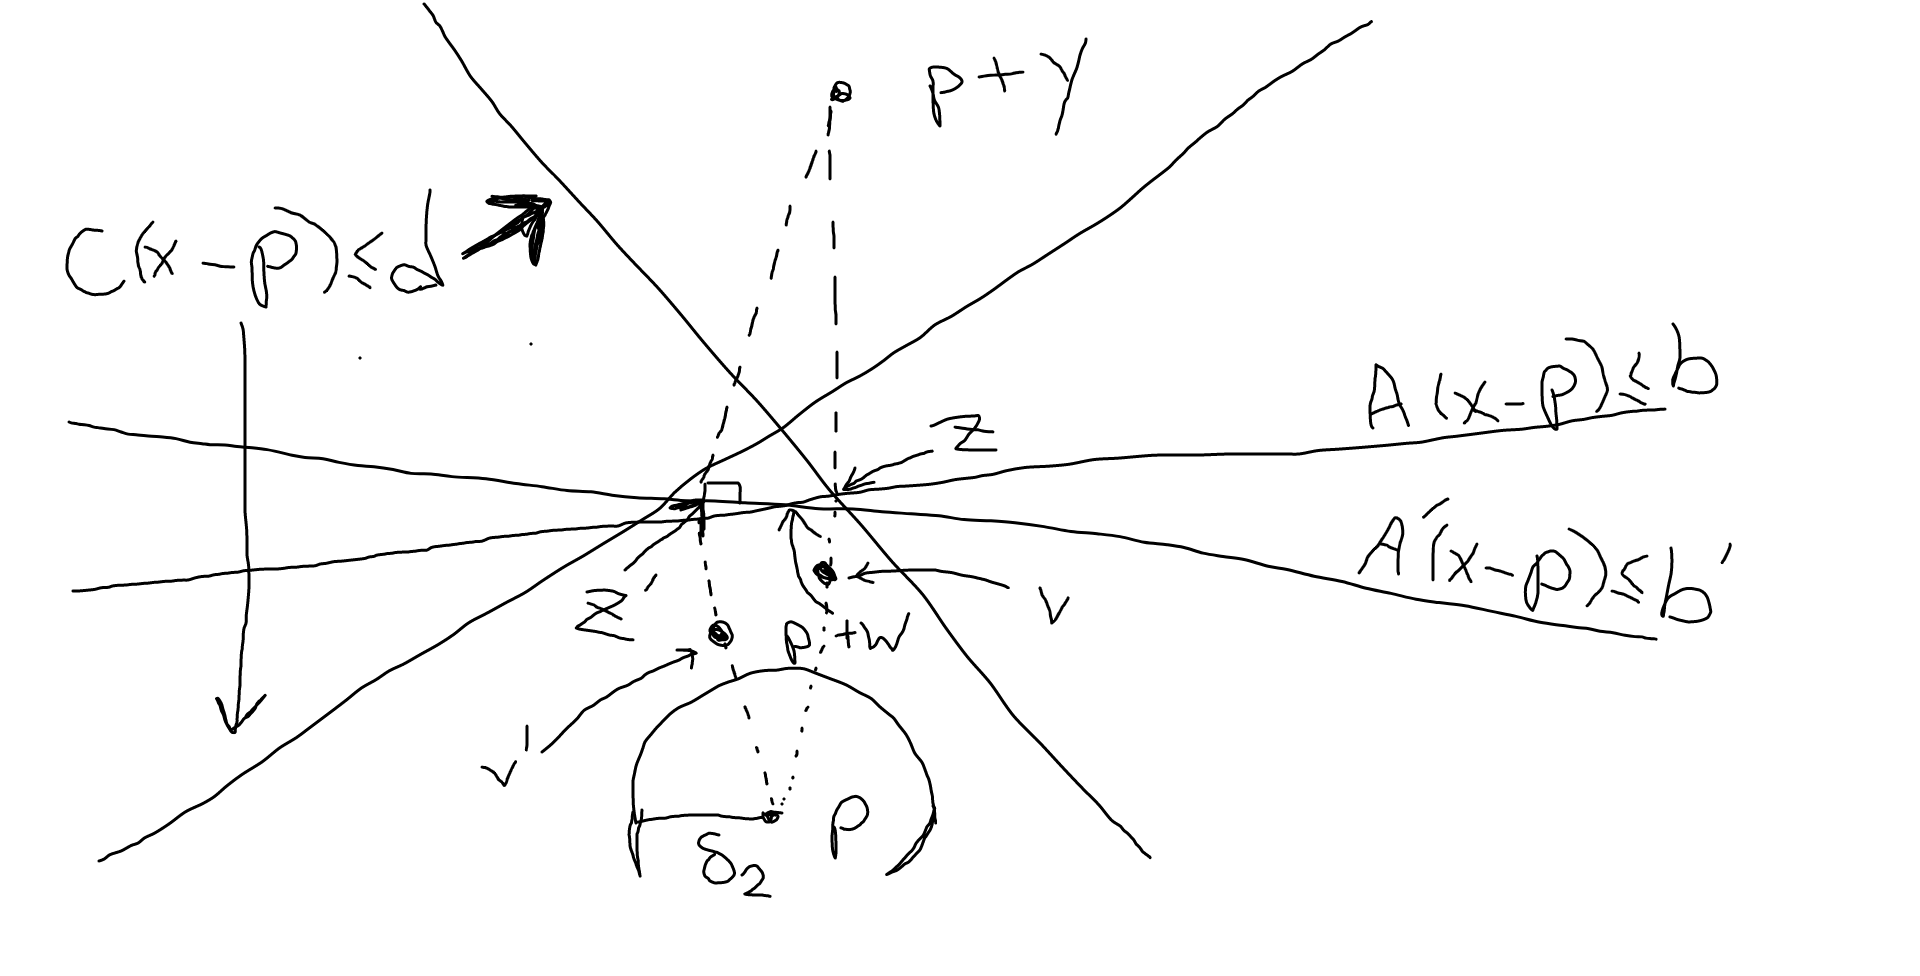
\includegraphics[width=300px]{images/second_lemma.png}
	\caption{
		The constraints $A(x-p) \le b$ are perturbed to $A'(x-p) \le b'$ and do not intersect the sphere of radius $\delta_2$ centered at $p$.
		Then the projections of $p+y$ onto these polyhedra intersected another polyhedra $C(x-p) \le d$ are bounded from eachother.
	}
	\label{second_lemma}
\end{figure}
The following lemma is illustrated in \cref{second_lemma}.


\begin{lemma}
\label{simplified_projections_lemma}
Let
$A, A' \in \mathbb \mathbb R^{m \times n}$;
$b, b' \in \mathbb \mathbb R^{m}_{\ge 0}$;
$C \in \mathbb \mathbb R^{m' \times n}$;
$d \in \mathbb \mathbb R^{m'}_{\ge 0}$;
$p, y \in \Rn$;
$\delta_1, \delta_2, \gamma, \epsilon > 0$;
be given such that
\begin{align*}
\begin{array}{cccccc}
\|A - A'\| \le \epsilon, &
\|b - b'\| \le \epsilon, \\
\delta_1 \le \delta_2 \|A_i\| \le b_i, &
\delta_1 \le \delta_2 \|A'_i\| \le b'_i, \\
\gamma = \frac{2}{\delta_1}\left(1 + \|y\|\right), &
\epsilon \le \min\left\{\gamma^{-1}\right\}.
\end{array}
\end{align*}
Then
\begin{align*}
\|z - z'\| \le \left(2 + \|y\|\right) \gamma \epsilon + 2 \sqrt{2\|y\|\gamma \epsilon}
\end{align*}
where
\begin{align*}
z  = \argmin_{\substack{C(x - p) \le d \\ A (x - p) \le b }} \|p + y - x\| \quad \textrm{and} \quad
z' = \argmin_{\substack{C(x - p) \le d \\ A'(x - p) \le b'}} \|p + y - x\|.
\end{align*}
\end{lemma}
% y - z  =       A        ^T\mu  + C^T\lambda  \\
% y - z' = \left(A'\right)^T\mu' + C^T\lambda' \\

\begin{proof}
% Let $\zeta : \mathbb R^{m \times n} \to \mathbb R^m_+$ be defined by
% \begin{align*}
% \zeta (A) = \begin{pmatrix}
% \|A_1\| \\ \|A_2\| \\ \vdots \\ \|A_m\|
% \end{pmatrix}.
% \end{align*}
Define
\begin{align*}
t' = \max_{\substack{i \in [m] \\ A_i'(z - p) > b_i'}} \frac{A'_i (z - p) - b'_i}{A'_i (z - p)}
\quad \textrm{and} \quad
t = \max_{\substack{i \in [m] \\ A_i(z' - p) > b_i}} \frac{A_i (z' - p) - b_i}{A_i (z' - p)}.
\end{align*}
First, we bound $t$ and $t'$.
Let $i$ be such that $A_i'(z - p) > b_i'$.
Observe
\begin{align*}
A_i'(z - p) - b_i' 
= A_i(z - p) - b_i + (A_i' - A_i)(z - p) + (b_i' - b_i)
\le 0 + \epsilon \|z - p\| + \epsilon = \epsilon (1 + \|z - p\|)
\end{align*}
so that
\begin{align*}
\left|A_i'(z - p)\right| \ge |b_i'| - \left| A_i'(z - p) - b_i'\right| \ge \delta_l\|A_i'\| - \epsilon (1 + \|z - p\|) \ge \delta_l \delta_m - \epsilon \ge \frac 1 2 \delta_l \delta_m\\
\Longrightarrow \frac 1 {\left|A_i'(z - p)\right|} \le \frac 2 {\delta_l \delta_m}.
\end{align*}
Multiplying these, we find
\begin{align*}
\frac{A'_i (z - p) - b'_i}{A'_i (z - p)} \le \frac{2}{\delta_l \delta_m}\epsilon \left[1 + \|z - p\|\right] \le \gamma \epsilon.
\end{align*}
By symmetry, both
$
t \le \gamma \epsilon \le 1
$ and $
t' \le \gamma \epsilon \le 1.
$


% \color{red}
% \begin{align*}
% x \le \frac a 2
% \Longrightarrow a \le 2a - 2x
% \Longrightarrow ax \le 2x(a-x)
% \Longrightarrow \frac x {a - x} \le \frac 2 a x
% \end{align*}
% \color{black}

Also, note that for each $i \in [m]$, if $A_i'(z - p) > b_i'$,
\begin{align*}
t' \ge \frac{A'_i (z - p) - b'_i}{A'_i (z - p)}
\Longrightarrow (1-t') A'_i (z - p) \le b'_i
\end{align*}
%  t A'_i (z - p) \ge A'_i (z - p) - b'_i \\
Because $t' \le 1$, this is also satisfied when $A_i'(z - p) \le b_i'$, 
so that 
\begin{align*}
(1-t') A' (z - p) \le b'
\Longrightarrow
A' \bigg[\big((1-t') z + t'p\big) - p\bigg] \le b'
\end{align*}
% A' \left[(1-t) z - (1 - t)p\right] \le b' \\
with
\begin{align*}
\|(1-t') z + t'p - z\| = t' \|p - z\| \le \gamma \epsilon \|y\|.
\end{align*}

Notice that $C (p-p) \le d$, $A (p-p) \le b$, and $A' (p-p) \le b'$.
Thus, by convexity of linear constraints, and with the definitions
$v = (1-t') z + t'p - p$ and $v' = (1-t) z' + tp - p$
we have established
\begin{align*}
\begin{array}{cccc}
A'v  \le b', & Av  \le b, & Cv  \le d, & \|z  - p - v \| \le \gamma \epsilon \|y\|, \\
A'v' \le b', & Av' \le b, & Cv' \le d, & \|z' - p - v'\| \le \gamma \epsilon \|y\|.
\end{array}
\end{align*}
Define $w$ such that
\begin{align*}
\begin{array}{ccc}
p + w = & \argmin_{x \in \Rn}	& \|p + y - x\|			\\
		& \textrm{s.t.}			& C(x - p) \le d		\\
		& 						& A (x - p) \le b		\\
		& 						& A' (x - p) \le b'		\\
\end{array}.
\end{align*}
We can immediately see by optimality of $w$ that 
$\|y - w\| = \|p + y - p - w\| \le \|p + y - p\| = \|y\|$.
% $\|y - w\| \le \|y - v\|$, 
% and $\|y - w\| \le \|y - v'\|$.
By the definition of $z$ and $z'$ as minimizers over a superset of $w$'s feasible region, we see
$\|y - (z - p)\| = \|p + y - z\| \le \|p + y - p - w\| = \|y - w\|$
and 
$\|y - (z' - p)\| \le \|y - w\|$.
Also by optimality of $w$, we see that 
$(w - y)^T x \ge (w - y)^T(w - y)$ for all $x \in \Rn$ with $C(x - p) \le d$, $A(x - p) \le b$, and $A'(x - p) \le b'$.
In particular, $(w - y)^T v \ge (w - y)^T(w - y)$ and $(w - y)^T v' \ge (w - y)^T(w - y)$.
With the assignment
\begin{align*}
a \gets w - y,			\quad
x \gets	z  - p,			\quad
y \gets	z' - p,			\quad
u \gets v - p,			\quad
v \gets v' - p,			\quad
\epsilon \gets \gamma \epsilon
\end{align*}
we satisfy the assumptions for
\cref{properties_of_a_circle}
and conclude
\begin{align*}
\|z - z'\| = \|z - p - z' + p\|
\le \left(2 + \|w - y\|\right) \gamma \epsilon + 2 \sqrt{2\|w - y\|\gamma \epsilon}
\le \left(2 + \|y\|\right) \gamma \epsilon + 2 \sqrt{2\|y\|\gamma \epsilon}.
\end{align*}
\end{proof}

\color{black}

\subsection{Convergence}
\label{convergence_section}


\subsubsection{Criticallity Goes to Zero, Part 2}
\label{limit_of_criticallity_to_zero}

\begin{criteria}
\label{the_contradiction}
Let $\chik$ be defined by \cref{define_criticality_measure}.
There exists $\epsilon_{\textrm{lb}} > 0$, such that the set 
$\mathcal U = \left\{k \in \naturals | \chik \ge \epsilon_{\textrm{lb}} \right\}$
is infinite.
\end{criteria}

Letting $\epsilon_{lb}$ be defined by \cref{the_contradiction}, as well as the other constants used in \cref{define_reduceiterates},
define
\begin{align}
\Delta_{lb} = \min\left\{
\dsr,
\frac{\epsilon_{lb}}{\maxmodelhessian}, 
\frac{(1-\gammasm)}{\theirc}\epsilon_{lb}, 
\left(\frac 1 {\kappa_{\chi}}  \epsilon_{lb} \right)^{\frac 1 {p_{\Delta}}}, 
1
\right\}. \label{define_delta_lb}
\end{align}


Using the same , \cref{delta_to_zero} implies the existence of $k_0 \in \naturals$ such that for all $k \ge k_0$,

\begin{lemma}
\label{contradiction_portion}
Let $ \epsilon_{\textrm{lb}} $ be defined by \cref{the_contradiction}.

Suppose that 
\cref{bounded_below_assumption}
and the assumptions for
\cref{bounded_model_hessian_lemma}, \cref{liminf_chi_to_zero}, \cref{delta_to_zero}, and \cref{sufficient_reduction_theorem} hold.
Let 
$S_{lb} \subset \naturals \times \naturals$ be the sequence
\begin{align}
\label{define_slb}
S_{lb} = \left\{\left(k,
\min_{i \in \naturals, i > k, \chi_{i} \le \epsilon_{\textrm{lb}}} i
\right)\right\}_{k=1}^{\infty}.
\end{align}

If \cref{the_contradiction} were true, then the sequence $S_{lb}$ satisfies \cref{criteria_from_contradiction}.
\end{lemma}
\begin{proof}
Notice that \cref{liminf_chi_to_zero} ensures that the sequence $S_{lb}$ is well defined.
By \cref{delta_to_zero}, there exists $k_1 \in \naturals$ such that if $k \ge k_1$, then $\dk \le \Delta_{lb}$ as defined in \cref{define_delta_lb}.
Let $\suffiterates$ be defined by \cref{define_suffiterates}, and consider
$C_k = \left\{i \in \suffiterates | k_1 \le k \le i < l \right\}$ for $(k, l) \in S_{lb}$.
Note that $k \in \suffiterates$, so $C_k \ne \emptyset $.
For each $i \in C_k$, using the fact that $i \in \suffiterates$, \cref{bounded_model_hessian_lemma}, and \cref{sufficient_reduction_theorem}, we can conclude
\begin{align*}
f\left(x^{(i)}\right) - f\left(x^{(i+1)}\right) 
\ge \gammabi \left( \mfk\left(x^{(i)}\right) - \mfk\left(x^{(i)} + s^{(i)}\right) \right) 
\ge \gammabi \kappa_f \chi_i \min\left\{\frac{\chi_{i}}{\maxhessian}, \Delta_i, 1\right\} 
\end{align*}

By the definition of $l$, we have that $\chi_i > \frac{\epsilon_{lb}}{2}$ for all $i \in C_k$.
As $i \ge k$, we have $\Delta_i \le \frac{\epsilon_{lb}}{\maxhessian}$ and $\Delta_i \le 1$.
Therefore,
\begin{align*}
\frac{\Delta_i}{2} \le \frac{\epsilon_{lb}}{2 \maxhessian} \le \frac{\chi_i}{\maxhessian}.
\end{align*}

It follows that
\begin{align*}
f\left(x^{(i)}\right) - f\left(x^{(i+1)}\right) > \frac{\gammabi \kappa_f \epsilon_{lb} \Delta_i}{4}
\end{align*}

and hence
\begin{align*}
\Delta_i < \frac{4}{\gammabi \kappa_f \epsilon_{lb}} \left[ f\left(x^{(i)}\right) - f\left(x^{(i+1)}\right)\right].
\end{align*}

Meanwhile,
\begin{align*}
\left\|\xk - \xl\right\| \le \sum_{i \in C_k}\left\|x^{(i)} - x^{(i+1)}\right\| \le \sum_{i \in C_k} \Delta_i
\end{align*}
so that

\begin{align}
\left\|\xk - \xl\right\| < \frac{4}{\gammabi \kappa_f \epsilon_{lb}} \left[ f\left(\xk\right) - f\left(\xl\right)\right].
\end{align}

We also know that $\left\{f\left(\xk\right)\right\}$ is bounded below by \cref{bounded_below_assumption}, 
and since it is nonincreasing, $f\left(\xk\right)  - f\left(\xl\right) \to 0$.
Therefore $\left\{\left\|\xk - \xl\right\|\right\}_{k \in S_{lb}}$ converges to zero.
\end{proof}


\begin{lemma}
\label{lim_chi_to_zero}

Let $\chik$ be defined by \cref{define_criticality_measure}.
Suppose that 
\cref{lipschitz_gradients_assumption}
the assumptions for 
\cref{delta_to_zero},
\cref{contradiction_portion},
\cref{liminf_chi_to_zero}.
hold.
If $\gammabi > 0$, then $\lim_{k\to\infty}\chik=0$.
\end{lemma}


\begin{proof}
Suppose for a contradiction that \cref{the_contradiction} were true, and $\mathcal U = \left\{k \in \naturals | \chik \ge \epsilon_{\textrm{lb}} \right\}$ is infinite.
By \cref{delta_to_zero}, there exists $k_1 \in \naturals$ such that if $k \ge k_1$, then $\dk \le \Delta_{lb}$ as defined in \cref{define_delta_lb}.
Then, if $k \in \mathcal U$ with $k \ge k_0$, then $k \in \reduceiterates \subset \miniterates$.
% \begin{align*}
% \dk \le \min\{\frac{\chik}{\maxhessian}, \frac{(1-\gammasm)\chik}{c}, \left(\frac 1 {\kappa_{\chi}}  \epsilon \right)^{\frac 1 {p_{\Delta}}}, 1\}
% \end{align*}
% and therefore $k \in \miniterates \subset S$.

Let $(k, l) \in S_{lb}$ defined by \cref{define_slb} be given with $k \ge k_1$.
This means that $\chik - \chi^{(l)} \ge \frac {\epsilon} 2 $.

We know by \cref{lipschitz_gradients_assumption} and \cref{accuracy_is_satisfied} that there is a $\kappa_g > 0$ and $\lipgrad>0$ such that
\begin{align}
\left\|\gk - \gl\right\| \nonumber \\
\le \left\|\gk - \gradf\left(\xk\right)\right\| 
+ \left\|\gradf\left(\xk\right) - \gradf\left(\xl\right)\right\| 
+ \left\|\gradf\left(\xl\right) - \gl \right\| \nonumber \\
\le \kappa_g \left(\dk^2 + \dl^2\right) + \lipgrad \left\|\xk - \xl \right\| \label{chi2zero2_comp1}
\end{align}


% Let $\zmk$, $\zlk$, $\zck$ be defined by \cref{define_zmk}, \cref{define_zlk}, \cref{define_zck} respectively.
Let $\zmk$ and $\zlk$ be defined by \cref{define_zmk} and \cref{define_zlk} respectively.
Using the triangle inequality, the contraction property of projections, 
\cref{define_criticality_measure}, and \cref{chi2zero2_comp1} we have 
\begin{align*}
\frac{\epsilon}{2} \le \chik - \chi^{(l)} \\
=     \left\|P_{\feasiblek}\left(\xk - \gk\right) - \xk\right \| 
    - \left\|P_{\feasiblel}\left(\xl - \gl\right) - \xl\right \| \\
\le   \left\|P_{\feasiblek}\left(\xk - \gk\right) - \xk
    -  P_{\feasiblel}\left(\xl - \gl\right) + \xl\right \| \\
 \le  \left\|\xk - \xl\right\|
 + \left\|P_{\feasiblek}\left(\xk - \gk\right) -  P_{\feasiblel}\left(\xk - \gk\right) \right\| \\
 + \left\|P_{\feasiblel}\left(\xk - \gk\right) -  P_{\feasiblel}\left(\xl - \gl\right) \right\| \\
\le \left\|\xk - \xl\right\| + \left\|\zmk - \zlk\right\| 
+ \left\| \xk - \gk - \xl + \gl  \right\| \\
\le \left(2 + \lipgrad\right) \left\|\xk - \xl\right\| 
+ \kappa_g \left(\dk^2 + \dl^2\right)
+ \left\|\zmk - \zlk\right\|
\end{align*}
        
% \begin{align*}
% \le\left\|\xk - x^{(l_k)}\right\| + \| p^{(k\to k)} - p^{(k\to l)}\| + \left\|\xk - \gk - x^{(l_k)} - {\nabla m_f^{(l_k)}\left(x^{(l_k)}\right)}\right\| \\
% \le 2\left\|\xk - x^{(l_k)}\right\| + \| p^{(k\to k)} - p^{(k\to l)}\| + \left\|\gk - {\nabla m_f^{(l_k)}\left(x^{(l_k)}\right)}\right\|\\
% =   (2 + \lipgrad) \left\|\xk - x^{(l_k)}\right\| + \| p^{(k\to k)} - p^{(k\to l)}\| + \kappa_g \left(\dk^2 + \Delta_{l_k}^2\right)
% \end{align*}


% \le 2\left\|\xk - x^{(l_k)}\right\| + \| p^{(k)} - p^{(k_l)}\| + \left\|\gk - \gradf(\xk)\right\| + \left\|\gradf(\xk) - \gradf(x^{(l_k)})\right\| + \left\|\gradf(x^{(l_k)}) - {\nabla m_f^{(l_k)}\left(x^{(l_k)}\right)}\right\| \\
% \le \left(2 + \lipgrad\right)\left\|\xk - x^{(l_k)}\right\| + \| p^{(k)} - p^{(k_l)}\| + \left\|\gk - \gradf(\xk)\right\| + \left\|\gradf(x^{(l_k)}) - {\nabla m_f^{(l_k)}\left(x^{(l_k)}\right)}\right\|.
% \le\left\|\xk - x^{(l_k)}\right\| +  \left\|P_{\Omega_1}\left(\xk - \gk\right) - P_{\Omega_2}\left(x^{(l_k)} - g^{(l_k)}\right)\right\| \\

So that
\begin{align}
\frac{\epsilon_{lb}} 2 \le \left(2 + \lipgrad\right) \left\|\xk - \xl\right\| 
+ \kappa_g \left(\dk^2 + \dl^2\right)
+ \left\|\zmk - \zlk\right\|
\label{chi2zero2_conv}.
\end{align}

Because we have assumed \cref{the_contradiction}, we can apply \cref{contradiction_portion} so that 
$S_{lb}$ defined \cref{define_slb} satisfies \cref{criteria_from_contradiction}.
We can then apply \cref{bounded_projection_theorem} and \cref{delta_to_zero} to conclude that the entire right hand side of \cref{chi2zero2_conv} goes to zero.
This is a contradiction, and \cref{the_contradiction} must be false.
\end{proof}

\subsubsection{Convergence of Criticallity Measure}
\label{limit_of_true_criticallity}

\begin{theorem}
\label{the_convergence_theorem}
Suppose that \cref{lipschitz_gradients_assumption}, \cref{bounded_below_assumption}, \cref{bounded_hessians_assumption}, and 
the assumptions for \cref{accuracy_is_satisfied} hold.

If $\gammabi = 0$, then
\begin{align}
\liminf_{k\to\infty} \left\|P_{\feasible}\left(\xk - \gradf\left(\xk\right)\right) - \xk \right\| = 0.
\end{align}

If $\gammabi > 0$, then
\begin{align}
\lim_{k\to\infty} \left\|P_{\feasible}\left(\xk - \gradf\left(\xk\right)\right) - \xk \right\| = 0.
\end{align}

\end{theorem}



\begin{proof}
Let 
$\feasiblek$, $\zmk$, $ \truefeasiblek $, $\zck$
be defined by 
\cref{define_feasiblek}, \cref{define_zmk}, \cref{sha_truefk}, \cref{define_zck}
respectively.
Let $\epsilon > 0$ be fixed.
By the triangle inequality, the contraction property of projections, we have
\begin{align*}\left \|
 P_{\truefeasiblek}\left(\xk - \gradf\left(\xk\right)\right)
-P_{\feasiblek}\left(\xk - \gk \right)
\right\| 
\le 
\bigg \|
 P_{\truefeasiblek}\left(\xk - \gradf\left(\xk\right)\right) \\
-P_{\truefeasiblek}\left(\xk - \gk \right)
+P_{\truefeasiblek}\left(\xk - \gk \right)
-P_{\feasiblek}\left(\xk - \gk \right)
\bigg\| \\
\le \left\|
\xk - \gradf\left(\xk\right) - \xk + \gk
\right\| + \left\|\zck - \zmk\right\| \\
\le \left\|\gk - \gradf\left(\xk\right)\right\| + \left\|\zck - \zmk\right\|
\end{align*}
With $\chik$ defined by \cref{define_criticality_measure}, the triangle inequality implies
\begin{align*}
\left\|P_{\truefeasiblek}\left(\xk - \gradf\left(\xk\right)\right) - \xk \right\| \\
= \left\|
 P_{\truefeasiblek}\left(\xk - \gradf\left(\xk\right)\right)
-P_{\feasiblek}\left(\xk - \gk \right)
+P_{\feasiblek}\left(\xk - \gk \right)
- \xk\right\| \\
\le \left\|\gk - \gradf\left(\xk\right)\right\| + \left\|\zck - \zmk\right\| + \chik.
\end{align*}
\end{proof}
Using \cref{delta_to_zero}, \cref{accuracy_is_satisfied}, \cref{bounded_projection_theorem}, 
there is a $k_0$ such that if $k \ge k_1$, then
\begin{align*}
\left\|\gk - \gradf\left(\xk\right)\right\| \le \kappa_g \dk^2 \le \frac 1 2 \epsilon
\quad \textrm{and} \quad
\left\|\zck - \zmk\right\| \le \frac 1 2 \epsilon
\end{align*}
so that
\begin{align*}
\lim_{k\to\infty} \left[\left\|\gk - \gradf\left(\xk\right)\right\| + \left\|\zck - \zmk\right\|\right] = 0.
\end{align*}


The result follows from \cref{liminf_chi_to_zero}, \cref{lim_chi_to_zero} and convexity:
\begin{align*}
\left\|P_{\feasible}\left(\xk - \gradf\left(\xk\right)\right) - \xk \right\| 
\le \left\|P_{\truefeasiblek}\left(\xk - \gradf\left(\xk\right)\right) - \xk \right\|.
\end{align*}

\subsection{Bounded Level Sets}
\label{bounded_level_sets}

We would have been able to make a number of simplifications if we assume bounded level sets.


\begin{assumption}
\label{bounded_level_sets}
All level sets of the function $f$ are bounded. That is, for each $r \in \reals$, there exists an $M$ such that 
\begin{align*}
\|y\| \le M \quad \forall y \in \Omega \quad \textrm{s.t.} \quad f(y) = r.
\end{align*}
\end{assumption}

% Notice that \cref{bounded_level_sets}





\section{Future Work}
\subsection{Removing a regularity assumption}
\label{alternative_assumptions_section}

We have made \cref{minangleassumption_alt}, which is an assumption about the constraint's models.
We would have preferred to make an assumption about the true constraints: \cref{minangleassumption_alt}.
However, the boundededness of the ellipsoids according to \cref{ellipsoids_notation_definitions} shown in \cref{bounded_condition_numbers}
is required to show prove \cref{accuracy_is_satisfied}.
Yet, \cref{accuracy_is_satisfied} is key to applying results about true constraints to results about their models.
In this section, we discuss some progress towards replacing \cref{minangleassumption} with \cref{minangleassumption_alt}.
In the process, we are also able to remove \cref{mingradassumption}.






\begin{definition}
Let $\epsilon > 0$ be a given constant.
A constraint $c_i(x) \le 0$ is said to be $\epsilon$-nearly active at $x \in \feasible$ if $|c_i(x)| \le \epsilon$.
\end{definition}

\begin{definition}
Let $\epsilon > 0$ be given.
Define the set of indices of $\epsilon$ active constraints at a point $x \in \feasible$ by
\begin{align}
\epsactive(x; \epsilon) = \bigg\{ i \in [m] \bigg | |c_i(x)| \le \epsilon \bigg\} \label{define_epsactive}
\end{align}
\end{definition}

\begin{definition}
Let $\epsilon > 0$ be given.
Define the set of indices of $\epsilon$ active model constraints at a point $x \in \feasible$ by
\begin{align}
\epsactivemodels(x; \epsilon) = \bigg\{ i \in [m] \bigg | |m_{c_i}(x)| \le \epsilon  \bigg\} \label{define_epsactivemodels}
\end{align}
\end{definition}

\begin{assumption}
\label{minangleassumption_alt_func}
There exists a $\minanglealpha$ and $\epsilon > 0$ such that for every $x \in \feasible$, 
there is a unit vector $\minanglediralt(x)$ such that
\begin{align*}
\nabla c_i(x)^T\minanglediralt(x) > \minanglealpha\quad \forall i \in \epsactive(x; \epsilon).
\end{align*}
\end{assumption}


\begin{lemma}
\label{mingradlemma}
Suppose that 
\cref{minangleassumption_alt} holds.
There exist $\mingradepsilon > 0$ and $\mingrad > 0$ such that for each $x \in \Omega$ we have
\begin{align*}
\| \nabla c_i(x) \| \ge \mingrad \quad \forall i \in \epsactive(x; \mingradepsilon).
\end{align*}
\end{lemma}
\begin{proof}
Let $x \in \Omega$ be arbitrary.
By \cref{minangleassumption_alt} we know there are some constants $\minanglealpha>0$ and $\epsilon>0$ and unit vector $\minanglediralt(x)$ such that for all $i \in \epsactive(x; \epsilon)$,
$\nabla c_i(x)^T\minanglediralt(x) \ge \minanglealpha$.
Letting $\mingradepsilon = \epsilon$ and $\mingrad = \minanglealpha$, we see that for all $i \in \epsactive(x; \mingraddelta)$,
\begin{align*}
\|\nabla c_i(x)\| = \|\nabla c_i(x)\| \|\minanglediralt(x)\| \ge \nabla c_i(x)^T\minanglediralt(x) \ge \minanglealpha = \mingrad.
\end{align*}
\end{proof}

The following result is close to showing a bound the condition numbers of $\qk$.
However, it relies on $\dk \to 0$.
\begin{lemma}
Suppose \cref{minangleassumption_alt}
and the assumptions for \cref{accuracy_is_satisfied_lemma} and \cref{bounded_gradients_lemma} are satisfied.
There exists $\dacc > 0$ and $\sigma_0 \ge 1$ such that if $\dk \le \dacc$, and
\begin{align}
\sigma\left( Q^{(k-1)} \right) \le \sigma_0 \label{idk_alt_proof_statement1}
\end{align}
then 
\begin{align}
\sigma\left( \qk \right) \le \sigma_0. \label{idk_alt_proof_statement2}
\end{align}
\end{lemma}


\begin{proof}
Let $\epsilon, \minanglealpha > 0$ be defined by \cref{minangleassumption_alt}, and $\maxgrad$ be defined by \cref{bounded_gradients_lemma}.
Define
\begin{align}
&M = \frac 1 {\maxgrad + \frac 1 2 \minanglealpha} & \\
&\textrm{and} \quad \sigma_0 = \max\left\{1, \frac{48}{M^2\left(\minanglealpha\right)^2}\right\}.&
\end{align}
By \cref{boundbeta}, there exists $\dacco \left(\frac {M \minanglealpha} 2\right) > 0$ such that if
$\thetamink \ge \frac {M \minanglealpha} 2$ and $\dk \le \dacco \left(\frac {M \minanglealpha} 2\right)$,
then $\sigma\left(\qk\right) \le \frac{12}{\left(\frac{M\minanglealpha}{2}\right)^2} = \sigma_0$.
Define 
\begin{align}
\dacc = \min\left\{
\dacco \left(\frac {M \minanglealpha} 2\right), 
\sqrt{\frac {\minanglealpha}{2\kappa_g\sqrt{\sigma_0}}},
\frac{M \epsilon}{\sqrt{n}}
\right\} \label{define_delta_accuracy2}
\end{align}
and suppose that \cref{idk_alt_proof_statement1} and $\dk \le \dacc$ hold.
By \cref{boundbeta}, \cref{idk_alt_proof_statement2} follows from $\thetamink \ge \frac {M \minanglealpha} 2$.

% then
% \begin{align}
% \sqrt{\sigma\left(\qk \right)} \le \frac{48}{M^2\left(\minanglealpha\right)^2}
% \end{align}
% Suppose that $\epsactive(\xk; \epsilon) = \emptyset$.
% for all $y \in \tr$, we have
% \begin{align*}
% \left\|\gradf\left(y\right) - \nabla \mfk\left(y\right) \right\| \le \kappa_g \sqrt{\sigma\left( Q^{(k-1)} \right)}\dk^2.
% \end{align*}
% In particular, there exists $u \in \Rn$ with $\|u\| \le 1$ such that

By \cref{accuracy_is_satisfied_lemma}, there exists $\kappa_{g} > 0$ and $u\in\Rn$ with $\|u\|\le 1$ such that
\begin{align}
\nabla c_i\left(\xk\right) = \gmcik + \kappa_g \sqrt{\sigma\left( Q^{(k-1)} \right)}\dk^2 u. \label{idk_alt_proof_eqn2}
\end{align}
Taking the square root of \cref{idk_alt_proof_statement1} and multiplying by $\dk^2 \le \frac {\minanglealpha}{2\kappa_g\sqrt{\sigma_0}}$, we see
\begin{align}
\sqrt{\sigma\left( Q^{(k-1)} \right)} \dk^2 \le \frac {\minanglealpha} {2\kappa_g}. \label{idk_alt_proof_ass1}
\end{align}
We see that by the triangle inequality, \cref{bounded_gradients_lemma}, \cref{idk_alt_proof_eqn2}, and \cref{idk_alt_proof_ass1} that
\begin{align}
\left\|\gmcik\right\| \le \left\| \nabla c_i\left(x\right)\right\| + \kappa_g \sqrt{\sigma\left( Q^{(k-1)} \right)} \dk^2 \le \maxgrad + \frac 1 2 \minanglealpha = \frac 1 M \nonumber \\
\Longrightarrow \frac 1 {\left\|\gmcik\right\|} \ge M. \label{idk_alt_proof_eqn4}
\end{align}

Let $\activeconstraintsk$ and $\epsactive(x; \epsilon)$
% and $\epsactivemodels(x; \epsilon)$
be defined by
\cref{define_activeconstraints} and \cref{define_epsactive}
% , and \cref{define_epsactivemodels}
respectively.
If $\activeconstraintsk = \emptyset$, then $\sigma\left(\qk\right) = 1$.
Otherwise, let $i \in \activeconstraintsk$ be arbitrary,
so that $\zik \in \tr$. By \cref{define_z}
\begin{align*}
M \left|m_{c_i}\left(\xk\right)\right| \le \frac{\left|m_{c_i}\left(\xk\right)\right|}{\left\|\gmcik\right\|} \le \sqrt{n} \dk \Longrightarrow
\left|c_i\left(\xk\right)\right| \le \frac{\sqrt{n}\dk}{M} \le \epsilon
\end{align*}
by \cref{define_delta_accuracy2}.
This means that $i \in \epsactive(\xk; \epsilon)$, so that by \cref{minangleassumption_alt} there exists a unit vector $\minanglediralt(\xk)$ with
\begin{align}
\nabla c_i\left(\xk\right)^T\minanglediralt\left(\xk\right) > \minanglealpha \label{idk_alt_proof_eqn1}
\end{align}
Substituting \cref{idk_alt_proof_eqn2} into \cref{idk_alt_proof_eqn1} yields:
\begin{align*}
\left(\gmcik + \kappa_g \sqrt{\sigma\left( Q^{(k-1)} \right)}\dk^2 u\right)^T \minanglediralt(x) > \minanglealpha
\end{align*}
Using \cref{idk_alt_proof_ass1}, $\|u\|\le 1$, and $\|\minanglediralt(x)\| = 1$, this becomes
\begin{align}
\gmcik^T\minanglediralt(x) > \minanglealpha - \kappa_g \sqrt{\sigma\left( Q^{(k-1)} \right)}\dk^2 u^T\minanglediralt(x) \ge \frac 1 2 \minanglealpha \label{idk_alt_proof_eqn3}
\end{align}
Multiplying \cref{idk_alt_proof_eqn3} and \cref{idk_alt_proof_eqn4} yields
\begin{align}
\frac{\gmcik}{\left\|\gmcik\right\|}^T  \minanglediralt(x) \ge \frac M 2 \minanglealpha. \label{idk_alt_proof_eqn5}
\end{align}
Let $\huk$ be defined by \cref{define_u}, 
% \begin{align*}
% \huk \in -\argmin_{\|u\| = 1} \max_{i \in \activeconstraintsk} u^T \frac{\gmcik}{\left\|\gmcik\right\|}
% \end{align*}
and $\thetamink$ be defined by \cref{define_thetamink}.
Then \cref{idk_alt_proof_eqn5} tells us 
\begin{align*}
\thetamink = \min_{i \in \activeconstraintsk} \left(-\hgik\right)^T \huk \ge \frac{\gmcik}{\left\|\gmcik\right\|}^T \minanglediralt(x) \ge \frac M 2 \minanglealpha.
\end{align*}
% Then by \cref{boundbeta}, there exists $\dacc(\epsilon) > 0$ such that if $\thetamink >$
% \begin{align*}
% \sigma\left(\qk\right) \le \frac{48}{M^2\left(\minanglealpha\right)^2}
% \end{align*}
% Now,
% \begin{align*}
% \sigma_2 = \frac{\max\left\{1, \frac{\beta^2}{1 - \beta^2}\right\}}{\min\left\{1, \frac{\beta^2}{1 - \beta^2}\right\}}
% \end{align*}

% We know that the next trial point $\xkpo$ must also lie within the trust region, so that we have both
% \begin{align*}
% \left\|\gradf\left(\xk\right) - \nabla \mfk\left(\xk\right) \right\| \le \kappa_g \sqrt{\sigma_1}\dk^2 \\
% \left\|\gradf\left(\xkpo\right) - \nabla \mfk\left(\xkpo\right) \right\| \le \kappa_g \sqrt{\sigma_1}\dk^2 \\
% \end{align*}
% 
% \begin{align*}
% \nabla \mfk\left(\xk\right)  = \gradf\left(\xk\right) + \kappa_g \sqrt{\sigma_1}\dk^2 \\
% \end{align*}
% 
% 
% 
% Let $\bsk$ be defined by \cref{define_bsk}.
% Let $\alpha$ and $\beta$ be defined by \cref{define_alpha_beta}.
% Let $p_{\alpha}$ and $p_{\beta}$ be defined by \cref{define_p_alpha} and \cref{define_p_beta} respectively.
% \begin{align}
% \end{align}
% 
% \begin{align*}
% \huk \in -\argmin_{\|u\| = 1} \max_{i \in \activeconstraintsk} u^T \frac{\gmcik}{\left\|\gmcik\right\|} \\
% \bsk = \beta\dk^{p_{\beta}} + \sqrt{\left(1 - \left(\beta\dk^{p_{\beta}}\right)^2\right)\left(1 - \left(\thetamink\right) ^2\right)} \\
% \end{align*}
\end{proof}



\color{red}
\begin{lemma}
\label{minanglelemmap2}
Suppose that \cref{minangleassumption_alt}, \cref{max_norm_assumption}, and \cref{lipschitz_gradients_assumption} hold.
There exists $\minangledelta > 0$ and $\minanglealpha > 0$ such that for each $x \in \feasible$, there is a unit vector $\minangledir(x)$ such that
if $\dk \le \minangledelta$ and $i$ is such that $\zik \in B_{\infty}(\xk, \dk)$
then
\begin{align*}
-\frac {\gmcik}{\|\gmcik\|} ^T\minangledirk \ge \minanglealpha.
\end{align*}
Without loss of generality, $\minanglealpha \le \frac 1 2$.
\end{lemma}
\begin{proof}
By \cref{minanglelemmap1}, there exist $\minangledelta' > 0$ and $\minanglealpha'$ such that for each $x \in \feasible$, 
there is a unit vector $\minangledir'(x)$ such that
\begin{align*}
-\frac {\nabla c_i(x)}{\|\nabla c_i(x)\|}^T \minangledir'(x) \ge \minanglealpha'
\Longrightarrow -\nabla c_i(x)^T \minangledir'(x) \ge \minanglealpha' \|\nabla c_i(x)\|
\end{align*}

\begin{comment}
Need to show:
\begin{align*}
-\frac {\nabla c_i(x)}{\|\nabla c_i(x)\|}^T \minangledir'(x) \ge \minanglealpha' \Longrightarrow -\frac {\gmcik}{\|\gmcik\|} ^T\minangledirk \ge \minanglealpha
\end{align*}
and
\begin{align*}
\zik \in B_{\infty}(\xk, \dk) \Longrightarrow i \in \epsactivemodels(x, \minangledelta)
\end{align*}


\begin{align*}
\zik \in B_{\infty}(\xk, \dk) \\
\Longrightarrow \|\zik - \xk\| \le \sqrt{n}\dk \\
\Longrightarrow \left\|\frac{m^{(k)}_{c_i}(\xk)}{\left\|\gmcik\right\|^2} \gmcik\right\| \le \sqrt{n}\dk \\
\Longrightarrow \frac{|m^{(k)}_{c_i}(\xk)|}{\left\|\gmcik\right\|}  \le \sqrt{n}\dk \\
\Longrightarrow i \in \epsactivemodels(x, \minangledelta)
\end{align*}

\end{comment}
\end{proof}
\color{black}



\color{red}
\begin{lemma}
\label{minanglelemmap1}
Suppose that \cref{minangleassumption_alt}, \cref{max_norm_assumption}, and \cref{lipschitz_gradients_assumption} hold.
There exists $\minangledelta > 0$ and $\minanglealpha$ such that for each $x \in \feasible$, there is a unit vector $\minangledir(x)$ such that
\begin{align*}
-\frac {\nabla c_i(x)}{\|\nabla c_i(x)\|}^T \minangledir(x) \ge \minanglealpha.
\end{align*}
\end{lemma}
\begin{proof}
By \cref{bounded_gradients_lemma}, there exists $\maxgrad$ with $\|\nabla c_i(x) \| \le \maxgrad$ for any $x \in \feasible$.
Let \cref{minangleassumption_alt} hold with constants $\minanglealpha'$ and $\epsilon$, so that for any $x \in \feasible$, there is a unit vector $\minanglediralt(x)$ with
\begin{align*}
\nabla c_i(x)\minanglediralt(x) \ge \minanglealpha'.
\end{align*}
Also, by \cref{mingradlemma}, there exist $\mingradepsilon > 0$ and $\mingrad > 0$ such that for each $x \in \Omega$ we have
\begin{align*}
\| \nabla c_i(x) \| \ge \mingrad \quad \forall i \in \epsactive(x; \mingradepsilon).
\end{align*}
By letting $\minangledir(x) = -\minanglediralt(x)$, $\minanglealpha = \minanglealpha'\maxgrad$, $\minangledelta = \min\{\epsilon, \minangledelta\}$, 
we see that for all $x \in \feasible$ and $i \in \epsactive(x; \minangledelta)$,
\begin{align*}
-\nabla c_i(x) \minanglediralt(x) \ge \minanglealpha'\maxgrad \ge \minanglealpha'\|\nabla c_i(x)\|.
\end{align*}
Now, because $\| \nabla c_i(x) \| \ge \mingrad > 0$, we can divide by $\| \nabla c_i(x) \|$ to find
\begin{align*}
-\frac {\nabla c_i(x)}{\|\nabla c_i(x)\|}^T \minangledir(x) \ge \minanglealpha.
\end{align*}
\end{proof}
\color{black}


\subsection{Removing the Hoffman assumption}
\label{removing_the_huffman_assumption}



\subsubsection{Just removed...}

In order to show that the hoffman constant is bounded across iterations, we make the following additional assumption.
We leave removing this assumption as future work, which is discussed in \cref{removing_the_huffman_assumption}.

% \begin{align}
% \nearlyactiveprojk \left(x, y; \epsilon\right) = \left\{ i \in [m] 
% \quad \bigg| \quad
% \left|c_i\left(x\right) + \nabla c_i\left(x\right)^T \left(P_{\truefeasible\left(x\right)}\left(y\right) - x\right)\right| \le \epsilon \right\} \label{sha_nearly_proj_indices}
% \end{align}

% \begin{lemma}
% Suppose that
% \begin{align*}
% b_1 + a_1^T\left(p_1 - x\right) = 0 \\
% b_2 + a_2^T\left(p_2 - x\right) = 0
% \end{align*}
% where 
% \begin{align*}
% \left|b_1 - b_2\right| \le \epsilon
% \quad \textrm{and} \quad
% \left|a_1 - a_2\right| \le \epsilon
% \quad \textrm{and} \quad
% \left|p_1 - p_2\right| \le L.
% \end{align*}
% Then
% \begin{align*}
% b_2 + a_2^T\left(p_2 - x\right) \le \epsilon
% \end{align*}
% 
% \end{lemma}
% \begin{proof}
% 
% 
% \begin{align*}
% \left|c_i\left(\xk\right) + \nabla c_i\left(\xk\right)^T \left(P_{\truefeasible\left(\xk\right)}\left(\xk\right) - \xk\right)\right| \le \epsilon.
% \end{align*}
% 
% \end{proof}

\newpage


\begin{assumption}
\label{huffman_assumption}
There exist $\huffeps, \huffalpha > 0$ such that
for each $x \in \Omega$ and unit vector $y \in \Rn$,
there exists a unit vector $\huffdir(x, y) \in \Rn$ such that
if $i \in [m]$ is such that 
\begin{align*}
y^T \nabla c_i \left(x\right) \ge - \huffeps
\end{align*}
then
\begin{align*}
\huffdir(x, y)^T \nabla c_i \left(x\right) \ge \huffalpha.
\end{align*}
\end{assumption}


Define
\begin{align}
\mathbb J(x, \Delta) = \left\{i \in [m] \bigg | \exists y \in B_{\infty}\left(x, \Delta\right) \quad \textrm{s.t.} \quad c_i(y) \ge 0\right\}.
\end{align}


\begin{assumption}
\label{new_huffman_assumption}
There exist $\huffeps, \huffalpha > 0$ such that
for each $x \in \Omega$,
there exists a unit vector $\huffdir(x) \in \Rn$ such that
\begin{align*}
\huffdir(x)^T \nabla c_i \left(x\right) \ge \huffalpha \quad \forall i \in \mathbb J(x, \huffeps).
\end{align*}
\end{assumption}


\begin{lemma}
% \activeprojkk \cup \activeprojkl \cup \trueactiveprojk
We have that 
\begin{align*}
\activeconstraintsk \cup \activeconstraintsl \subseteq \mathbb J\left(\xk, \max\left\{\sqrt{n}\dk, \left\|\xk - \xl\right\| + \dl\right\}\right) 
\end{align*}
\end{lemma}
\begin{proof}

By \cref{accuracy_is_satisfied}, there exists a $u \in \Rn$ with $\|u\| \le 1$ such that
\begin{align*}
\nabla c_i\left(\xk\right) \le \gmcik + \kappa_f \dk^2 u.
\end{align*}
\begin{comment}
That one had assumptions...
\end{comment}
By \cref{mingradassumption}, there exists $\maxmodelgrad$ such that
\begin{align*}
\left\|\gmcik\right\| \ge \mingrad
\Longrightarrow  \frac{1}{\left\|\gmcik\right\|} \ge \frac 1 {\maxmodelgrad}
\end{align*}

Let $\gamma = \left[1 + \frac{\kappa_f \dk^2}{\left\|\gmcik\right\|}\right]^{-1}$.


If $k \in \activeconstraintsk$, then $\left\|\zik - \xk\right\|_{\infty} \le \dk$.
Using \cref{define_z},


By \cref{constraints_are_convex}, 
\begin{align*}
c_i\left(\xk + \gamma\left(\zik - \xk\right) \right) \ge c_i\left(\xk\right) + \gamma\nabla c_i\left(\xk\right)^T\left(\zik - \xk\right) \\
= c_i\left(\xk\right) - \gamma\frac{c_i\left(\xk\right)}{\left\|\gmcik\right\|^2} \left[\gmcik + \kappa_f \dk^2 u \right]^T\gmcik \\
\ge c_i\left(\xk\right) - \gamma c_i\left(\xk\right)\left[1 + \frac{\kappa_f \dk^2}{\left\|\gmcik\right\|}\right]
= 0
\end{align*}

\paragraph{Case 1}

Let $i \in \trueactiveprojk$

% Let $i$ be such that 
% \begin{align*}
% \mcil\left(\xl\right) + \gmcil^T \left(\projkl([m]) - \xl\right) = 0
% \end{align*}
% then
% \begin{align*}
% \left|c_i\left(\xk\right) + \nabla c_i\left(\xk\right)^T \left(P_{\truefeasible\left(\xk\right)}\left(\xk\right) - \xk\right)\right| \le \epsilon.
% \end{align*}


\end{proof}



% \begin{lemma}
% \label{bound_dot_product}
% Suppose that $u_1, u_2, v_1, v_2 \in \Rn$ and $\epsilon, M > 0$ are such that
% \begin{align*}
% \|u_1 - u_2\| \le \epsilon, \quad
% \|v_1 - v_2\| \le \epsilon, \quad
% \|u_1\| \le M, \quad \textrm{and} \quad
% \|v_2\| \le M.
% \end{align*}
% Then
% \begin{align*}
% \left|u_1^Tv_1 - u_2^Tv_2\right| \le 2M\epsilon.
% \end{align*}
% \end{lemma}
% \begin{proof}
% We have
% \begin{align*}
% \left|u_1^Tv_1 - u_2^Tv_2\right|
% \le \left|u_1^Tv_1 - u_1^Tv_2\right\| + \left\|u_1^Tv_2 - u_2^Tv_2\right|
% = \left|u_1^T\left(v_1 - v_2\right)\right| + \left|\left(u_1 - u_2\right)^Tv_2\right|  \\
% \le \left\|u_1\right\|\left\|v_1 - v_2\right\| + \left\|u_1 - u_2\right\|\left\|v_2\right\|
% \le 2M\epsilon.
% \end{align*}
% \end{proof}


\color{red}

\begin{lemma}
\label{bp_combining_several}
Let $\activeprojkl$ and $\huffalpha$ be defined by \cref{sha_proj_indices} and \cref{huffman_assumption}.
Assume that \cref{huffman_assumption}, \cref{lipschitz_gradients_assumption}, \cref{criteria_from_contradiction} and the assumptions for
\cref{model_gradients_are_cauchy}, \cref{bounded_gradients_lemma}, \cref{i_thought_i_proved_this_already}, \cref{delta_to_zero}, and \cref{accuracy_is_satisfied} hold.
There exists $k_0 \in \naturals$ such that for any $k, l \ge k_0$ 
there is a unit vector $ \huffdirk \in \Rn $ such that for all $i \in \activeprojkk \cup \activeprojkl \cup \trueactiveprojk$, we have both
\begin{align*}
\left(\huffdirk\right)^T \gmcik \ge \frac 1 2 \huffalpha
\quad \textrm{and} \quad
\left(\huffdirk\right)^T\nabla c_i\left(\xk\right)\ge \frac 1 2 \huffalpha.
\end{align*}
%  \quad \textrm{and} \quad
%  u^T \gmcil \ge \frac 1 4 \alpha.
\end{lemma}
\begin{proof}
Let $i \in [m]$ and let
$\huffeps$ and $\maxmodelgrad$
be defined by 
\cref{huffman_assumption} and \cref{i_thought_i_proved_this_already}
respectively.
Define
\begin{align}
\epsilon = \frac {\huffeps} {4\maxmodelgrad}. \label{til_define_eps}
\end{align}

From \cref{accuracy_is_satisfied} and \cref{delta_to_zero}, there exists $\kappa_g$ and $k_1$ such that if $k, l \ge k_1$, then
\begin{align}
\left\|\gmcik - \nabla c_i\left(\xk\right)\right\| \le \kappa_g \dk^2 \quad \textrm{and} \quad
\left\|\gmcil - \nabla c_i\left(\xl\right)\right\| \le \kappa_g \dl^2. \label{til_acc_const}
\end{align}
%  \\
% \left\|\gk - \nabla f\left(\xk\right)\right\| \le \kappa_g \dk^2 \quad \textrm{and} \quad
% \left\|\gl - \nabla f \left(\xl\right)\right\| \le \kappa_g \dl^2. \label{til_acc_obj}

By \cref{lipschitz_gradients_assumption}, we know that there exists $\lipgrad > 0$ such that
\begin{align}
\left\|\nabla c_i\left(\xk\right) - \nabla c_i\left(\xl\right)\right\| \le \lipgrad \left\|\xk - \xl \right\|. \label{til_lip_cons}
\end{align}
%  \\
% \quad \textrm{and} \quad
% \left\|\nabla f\left(\xk\right) - \nabla f\left(\xl\right)\right\| \le \lipgrad \left\|\xk - \xl \right\|. \label{til_lip_obj}
 
\cref{bounded_gradients_lemma}
% , \cref{i_thought_i_proved_this_already}, and \cref{til_define_m} 
tells us
\begin{align}
\label{til_upper_bounds}
\left\|\gk\right\| \le \maxmodelgrad 
\quad \textrm{and} \quad
\left\|\gmcil \right\| \le \maxmodelgrad.
\end{align}

% \begin{align}
% \label{til_upper_bounds}
% \begin{array}{rrrr}
% \left\|\gmcik\right\| \le M, & \left\|\gmcil\right\| \le M, &
% \left\|\gk\right\| \le M, & \left\|\gl\right\| \le M, \\
% \left\|\nabla c_i\left(\xk\right) \right\| \le M, & \left\|\nabla c_i\left(\xl\right) \right\| \le M, &
% \left\|\nabla f\left(\xk\right) \right\| \le M, & \left\|\nabla f\left(\xl\right) \right\| \le M.
% \end{array}
% \end{align}

By \cref{criteria_from_contradiction}, we know that there exists $k_2 \in \naturals$ such that if $k, l \ge k_2$, then
\begin{align}
\label{til_bound_dk}
\left\|\xk - \xl \right\| \le \epsilon \min\left\{1, \frac{1}{2\lipgrad}\right\},
\quad
\dk \le \min\left\{
\sqrt{\frac{\epsilon}{4\kappa_g}},
\sqrt{\frac{\huffalpha}{2\kappa_g}}\right\},
\quad \textrm{and} \quad
\dl \le \sqrt{\frac{\epsilon}{4\kappa_g}}.
\end{align}

% \color{red}
% By the triangle inequality, \cref{til_acc_obj}, \cref{til_lip_obj}, and \cref{til_bound_dk} we have
% \begin{align}
% \left\| \gk - \gl \right\|
% \le \left\| \gk - \nabla f\left(\xk\right) \right\|
% +   \left\| \nabla f\left(\xk\right) - \nabla f\left(\xl\right) \right\| \nonumber \\
% +   \left\| \nabla f\left(\xl\right) - \gl \right\|
% \le \kappa_g \left(\dk^2 + \dl^2\right) + \lipgrad \left\|\xk - \xl\right\|  \le \epsilon. \label{til_gmf_close}
% \end{align}
% \color{black}

The triangle inequality, \cref{til_acc_const}, \cref{til_lip_cons}, and \cref{til_bound_dk} provide
\begin{align}
\left\| \gmcik - \gmcil \right\|
\le \left\| \gmcik - \nabla c_i\left(\xk\right) \right\|
+   \left\| \nabla c_i\left(\xk\right) - \nabla c_i\left(\xl\right) \right\| \nonumber \\
+   \left\| \nabla c_i\left(\xl\right) - \gmcil \right\|
\le \kappa_g \left(\dk^2 + \dl^2\right) + \lipgrad \left\|\xk - \xl\right\|  \le \epsilon. \label{til_gmc_close}
\end{align}


% \color{red}
% Using \cref{til_gmf_close}, \cref{til_gmc_close}, \cref{til_upper_bounds}, \cref{bound_dot_product}, and \cref{til_define_eps} we find
% \begin{align}
% \left\|\gk^T \gmcik - \gl^T \gmcil\right\| \le 2M\epsilon \le \frac 1 4 \huffeps. \label{til_case_one}
% \end{align}
% \color{black}


\paragraph{Case 1}
% \begin{comment}
% \begin{align*}
% \left(\xk - \gk - \projkl\left( [m] \right)\right)^T \left(\gmcil\right) \ge 0
% \end{align*}
% 
% \begin{align*}
% \left(\xk - \gk - \projkl\left( [m] \right)\right)^T \gmcil \ge 0, \\
% \end{align*}
% 
% 
% \begin{align*}
% \left(\xk - \gk - \projkl\left( [m] \right)\right)^T \gmcil \ge 0, \\
% \Longrightarrow - \gk^T \gmcil \ge \left(\projkl\left( [m] \right) - \xk \right)^T \gmcil \\
% = \gmcil^T\left(\projkl\left( [m] \right) - \xl \right) + \gmcil^T\left(\xk - \xl \right) \\
% = \mcil \left(\xl\right) + \gmcil^T\left(\xk - \xl \right)
% \end{align*}

% \begin{align*}
% \left(\xk - \gk - \projkl\right)^T\left(\xl - \projkl\right) \le 0 \\
% \gmcil^T\left(\projkl - \xl\right) = -\mcil\left(\xl\right) \ge 0 \\
% \end{align*}

% Does the following line need justification?
% \end{comment}

If $i \in \activeprojkl$, then $\xl \in \feasiblel\left([m]\right)$ implies
\begin{align*}
\left(\xk - \gk - \xl\right)^T \gmcil \ge 0. \\
\end{align*}
Using \cref{til_upper_bounds}, \cref{til_bound_dk}, and \cref{til_define_eps}, this becomes
\begin{align*}
0 \le \left\| \gmcil \right\| \left\|\xk - \xl \right\|- \gk^T \gmcil \\
\le \maxmodelgrad \frac {\huffeps} {4\maxmodelgrad} - \gk^T \gmcil
\end{align*}
so that
\begin{align}
\label{til_replacement}
- \gk^T \gmcil \ge -\frac 1 4 \huffeps .
\end{align}
Also note that \cref{til_upper_bounds}, \cref{til_gmc_close}, \cref{til_define_eps} imply
\begin{align*}
\left\|
 \gk^T \gmcik
-\gk^T \gmcil
\right\| \\
\le \left\|\gk\right\| \left\|\gmcik - \gmcil\right\|
\le \maxmodelgrad \epsilon = \frac 1 {4} \huffeps.
\end{align*}
Combining this with \cref{til_replacement}, we see $-\gk^T \gmcik \ge - \frac 1 2 \huffeps$.
\paragraph{Case 2}
Instead, if $i \in \activeprojkk$, then $-\gk^T \gmcik \ge 0 \ge - \frac 1 2 \huffeps$.

\paragraph{Case 3}
Lastly, suppose that $i \in \trueactiveprojk$.
Then, by \cref{til_acc_const}, \cref{til_upper_bounds}, \cref{til_bound_dk}, and \cref{til_define_eps}
\begin{align*}
-\gk^T \gmcik \ge -\gk^T \nabla c_i\left(\xk\right) - \left\|\gk\right\| \kappa_g \dk^2 \\
\ge 0 - \maxmodelgrad \kappa_g \frac{\epsilon}{4\kappa_g} 
=  - \frac{1}{16 } \huffeps
\end{align*}


Throughout the cases, we have established that
\begin{align}
\label{til_either_way}
-\gk^T \gmcik \ge - \frac 1 2 \huffeps, \quad \forall i \in \activeprojkk \cup \activeprojkl \cup \trueactiveprojk.
\end{align}
Combining this with \cref{til_define_eps}, \cref{til_acc_const}, \cref{til_upper_bounds}, \cref{til_bound_dk} we see
\begin{align*}
\left\| \gk^T \gmcik - \gk^T \nabla c_i \left(\xk\right)\right\| 
\le M\kappa_g\dk^2 
\le M\frac {\epsilon} {4} \le \frac 1 {16} \huffeps.
\end{align*}
This, along with \cref{til_either_way} gives
\begin{align*}
-\gk^T \nabla c_i \left(\xk\right) \ge -\huffeps.
\end{align*}
By \cref{huffman_assumption} there exists a unit vector $\huffdirk = \huffdir\left(\xk, -\gk\right) \in \Rn$ such that
\begin{align*}
\left(\huffdirk\right)^T \nabla c_i \left(\xk\right) \ge \huffalpha.
\end{align*}
By \cref{til_acc_const} and \cref{til_bound_dk}
\begin{align*}
\left\|
\left(\huffdirk\right)^T \nabla c_i \left(\xk\right) -
\left(\huffdirk\right)^T \gmcik
\right\|
\le ( 1 ) \kappa_g \dk^2 
\le \frac 1 2 \huffalpha
\end{align*}
so that
\begin{align*}
\left(\huffdirk\right)^T \gmcik \ge \frac 1 2 \huffalpha.
\end{align*}
Thus, we only need to let $k_0 = \max\left\{k_1, k_2\right\}$.
% 
% 
% \paragraph{Case 2}
% If $i \in \activeprojkk$, then
% \begin{align*}
% \Longrightarrow  \\
% \Longrightarrow u\left(\xk, -\gk\right)^T \gmcik \ge \frac 1 2 \alpha
% .
% \end{align*}
% %  \\
% % \Longrightarrow u\left(\xk, -\gk\right)^T \gmcil \ge \frac 1 4 \alpha

\end{proof}

\color{black}
\begin{lemma}
\label{huffman_constant_is_bounded}
Let $\jackk$ and $\activeprojkk$ be defined by \cref{sha_jacobian} and \cref{sha_proj_indices} respectively.
Suppose that \cref{huffman_assumption} and the assumptions for \cref{bp_combining_several} hold.
There exists $k_0 \in \naturals$ and $\huff > 0$, such that if $k, l \ge k_0$, then 
\begin{align*}
H\left(\jackkl \right) \le \huff,
\quad 
H\left(\jackt\right) \le \huff,
\quad \textrm{and} \quad
H\left(\nabla c_{\activeprojkk \cup \trueactiveprojk }\left(\xk\right)\right) \le \huff.
\end{align*}
\end{lemma}

\begin{proof}
Let $\huffalpha$ be defined by \cref{huffman_assumption}, and define $\huff = \frac 2 {\huffalpha}$.
We know by \cref{bp_combining_several} that there exists
$k_1 \in \naturals$ such that for any $k, l \ge k_1$ there is a unit vector 
$ \huffdirk \in \Rn $
such for any $i \in \activeprojkk \cup \activeprojkl \cup \trueactiveprojk$,
\begin{align*}
\left( \huffdirk \right)^T \gmcik \ge \frac 1 2 \huffalpha
\quad \textrm{and} \quad
\left( \huffdirk \right)^T \nabla c_i\left(\xk\right) \ge \frac 1 2 \huffalpha.
\end{align*}

% \jackkl
% \jackt
% \nabla c_{\activeprojkk \cup \trueactiveprojk }\left(\xk\right)\right)

That is,
\begin{align*}
\jackkl \huffdirk \ge \frac 1 2 \huffalpha e,
\quad
\jackt \huffdirk \ge \frac 1 2 \huffalpha e,
\quad \textrm{and} \quad
\nabla c_{\activeprojkk \cup \trueactiveprojk }\left(\xk\right) \huffdirk \ge \frac 1 2 \huffalpha e.
\end{align*}

Now, let 
\begin{align*}
(A, S) \in \left\{
\left(\jackkl, \activeprojkk \cup \activeprojkl\right),
\left(\jackt, \activeprojkk \cup \trueactiveprojk\right),
\left(\nabla c_{\activeprojkk \cup \trueactiveprojk }\left(\xk\right), \activeprojkk \cup \trueactiveprojk\right)
\right\},
\end{align*}
and $J \subseteq S$ with $|J| \ne 0$ be arbitrary.
Suppose that $v_J \in \mathbb R^J_+$ with $\|v_J\| = 1$.
Then, Cauchy-Schwarz implies
 \begin{align*}
 \left\|A_J^Tv\right\| = \left\|A_J^Tv\right\| \left\|\huffdirk\right\| \ge
A_J^T\huffdirk
= v^TA_J\huffdirk
\ge \frac 1 2 \huffalpha v^Te
\ge \frac 1 2 \sqrt{|J|} \huffalpha
\ge \frac {\huffalpha} 2 .
\end{align*}
so that 
\begin{align*}
\left[ \left\|A_J^Tv\right\|\right]^{-1} \le \frac 2 {\huffalpha}.
\end{align*}
Because $v$ was arbitrary, we have
\begin{align*}
\left[\min_{v \in \mathbb R^J_+, \|v\| = 1} \left\|A_J^Tv\right\| \right]^{-1} \le \frac 2 {\huffalpha}.
\end{align*}
Because $J$ was arbitrary, we can substitute this into \cref{hoffman_theorem} to find
\begin{align*}
H\left(A\right) = \max_{J \in \mathcal S_h\left(A\right)} \left[\min_{v \in \mathbb R^J_+, \|v\| = 1}  \left\|A_J^Tv\right\| \right]^{-1} \le \frac 2 {\huffalpha} = \huff.
\end{align*}
\end{proof}


\subsubsection{Removed a while ago}



For any $U \subseteq [m]$, define
\begin{align}
\feasiblek(U) &=  \left\{ x \in \Rn \bigg| \mcik\left(\xk\right) + \gmcik^T \left(x - \xk\right) \le 0 \quad \forall i \in U \right\} \label{sha_fks} \\
\projkl(U) &= \argmin_{x \in \feasiblel(U)} \left\|x - \left(\xk - \gk\right)\right\| \label{sha_projkl} \\
\activeprojkl\left(U\right) &= \left\{ i \in U \bigg| \mcil\left(\xl\right) + \gmcil^T \left(\projkl(U) - \xl\right) = 0 \right\} \label{sha_proj_indices}
\end{align}
Also, let
\begin{align}
\jackk &= \nabla m_c\left(\xk\right) \label{sha_jacobian}.
\end{align}
Finally, the equivalent definitions for the linearizations of the true constraints are
\begin{align}
\truefeasible \left(x\right) &=  \left\{ y \in \Rn \bigg| c_i\left(x\right) + \nabla c_i\left(x\right)^T \left(y - x\right) \le 0 \; \forall i \in [m] \right\} \label{sha_truef} \\
\truefeasiblek &=  \truefeasible\left(\xk\right) \label{sha_truefk} \\
\trueprojk &= \argmin_{x \in \truefeasiblek} \left\|x - \left(\xk - \gk\right)\right\| \label{sha_trueproj} \\
\trueactiveprojk &= \left\{ i \in [m] \bigg| c_i\left(\xk\right) + \nabla c_i\left(\xk\right)^T \left(\projkk([m]) - \xk\right) = 0 \right\} \label{sha_true_proj_indices}
\end{align}





Recall that $\activefeasiblek$ was defined by \cref{define_activefeasiblek}.


\begin{lemma}
\label{active_gradients_bounded_below}
Let $\activeprojkl$ be defined by \cref{sha_proj_indices}.
Suppose that \cref{mingradassumption} holds.
Suppose that the assumptions for 
\cref{accuracy_is_satisfied}, \cref{bounded_gradients_lemma}, and \cref{i_thought_i_proved_this_already} hold.
Let $U \subseteq [m]$ be arbitrary.
There exists $\minactivegraddelta > 0$ and $\minactivegrad > 0$ such that if 
$\dk \le \minactivegraddelta$ and $i \in \activeprojkk(U)$, then both
$\left\|\gmcik\right\| \ge \minactivegrad$
and
$\left\|\nabla c_i\left(\xk\right)\right\| \ge \minactivegrad$.
\end{lemma}
\begin{proof}
Let 
$\mingrad$ and $\mingraddelta$
be defined by
\cref{mingradassumption};
$\maxgrad$ be defined by \cref{bounded_gradients_lemma};
and $\kappa_g$ be defined by \cref{accuracy_is_satisfied}.
respectively.
We define
\begin{align}
\minactivegrad = \min\left\{\frac 1 2 \mingrad, \frac {\mingradepsilon} {2 \maxgrad}  \right\} \label{define_minactivegrad} \\
\minactivegraddelta = \min\left\{\sqrt{\frac{\minactivegrad}{\kappa_g}}, \sqrt{\frac{\mingrad}{2\kappa_g}}, \frac 1 2 \mingradepsilon \right\}\label{define_minactivedelta}
,
\end{align}
and let $i \in \activeprojkk(U)$ with $\dk \le \minactivegraddelta$.
\paragraph{Case 1}
If $-c_i\left(\xk\right) \le \mingradepsilon$, then by \cref{mingradassumption} we have 
\begin{align*}
\left\|\nabla c_i\left(\xk\right)\right\| \ge \mingrad \ge \frac 1 2 \mingrad \ge \minactivegrad.
\end{align*}
Also, \cref{accuracy_is_satisfied} tells us there is a $u \in \Rn$ with $\|u\| \le 1$ such that
\begin{align}
\gmcik = \nabla c_i\left(\xk\right) + \kappa_g \dk^2 u. \label{mag_acc}
\end{align}
Using the triangle inequality and \cref{define_minactivedelta}, we see
\begin{align*}
\left\|\gmcik \right\| \ge \left\|\nabla c_i\left(\xk\right)\right\| - \kappa_g \dk^2 \left\|u\right\|
\ge \mingrad - \frac 1 2 \mingrad \ge \minactivegrad.
\end{align*}

\paragraph{Case 2}
On the other hand, suppose that $-c_i\left(\xk\right) > \mingradepsilon$,
and let $\projkl$ be defined by \cref{sha_projkl}.
By \cref{i_thought_i_proved_this_already}, the contraction property of projections we have

\begin{align*}
\left\|\gmcik\right\| \maxmodelgrad \ge \left\|\gmcik\right\|\left\|\projkk(U) - \xk\right\|
\ge \gmcik^T\left(\projkk(U) - \xk\right) \\
= -c_i(\xk) > \mingradepsilon.
\end{align*}
Then, by \cref{define_minactivegrad} we have
\begin{align*}
\left\|\gmcik\right\|  > \frac {\mingradepsilon}{\maxmodelgrad} \ge 2 \minactivegrad.
\end{align*}
Once again using \cref{mag_acc}, the triange inequality, and \cref{define_minactivedelta}, we see
\begin{align*}
\left\|\nabla c_i\left(\xk\right)\right\| \ge \left\|\gmcik\right\| - \kappa_g \dk^2 \left\|u\right\| 
\ge 2 \minactivegrad - \minactivegrad \ge \minactivegrad.
\end{align*}
\end{proof}






\begin{lemma}
\label{close_to_active_gradients_bounded_below}
Let $\minactivegrad$ be defined by \cref{active_gradients_bounded_below}.
Suppose the assumptions for 
\cref{active_gradients_bounded_below}, 
\cref{lipschitz_gradients_assumption}, 
and \cref{accuracy_is_satisfied} hold.

Let $S$ satisfy \cref{criteria_from_contradiction}, and $U \subseteq [m]$.
There exists $k_0 \in \naturals$ such that if $k, l \ge k_0$, $(k, l) \in S$, and $i \in \activeprojkk(U)$,
then both
$\left\|\gmcil\right\| \ge \frac 1 2 \minactivegrad$
and
$\left\|\nabla c_i\left(\xl\right)\right\| \ge \frac 1 2  \minactivegrad$.
\end{lemma}
\begin{proof}
From \cref{active_gradients_bounded_below}, we know that there exist $\minactivegrad$ and $\minactivegraddelta > 0$ such that
if $\dk \le \minactivegraddelta$, then
\begin{align}
\label{ctagbb_eqn1}
\left\|\gmcik\right\| \ge \minactivegrad \quad \textrm{and} \quad
\left\|\nabla c_i\left(\xk\right)\right\| \ge \minactivegrad.
\end{align}
Let $\lipgrad$ and $\kappa_g$ be defined by \cref{lipschitz_gradients_assumption} and \cref{accuracy_is_satisfied} respectively.
% Also by \cref{xlxkdifftozero} and \cref{active_gradients_bounded_below}, there is a $k_2$ such that if $k, l \ge k_2$, then
\cref{criteria_from_contradiction} implies there exists $k_1 \in \naturals$ such that if $l, k \ge k_1$, then
\begin{align}
\label{ctagbb_eqn2}
\lipgrad \left\|\xk - \xl\right\| \le \frac 1 4 \minactivegrad,
\quad \textrm{and} \quad
\dk \le \minactivegraddelta
\quad \textrm{and} \quad
\kappa_g \dl^2 \le \frac 1 4 \minactivegrad
\end{align}
% \quad \textrm{and} \quad
% \dl \le \minactivegraddelta
\cref{lipschitz_gradients_assumption} and \cref{ctagbb_eqn2} imply
\begin{align*}
\left\|\nabla c_i\left(\xl\right) - \nabla c_i\left(\xk\right)\right\| \le \lipgrad \left\|\xk - \xl\right\| \le \frac 1 4 \minactivegrad.
\end{align*}
Combining with \cref{ctagbb_eqn1}, we see
\begin{align*}
\left\|\nabla c_i\left(\xl\right)\right\| \ge \left\|\nabla c_i\left(\xk\right)\right\| - \lipgrad \left\|\xk - \xl\right\|
\ge \minactivegrad - \frac 1 4 \minactivegrad = \frac 3 4 \minactivegrad.
\end{align*}
Finally, this along with \cref{accuracy_is_satisfied} and \cref{ctagbb_eqn2} tells us
\begin{align*}
\left\|\gmcil\right\| \ge \left\|\nabla c_i\left(\xl\right)\right\| - \kappa_g \dk^2 \ge \frac 3 4 \minactivegrad - \frac 1 4 \minactivegrad = \frac 1 2 \minactivegrad.
\end{align*}
\end{proof}






\begin{lemma}
\label{ziks_are_close_lemma}
Let $\activeprojk$ be defined by \cref{define_active_projection_indices}.
Assume 
\cref{mingradassumption} and the assumptions for
\cref{bounded_gradients_lemma},
\cref{i_thought_i_proved_this_already},
\cref{accuracy_is_satisfied},
\cref{maximum_constraint_value_lemma},
\cref{active_gradients_bounded_below},
\cref{close_to_active_gradients_bounded_below}
are satisfied.
Let $\epsilon > 0$ be arbitrary.
Then there exists a $k_0 \in \naturals$ such that if $k, l \ge k_0$, and $i \in \activeprojkl$,
then 
\begin{align*}
\left|\frac{-c_i\left(\xk \right)}{\left\|\gmcik\right\|} - \frac{-c_i\left(\xk \right)}{\left\|\nabla c_i\left(\xk \right)\right\|} \right| \le \epsilon.
\end{align*}
\end{lemma}

\begin{proof}
% \begin{align}
% c_i\left(\xk\right) + \gmcik ^T\left(p^{(k)} - \xk \right) = 0, \quad \textrm{or} \quad
% c_i\left(\xk\right) + \nabla c_i\left( \xk \right)^T\left(p_{\xk} - \xk \right) = 0 \label{bp_one_or_the_other}
% \end{align}

Let $\epsilon$ be fixed, and for each $k$ suppose let $i \in \activeprojk$.
By \cref{active_gradients_bounded_below} and \cref{close_to_active_gradients_bounded_below} there exists $\minactivegrad > 0$ and $k_1$ such that for all $k \ge k_1$,
\begin{align*}
\left\|\gmcik \right\| \ge \frac 1 2 \minactivegrad
\quad \textrm{and} \quad
\left\|c_i\left(\xk\right)\right\| \ge \frac 1 2 \minactivegrad
\end{align*}
so that
\begin{align}
\frac {1} {\left\|\gmcik \right\|  \left\|c_i\left(\xk\right)\right\|  } \le \frac 4 {\minactivegrad^2}. \label{zikac_what_i_need_to_multiply}
\end{align}
By \cref{accuracy_is_satisfied}, there exists $u$ with $\|u\| \le 1$ and
\begin{align*}
\nabla c_i\left( \xk \right) - \gmcik = \kappa_g \Delta_{l}^2 u.
\end{align*}
% Combining this with \cref{bounded_gradients_lemma} tells us
% \begin{align*}
% \left\|\gmcik\right\| \le \maxgrad + \kappa_g \dk^2 \quad \textrm{and} \quad \left\|\nabla c_i(\xk) \right\| \le \maxgrad.
% \end{align*}
% \begin{comment}
% \cref{i_thought_i_proved_this_already}
% \end{comment}
The triangle inequality states that
\begin{align}
\label{zikac_asdfasdffdsafdsa}
\left|\left\|\nabla c_i\left(\xk \right)\right\|  - \left\|\gmcik\right\|\right| \le \left\|\nabla c_i\left( \xk \right) - \gmcik\right\| \le \kappa_g \dk^2.
\end{align}
% to apply \cref{the_simple_bound_one}: 
% \begin{align*}
% \left\|\left\|\nabla c_i\left(\xk \right)\right\| {\gmcik} - \left\|\gmcik\right\|\nabla c_i\left(\xk\right)\right\|
% \le 2 \kappa_g\maxgrad \dk^2 \le \frac 1 2 \left(\minactivegrad\right)^2\epsilon.
% \end{align*}
% Multiplying by \cref{bp_what_i_need_to_multiply} gives
% \begin{align*}
% \left\|\frac{\gmcik}{\left\|\gmcik\right\|} - \frac{\nabla c_i\left(\xk\right)}{\left\|\nabla c_i\left(\xk \right)\right\|} \right\| \le \epsilon.
% \end{align*}
Multiplying by $-c_i\left(\xk\right) \le M_c$ from \cref{maximum_constraint_value_lemma} provides
\begin{align*}
\left|-c_i\left(\xk\right)\left\|\nabla c_i\left(\xk \right)\right\| + c_i\left(\xk\right)\left\|\gmcik\right\|\right| \le M_c \kappa_g \dk^2
\end{align*}
Multiplying by \cref{zikac_what_i_need_to_multiply}, and choosing $k_2$ large enough that 
$\dk \le \sqrt{\frac{\minactivegrad^2}{4M_c \kappa_g} \epsilon}$
we find
\begin{align*}
\left|\frac{-c_i\left(\xk \right)}{\left\|\gmcik\right\|} 
- \frac{-c_i\left(\xk \right)}{\left\|\nabla c_i\left(\xk \right)\right\|} \right|
\le \frac4{\minactivegrad^2} M_c \kappa_g \dk^2
\le \epsilon.
\end{align*}
We must only select $k_0 = \max\{k_1, k_2\}$.
\end{proof}




% \begin{align*}
% \|a u - b v\| \le \|a u - a v \| + \| a v - b v\| \le a\|u - v\| + (a + b)\|u - v\|
% \end{align*}
% \|a u + b v\| \le \|a u + b v + a v + b u\| + \|a v + b u\| \le (a + b) \|u + v\| + \|a v + b u\| \\
% \|a v + b u\| \le \|a v + b u + a u + b v\| + \|a u + b v\| \le (a + b) \|u + v\| + \|a u + b v\| \\
% \|a v + b u\| \ge \left|\|a v + b u + a u + b v\| - \|a u + b v\| \right| \le (a + b) \|u + v\| - \|a u + b v\| \\

\begin{lemma}
\label{forgot_where_i_am}
Let $\activeprojk$ be defined by \cref{define_active_projection_indices}.
Suppose that the assumptions for
\cref{delta_to_zero},
\cref{ziks_are_close_lemma},
\cref{active_gradients_bounded_below},
\cref{close_to_active_gradients_bounded_below},
\cref{bounded_gradients_lemma},
\cref{maximum_constraint_value_lemma}
hold.
Suppose that \cref{lipschitz_gradients_assumption} holds.





Let $\epsilon > 0$ be fixed.
There exists a $k_0 \in \naturals$ such that if $k, l \ge k_0$ and $i \in \activeprojk$, then
\begin{align*}
\left|
\frac{c_i\left(\xk\right)}{\left\|\gmcik\right\|} - \frac{c_i\left(\xl\right)}{\left\|\gmcil\right\|} 
\right| \le \epsilon.
\end{align*}
\end{lemma}

\begin{proof}
Let $\epsilon > 0$ be fixed.
\cref{ziks_are_close_lemma} implies that there is a $k_1 \in \naturals$ such that if $k, l\ge k_1$, then
\begin{align}
\label{fwia_fe}
\left|
\frac{c_i\left(\xk\right)}{\left\|\gmcik\right\|} - \frac{c_i\left(\xk\right)}{\left\| \nabla c_i\left(\xk \right) \right\|} 
\right| \le \frac 1 3 \epsilon
\quad \textrm{and} \quad
\left|
\frac{c_i\left(\xl\right)}{\left\| \nabla c_i\left(\xl \right) \right\|} - \frac{c_i\left(\xl\right)}{\left\|\gmcil\right\|} 
\right| \le \frac 1 3 \epsilon.
\end{align}

\cref{active_gradients_bounded_below} and \cref{close_to_active_gradients_bounded_below}
imply that there exists $\minactivegrad > 0$, such that
\begin{align*}
\left\|\nabla c_i\left(\xl \right)\right\| \ge \frac 1 2 \minactivegrad
\quad \textrm{and} \quad
\left\| \nabla c_i\left(\xk \right) \right\| \ge \frac 1 2 \minactivegrad
\end{align*}
so that
\begin{align}
\label{fwia_eqn1}
\frac{1}{\left\|\nabla c_i\left(\xl \right)\right\| \left\| \nabla c_i\left(\xk \right) \right\|} \ge \frac{4}{\minactivegrad}.
\end{align}
The triangle inequality states
\begin{align*}
\left|
\left\| \nabla c_i\left(\xk \right) \right\| c_i\left(\xk\right) - \left\|\nabla c_i\left(\xl \right) \right\|c_i\left(\xl\right)
\right| \\
\le
\left|
\left\| \nabla c_i\left(\xk \right) \right\| c_i\left(\xk\right) - \left\|\nabla c_i\left(\xl \right) \right\|c_i\left(\xk\right)
\right| 
+
\left|
\left\|\nabla c_i\left(\xl \right) \right\|c_i\left(\xk\right) - \left\|\nabla c_i\left(\xl \right) \right\|c_i\left(\xl\right)
\right| \\
= 
\left|c_i\left(\xk\right) \right|
\left|
\left\| \nabla c_i\left(\xk \right) \right\|  - \left\|\nabla c_i\left(\xl \right) \right\|
\right|
+
\left\|\nabla c_i\left(\xl \right) \right\|
\left|
c_i\left(\xk\right) - c_i\left(\xl\right)
\right|
\end{align*}
Using
\cref{bounded_gradients_lemma},
\cref{lipschitz_gradients_assumption},
\cref{maximum_constraint_value_lemma}
there exist constants $M_c, \lipgrad, \maxgrad > 0$ such that
\begin{align*}
\left|
\left\| \nabla c_i\left(\xk \right) \right\| c_i\left(\xk\right) - \left\|\nabla c_i\left(\xl \right) \right\|c_i\left(\xl\right)
\right|
\le \left(M_c\lipgrad + \maxgrad^2\right) \left\|\xk - \xl\right\|
\end{align*}
Multiplying by \cref{fwia_eqn1}, and using \cref{criteria_from_contradiction} we see that there is a $k_2 \in \naturals$ such that if
$k, l \ge k_2$, then
\begin{align}
\label{fwia_le}
\left|
\frac{c_i\left(\xk\right)}{\left\|\nabla c_i\left(\xk \right)\right\|} - \frac{c_i\left(\xl\right)}{\left\| \nabla c_i\left(\xl \right) \right\|} 
\right| \le \frac{4}{\minactivegrad}\left(M_c\lipgrad + \maxgrad^2\right) \left\|\xk - \xl\right\| \le \frac 1 3 \epsilon.
\end{align}
%  \\
% \left|
% \left\| \nabla c_i\left(\xk \right) \right\| c_i\left(\xk\right) - \left\|\nabla c_i\left(\xl \right) \right\|c_i\left(\xl\right)
% \right| \le \frac 1 3 \epsilon \left\|\nabla c_i\left(\xl \right)\right\| \left\| \nabla c_i\left(\xk \right) \right\|

Finally, combining the triangle inequality with \cref{fwia_fe} and \cref{fwia_le}, we see
\begin{align*}
\left|
\frac{c_i\left(\xk\right)}{\left\|\gmcik\right\|} - \frac{c_i\left(\xl\right)}{\left\|\gmcil\right\|} 
\right|  
\le \left|
\frac{c_i\left(\xk\right)}{\left\|\gmcik\right\|} - \frac{c_i\left(\xk\right)}{\left\| \nabla c_i\left(\xk \right) \right\|} 
\right| \\
 + \left|
\frac{c_i\left(\xk\right)}{\left\| \nabla c_i\left(\xk \right) \right\|} - \frac{c_i\left(\xl\right)}{\left\| \nabla c_i\left(\xl \right) \right\|} 
\right|
+ \left|
\frac{c_i\left(\xl\right)}{\left\| \nabla c_i\left(\xl \right) \right\|} - \frac{c_i\left(\xl\right)}{\left\|\gmcil\right\|} 
\right| 
\le \frac 1 3 \epsilon + \frac 1 3 \epsilon + \frac 1 3 \epsilon = \epsilon.
\end{align*}

We must only choose $k_0 = \max\left\{k_1, k_2\right\}$.
\end{proof}


\color{red}
Let $\minactivegrad$ and $\lipgrad$ be defined by \cref{active_gradients_bounded_below} and \cref{lipschitz_gradients_assumption} respectively.
\cref{criteria_from_contradiction} implies there is a $k_2 \in \naturals$ such that if $k, l \ge k_2$, then
$\left\|\xk - \xl \right\| \le \frac {\minactivegrad} {4\lipgrad} $.
\cref{active_gradients_bounded_below} tells us that
$\left\|\nabla c_i\left(\xk \right) \right\|\ge \minactivegrad$,
so, for any $u \in B_2\left(\xk, 2\left\|\xk - \xl\right\|\right)$, \cref{lipschitz_gradients_assumption} provides
\begin{align*}
\left\|\nabla c_i\left(\xk \right) - \nabla c_i\left(\xk + u \right)\right\|
\le \lipgrad \left\|\xk - u\right\| 
\le 2\lipgrad \left\|\xk - \xl\right\|
\le \frac 1 2 \minactivegrad
\end{align*}
and $\left\|\nabla c_i\left(\xk + u \right)\right\| > 0$.
Thus, the mapping $t \to \frac{c_i\left(\xk + u\right)}{\left\|\nabla c_i\left(\xk + u\right)\right\|}$
is continuous over $B_2\left(\xk, 2\left\|\xk - \xl\right\|\right)$, 
\color{black}


\begin{comment}
In the following lemma, $\activeprojk \cup \activeprojl$ could be replaced with $\activeprojl$ so that only one case is needed.
\end{comment}

\begin{lemma}
\label{close_to_active_means_close}
Let $\activeprojk$, $\zik$ be defined by \cref{define_active_projection_indices} and \cref{define_z} respectively.
Suppose that the assumptions for
\cref{forgot_where_i_am} and \cref{criteria_from_contradiction}
hold.
Let $\epsilon > 0$ be arbitrary.
There exists $k_0 \in \naturals$ such that if $k, l \ge k_0$, and $i \in \activeprojk \cup \activeprojl$, 
then $\|\xk - \zil\| \le \epsilon$.
\end{lemma}
\begin{proof}
Let $\epsilon > 0$; $l,k \in \naturals$; and $i \in \activeprojk \cup \activeprojl$ be fixed.
By \cref{criteria_from_contradiction}, there exists a $k_1 \in \naturals$, such that if $k, l \ge k_1$,
\begin{align}
\label{ctamc_bound_delta}
\left\|\xk - \xl\right\| \le \frac 1 3 \epsilon,
\quad \textrm{and} \quad \dk \le \frac 1 3 \epsilon,
\quad \textrm{and} \quad 2\sqrt{n} \dk \le \frac 1 6 \epsilon.
\end{align}
To simplify expressions, we let
\begin{align*}
\gamma_k = \frac{c_i\left(\xk\right)}{\left\|\gmcik\right\|}, \quad
\gamma_l = \frac{c_i\left(\xl\right)}{\left\|\gmcil\right\|}, \quad
\nu_k = \frac{\gmcik}{\left\|\gmcik\right\|}, \quad
\nu_l = \frac{\gmcil}{\left\|\gmcil\right\|}.
\end{align*}
Notice that $\left\|\nu_k\right\| = \left\|\nu_l\right\| = 1$.
\cref{forgot_where_i_am} tells us that there is a $k_2 \in \naturals$, such that if $k, l \ge k_2$, then
\begin{align}
\left|\gamma_k - \gamma_l\right| = \left|
\frac{c_i\left(\xk\right)}{\left\|\gmcik\right\|} - \frac{c_i\left(\xl\right)}{\left\|\gmcil\right\|} 
\right| \le 
\frac 1 6 \epsilon
\label{ctamc_eqn1}.
\end{align}
Definition \cref{define_z} lets us simplify
\begin{align}
\label{ctamc_eqn4}
\begin{array}{ccl}
\left\|\left(\zik - \xk\right) - \left(\zil - \xl\right)\right\|
& = &
\left\|
 \frac{c_i\left(\xk\right)}{\left\|\gmcik\right\|} \frac{\gmcik}{\left\|\gmcik\right\|}
 - \frac{c_i\left(\xl\right)}{\left\|\gmcil\right\|} \frac{\gmcil}{\left\|\gmcil\right\|}
\right\| \\
& = &
\left\|\gamma_k \nu_k - \gamma_l \nu_l \right\|.
\end{array}
\end{align}

In the following two cases, we will show
\begin{align*}
\left\|\left(\zik - \xk\right) - \left(\zil - \xl\right)\right\| \le \frac 1 3 \epsilon.
\end{align*}
\paragraph{Case 1}
If $i \in \activeprojl \subseteq \activeconstraintsl$, then $\zil \in B_{\infty}\left(\xl, \dl\right)$ implies
\begin{align}
\gamma_l = \left\|\zil - \xl\right\| \le \sqrt{n}\dl. \label{ctamc_eqn2}
\end{align}
By the triangle inequality applied to \cref{ctamc_eqn4},
\begin{align*}
\left\|\gamma_k \nu_k - \gamma_l \nu_l \right\| 
\le \left\|\gamma_k \nu_k - \gamma_l \nu_k \right\| + \left\| \gamma_l \nu_k - \gamma_l \nu_l \right\| 
\le \left|\gamma_k - \gamma_l\right|\left\|\nu_k\right\| + \gamma_l \left(\left\|\nu_k\right\| + \left\|\nu_l \right\|\right),
\end{align*}
% \left\|\left(\zik - \xk\right) - \left(\zil - \xl\right)\right\|
% \le \gamma_k \left\|\nu_k - \nu_l \right\| + \left|\gamma_k - \gamma_l\right| \left\|\nu_l \right\| \\
so that with \cref{ctamc_eqn1} and \cref{ctamc_eqn2}, we have
\begin{align*}
\left\|\left(\zik - \xk\right) - \left(\zil - \xl\right)\right\|
\le \frac 1 6 \epsilon (1) + \sqrt{n} \dl (2)
\le \frac 1 6 \epsilon + \frac 1 6 \epsilon = \frac 1 3 \epsilon
\end{align*}
\paragraph{Case 2}
Likewise, if $i \in \activeprojk$, then $\gamma_k \le \sqrt{n}\dk$.
Once again, the triangle inequality for \cref{ctamc_eqn4} states
\begin{align*}
\left\|\gamma_k \nu_k - \gamma_l \nu_l \right\| 
\le \left\|\gamma_k \nu_k - \gamma_k \nu_l \right\| + \left\| \gamma_k \nu_l - \gamma_l \nu_l \right\| 
\le \gamma_k \left(\left\|\nu_k\right\| + \left\|\nu_l \right\|\right) + \left|\gamma_k - \gamma_l\right|\left\|\nu_l\right\|,
\end{align*}
% \left\|\left(\zik - \xk\right) - \left(\zil - \xl\right)\right\|
% \le \gamma_k \left\|\nu_k - \nu_l \right\| + \left|\gamma_k - \gamma_l\right| \left\|\nu_l \right\| \\
so that with \cref{ctamc_eqn1}
\begin{align*}
\left\|\left(\zik - \xk\right) - \left(\zil - \xl\right)\right\| \le \frac 1 3 \epsilon.
\end{align*}

In either case, by the triangle inequality, and \cref{ctamc_bound_delta}
\begin{align*}
\left\|\xk - \zil \right\| \le 
\left\|\xk - \zik \right\|
+ \left\|\left(\zik - \xk\right) - \left(\zil - \xl\right)\right\|
+ \left\|\xk - \xl \right\| \\
\le \frac 1 3 \epsilon + \frac 1 3 \epsilon  + \frac 1 3 \epsilon = \epsilon.
\end{align*}

% With these definitions, we can use \cref{define_z} to simply
% Using definition \cref{define_z}, we can simplify
% \begin{align*}
% \left\|\left(\zik - \xk\right) - \left(\zil - \xl\right)\right\|
% = \left\|
%  \frac{c_i\left(\xk\right)}{\left\|\gmcik\right\|} \frac{\gmcik}{\left\|\gmcik\right\|}
%  - \frac{c_i\left(\xl\right)}{\left\|\gmcil\right\|} \frac{\gmcil}{\left\|\gmcil\right\|}
% \right\| \\
% = \left\|\gamma_k \nu_k - \gamma_l \nu_l \right\| 
% \le \left\|\gamma_k \nu_k - \gamma_k \nu_l \right\| + \left\| \gamma_k \nu_l - \gamma_l \nu_l \right\|
% \le \gamma_k \left\|\nu_k - \nu_l \right\| + \left(\gamma_k - \gamma_l\right) \left\|\nu_l \right\|
% \end{align*}
% 
% Because 
% \begin{align*}
% \left\| \frac{\gmcil}{\left\|\gmcil\right\|} \right\| = 1  \quad \textrm{and} \quad
% \left\| \frac{\gmcik}{\left\|\gmcik\right\|} \right\| = 1, \quad \textrm{and} \quad
% \frac{c_i\left(\xl\right)}{\left\|\gmcil\right\|} \le \sqrt{n}\dk
% \end{align*}
% and 
% \begin{align*}
% \left\|
% \frac{c_i\left(\xk\right)}{\left\|\gmcik\right\|} - \frac{c_i\left(\xl\right)}{\left\|\gmcil\right\|} 
% \right\| \le \epsilon_1
% \end{align*}
% By \cref{the_simple_bound_one}, we have
% \begin{align*}
% \left\|
%  \frac{c_i\left(\xk\right)}{\left\|\gmcik\right\|} \frac{\gmcik}{\left\|\gmcik\right\|}
%  - \frac{c_i\left(\xl\right)}{\left\|\gmcil\right\|} \frac{\gmcil}{\left\|\gmcil\right\|}
% \right\| \le 2 (2) 
% \end{align*}
% 
% 
% \begin{align}
% \zik = \xk - \frac{c_i\left(\xk\right)}{\left\|\gmcik\right\|^2} \gmcik. \label{define_z}
% \end{align}
% 
% 
% \begin{align*}
% \left\|\xk - \zil \right\| \le \left\|\xl - \zil \right\| + \left\|\left(\zil - \xl\right) - \left(\zik - \xk\right) \right\| \\
% = \left\|\xl - \zil \right\| + \left\|\frac{c\left(\xl\right)}{\left\|\gmcil\right\|} - \frac{c\left(\xk\right)}{\left\|\gmcik\right\|} \right\| \\
% \le \epsilon
% \end{align*}
% Use \cref{bp_models_are_close_to_true_values}.
\end{proof}

\begin{lemma}
\label{here_she_is}
Let $\activeprojk$ and $\minanglealpha$ be defined by \cref{define_active_projection_indices} and \cref{minangleassumption} respectively.
Suppose that \cref{minangleassumption} is satisfied.
Suppose that the assumptions for \cref{model_gradients_are_cauchy}, and \cref{accuracy_is_satisfied} are satisfied.
There exists an $k_0 \in \naturals$, such that for any $k, l \ge k_0$, there exists a unit vector $u_f^{(k,l)} \in \Rn$ such that for any 
$i \in \activeprojk \cup \activeprojl$
both 
\begin{align*}
\left(\gmcik\right)^T u_f^{(k,l)} \ge \frac 1 2 \minanglealpha
\quad \textrm{and} \quad
\left(\gmcil\right)^T u_f^{(k,l)} \ge \frac 1 2 \minanglealpha.
\end{align*}
\end{lemma}
\begin{proof}
Let $\minangledelta$ be defined by \cref{minangleassumption}.
We first show that 
\begin{align*}
\left[\gmcik\right]^T \minangledirk \ge \minanglealpha \quad \forall i \in \activeprojk \cup \activeprojl.
\end{align*}
% By \cref{close_to_active_means_close}, there exists $k_0 \in \naturals$ such that
% \begin{align*}
% s
% \end{align*}

% \begin{align}
% \dk \le \minangledelta
% \quad \textrm{and} \quad
% \dl \le \minangledelta
% .
% \end{align}
% \quad \textrm{and} \quad
% \left\|\xk - \xl\right\| \le \frac 1 2 \minangledelta
% where
% \begin{align*}
% \Delta = \min\left\{, \minangledelta\right\}.
% \end{align*}

\paragraph{Case 1}
Suppose that $i \in \activeprojk \subseteq \activeconstraintsk$.
By \cref{delta_to_zero}, there is an $k_1$ such that for all $k \ge k_1$ we have $\dk \le \minangledelta$.
Then \cref{minangleassumption} provides
\begin{align*}
\left[\gmcik\right]^T \minangledirk \ge \minanglealpha.
\end{align*}

\paragraph{Case 2}
Suppose that $i \in \activeprojl$.
By \cref{close_to_active_means_close} there is a $k_2 \in \naturals$ such that if 
$k, l \ge k_2$, then
\begin{align*}
\left\| \xk - \zil \right\| \le \minangledelta
\Longrightarrow
\zil \in B_{\infty}\left(\xk, \minangledelta \right)
\end{align*}
so that \cref{minangleassumption} once again provides
\begin{align*}
\left[\gmcik\right]^T \minangledirk \ge \minanglealpha.
\end{align*}

By \cref{model_gradients_are_cauchy}, the sequence $\left\{\gmcik\right\}_{i=1}^{\infty}$ is Cauchy,
so there exists $k_3 \in \naturals$ such that if $k, l \ge k_3$,
\begin{align*}
\left\|\nabla \mcik\left(\xk\right) - \nabla \mcil\left(\xl\right) \right\| \le \frac 1 2 \minanglealpha.
\end{align*}
That is, there exists a $u \in \Rn$ with $\|u\| \le 1$ such that 
\begin{align*}
\gmcil = \gmcik + \frac 1 2 \minanglealpha u.
\end{align*}
We can finally conclude that for all $i \in \activeprojk \cup \activeprojl$,
\begin{align*}
\left[\gmcil \right]^T \minangledirk
= \left[\gmcik\right]^T \minangledirk + \frac 1 2 \minanglealpha u^T \minangledirk
\ge \minanglealpha - \frac 1 2 \minanglealpha = \frac 1 2 \minanglealpha.
\end{align*}
Thus, we can choose $k_0 = \max\left\{k_1, k_2, k_3\right\}$, and $u_f^{(k,l)} = \minangledirk$.
\end{proof}

\color{red}

% Using \cref{aciteqn2} and \cref{aciteqn1}, we find that for any $i \in \activeconstraintsk$


Suppose that $i \in \activeconstraintsl$.
\begin{align*}
\left[\gmcil \right]^T \minangledirk = \left[\gmcik + \frac 1 2 \minanglealpha u \right]^T \minangledirk \\
= \left[\gmcik\right]^T \minangledirk + \frac 1 2 \minanglealpha u^T \minangledirk
\ge \minanglealpha - \frac 1 2 \minanglealpha = \frac 1 2 \minanglealpha.
\end{align*}



asdf
\cref{define_z}



\begin{align*}
\frac{m^{(k)}_{c_i}(\xk)}{\left\|\gmcik\right\|} \le \dk
\Longrightarrow \zik \in \tr
\end{align*}

\begin{align*}
m^{(k)}_{c_i}(\xk) \le \dk \left\|\gmcik\right\|
\Longrightarrow \zik \in \tr
\end{align*}


\begin{align*}
\zik = \xk - \frac{m^{(k)}_{c_i}(\xk)}{\left\|\gmcik\right\|^2} \gmcik
\end{align*}

\begin{align*}
 = \min\left\{\right\}
\end{align*}
\color{black}



\begin{align}
\activefeasiblek = \{x \in \Rn \; | \; \mcik(x) \le 0 \quad \forall i \in \activeconstraintsk \} \label{define_activefeasiblek}
\end{align}

Using \cref{define_activefeasiblek} we can define the active criticallity measure by
\begin{align}
\activechik = \left\|\xk - \text{Proj}_{\activefeasiblek}\left(\xk- \nabla \mfk\left(\xk\right)\right)\right\| \label{define_active_criticality_measure}.
\end{align}


\begin{lemma}
Let $\chik$ and $\activechik$ be defined as in \cref{define_criticality_measure} and \cref{define_active_criticality_measure} respectively.
Then $\chik \le \activechik$.
\end{lemma}
\begin{proof}
The results follows from $\feasiblek \subseteq \activefeasiblek$, which is clear by definitions \cref{define_feasiblek} and \cref{define_activefeasiblek}.
\end{proof}

\color{red}
\begin{lemma}
Let $\activeconstraintsk$ be defined by \cref{define_activeconstraints}.
Suppose that \cref{mingradassumption} holds.
Suppose the assumptions for \cref{accuracy_is_satisfied} hold.
There exist $\deltamingrad > 0$ and $\mingradmodel > 0$ such that for all $i \in \activeconstraintsk$, 
 $\left\|\gmcik\right\| \ge \mingradmodel $ whenever $\dk \le \deltamingrad$.
\end{lemma}
\begin{proof}
We let
\begin{align}
\deltamingrad = \min\left\{\dacc, \sqrt{\frac{\mingrad}{2\kappa_g}}\right\} \label{define_deltamingrad} \\
\mingradmodel = \frac 1 2 \mingradmodel \label{define_mingradmodel}
\end{align}
Let $i \in \activeconstraintsk$.
\cref{accuracy_is_satisfied} and \cref{define_activeconstraints} tell us there exists $u \in \Rn$ such that $\|u\| \le 1$ and
\begin{align*}
\gmcik = \nabla c_i\left(\xk\right) + \kappa_g \dk^2 u
\end{align*}
\cref{mingradassumption}, the triangle inequality, and \cref{define_deltamingrad} imply
\begin{align*}
\mingrad \le \left\|\nabla c_i\left(\xk\right)\right\| \le \left\|\gmcik\right\| + \kappa_g \dk^2 \le \left\|\gmcik\right\| + \frac 1 2 \mingrad
\end{align*}
or just
\begin{align*}
\left\|\gmcik\right\| \ge \frac 1 2 \mingrad = \mingradmodel
\end{align*}
from \cref{define_mingradmodel}.

% Because $\dk \le \sqrt{\frac{\mingrad}{2\kappa_g}} \Longrightarrow \kappa_g \dk^2 \le \frac 1 2 \mingrad$.
\end{proof}
\color{black}


\begin{definition}
Let $A^{(k)}$ be the $m \times n$ matrix of constraints during iteration $k$: $A^{(k)}_i = \gmcik^T$.
\end{definition}

\begin{definition}
Recall that $\activeprojk$ is defined by \cref{define_active_projection_indices}.
Define
\begin{align}
A^{(k, l)} = A^{(k)}_{\left|\activeprojk \cup \activeprojl\right|}.
\end{align}
\end{definition}



\begin{lemma}
Let $\minangledelta$ and $\activeprojk$ be defined by \cref{minangleassumption} and \cref{define_active_projection_indices} respectively.
If $J \subseteq \activeprojl \cup \activeprojk$ with $|J| \ne 0$
and $\dk \le \minangledelta$,
then
\end{lemma}
\begin{proof}
Let $\minanglealpha$ be defined by \cref{minangleassumption}.
By \cref{here_she_is}, we know that there exists $k_1\in\naturals$ such that for all $k, l \ge k_1$, there is a 
$u^{(k, l)}_f \in \Rn$ such that for any $i \in \activeprojk \cup \activeprojl$
both 
\begin{align*}
\left(\gmcik\right)^T u_f^{(k,l)} \ge \frac 1 2 \minanglealpha
\quad \textrm{and} \quad
\left(\gmcil\right)^T u_f^{(k,l)} \ge \frac 1 2 \minanglealpha.
\end{align*}

That is,
\begin{align*}
A^{(k, l)} u_f^{(k,l)} \ge \frac 1 2 \minanglealpha e
\quad \textrm{and} \quad
A^{(l, k)} u_f^{(k,l)} \ge \frac 1 2 \minanglealpha e.
\end{align*}

\color{red}
Also, by \cref{active_gradients_bounded_below} and \cref{close_to_active_gradients_bounded_below},
there exists $k_2\in\naturals$ and $\minactivegrad>0$ such that for all $k, l \ge k_2$ and any $i \in \activeprojk \cup \activeprojl$, we have
\begin{align*}
\left\|\gmcik\right\| \ge \frac 1 2 \minactivegrad
\quad \textrm{and} \quad
\left\|\gmcil\right\| \ge \frac 1 2 \minactivegrad.
\end{align*}


By \cref{delta_to_zero}, there exists $k_3 \in \naturals$ such that if $k, l \ge k_3$, we have
$\dk \le \minangledelta$ and $\dl \le \minangledelta$.
Thus, if $i \in \activeprojk \cup \activeprojl$, \cref{minangleassumption} implies
\begin{align*}
-\frac {\gmcik}{\left\|\gmcik\right\|} ^T u_f^{(k, k)} \ge \frac 1 2 \minanglealpha
\Longrightarrow 
\gmcik\left(-u_f^{(k, l)}\right)\ge \frac 1 2 \minanglealpha \left\|\gmcik\right\| \ge \frac 1 4 \minactivegrad\minanglealpha, \\
\textrm{and} \quad \gmcil^T \left(-u_f^{(k, l)}\right) \ge \frac 1 4 \minactivegrad\minanglealpha.
\end{align*}
\color{black}

Suppose that $v_J \in \mathbb R^J_+$ with $\|v_J\| = 1$.
Then, for $A \in \{A^{(k, l)}, A^{(l, k)}\}$, Cauchy-Schwarz implies
 \begin{align*}
 \left\|A_J^Tv\right\| = \left\|A_J^Tv\right\| \left\|u_f^{(k,l)}\right\| \ge
\left(A_J^Tv\right)^Tu_f^{(k,l)}
= v^TA_J u_f^{(k,l)}
= \frac 1 2 \minactivegrad v^Te
\ge \sqrt{|J|} \frac 1 2 \minactivegrad
\ge \frac {\minactivegrad} 2 .
\end{align*}
\color{red}
\begin{align*}
\left(A_J^Tv\right)^Tu_f^{(k,l)}
= \sum_{i \in J} v_i \left[\gmcik\right]^Tu_f^{(k,l)}
\ge \epsilon_1 \sum_{i \in J} v_i \ge \epsilon_1 \sqrt{|J|} \ge \epsilon_1
\end{align*}
\color{black}

so that 
\begin{align*}
\left[{\|A_J^Tv\|}\right]^{-1} \le \frac 2 {\minactivegrad}.
\end{align*}
Because $v$ was arbitrary, we have
\begin{align*}
\left[\min_{v \in \mathbb R^J_+, \|v\| = 1}  \left\|A_J^Tv\right\| \right]^{-1} \le \frac 2 {\minactivegrad}.
\end{align*}
Because $J$ was arbitrary, we can substitute this into \cref{hoffman_theorem} to find
\begin{align*}
H(A) = \max_{J \in \mathcal S(A)} \left[\min_{v \in \mathbb R^J_+, \|v\| = 1}  \left\|A_J^Tv\right\| \right]^{-1} \le \frac 2 {\minactivegrad}.
\end{align*}


\end{proof}


\begin{theorem}
\label{bounded_huffman_constant}
Define $H(A)$ as in \cref{hoffman_theorem}.
Suppose that \cref{minangleassumption} holds.
There exists a $\Gamma$ such that for each iteration $k$,
with $\dk \le ?$ we have that $H(A) \le \Gamma$.
\end{theorem}

\begin{proof}
If we know from \cref{minangleassumption} that for \emph{each} $i \in [m]$, there 
\begin{align*}
H(A)
\end{align*}
\end{proof}



% \color{red}
% \begin{theorem}
% \begin{align*}
% \left\|\projkl([m]) - \projkk([m]) \right\| \le \epsilon
% \end{align*}
% \end{theorem}
% \begin{proof}
% \begin{align*}
% \left\|\projkl([m]) - \projkk([m]) \right\| = \left\|\projkl\left(\activeprojkk \cup \activeprojkl \right) - \projkk\left(\activeprojkk \cup \activeprojkl \right) \right\|
% \end{align*}
% For $k \ge k_0$, 
% \begin{align*}
% \left\|A^{(k)}_{\activeprojkk \cup \activeprojkl} - A^{(l)}_{\activeprojkk \cup \activeprojkl}\right\| \le \epsilon_1 \\
% \textrm{and} \quad \left\|c\left(\xk\right)_{\activeprojkk \cup \activeprojkl} - c\left(\xl\right)_{\activeprojkk \cup \activeprojkl}\right\| \le \epsilon_1 \\
% \textrm{and} \quad H\left(A^{(k)}_{\activeprojkk \cup \activeprojkl}\right) \le \epsilon_1 \\
% \textrm{and} \quad H\left(A^{(l)}_{\activeprojkk \cup \activeprojkl}\right) \le \epsilon_1 \\
% \Longrightarrow \left\|\projkl\left(\activeprojkk \cup \activeprojkl\right) - \projkk\left(\activeprojkk \cup \activeprojkl\right) \right\| \le  \epsilon
% \end{align*}
% \end{proof}
% \color{black}
\section{No longer used}


\subsection{From whole projection}


\begin{align*}
\left\|z - p\right\| = r \\
r \le \left\|z' - p\right\| = r + \epsilon \\
(z - p)^T (z' - p) \ge \|z - p\|^2
\end{align*}

\begin{align*}
\left\|z - z'\right\|
\end{align*}



Now that we have bounded the projection onto the set of constraints that are near the current iterate, we bound the distance between projections onto all constraints.

% \minactivealpha
% \activeindicesk
% \activedirk
% \activegradmin

\newpage
\begin{figure}[ht]
    \centering
    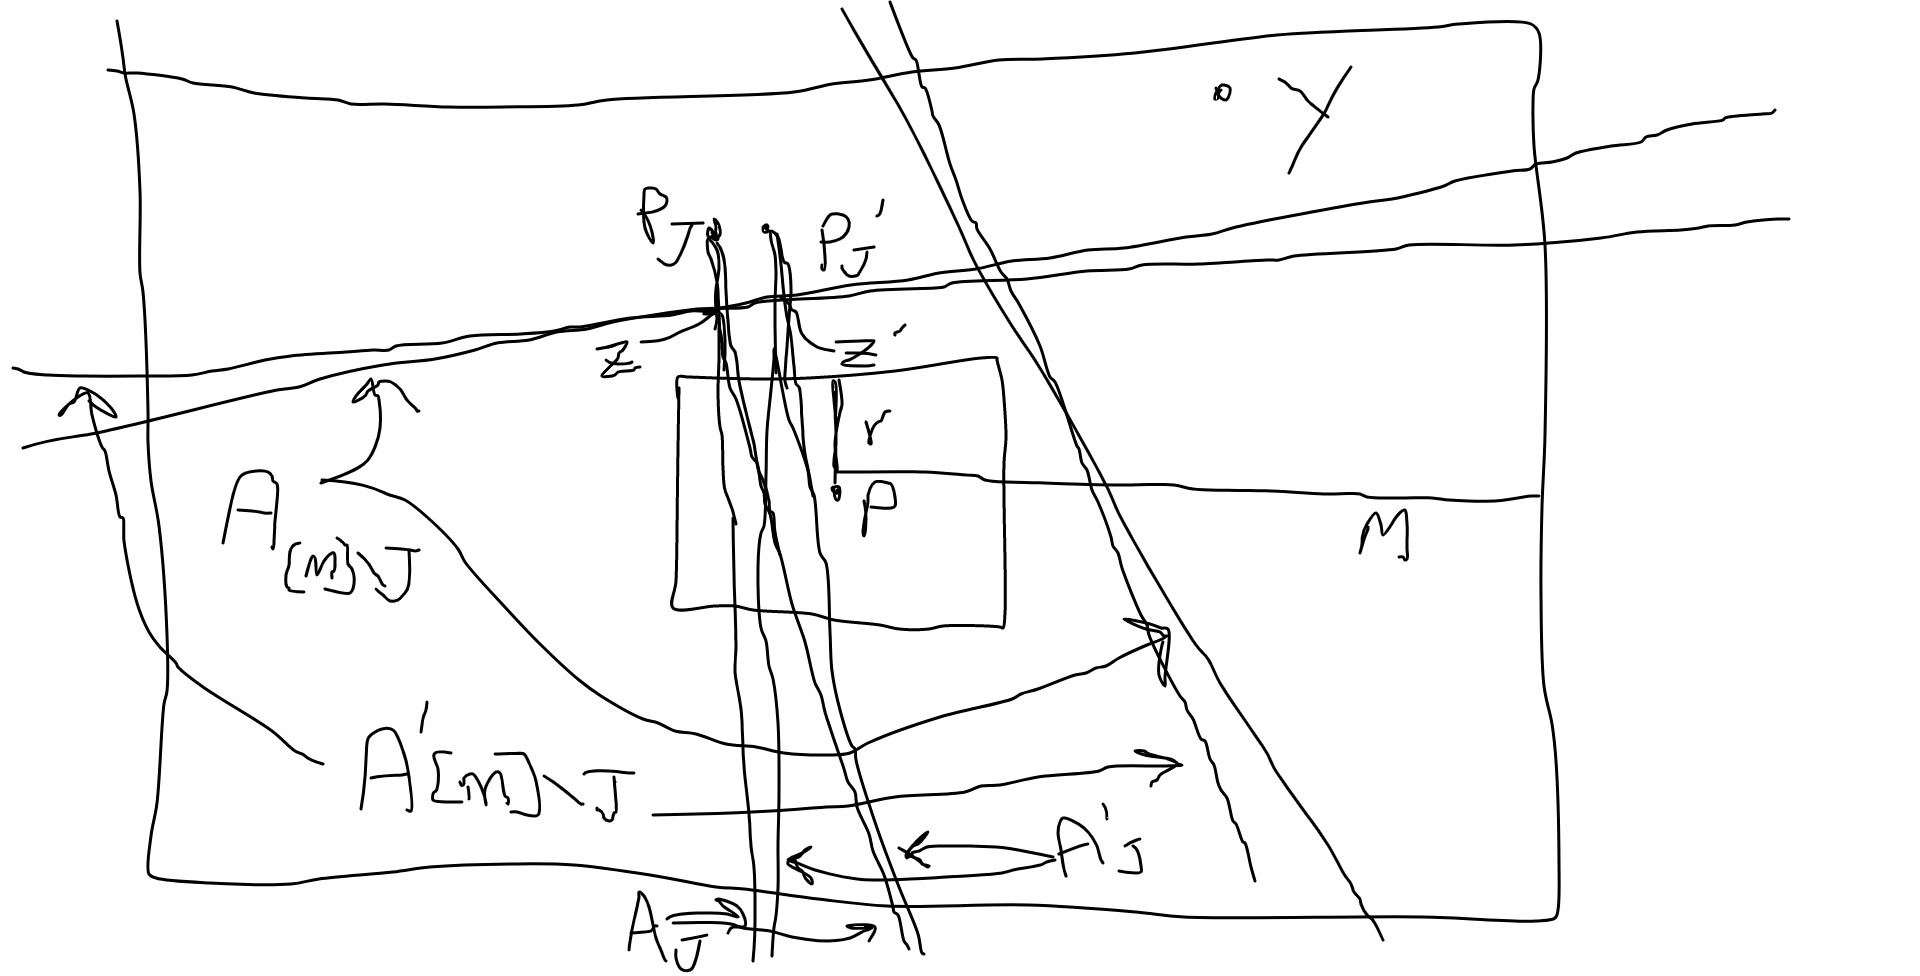
\includegraphics[width=300px]{images/complicated_lemma.png}
    \caption{
    	Here, we bound the distance between the projections of $y$ onto two different polyhedra.
    	The polyhedra are defined by matrices that are arbitrarily close to eachother.
    	The constraints of the polyhedra are split into two different sets, those that intersect a ball of radius $r$ about a point $p$,
    	and those that do not.
    	The left hand side matrix for the constraints that intersect this ball have a bounded hoffman constant.
	}
    \label{complicated_lemma}
\end{figure}
\newpage




\begin{lemma}
Suppose
$A \in \reals^{m \times n}$;
$b \in \Rm$;
$a^{(0)}, a^{(1)}, p, y \in \Rn$;
and $d, \delta, M > 0$
are given such that
$b > 0$,
$A y \ge \delta$, 
$\left(a^{(0)}\right)^T(y - p) \ge \delta \left\|y - p\right\|$,
$\left(a^{(1)}\right)^T(y - p) \ge \delta \left\|y - p\right\|$.

Define
\begin{align*}
z^{(0)}  = \argmin_{\substack{A(x - p)x \le b \\ \left(a^{(0)}\right)^T \left(x - p\right) \le d}} \|p + y - x\|
\quad \textrm{and} \quad
z^{(1)} = \argmin_{\substack{A(x - p) \le b \\ \left(a^{(1)}\right)^T \left(x - p\right) \le d}} \|p + y - x\|.
\end{align*}
Then, 
\begin{align*}
\left\|z - z'\right\| \le \left(\ldots\right) \|a - a'\|.
\end{align*}
\end{lemma}
\begin{proof}
If $y = 0$, then $z^{(1)} = z^{(2)} = p$ and $z^{(1)} - z^{(2)} = 0$.
From here on, we assume $y \ne 0$.

Note that for $i=0,1$:
\begin{align*}
\left(a^{(i)}\right)^T \left(z^{(1-i)} - p\right) - d 
= \left(a^{(i)} - a^{(1-i)}\right)^T\left(z^{(1-i)} - p\right) + \left(a^{(1-i)}\right)^T\left(z^{(1-i)} - p\right) - d \\
\le \left(a^{(i)} - a^{(1-i)}\right)^T\left(z^{(1-i)} - p\right)
\end{align*}
so that
\begin{align*}
\left| \left(a^{(i)}\right)^T \left(z^{(1-i)} - p\right) - d \right| 
\le \left\|a^{(i)} - a^{(1-i)}\right\| \left\|z^{(1-i)} - p\right\| 
\le \left\|a^{(0)} - a^{(1)}\right\| \left\|y\right\|.
\end{align*}
Also, for $i = 0,1$ and any $t \in [0, 1]$, we have
\begin{align*}
\left[(1 - t) a^{(i)} + t a^{(1-i)}\right]^T\left(z^{(i)} - p\right) - d 
= (1 - t) \left[\left(a^{(i)}\right)^T\left(z^{(i)} - p\right) - d\right] + t \left[{\left(a^{(1-i)}\right)}^T\left(z^{(i)} - p\right) - d\right] \\
\le t \left[\left(a^{(1-i)}\right)^T\left(z^{(i)} - p\right) - d\right] 
\le \left\|a^{(0)} - a^{(1)}\right\| \left\|y\right\|.
\end{align*}
Also,
\begin{align*}
\left[(1 - t) a^{(i)} + t a^{(1-i)}\right]^Ty
= (1 - t) \left(a^{(i)}\right)^Ty + t \left(a^{(1-i)}\right)^Ty  
\ge \left(1-t\right) \delta\left\|y\right\| + t \delta\left\|y\right\|
= \delta\left\|y \right\| \\
\Longrightarrow \frac 1 {\left[(1 - t) a^{(i)} + t a^{(1-i)}\right]^Ty} \le \frac {1} {\delta\left\|y\right\|}.
\end{align*}
% = (1 - t) a^Ty + t {a'}^Ty              - \left[(1 - t) a^Tp + t {a'}^Tp \right]\\


% If ${a}^T z' \le d$ and ${a'}^T z \le d$, then once again, $z' - z = 0$.
% Without loss of generality, suppose that ${a'}^T (z - p) > d$.
% Now,
% \begin{align*}
% {a'}^T\left(z - p\right) - d 
% = \left({a'} - a\right)^T\left(z - p\right) + a^T\left(z - p\right) - d \le \left({a'} - a\right)^T\left(z - p\right) \\
% \Longrightarrow \left|{a'}^T\left(z - p\right) - d\right| 
% \le \left\|a' - a\right\| \left\|z - p\right\| 
% \le \left\|a' - a\right\| \left\|y\right\|
% \end{align*}




Thus, by letting $\lambda = \delta^{-1}\left\|a^{(0)} - a^{(1)}\right\|$, we see for $i=0,1$
\begin{align}
\lambda
= \frac{\left\|a^{(0)} - a^{(1)}\right\|\left\|y\right\|}{\delta \|y\|}
\ge \frac{\left[(1 - t) a^{(i)} + t a^{(1-i)}\right]^T\left(z^{(i)} - p\right) - d}{\left[(1 - t) a^{(i)} + t a^{(1-i)}\right]^Ty}  \\
\Longrightarrow \left[(1 - t) a^{(i)} + t a^{(1-i)}\right]^T \left[z^{(i)} - \lambda y - p\right] \le d \label{plhsop_1}.
\end{align}
We can use $(i,t)=(1, 0)$ and $(i,t)=(0, 1)$ in \cref{plhsop_1} to find for $i=0, 1$
\begin{align*}
\left(a^{(i)}\right)^T\left[\left(z^{(1-i)} - \lambda y\right) - p\right].
\end{align*}
By optimality of the projection, for $i=0,1$:
\begin{align}
\label{plhsop_eqn1}
\|p + y - z^{(i)}\| \le \|p + y - \left(z^{(1-i)} - \lambda y\right)\| \le \|p + y - z^{(1-i)}\| +  \lambda\left\|y\right\|.
\end{align}
With a change of variables, $u^{(i)} = p + y - z^{(i)}$ for $i=0,1$ this becomes
\begin{align*}
\|u^{(i)}\| \le \|u^{(1-i)}\| + \lambda\left\|y\right\|.
\end{align*}
If $\left(a^{(i)}\right)^T z^{(1-i)} \le d$ for both $i=0$ and $1$, then $z^{(0)} = z^{(1)}$ so that $z^{(0)} - z^{(1)} = 0$.
Otherwise, without loss of generality, let $\left(a^{(0)}\right)^T z^{(1)} > d$ so that
convexity of the set $\left\{x \in \Rn | A(x - p) \le b, \left(a^{(0)}\right)^T (x-p) \le d\right\}$ implies
\begin{align}
\label{plhsop_eqn2}
(p + y - z')^T z' \le (p + y - z')^Tz.
\end{align}




Also, by the optimality conditions,
\begin{align*}
y^T\left(z^{(i)} - p\right) \ge 0
\end{align*}
so that
\begin{align*}
\left(u^{(0)}\right)^Tu^{(1)} = \left[y - \left(z^{(0)} - p\right)\right]^T\left[y - \left(z^{(1)} - p\right)\right] \\
= \left\|y\right\|^2 - y^T\left(z^{(0)} - p + z^{(1)} - p\right) + \left(z^{(0)} - p\right)^T\left(z^{(1)} - p\right) \\
\ge \left\|y\right\|^2 + \left\|z^{(0)} - p\right\|^T\left\|z^{(1)} - p\right\|
\end{align*}


Suppose that both
\begin{align*}
\left(u^{(0)}\right)^Tu^{(1)} \le \left \| u^{(0)} \right \|^2 			\quad \textrm{and} \quad
\left(u^{(0)}\right)^Tu^{(1)} \le \left \| u^{(1)} \right \|^2.
\end{align*}
\begin{align*}
\left\|u^{(0)} - u^{(1)}\right\|^2 =  \left \| u^{(0)} \right \|^2 + \left \| u^{(1)} \right \|^2 - 2 \left(u^{(0)}\right)^Tu^{(1)}
\end{align*}

Also, $a' z \ge d$ and 


% \begin{align*}
% (p + y - z)^T z' \le (p + y - z)^Tz.
% \end{align*}

With the variables $u = p + y - z$, $u' = p + y - z'$, and $\gamma = \delta^{-1}\left\|a - a'\right\|\left\|y\right\|$, we can summarize \cref{plhsop_eqn1} and \cref{plhsop_eqn2}
with 
\begin{align*}
\|u'\| \le \|u\| + \gamma
\Longrightarrow \|u'\|^2 \le \|u\|^2 + 2\|u\| \gamma + \gamma^2
\end{align*}
and
\begin{align*}
{u'}^Tz' \le {u'}^T z
\Longrightarrow -{u'}^Tz' + {u'}^T\left(p + y\right) 
\ge -{u'}^T z + {u'}^T \left(p + y\right) \\
\Longrightarrow {u'}^T\left(p + y - z'\right) \ge {u'}^T \left(p + y - z\right)
\Longrightarrow {u'}^Tu' \ge {u'}^T u
\Longrightarrow -{u'}^Tu' \le -{u'}^T u.
\end{align*}


\begin{align*}
u^Tu' \le \|u'\|^2 \\
u^T\frac{u'}{\|u'\|} \le \|u'\| \\
u^T\frac{u'}{\|u'\|} \le \|u\| + \gamma \\
\frac{u^T}{\|u\|}\frac{u'}{\|u'\|} \le 1 + \gamma\|u\|^{-1}
\end{align*}


Finally, we can compute
\begin{align*}
\|z - z'\|^2 
= \|u - u'\|^2 
= \|u\|^2 - 2u^Tu' + \|u'\|^2
= \|u\|^2 - 2u^Tu' + \|u'\|^2
\end{align*}


\begin{align*}
\|z - z'\|^2 
= \|z\|^2 - 2 z^Tz' + \|z'\|^2 
\le \|z\|^2 - 2 \|z\|^2 + \|z'\|^2 = \|z'\|^2 - \|z\|^2
\le \delta^2
\end{align*}


\begin{align*}
\\
\\
\\
\\
\\
\end{align*}

and
\begin{align*}
\left\|z - \lambda y - z\right\| = \delta^{-1}\left\|a - a'\right\|\left\|y\right\|.
\end{align*}
Thus,
\begin{align*}
\left\|p + y - z'\right\| \le \left\|p + y - z - \lambda \left(y - p\right)\right\| \le \left\|p + y - z\right\| + \delta^{-1}\left\|a - a'\right\|\left\|y\right\|.
\end{align*}

\begin{comment}
Some more logic here...
\end{comment}

\begin{align*}
\left\|z - z'\right\| \le K \left\|a - a'\right\| \left\|y\right\|
\end{align*}



% Let 
% \begin{align*}
% r  = \left\|p + y - z\right\|
% \quad \textrm{and} \quad
% r' = \left\|p + y - z'\right\|
% \end{align*}
% and without loss of generality, suppose that $r \le r'$.


% 
% 
% Let
% \begin{align*}
% \mathcal P(t) = \left\{
% x \in \Rn \bigg | 
% Ax \le b, 
% \left[(1 - t) a + t a'\right]^T (x - p) \le d
% \right\}
% \end{align*}
% so that
% \begin{align*}
% z = P_{\mathcal P(0)}(p + y) \\
% z' = P_{\mathcal P(1)}(p + y) \\
% \end{align*}
% 
% \begin{align*}
% v(t) = P_{\mathcal P(t)}(p + y) \\
% z(t) = \frac 1 2 \left\| z - v(t)\right\|^2 \\
% \end{align*}
% 
% For any particular $t_0 \in [0, 1]$, there exists $\mu \in \mathbb R_{\ge 0}$ and $\lambda \in \mathbb R^m_{\ge 0}$ such that
% \begin{align*}
% p + y - v(t_0) = \mu \left[(1 - t_0) a + t_0 a'\right]^T + A^T\lambda
% \end{align*}
% 
% \begin{align*}
% z'(t) = 2 \nabla v(t)^T\left( z - v(t)\right) \\
% \nabla v(t) = 
% \end{align*}
% 
% Let $\mathcal I(t)$ be the set of active indices:
% \begin{align*}
% \mathcal I (t) = \left\{i \in [m] \bigg | A_i v(t) = b_i \right\}
% \end{align*}
% 
% For some sufficiently small $h \in \reals$, we will have 
% \begin{align*}
% v(t+h) = 
% \end{align*}
% 
\end{proof}









\begin{lemma}
Suppose that 
\begin{align*}
\|z \|^2 \le \|z'\|^2 \le \|z \|^2 + \delta^2 \\
\|z\|^2 \le {z}^Tz'
\end{align*}
then
\begin{align*}
\|z - z'\| \le ?
\end{align*}
\end{lemma}
\begin{proof}
\begin{align*}
\|z - z'\|^2 
= \|z\|^2 - 2 z^Tz' + \|z'\|^2 
\le \|z\|^2 - 2 \|z\|^2 + \|z'\|^2 = \|z'\|^2 - \|z\|^2
\le \delta^2 \\
\Longrightarrow \|z - z'\| \le \delta
\end{align*}
\end{proof}









% 
% 
% \begin{lemma}
% Suppose
% $A \in \reals^{m \times n}$;
% $b \in \Rm$;
% $a, a', p \in \Rn$;
% and $d \in \reals$
% are given such that
% $Ap < b$ and $d > 0$.
% Define
% \begin{align*}
% z  = \argmin_{\substack{Ax \le b \\ a^T \left(x - p\right) \le d}} \|p + y - x\|
% \quad \textrm{and} \quad
% z' = \argmin_{\substack{Ax \le b \\ {a'}^T \left(x - p\right) \le d}} \|p + y - x\|.
% \end{align*}
% \end{lemma}
% \begin{proof}
% If both $a^T\left(z' - p\right) \le d$ and ${a'}^T \left(z - p\right) \le d$, then we have $z - z' = 0$.
% Without loss of generality, assume that 
% $a^T\left(z' - p\right) > d \Longrightarrow a^T\left(z' - p\right) - d > 0$.
% By the contraction property of projections
% \begin{align*}
% \left\|z' - p\right\|
% \le \left\|P_{\{x | Ax \le b, {a'}^T(x-p) \le d\}}\left(p + y\right) - P_{\{x | Ax \le b, {a'}^T(x-p) \le d\}}\left(p\right)\right\|
% \le \left\|p + y - p\right\|
% = \|y\|.
% \end{align*}
% Combine this with ${a'}^T \left(z' - p\right) \le d \Longrightarrow {a'}^T \left(z' - p\right) - d \le 0$ to find
% \begin{align*}
% a^T\left(z' - p\right) - d 
% = a^T\left(z' - p\right) - {a'}^T \left(z' - p\right) + {a'}^T \left(z' - p\right) - d 
% \le \left(a - a'\right)^T \left(z' - p\right) \\
% \le \left\|a - a'\right\| \left\|z' - p\right\|
% \le \left\|a - a'\right\| \|y\|.
% \end{align*}
% We can compute
% \begin{align*}
% a^T\left(\frac{d + a^Tp}{a^Tz'}z' - p\right) = d + a^Tp - a^Tp = d
% \end{align*}
% and
% \begin{align*}
% \left\|z' - \frac{d + a^Tp}{a^Tz'}z'\right\| 
% = \left\|z'\right\|\left|\frac{a^Tz'}{a^Tz'} - \frac{d + a^Tp}{a^Tz'}\right|
% \le \left\|z'\right\| \frac{\left\|y\right\|}{a^Tz} \left\|a - a'\right\|
% \end{align*}
% 
% 
% 
% 
% 
% 
% 
% 
% 
% 
% Let $s = \frac{a^Tz' - d}{a^T\left(z' - p\right)}$.
% Notice that
% $s a^T\left(p - z'\right) = d - a^Tz' \Longrightarrow  a^T\left[z' + s \left(p - z'\right)  \right] = d $
% and
% $\left\|z' - s\left(p - z'\right) - z'\right\| 
% = \frac{a^Tz' - d}{a^T\left(z' - p\right)}\left\| z' - p\right\| 
% \le \frac{\left\|z' - p\right\|}{a^T\left(z' - p\right)} \|a - a'\| \|z'\|$
% \end{proof}








\begin{lemma}
\label{master_projection_lemma}
Let $\atr$ and $\btr$ be defined by \cref{define_atr}.
Let $H(A)$ be defined by \cref{hoffman_theorem}.

Let $A, A'$ be $m \times n$ matrices;
$p, y \in \Rn$; $b, b' \in \Rm$;
and $M,\delta, r, \epsilon > 0$ be given 
such that 
with the definition
\begin{align*}
J = \left\{i \in [m] \; \bigg | \; b_i \le \|A_i\|r  \right\}
\end{align*}
all the following identities are satisfied:
\begin{align*}
Ap \le b,
\quad 
A'p \le b', \\
\left\|A_i - A'_i \right\| \le \epsilon\quad \forall i \in [m],
\quad 
\left|b_i - b'_i \right| \le \epsilon \quad \forall i \in [m], \\
\delta \le \left\|A_i\right\| \le M \quad \forall i \in [m],
\quad 
\delta \le \left\|A'_i\right\| \le M \quad \forall i \in [m], \\
\left|b_i\right| \le M \quad \forall i \in [m],
\quad 
\left|b'_i\right| \le M \quad \forall i \in [m], \\
H\left(A_J\right) \le M, \quad H\left(A'_J\right) \le M.
\end{align*}
Then
\begin{align*}
\|z - z'\| \le \left(\ldots\right) \epsilon
\end{align*}
where
\begin{align*}
z  = \argmin_{x \in \Rn | A (x - p) \le b }\left\|p + y - x\right\|
\quad \textrm{and} \quad
z' = \argmin_{x \in \Rn | A'(x - p) \le b'}\left\|p + y - x\right\|.
\end{align*}
\end{lemma}
\begin{proof}



Because $H\left(A_J\right) \le M$, we have that if 
$\mathcal A = \left\{i \in J | A_i\left(y - p\right) \ge 0 \right\}$, and
$\mathcal A' = \left\{i \in J | A'_i\left(y - p\right) \ge 0 \right\}$, then
\begin{align*}
M \ge H(A_J) 
= \max_{\mathcal J \in \mathcal S_h(A_J)} \left[\min_{v \in R^{\mathcal J}_+, \|v\| = 1}  \left\|A_{\mathcal J}^Tv\right\| \right]^{-1}
\ge \left[\min_{v \in R^{\mathcal A}_+, \|v\| = 1}  \left\|A_{\mathcal A}^Tv\right\| \right]^{-1}
\ge \frac{\left\|y - p\right\|}{\left\|A_{\mathcal A}^T (y - p) \right\|} \\
\Longrightarrow A_{\mathcal A}^T (y - p)  \ge \frac 1 M \left\|y - p\right\|.
\end{align*}
Also, if $i \in [m] \setminus J$ and $A_i(y - p) \ge b_i$, then
\begin{align*}
A_i \left(y - p\right) \ge b_i - A_ip + A_ip \ge \|A_i\| r + A_ip
\end{align*}


\begin{align*}
\| y - p \| \le \|y\| + \|p\| \\
\frac 1{\| y - p \|} \ge \frac 1 {\|y\| + \|p\|} \\
\end{align*}



\begin{align*}
A_i \left(y - p\right) \ge A_i y + r \|A_i\| - b_i 
\end{align*}



\begin{align*}
\|A_i\| r + A_ip \ge \|A_i\| \left\|y - p\right\| \\
r + \frac{A_i}{\|A_i\|}p \ge  \left\|y - p\right\| \\
\end{align*}

% 
% 
% \begin{align*}
% b_i - A_ip > \|A_i\| r 
% \Longrightarrow - A_ip > \|A_i\|r - b_i
% \Longrightarrow A_i\left(p_J - p\right) > \|A_i\|r \ge \delta r > 0 \\
% \Longrightarrow \frac{1}{A_i\left(p_J - p\right)} < \frac{1}{\delta r} < \frac 2 {\delta r}.
% \end{align*}


\begin{align*}
b_i \le \|A_i\| r \\
A_i \left(p + t \frac {A_i^T} {\|A_i\|} \right) = b_i \\
A_i p + t \frac {A_i A_i^T} {\|A_i\|} = b_i \\
A_i p + t \|A_i\| = b_i \\
t \|A_i\| = b_i - A_i p\\
t = \frac{b_i - A_i p}{\|A_i\|} \ge r \\
b_i - A_i p \ge r\|A_i\| \\
\end{align*}

\end{proof}




% % Define
% % \begin{align*}
% % K = M\|y - p\| + \max\left\{
% % \max_{i \in [m]}\left\{A_ip - b_i\right\},
% % \max_{i \in [m]}\left\{A'_ip - b'_i\right\},
% % \right\}
% % \end{align*}
% 
% Note that
% \begin{align*}
% |A_ip_J - b_i| \le M(M+1) \\
% |A'_ip'_J - b'_i| \le M(M+1) \\
% \bigg|
% |A_ip_J - b_i| - |A'_ip'_J - b'_i|
% \bigg| \le |
% A_ip_J - b_i - A'_ip'_J + b'_i
% | \\
% \le |A_ip_J - A_i p'_J| + |A_ip'_J - A'_ip'_J| + |b'_i - b_i|
% \le M\epsilon + M\epsilon + \epsilon = \epsilon (2M + 1).
% \end{align*}
% 
% 
% 
% Let 
% \begin{align*}
% v(t) = p_J + t(p - p_J)
% \quad
% v'(t) = p'_J + t(p - p'_J).
% \end{align*}
% Let $i \in [m] \setminus J$.
% If $A_ip_J > b_i$, then 
% \begin{align*}
% b_i - A_ip \le \|A_i\| r 
% \Longrightarrow - A_ip > \|A_i\|r - b_i
% \Longrightarrow A_i\left(p_J - p\right) > \|A_i\|r \ge \delta r > 0 \\
% \Longrightarrow \frac{1}{A_i\left(p_J - p\right)} < \frac{1}{\delta r} < \frac 2 {\delta r}.
% \end{align*}
% If $s_i = \frac{A_ip_J - b_i}{A_i(p_J - p)}$, we have
% \begin{align*}
% t \ge s_i
% \Longrightarrow tA_i(p - p_J) \le b_i - A_ip_J 
% \Longrightarrow A_iv(t) \le b_i
% \end{align*}
% and
% \begin{align*}
% \left\|p_J - v\left(s_i\right)\right\|
% = \frac{\left(A_ip_J - b_i\right)\left\|p - p_J\right\|}{A_i(p_J - p)}
% < 2\frac{\left(A_ip_J - b_i\right)\left\|p - p_J\right\|}{\delta r}
% \le \frac{2K}{\delta r}\left\|p - p_J\right\|.
% \end{align*}
% 
% 
% Likewise, if $A'_ip'_J > b'_i$, then 
% \begin{align*}
% - A_ip > \|A_i\|r - b_i
% \Longrightarrow \epsilon\|p\| - A'_i p \ge \left(\|A'_i\| - \epsilon\right)r - b'_i - \epsilon \\
% \Longrightarrow -A'_ip > \|A'_i\|r - b'_i - \epsilon\left(1 + \|p\| + r\right) \\
% \Longrightarrow A'_i\left(p'_J - p\right) > \delta r - \frac 1 2 \delta r = \frac 1 2 \delta r > 0 \\
% \Longrightarrow \frac{1}{A'_i\left(p'_J - p\right)} < \frac{2}{\delta r}.
% \end{align*}
% If $s'_i = \frac{A'_ip'_J - b'_i}{A'_i(p'_J - p)}$, we have
% \begin{align*}
% t \ge s'_i
% \Longrightarrow tA'_i(p - p'_J) \le b'_i - A'_ip'_J 
% \Longrightarrow A'_iv(t) \le b'_i
% \end{align*}
% and
% \begin{align*}
% \left\|p'_J - v'\left(s'_i\right)\right\|
% = \frac{\left(A'_ip'_J - b'_i\right)\left\|p - p'_J\right\|}{A'_i(p'_J - p)}
% < 2\frac{\left(A'_ip'_J - b'_i\right)\left\|p - p'_J\right\|}{\delta r}
% \le \frac{2K}{\delta r}\left\|p - p'_J\right\|
% \end{align*}
% 
% Consider any $i \in [m] \setminus J$,
% and let
% \begin{align*}
% \gamma_1 = \frac{A_ip_J - b_i}{A_i(p_J - p)}
% \quad \textrm{and} \quad
% \gamma_2 = \frac{A'_ip'_J - b'_i}{A'_i(p'_J - p)}.
% \end{align*}
% 
% 
% \paragraph{Case 1}
% Suppose that both $A_ip_J > b_i$ and $A'_ip'_J > b'_i$.
% 
% Then
% \begin{align*}
% \gamma_1 - \gamma_2
% \end{align*}
% 
% 
% Notice that
% \begin{align*}
% \epsilon 
% \ge \left\|p_J - p'_J\right\|
% = \left\|p_J - p + \left(p - p'_J\right)\right\|
% \ge \bigg|
% \left\|p - p_J\right\| - \left\|p - p'_J\right\|
% \bigg| \\
% p_J - v(s_i) = p_J - p_J - s_i \left(p - p_J\right) \\
% p'_J - v'(s_i) = p'_J - p'_J - s'_i \left(p - p_J\right)
% \end{align*}
% implies
% \begin{align*}
% \bigg||s_i| - |s'_i|\bigg| =
% \bigg|
% \left\|p_J - v\left(s_i\right)\right\| -
% \left\|p'_J - v'\left(s'_i\right)\right\|
% \bigg| \le \frac{2K}{\delta r} \epsilon
% \end{align*}
% so that with
% we have
% \begin{align*}
% v\left(s_i\right) - v'\left(s'_i\right) 
% = \left(p_J - p'_J\right) + \left(p'_J - v(s'_i)\right) - \left(p_J - v(s_i)\right) \\
% = \left(p_J - p'_J\right) 
% + \gamma_2 \left(p - p'_J\right)
% - \gamma_1 \left(p - p _J\right) \\
% = \left(p_J - p'_J\right) 
% + \left(\gamma_2 - \gamma_1\right) p
% + \gamma_1 p _J - \gamma_1 p'_J
% + \gamma_1 p'_J - \gamma_2 p'_J \\
% \Longrightarrow \left\|v\left(s_i\right) - v'\left(s'_i\right) \right\|
% \le \left(1 + \gamma_1 \right)\left\|p_J - p'_J\right\| + \left(\|p\| + \|p'_J\|\right)\left|\gamma_1 - \gamma_2\right|
% \end{align*}
% 
% \begin{align*}
% \gamma_1 p_J - \gamma_2 p'_J
% \end{align*}
% 
% 
% % \begin{align*}
% % v\left(s_i\right) - v'\left(s'_i\right) 
% % = p_J + s_i\left(p - p_J\right) - p'_J - s'_i\left(p - p'_J\right) \\
% % = p + \left(1 - s_i\right)\left(p_J - p\right) - p - \left(1 - s'_i\right)\left(p'_J - p\right) \\
% % = \left(1 - s_i\right)\left(p_J - p\right) - \left(1 - s'_i\right)\left(p'_J - p\right) \\
% % = \left(p_J - p'_J\right) - s_i\left(p_J - p\right) + s'_i\left(p'_J - p\right) \\
% % = \left(p_J - p'_J\right) + \left(p_J - v(s_i)\right) - \left(p'_J - v(s'_i)\right)
% % \end{align*}
% 
% % = p_J + s_i\left(p - p_J\right) - p'_J - s'_i\left(p - p'_J\right) \\
% % = p + \left(1 - s_i\right)\left(p_J - p\right) - p - \left(1 - s'_i\right)\left(p'_J - p\right) \\
% % = \left(1 - s_i\right)\left(p_J - p\right) - \left(1 - s'_i\right)\left(p'_J - p\right) \\
% % = \left(p_J - p'_J\right) - s_i\left(p_J - p\right) + s'_i\left(p'_J - p\right) \\
% 
% 
% 
% 
% 
% % \begin{align*}
% % \left\|v\left(s_i\right) - v'\left(s'_i\right)\right\|
% % = \left\|p_J + s_i\left(p - p_J\right) - p'_J - s'_i\left(p - p'_J\right)\right\| \\
% % = \left\|p + \left(1 - s_i\right)\left(p_J - p\right) - p - \left(1 - s'_i\right)\left(p'_J - p\right)\right\| \\
% % \le \left\|p\right\|\left|s'_i - s_i\right| + \left\|p_J - p'_J\right\| + \left\|s_ip_J - s'_i p_J\right\| + \left\|s'_ip_J - s'_ip'_J\right\| \\
% % \le \left(\|p_J\| + \left\|p\right\|\right)\left|s'_i - s_i\right| + \left(1 + |s'_i|\right)\left\|p_J - p'_J\right\|
% % \end{align*}
% 
% 
% 
% 
% 
% 
% 
% \paragraph{Case 2}
% Suppose that both $A_ip_J > b_i$ and $A'_ip'_J \le b'_i$.
% Then 
% \begin{align*}
% \bigg|
% |A_ip_J - b_i| - |A'_ip'_J - b'_i|
% \bigg| 
% \le \epsilon (2M + 1).
% \end{align*}
% \paragraph{Case 3}
% Suppose that both $A_ip_J \le b_i$ and $A'_ip'_J > b'_i$.
% 
% \paragraph{Case 4}
% Suppose that both $A_ip_J \le b_i$ and $A'_ip'_J \le b'_i$.
% Then
% \begin{align*}
% \left\|v\left(s_i\right) - v'\left(s'_i\right)\right\| 
% = \left\|p_J - p'_J\right\| \le \epsilon.
% \end{align*}
% 
% Let $u = p_J$ if $A_ip_J \le b_i \forall i \in [m] \setminus J$ and $u' = p'_J$ if $A'_ip'_J \le b'_i \forall i \in [m] \setminus J$.
% Otherwise, let
% \begin{align*}
% j = \argmax_{\substack{
% i \in [m] \setminus J \\
% A_ip_J > b_i
% }}\{s_i\},
% \quad u = v\left(s_j\right),
% \quad 
% j' = \argmax_{\substack{
% i \in [m] \setminus J \\
% A'_ip'_J > b'_i
% }}\{s'_i\},
% \quad \textrm{and} \quad
% u' = v'\left(s'_{j'}\right).
% \end{align*}
% Then, both $Au \le b$ and
% $A'u' \le b'$.
% 
% \paragraph{Case 1}
% Suppose that for each $i \in [m] \setminus J$, we have both $A_ip_J \le b_i$ and $A'_ip'_J \le b'_i$.
% Then $\|u - u'\| = \|p_J - p'_J\| \le \epsilon$.
% 
% \paragraph{Case 2}
% Suppose that 
% 
% 
% 
% Suppose that 
% Suppose that for each $i \in [m] \setminus J$, we have both $A_ip_J \le b_i$ and $A'_ip'_J \le b'_i$.
% Then $\|u - u'\| = \|p_J - p'_J\| \le \epsilon$.
% 
% 
% and
% \begin{align*}
% \epsilon\left(M + \left\|p'_J\right\| + 1\right)
% \ge \left|A_ip_J - A_i p'_J\right| + \left|A_i p'_J- A'_ip'_J\right| + \left| b_i + b'_i\right| \\
% \ge \left|A_ip_J - A'_ip'_J - b_i + b'_i\right|
% \ge \bigg|
% \left|A_ip_J - b_i\right| - \left|A'_ip'_J - b'_i\right|
% \bigg|
% \end{align*}
% imply
% \begin{align*}
% \bigg|
% \left(\left|A_ip_J - b_i\right| - \left|A'_ip'_J - b'_i\right|\right)
% \left(\left\|p - p_J\right\| - \left\|p - p'_J\right\|\right)
% \bigg|
% \end{align*}
% 
% 
% 
% 
% If $|x - x'| \le \epsilon$ and $|y - y'| \le \delta$, then
% \begin{align*}
% x - \epsilon \le x' \le x + \epsilon \\
% y - \delta \le y' \le y + \delta \\
% \end{align*}
% 
% \begin{align*}
% |xy - x'y'| 
% = |xy - xy' + xy' - x'y'| 
% = |x(y - y') + y'(x - x')| 
% \le |x||y - y'| + |y'||x - x'|
% \le \delta |x| + \epsilon|y'|
% \end{align*}
% 
% 
% 
% \begin{align*}
% \|x + t_1(p - x) - y - t_2(p - y)\|  \\
% \le |t_1 - t_2| \|p\| + \|x - y\| + \|t_1x - t_2 y\| \\
% \le |t_1 - t_2| \|p\| + \|x - y\| + \|t_1x - t_2 x\| + \|t_2 x - t_2 y\| \\
% \le |t_1 - t_2| \|p\| + \|x - y\| + \|x\| \|t_1 - t_2\| + |t_2| \|x - y\| \\
% \end{align*}
% % \le |t_1 - t_2| \|p\| + \|x - y\| + \|t_1x - t_1y + t_1y - t_2 y\|
% % \le \|x(1 - t_1) - y(1 - t_2) + t_1p - t_2p)\| 
% 
% 
% 
% \begin{align*}
% \left\|v\left(s_i\right) - v'\left(s'_i\right)\right\|
% \le \|p_J - p'_J\| + \left\|\left(p_J - v\left(s_i\right)\right) - \left(p'_J - v'\left(s'_i\right)\right)\right\|
% \end{align*}
% 
% 
% 
% \begin{align*}
% \left\|v\left(s_i\right) - v'\left(s'_i\right)\right\|
% \le \left\|p_J + s_i \left(p - p_J\right) -p'_J - s'_i \left(p - p'_J\right)\right\| \\
% \le \left\|p_J + s_i \left(p - p_J\right) -p'_J - s'_i \left(p - p'_J\right)\right\|
% \end{align*}
% 
% 
% \begin{align*}
% \|x + t_1(p - x) - y - t_2(p - y)\|  \\
% \le |t_1 - t_2| \|p\| + \|x - y\| + \|t_1x - t_2 y\| \\
% \le |t_1 - t_2| \|p\| + \|x - y\| + \|t_1x - t_2 x\| + \|t_2 x - t_2 y\| \\
% \le |t_1 - t_2| \|p\| + \|x - y\| + \|x\| \|t_1 - t_2\| + |t_2| \|x - y\| \\
% \end{align*}
% 
% 
% 
% \begin{align*}
% \|t_1(p - x) - t_2(p - y)\| \le \|t_1(p - x) - t_1(p-y)\| + \|t_1(p-y) - t_2(p - y)\| \\
% \le |t_1|\|p - x - p + y\| + \left|t_1 - t_2\right|\left\|p - y\right\|
% \end{align*}

% \le \left\|p\right\|\left|s'_i - s_i\right| + \left\|p_J - p'_J\right\| + \left\|s_ip_J - s'_ip'_J\right\| \\


% 
% \begin{align*}
% \left\|x\right\| \frac{y}{\left\|y\right\|}
% \end{align*}
% 
% \begin{align*}
% \left\|y\right\| - \left\|x \right\| \le \left\|y - x\right\| \\
% 1 - \frac{\left\|x \right\|}{\left\|y\right\|} \le \frac{\left\|y - x\right\|}{\left\|y\right\|} \\
% \end{align*}
% 
% 
% \begin{align*}
% \left\|x -  \frac{\left\|x\right\|}{\left\|y\right\|} y\right\|
% \le \left\|x - \frac{\left\|x\right\|}{\left\|y\right\|} x \right\|+ \left\|\frac{\left\|x\right\|}{\left\|y\right\|} x - \frac{\left\|x\right\|}{\left\|y\right\|} y\right\|
% = \left\|x\right\|\left(1 - \frac{\left\|x\right\|}{\left\|y\right\|}\right) + \frac{\left\|x\right\|}{\left\|y\right\|} \left\| x - y\right\| \\
% \le \left\|x\right\|\frac{\left\|y - x\right\|}{\left\|y\right\|} + \frac{\left\|x\right\|}{\left\|y\right\|} \left\| x - y\right\| \\
% \le 2 \frac{\left\|x\right\|}{\left\|y\right\|} \left\|x - y\right\|
% \end{align*}
% 
% \begin{align*}
% \left|\left\|x\right\| - \left\|y\right\|\right|\le \left\|x - y \right\| \le a \left\|y\right\| \\
% \left|\frac{\left\|x\right\|}{\left\|y\right\|} - 1\right|\le \left\|x - y \right\| \le a 
% \end{align*}
% 
% \begin{align*}
% \left\|s x - s' y\right\|
% \le \left\|x - y\right\| + 
% \end{align*}
% 
% \begin{align*}
% \left\|s x - s' y\right\| 
% \le \left\|s x -  s \frac{\left\|x\right\|}{\left\|y\right\|} y\right\| + \left\| s \frac{\left\|x\right\|}{\left\|y\right\|} y - s' y \right\|
% \end{align*}
% \begin{align*}
% \left\|s x - s' y\right\| 
% \le \left\|s x -  s y\right\| + \left\| s y - s' y \right\|
% \le s \left\|x - y\right\| + \left|s - s'\right| \left\| y \right\|
% \end{align*}
% 
% \begin{align*}
% \left\|p_J - \right\| \frac{p'_J - p}{\left\|p'_J - p\right\|} 
% \end{align*}






\begin{lemma}
Suppose
$A \in \reals^{m \times n}$;
$b \in \Rm$;
$a, p, y \in \Rn$;
and $d, d', \delta, M > 0$
are given such that
$\|y\| \le M$, $Ap < b$, $A (y - p) \ge \delta$, $a^T(y - p) \ge \delta \left\|y - p\right\|$, ${a'}^T(y - p) \ge \delta \left\|y - p\right\|$.

Define
\begin{align*}
z  = \argmin_{\substack{Ax \le b \\ a^T \left(x - p\right) \le d}} \|p + y - x\|
\quad \textrm{and} \quad
z' = \argmin_{\substack{Ax \le b \\ {a}^T \left(x - p\right) \le d'}} \|p + y - x\|.
\end{align*}
Then, 
\begin{align*}
\left\|z - z'\right\| \le \left(\ldots\right) |d - d'|.
\end{align*}
\end{lemma}
\begin{proof}
\begin{comment}
More logic here...
\end{comment}
\end{proof}




% First, we will state some well known theorems without proof.

\subsection{From Huffman}




\color{red}
\begin{align*}
\min_{v \in \Rm_+, \|v\| = 1} \left\|A^Tv\right\| 
\ge \phi \left[\min_{v \in \Rm_+, \|v\| = 1} \left\|A^Tv\right\|_{\infty}\right] 
=   \phi \left[\min_{v \in \Rm_+, \|v\| = 1} \max_{i \in \activeconstraintsk} \left|\gmcik^T v\right|\right]
\end{align*}



There exists an $N \in \naturals$ such that if $k, l \ge N$, we have $\left\|\nabla \mcik\left(\xk\right) - \nabla \mcil\left(\xl\right) \right\| \le \epsilon$.

\begin{align*}
\min_{v \in \Rm_+, \|v\| = 1} \max_{i \in \activeconstraintsk} \left|\gmcik^T v\right|
\end{align*}


By definition \cref{define_u},
\begin{align*}
\huk \in -\argmin_{\|u\| = 1} \max_{i \in \activeconstraintsk} u^T \frac{\gmcik}{\left\|\gmcik\right\|}
\end{align*}
By \cref{define_thetamink},
\begin{align*}
\thetamink = \min_{i \in \activeconstraintsk} \left(-\hgik\right)^T \huk.
\end{align*}



\begin{align*}
\frac 1 {}
\end{align*}
\color{black}



\color{red}
\begin{theorem}[Hoffman's theorem of \cite{hoffman_theorem}]
\label{hoffman_old}
Suppose that the system $Ax \le b$ is consistent and $A$ is normalized so that $\sum_{i = 0}^n{A}_{i,j}^2 = 1$ for all $1 \le j \le m$.
Then there exists a value $\huff(A) > 0$ such that for any such $x$, there exists an $x_0$ with
\begin{align*}
Ax_0 \le b \\
\|x - x_0\|_{\infty} \le \phi_{\infty, 2}\|x - x_0\|_2 \le {\huff(A)} \|(Ax - b)^+\|_\infty.
\end{align*}

This $\huff(A,b)$ is defined as follows, where $i_1, i_2, \ldots, i_r$ are the linearly independent rows of $A$ and $C_{i,j}$ is the $i,j$ cofactor of $C$:
\begin{align*}
\Lambda(C) = \sqrt{\sum_{j=1}^r\bigg(\sum_{i=1}^r C_{i,j}\bigg)^2}, \quad
{\huff(A)} \le \phi_{\infty, 2}\sqrt{\frac{\sum_{1 < j_1 < \ldots < j_k \le n} \|\Lambda^{j_1,\ldots,j_r}_{i_1,\ldots, i_r}\|_{\infty}^2}{\sum_{1 < j_1 < \ldots < j_k \le n} \|A^{j_1,\ldots,j_r}_{i_1,\ldots, i_r}\|_{\infty}^2}}.
\end{align*}
\end{theorem}



\begin{theorem}[Equation 1 and 2 of \cite{pena2018algorithm}]
\label{hoffman}
Let $A \in \mathbb R^{m \times n}$ be given.
Then there is a constant $\huff(A) > 0$ such that for any $b \in \Rm$ with the system $Ax \le b$ consistent and any $x \in \Rn$ we have
\begin{align*}
\|x - x_0\|_{\infty} \le \huff(A) \|(Ax - b)^+\|_\infty.
\end{align*}
where
\begin{align*}
\begin{array}{ccc}
x_0 = & \argmin_{y \in \Rn} & \|x - y\| \\
      & \textrm{s.t.}    & Ay \le b
\end{array}
\end{align*}
This constant can be computed as
\begin{align*}
\huff(A) = \max_{J \subseteq \{1,\ldots,m\}, \textrm{rank}(A_J) = J} \frac 1 {\min_{v \in R^J_{+}, \|v\| = 1} \|A_J^Tv\|}
\end{align*}
Here, $A_J \in \mathbb R^{J \times n}$ is the submatrix of $A$ formed from the rows in $J$, and $\textrm{rank}(A)$ is the row rank of $A$.
\end{theorem}

\color{black}


% \begin{lemma}[Theorem 1.1 of \cite{continuity_of_inverse}]
% \label{inverse_is_continuous}
% For two matrices $A$ and $B$, if $B = A + E$ and $\text{rank}(A) = \text{rank}(B)$, then
% 
% \begin{align*}
% \|B^{\dagger} - A^{\dagger} \|_\infty \le \frac{1 + \sqrt{5}}{2} \|A^{\dagger}\|_\infty\|B^{\dagger}\|_\infty\|E\|_\infty.
% \end{align*}
% \end{lemma}




\subsection{From Applying it}


\subsubsection{Applying it}
\color{red}
We will define the following for the next several proofs, using definitions in \cref{mingradassumption} and \cref{bounded_gradients_lemma}:
\begin{align}
\minactivegrad = \min\left\{\mingrad, \frac {\mingradepsilon} {2 \maxgrad}  \right\} \label{define_minactivegrad_orig} \\
\minactivegraddelta = \frac 1 2 \mingradepsilon \label{define_minactivedelta_orig} \\
p^{(k \to l)} = \argmin_{p \in \mathcal F^{(l)}} \|\xk - \gk - p\|^2 \label{bp_define_plk_orig} \\
\mathcal A^{(l \to k)} = \{i \in [m] | c_i(\xk) + \gmcik^T(p^{(l\to k)} - \xk) = 0 \} \label{bp_define_activep} \\
\mathcal F_x = \{ y \in \Rn | c_i(x) + \nabla c_i(x)^T(y - x) \le 0 \quad \forall i \in [m]\}, \label{bp_define_true_linearization} \\
p_x = \argmin_{p \in \mathcal F_x} \|x - \gradf(x) - p\|^2, \label{bp_define_true_projection} \\
\mathcal A_x = \left\{i \in [m] | \left|c_i(x) + \nabla c_i(x)^T(p_x - x)\right| \le \minactivegraddelta \right\}, \label{define_projection_active} \\
p^{(k)} = \argmin_{p \in \feasiblek} \left\| \xk - \nabla f\left(\xk\right) - p \right\|, \label{bp_define_pl} \\
\mathcal A^{(k)} = \left\{i \in [m] | c_i(x) + \gmcik^T\left(p^{(k)} - \xk\right) = 0 \right\}. \label{bp_define_yet_another_thing}
\end{align}
That is, $p^{(l, k)}$ is the projection of $\xk - \gk$ onto iterate $l$'s constraint's linearization,
and $\mathcal A^{(l, k)}$ are the constraints which are active at this projection.

Also, for any iterate $k$ and any $S \subseteq \activeconstraintsk$,
define the $|S|\times n$ matrix $A^k_m(S)$ and vector $b^k_m(S) \in \mathbb R^{|S|}$ 
to be the normalized, linearized constraints corresponding to $S$.
That is, row $j$ of $A^k_m(S)$ is $\frac{\gmcik}{\left\|\gmcik\right\|}$ for some $i \in S\subseteq \activeconstraintsk$, 
and $\left(b^k_m(S)\right)_j = \frac{-c_i(\xk)}{\left\|\gmcik\right\|}$. 
This means that for any $x \in \Rn$,
\begin{align}
\gmcik^T x \le -c_i(\xk) \quad \forall i \in S \Longleftrightarrow A^k_m(S) x \le b^k_m(S), \quad \textrm{and} \quad \left\|\left(A^k_m(S)\right)_i\right\| = 1 \quad \forall i \in S.
\label{define_normalized_model_constraints}
\end{align}
Similarily, define $A^k_c(S)$ and $b^k_c(S)$ so that 
\begin{align}
\nabla c_i\left(\xk\right)^T x \le -c_i(\xk) \quad \forall i \in S \Longleftrightarrow A^k_c(S) x \le b^k_c(S), \quad \textrm{and} \quad \left\|\left(A^k_c(S)\right)_i\right\| = 1 \quad \forall i \in S.
\label{define_normalized_true_constraints}
\end{align}

Throughout this section, we will also be assuming the following criteria:
\begin{criteria}
\label{bp_given_by_contradiction}
Suppose that $\lim_{k\to\infty} \dk = 0$,
and for any $\epsilon' > 0$ there exists a $k_0 \in \naturals$ such that $\|\xk - x^{(l)}\| \le \epsilon'$ whenever $k, l \ge k_0$.
\end{criteria}



\begin{lemma}
\label{hopefully_there_is_a_bound_for_this}
Let $S \subset \{ i | i \in [m] \}$.
We have that $\huff\left(A^k_c(S)\right) \le M_{\Gamma_0} \forall k$
\end{lemma}
\begin{proof}
\color{red}
This follows from continuity?
\color{black}
\end{proof}


\begin{lemma}
\label{rename_2_2}
Assume \cref{minangleassumption}.

Define $\mathbb I_m = \{ i  \in \naturals | i \in [m] \}$
and, for any $S \subseteq \mathbb I_m$, let
\begin{align*}
\Omega_k(S) = \left\{x\in\Rn | A^k_m\left(S\right) x \le b^k_m\left(S\right)\right\}.
\end{align*}

Suppose that for any $\epsilon' > 0$, there is a $k_1\in\naturals$, that for any $k, l \ge k_1$,
we have some
$S_1 \subseteq \mathbb I_m$ and $S_2 \subseteq \mathbb I_m$
for which
\begin{align*}
\|A^k_m\left(S_1\right) - A^l_m\left(S_2\right)\| \le \epsilon', \quad \textrm{and} \quad \left\|b^k_m\left(S_1\right) - b^l_m\left(S_2\right) \right\| \le \epsilon'.
\end{align*}


Then, for any $\epsilon > 0$, there is a $k_0\in\naturals$ such that if $k, l \ge k_0$, we have for any $p \le 2\maxgrad$,
\begin{align*}
\left\| 
  P_{\Omega_k(S_1)}\left(\xk - p\right) - P_{\Omega_l(S_2)}\left(x^{(l)} - p \right)
\right\| \le \epsilon.
\end{align*}

\end{lemma}

\begin{proof}
Notice that if, for any $S \subseteq \mathbb I_m$,
because $\xk \in \Omega_k(S)$ and $\|\xk - p - \xk\| \le 2\maxgrad $, we have
$\left\|P_{\Omega_k(S)}\left(\xk - p \right) - \xk \right\| \le 2\maxgrad$
so that 
\begin{align*}
P_{\Omega_k(S)                 							  }\left(\xk - p \right) = 
P_{\Omega_k(S) \cap B_{\infty}\left(\xk, 2\maxgrad\right) }\left(\xk - p\right).
\end{align*}
Also notice that for all $x \in P_{\Omega_k(S) \cap B_{\infty}\left(\xk, 2\maxgrad\right) }\left(\xk - p\right)$,
$\|x - \xk\| \le 2\maxgrad$.

Now, 
\begin{align*}
\xk + \maxgrad \minangleu \in P_{\Omega_k(S) \cap B_{\infty}\left(\xk, 2\maxgrad\right) },
\end{align*}
so that $\min_i h_i \ge \maxgrad \minanglealpha$.
By \cref{hopefully_there_is_a_bound_for_this},
$\left[2\huff\left(\mathcal A^k_m\left(S_1\right)\right)\right]^{-1} \ge \frac 1 {2M_{\Gamma_0}}$ and
$\left[2\huff\left(\mathcal A^l_m\left(S_2\right)\right)\right]^{-1} \ge \frac 1 {2M_{\Gamma_0}}$.
Thus, we can let $k_2$ be large enough that for all $k, l \ge k_2$,
\begin{align*}
\epsilon' \le \min\left\{
\frac 1 2,
\frac{\min_i h_i}{1 + 2\maxgrad},
\left(2\huff\left(\mathcal A^k_m\left(S_1\right)\right)\right)^{-1},
\left(2\huff\left(\mathcal A^l_m\left(S_2\right)\right)\right)^{-1}\right\}.
\end{align*}

Defining $M' = 4M_{\Gamma_0}\left(1 + 2\maxgrad + 2M_{\Gamma_0}\left(1 + 2\maxgrad\right)\right)$, 
we can use \cref{2_2} to show that
\begin{align*}
\left\| 
  P_{\Omega_k(S_1)}\left(\xk - p\right) - P_{\Omega_l(S_2)}\left(x^{(l)} - p \right)
\right\| = \\
\left\| 
  P_{\Omega_k(S_1) \cap B_{\infty}\left(\xk, 2\maxgrad\right)}\left(\xk - p\right) - P_{\Omega_l(S_2) \cap B_{\infty}\left(x^{(l)}, 2\maxgrad\right)}\left(x^{(l)} - p \right)
\right\| \le \left( M' + \sqrt{4\maxgrad M'}\right)\sqrt{\epsilon'}.
\end{align*}
Letting 
$\epsilon' = \left(\frac{\epsilon}{ M' + \sqrt{4\maxgrad M'}}\right)^2$
we see
$ \left( M' + \sqrt{4\maxgrad M'}\right)\sqrt{\epsilon'} \le \epsilon$
and the result follows.
\end{proof}







\begin{lemma}
\label{min_active_gradient_lemma}
Assume that \cref{mingradassumption} holds as well as the assumptions for \cref{bounded_gradients_lemma}.
Use definitions \cref{define_minactivegrad}, \cref{define_minactivedelta}, and \cref{define_projection_active}.
Then for all $x \in \feasible$ and $i \in \mathcal A_x$, we have $\left\|\nabla c_i(x)\right\| \ge \minactivegrad$.
\end{lemma}

\begin{proof}
Suppose that $i \in \mathcal A_x$.
If $-c_i(x) \le \mingradepsilon$, then by \cref{mingradassumption} we have that $\|\nabla c_i(x)\| \ge \mingrad \ge \minactivegrad$.
But if $-c_i(x) > \mingradepsilon$, then
\begin{align*}
\left|c_i(x) + \nabla c_i(x)^T(p_x - x)\right| \le \minactivegraddelta \le \frac 1 2 \mingradepsilon
\Longrightarrow \left|\nabla c_i(x)^T(p_x - x)\right| \ge \frac 1 2 \mingradepsilon.
\end{align*}
Using properties of the norm and \cref{bounded_gradients_lemma}, we see
\begin{align*}
\frac 1 2 \mingradepsilon \le \left|\nabla c_i(x)^T(p_x - x)\right| \le \left\|\nabla c_i(x)\right\|\left\|p_x - x\right\| \le \left\|\nabla c_i(x)\right\| \maxgrad
\end{align*}
so that 
\begin{align*}
\left\|\nabla c_i(x)\right\| \ge \frac {\mingradepsilon} {2 \maxgrad} \ge \minactivegrad.
\end{align*}
\end{proof}




\begin{lemma}
\label{min_active_model_gradient_lemma}
Assume that
\cref{mingradassumption}, \cref{bp_given_by_contradiction}
and the assumptions for
\cref{bounded_gradients_lemma}, and \cref{accuracy_is_satisfied} hold.
Use definitions \cref{bp_define_activep}.
Then there exists a $k_0$ such that if $k \ge k_0$,
for all $i \in \mathcal A^{(k\to k)} \cup A^{(k)}$, we have $\left\|\gmcik\right\| \ge \frac 1 2 \minactivegrad$.
\end{lemma}

\begin{proof}
By \cref{accuracy_is_satisfied}, there is a $k_1 \in \naturals $ such that if $k \ge k_1$, then there is a $u \in \Rn$ with $\|u\| \le 1$ and
\begin{align*}
\nabla c_i(\xk) - \gmcik = \kappa_g \dk^2 u.
\end{align*}

If $-c_i(x) \le \mingradepsilon$, then by \cref{mingradassumption} we have that $\|\nabla c_i(x)\| \ge \mingrad \ge \minactivegrad$.
But then we can choose a $k_2 \in \naturals$ to ensure that if $k \ge k_2$, then $\dk \le \sqrt{\frac 1 {2\kappa_g} \minactivegrad}$.
But then,
\begin{align*}
\left\|\gmcik\right\| \ge \|\nabla c_i(x)\| - \kappa_g \dk^2 \ge \minactivegrad - \kappa_g \dk^2 \ge \frac 1 2 \minactivegrad.
\end{align*}
We may now suppose that $-c_i(x) > \mingradepsilon$.
If $i \in \mathcal A^{(k\to k)}$, then
\begin{align*}
\left\|\gmcik\right\| \maxgrad \ge \left\|\gmcik\right\|\left\|p^{(k\to k)} - \xk\right\|
\ge \gmcik^T\left(p^{(k\to k)} - \xk\right) \\
= -c_i(\xk) > \mingradepsilon.
\end{align*}
If $i \in \mathcal A^{(k)}$, then
\begin{align*}
\left\|\gmcik\right\| \maxgrad \ge \left\|\gmcik\right\|\left\|p^{(k)} - \xk\right\|
\ge \gmcik^T\left(p^{(k)} - \xk\right) \\
= -c_i(\xk) > \mingradepsilon.
\end{align*}
Either way,
\begin{align*}
\left\|\gmcik\right\| > \frac {\mingradepsilon} {\maxgrad} > \frac 1 2 \minactivegrad.
\end{align*}
We must only set $k_0 = \max\{k_1, k_2\}$.
\end{proof}


\begin{lemma}
\label{the_simple_bound_one}
Given an $\epsilon > 0$ and $M > 0$, suppose that $u,v \in \Rn$ and $s,t \in \reals$ satisfy
\begin{align}
\|u - v \| \le \epsilon, \quad
|s - t | \le \epsilon, \quad
s > 0, \quad
t > 0, \quad
\|u\| \le M, \quad
\|t\| \le M
\end{align}
Then,
\begin{align}
\bigg\|su - tv\bigg\| \le 2\epsilon M.
\end{align}
\end{lemma}


\begin{proof}
We see that
\begin{align}
\bigg\|su - tv\bigg\| \le \bigg\|su - tu\bigg\| + \bigg\|tu- tv\bigg\| \le |s - t| \|u\| + t \|u - v\| \le \epsilon \|u\| + t \epsilon \le 2 \epsilon M.
\end{align}
\end{proof}


\begin{lemma}
\label{bp_models_are_close_to_true_values}
Assume \cref{bp_given_by_contradiction}, \cref{mingradassumption} and the assumptions for
\cref{bounded_gradients_lemma},
\cref{accuracy_is_satisfied},
\cref{the_simple_bound_one},
\cref{maximum_constraint_value_lemma},
\cref{min_active_gradient_lemma},
and \cref{min_active_model_gradient_lemma}
are satisfied.
Let $\epsilon > 0$ be arbitrary.
Then there exists a $k_0 \in \naturals$ such that if $k \ge k_0$, and $i \in \mathcal A_{\xk} \cup \mathcal A^{k} \cup \mathcal A^{(k \to k)} $,
then we will also have% $\nabla c_i\left( \xk \right) \ne 0$, $\gmcik \ne 0$,
\begin{align*}
\left\|\frac{\gmcik}{\left\|\gmcik\right\|} - \frac{\nabla c_i\left(\xk\right)}{\left\|\nabla c_i\left(\xk \right)\right\|} \right\| \le \epsilon \quad \textrm{and} \quad
\left\|\frac{-c_i\left(\xk \right)}{\left\|\gmcik\right\|} - \frac{-c_i\left(\xk \right)}{\left\|\nabla c_i\left(\xk \right)\right\|} \right\| \le \epsilon.
\end{align*}
\end{lemma}

\begin{proof}
Let $\epsilon$ be fixed, and for each $k$ suppose there is some $i \in \mathcal A_{\xk} \cup \mathcal A^{k} \cup \mathcal A^{(k \to k)} $.
% \begin{align}
% c_i\left(\xk\right) + \gmcik ^T\left(p^{(k)} - \xk \right) = 0, \quad \textrm{or} \quad
% c_i\left(\xk\right) + \nabla c_i\left( \xk \right)^T\left(p_{\xk} - \xk \right) = 0 \label{bp_one_or_the_other}
% \end{align}

By \cref{accuracy_is_satisfied}, there is $k_1 \in \naturals$ such that if $k \ge k_1$, then there is a $u$ with $\|u\| \le 1$ and
\begin{align*}
\nabla c_i\left( \xk \right) - \gmcik = \kappa_g \Delta_{l}^2 u.
\end{align*}
We also know from \cref{bounded_gradients_lemma} that
\begin{align*}
\left\|\gmcik\right\| \le \maxgrad + \kappa_g \dk^2 \quad \textrm{and} \quad \left\|\nabla c_i(\xk) \right\| \le \maxgrad.
\end{align*}
We also know by \cref{min_active_gradient_lemma} and \cref{min_active_model_gradient_lemma} that there is a $k_2$ such that if $k \ge k_2$,
\begin{align*}
\left\|\gmcik \right\| \ge \frac 1 2 \minactivegrad \quad \textrm{and} \quad \left\|c_i\left(\xk\right)\right\| \ge \minactivegrad
\end{align*}
so that
\begin{align}
\frac {1} {\left\|\gmcik \right\|  \left\|c_i\left(\xk\right)\right\|  } \le \frac 1 {\frac 1 2 \left(\minactivegrad\right)^2}. \label{bp_what_i_need_to_multiply}
\end{align}
Finally, we can let $k_3 \in \naturals$ be large enough that $2 \kappa_g\maxgrad \dk^2 \le \frac 1 2 \left(\minactivegrad\right)^2\epsilon$ and use
\begin{align}
\left|\left\|\nabla c_i\left(\xk \right)\right\|  - \left\|\gmcik\right\|\right| \le \left\|\nabla c_i\left( \xk \right) - \gmcik\right\| \le \kappa_g \dk^2 \label{bp_asdfasdffdsafdsa}
\end{align}
to apply \cref{the_simple_bound_one}: 
\begin{align*}
\left\|\left\|\nabla c_i\left(\xk \right)\right\| {\gmcik} - \left\|\gmcik\right\|\nabla c_i\left(\xk\right)\right\|
\le 2 \kappa_g\maxgrad \dk^2 \le \frac 1 2 \left(\minactivegrad\right)^2\epsilon.
\end{align*}
Multiplying by \cref{bp_what_i_need_to_multiply} gives
\begin{align*}
\left\|\frac{\gmcik}{\left\|\gmcik\right\|} - \frac{\nabla c_i\left(\xk\right)}{\left\|\nabla c_i\left(\xk \right)\right\|} \right\| \le \epsilon.
\end{align*}
For the second part, 
\cref{maximum_constraint_value_lemma} tells us
$-c_i\left(\xk\right) \le M_c$.
Multiplying this by \cref{bp_asdfasdffdsafdsa}, we see
\begin{align*}
\left|-c_i\left(\xk\right)\left\|\nabla c_i\left(\xk \right)\right\| + c_i\left(\xk\right)\left\|\gmcik\right\|\right| \le M_c \kappa_g \dk^2 \\
\end{align*}
Once again multiplying by \cref{bp_what_i_need_to_multiply}, and choosing $k_4$ large enough that 
$\dk \le \sqrt{\frac{\left(\minactivegrad\right)^2}{2M_c \kappa_g} \epsilon}$
we find
\begin{align*}
\left\|\frac{-c_i\left(\xk \right)}{\left\|\gmcik\right\|} - \frac{-c_i\left(\xk \right)}{\left\|\nabla c_i\left(\xk \right)\right\|} \right\|
\le 2\frac{M_c \kappa_g}{\left(\minactivegrad\right)^2} \dk^2
\le \epsilon.
\end{align*}
We must just select $k_0 = \max\{k_1, k_2, k_3, k_4\}$.
\end{proof}


\begin{lemma}
\label{bp_first_application_of_2_2}
Assume 
and the assumptions for
\cref{bp_models_are_close_to_true_values}
are satisfied.

Then, for any $\epsilon > 0$ there exists a $k_0$ such that if $k \ge k_0$, then
\begin{align*}
\| p^{(k)} - p_{\xk} \| \le \epsilon.
\end{align*}
\end{lemma}
\begin{proof}
We know by \cref{bp_models_are_close_to_true_values} that for any $\epsilon'$, there is a $k_1$ such that for all $k \ge k_1$,
\begin{align*}
\left\|A^k_m\left(\mathcal A_{\xk} \cup \mathcal A^{k}\right) - A^k_c\left(\mathcal A_{\xk} \cup \mathcal A^{k}\right)\right\| \le \epsilon'
\quad \textrm{and} \quad \left\|b^k_m\left(\mathcal A_{\xk} \cup \mathcal A^{k}\right) - b^k_c\left(\mathcal A_{\xk} \cup \mathcal A^{k}\right)\right\| \le \epsilon'.
\end{align*}
For small enough $\epsilon'$, \cref{rename_2_2} gives us
\begin{align*}
\| p^{(k)} - p_{\xk} \| \le \left(\ldots\right) \epsilon' \le \epsilon.
\end{align*}
\end{proof}


\begin{lemma}
\label{active_models_are_active_p1}
Assume
\cref{bp_given_by_contradiction},
\cref{lipschitz_gradients_assumption}
and the assumptions for 
\cref{bp_first_application_of_2_2}
and \cref{accuracy_is_satisfied}
are satisfied.

Then there is a $k_0 \in \naturals$ such that for all $k \ge k_0$, we have
\begin{align*}
\mathcal A^{(k\to l)} \subseteq A_{x^{(l)}}
\end{align*}
\end{lemma}

\begin{proof}
By \cref{accuracy_is_satisfied}, there is a $k_1$ such that if $k, l \ge k_1$, then there exists a $u \in \Rn$ with $\|u\| = 1$ and 
\begin{align*}
\nabla c_i\left(x^{(l)}\right) - \nabla m_{c_i}^{(l)}\left(x^{(l)}\right) = \kappa_g \dk^2 u
\end{align*}


% $u,v,w,y \in \Rn$ with $\|u\|\le 1, \|v\| \le 1, \|w\| \le 1, \|y\| \le 1$ and
% \begin{align*}
% \begin{array}{cc}
% \nabla c_i\left(x^{(l)}\right) - \nabla m_{c_i}^{(l)}\left(x^{(l)}\right) = \kappa_g \Delta^2 u, &
% \nabla c_i\left(\xk\right) - \gmcik = \kappa_g \Delta^2 v, \\
% \nabla f\left(x^{(l)}\right) - \nabla m_{f}^{(l)}\left(x^{(l)}\right) = \kappa_g \Delta^2 w, &
% \nabla f\left(\xk\right) - \gk = \kappa_g \Delta^2 y\\
% \end{array}
% \end{align*}
% % 
% if $\Delta = \max\left\{\dk, \Delta_l\right\}$

Note that by the contraction law of projections, and by \cref{lipschitz_gradients_assumption}
\begin{align*}
\left\|p^{(l\to l)} - p^{(k\to l)}\right\| 
\le \left\|\xk - \gk + x^{(l)} - \nabla m_{f}^{(l)}\left(x^{(l)}\right)\right\| \\
\le \left\|\xk - x^{(l)} \right\| + \left\|\gk - \nabla m_{f}^{(l)}\left(x^{(l)}\right)\right\| \\
\le \left\|\xk - x^{(l)} \right\| + \left\|\gk -\nabla f(\xk)\right\| \\
+ \left\|\nabla f\left(\xk\right) - \nabla f\left(x^{(l)}\right)\right\|
+ \left\|\nabla f\left(x^{(l)}\right) - \nabla m_{f}^{(l)}\left(x^{(l)}\right)\right\| \\
\le \left(1 + \lipgrad\right)\left\|\xk - x^{(l)} \right\| + 2 \dk^2 \kappa_g
\end{align*}
so that \cref{bp_given_by_contradiction} ensures a $k_2\in\naturals$ such that if $k, l \ge k_2$, we have
\begin{align}
\left\|p^{(l\to l)} - p^{(k\to l)}\right\| \le \frac 1 {6\maxgrad} \minactivegraddelta \label{bp_aaaaa_p1}
\end{align}


Also, by the contraction law of projections
\begin{align*}
\left\|p^{(l\to l)} - p^{(l)}\right\| 
\le \left\|x^{(l)} - \nabla f\left(x^{(l)}\right) + x^{(l)} - \nabla m_{f}^{(l)}\left(x^{(l)}\right)\right\|
\le \kappa_g \dk^2.
\end{align*}
so that by \cref{bp_given_by_contradiction} ensures a $k_4\in\naturals$ such that if $k, l \ge k_4$, we have
\begin{align}
\left\|p^{(l\to l)} - p^{(l)}\right\| \le \frac 1 {6\maxgrad} \minactivegraddelta \label{bp_aaaaa_p2}
\end{align}

Also, by \cref{bp_first_application_of_2_2}, we know there is a $k_5$ such that for all $k, l \ge k_5$, we have that
\begin{align}
\| p^{(l)} - p_{x^{(l)}} \| \le \frac 1 {6\maxgrad} \minactivegraddelta \label{bp_aaaaa_p3}
\end{align}

Adding up \cref{bp_aaaaa_p1}, \cref{bp_aaaaa_p2}, and \cref{bp_aaaaa_p3}, we find that
\begin{align*}
\| p^{(k\to l)} - p_{x^{(l)}} \| \le \frac 1 {2\maxgrad}\minactivegraddelta.
\end{align*}

By \cref{bp_given_by_contradiction}, we also know that there is a $k_6 \in \naturals$ such that for all $k, l \ge k_6$, we have
\begin{align*}
\kappa_g \dk^2 \maxgrad \le \frac 1 2 \minactivegraddelta.
\end{align*}



For any $i \in \mathcal A^{(k\to l)}$, 
\begin{align*}
c_i\left(x^{(l)}\right) + \nabla m_{c_i}^{(l)}\left(x^{(l)}\right)^T\left(p^{(k\to l)} - x^{(l)}\right) = 0 \\
\Longrightarrow c_i\left(x^{(l)}\right) + \nabla c_i\left(x^{(l)}\right)^T\left(p^{(k\to l)} - x^{(l)}\right) = \kappa_g \dk^2 u^T\left(p^{(k\to l)} - x^{(l)}\right) \\
\Longrightarrow c_i\left(x^{(l)}\right) + \nabla c_i\left(x^{(l)}\right)^T\left(p_{x^{(l)}} - x^{(l)}\right) 
= \kappa_g \dk^2 u^T\left(p^{(k\to l)} - x^{(l)}\right) + \nabla c_i\left(x^{(l)}\right)^T\left(p_{x^{(l)}} - p^{(k\to l)}\right)\\
\Longrightarrow \left|c_i\left(x^{(l)}\right) + \nabla c_i\left(x^{(l)}\right)^T\left(p_{x^{(l)}} - x^{(l)}\right) \right|
\le \kappa_g \dk^2 \left\|p^{(k\to l)} - x^{(l)}\right\| + \left\|\nabla c_i\left(x^{(l)}\right)\right\|\left\|p_{x^{(l)}} - p^{(k\to l)}\right\|\\
\le \kappa_g \dk^2 \maxgrad + \maxgrad \frac 1 {2\maxgrad}\minactivegraddelta \le \minactivegraddelta.
\end{align*}
Choosing $k_0 = \max\{k_1, k_2, k_3, k_4, k_5, k_6\}$, we have $i \in A_{x^{(l)}}$.
\end{proof}



\begin{lemma}
\label{active_models_are_active_p2}
Assume \cref{bp_given_by_contradiction} and the assumptions for 
\cref{min_active_gradient_lemma},
\cref{bounded_gradients_lemma},
\cref{bp_first_application_of_2_2},
and \cref{accuracy_is_satisfied}
hold.
Use definitions \cref{define_minactivegrad}, \cref{define_minactivedelta}, \cref{define_projection_active}, and \cref{bp_define_activep}.
Then there is a $k_0 \in \naturals$ such that if $k \ge k_0$,
then $\mathcal A^{(k\to k)} \subseteq \mathcal A_{\xk}$.
\end{lemma}
\begin{proof}
For each $k$, let $i \in \mathcal A^{(k\to k)}$.
We know by \cref{accuracy_is_satisfied}, there is a $k_1\in\naturals$ such that if $k \ge k_1$, then there is a $u \in \Rn$ with $\|u\| \le 1$ such that
$\gmcik - \nabla c_i(\xk) = u \kappa_g \dk^2$.
We know by \cref{accuracy_is_satisfied}, there is a $k_2\in\naturals$ such that if $k \ge k_2$, then
$\maxgrad \kappa_g \dk^2 \le \frac 1 2 \minactivegraddelta$.
By \cref{bp_first_application_of_2_2}, there is a $k_3$ such that if $k \ge k_3$, then
$\left\|p_{\xk} - p^{(k\to k)}\right\| \le \frac 1 {2\maxgrad} \minactivegraddelta$.
% We first compute
% \begin{align*}
% \nabla c_i(\xk)^T\left(p_{\xk} - p^{(k)}\right) = \nabla c_i(\xk)^T\left(p_{\xk} - \xk\right) - \nabla c_i(\xk)^T\left(p^{(k)} - \xk\right) \\
% = -c_i(\xk) - \nabla c_i(\xk)^T\left(p^{(k)} - \xk\right) \\
% = -c_i(\xk) - \gmcik^T\left(p^{(k)} - \xk\right) + u^T\left(p^{(k)} - \xk\right) \kappa_g \dk^2 
% = u^T\left(p^{(k)} - \xk\right) \kappa_g \dk^2.
% \end{align*}
% \Longrightarrow  \left\|\nabla c_i(\xk)^T\left(p_{\xk} - p^{(k)}\right)\right\| \le \left\|\nabla c_i(\xk)\right\|\kappa_g \dk^2.

But this means by \cref{bounded_gradients_lemma} that
\begin{align*}
c_i(\xk) + \gmcik^T(p^{(k)} - \xk) = 0 \\
\Longrightarrow c_i(\xk) + \nabla c_i(\xk)^T(p^{(k\to k)} - \xk) = -u^T(p^{(k\to k)} - \xk) \kappa_g \dk^2 \\
\Longrightarrow c_i(\xk) + \nabla c_i(\xk)^T(p_{\xk} - \xk) = -u^T(p^{(k\to k)} - \xk) \kappa_g \dk^2 + \nabla c_i(\xk)^T\left(p_{\xk} - p^{(k\to k)}\right)\\
\Longrightarrow |c_i(\xk) + \nabla c_i(\xk)^T(p_{\xk} - \xk)|
\le \left\|p^{(k\to k)} - \xk\right\| \kappa_g \dk^2 + \left\|\nabla c_i(\xk)^T\right\|\left\|p_{\xk} - p^{(k\to k)}\right\| \\
\le \maxgrad \kappa_g \dk^2 + \maxgrad\left\|p_{\xk} - p^{(k\to k)}\right\|  \le \minactivegraddelta
\end{align*}
if we choose $k_0 = \max\{k_1, k_2, k_3\}$.
Thus, $i \in \mathcal A_{\xk}$.
\end{proof}


\begin{lemma}
\label{bounded_projection_theorem_orig}
Assume that the assumptions for 
\cref{bp_models_are_close_to_true_values}, \cref{active_models_are_active_p1},  and \cref{active_models_are_active_p2} hold.
For every $\epsilon > 0$, there exists a $k_0 \in\naturals$ such that for any $k, l \ge k_0$, 
we have 
\begin{align*}
\left\|p^{(k\to l)} - p^{(k\to k)}\right\| \le \epsilon
\end{align*}
where 
$p^{(k\to l)}$ and $p^{(k\to k)}$ are defined by.

\end{lemma}
\begin{proof}
By \cref{bp_models_are_close_to_true_values}, for any $\epsilon' > 0$ there is a $k_1$ such that if $l,k \ge k_1$, then

\begin{align*}
\left\|A^k_m\left(\mathcal A_{\xk}\right) - A^k_c\left(\mathcal A_{\xk}\right) \right\| \le \epsilon' \quad \textrm{and} \quad
\left\|b^k_m\left(\mathcal A_{\xk}\right) - b^k_c\left(\mathcal A_{\xk}\right) \right\| \le \epsilon' \\
\left\|A^l_m\left(\mathcal A_{x^{(l)}}\right) - A^l_c\left(\mathcal A_{x^{(l)}}\right) \right\| \le \epsilon' \quad \textrm{and} \quad
\left\|b^l_m\left(\mathcal A_{x^{(l)}}\right) - b^l_c\left(\mathcal A_{x^{(l)}}\right) \right\| \le \epsilon'.
\end{align*}

But then for any $\epsilon'' > 0$, we can let $\epsilon' \le \frac 1 2 \epsilon''$ and use a change of norm to learn
\begin{align*}
\left\|A^k_m\left(\mathcal A_{\xk}\right) - A^l_m\left(\mathcal A_{x^{(l)}}\right) \right\|_{\infty} \le \epsilon' \quad \textrm{and} \quad
\left\|b^k_m\left(\mathcal A_{\xk}\right) - b^l_m\left(\mathcal A_{x^{(l)}}\right) \right\|_{\infty} \le \epsilon'
\end{align*}
But by \cref{active_models_are_active_p1} and \cref{active_models_are_active_p2}, 
$\mathcal A^{(k \to k)} \subseteq \mathcal A_{\xk}$ and $\mathcal A^{(k \to l)} \subseteq \mathcal A_{x^{(l)}}$, so that
\begin{align*}
\left\|A^k_m\left(\mathcal A^{(k \to k)} \right) - A^l_m\left(\mathcal A^{(k \to l)}\right) \right\|_{\infty} \le \epsilon' \quad \textrm{and} \quad
\left\|b^k_m\left(\mathcal A^{(k \to k)} \right) - b^l_m\left(\mathcal A^{(k \to l)}\right) \right\|_{\infty} \le \epsilon'
\end{align*}

Applying \cref{2_2}, 
\begin{align*}
\left\|p^{(k\to l)} - p^{(k\to k)}\right\| \le \left(\ldots\right) \sqrt{\epsilon''}
\end{align*}
Letting $\epsilon''$ be small enough, we know $\left\|p^{(k\to l)} - p^{(k\to k)}\right\| \le \epsilon$.
\end{proof}

% 
% \begin{lemma}
% \label{normalized_matrices_are_close}
% 
% Assume that 
% \cref{max_norm_assumption}
% and the assumptions for 
% \cref{min_active_gradient_lemma},
% \cref{bounded_gradients_lemma},
% \cref{hopefully_there_is_a_bound_for_this},
% \cref{accuracy_is_satisfied},
% and \cref{maximum_constraint_value_lemma}
% hold.
% 
% Fix some integers $k, l \in \naturals$.
% Suppose that $\lim_{k\to\infty} \dk = 0$, and
% for any $\epsilon' > 0$ there exists a $k_1 \in \naturals$ such that $\|\xk - x^{(l)}\| \le \epsilon'$ whenever $k, l \ge k_1$.
% 
% 
% Use definitions 
% \cref{bp_define_activep}
% 
% and let
% \begin{align*}
% \dk \le \min\left\{
% \dacc
% \right\}
% \end{align*}
% 
% Define
% \begin{align}
% \mathcal A_{k, l} = \mathcal A^{(k\to k)} \cup \mathcal A^{(k\to l)} \label{define_common_constraints}
% \end{align}
% and let $\epsilon > 0$ be given.
% 
% Then, we have that there is a $k_P \in \naturals$ such that if $k \ge k_P$, then 
% \begin{align*}
% \begin{array}{cc}
% \|A_c^k\left(\mathcal A_{k, l}\right) - A_c^l\left(\mathcal A_{k, l}\right)\| \le \epsilon & \|b_c^k\left(\mathcal A_{k, l}\right) - b_c^l\left(\mathcal A_{k, l}\right)\| \le \epsilon.
% \end{array}
% \end{align*}
% 
% % \begin{align}
% % \dk \le \minactivegraddelta \\
% % \dk \le \sqrt{\frac{\minactivegraddelta}{\left(\maxgrad - \maxgrad\right) \kappa_g}} \\
% % \lipgrad\left\|\xk - x^{(l)}\right\| + 4\kappa_{g}\dk^2 \le \frac 1 2 \minactivegrad \\
% % \frac{1}{\mingrad^2} \left(L_g\left\|\xk - x^{(l)}\right\| + 4\kappa_{g}\dk^2\right)\left(\maxgrad + \kappa_g\dk^2\right) \le \epsilon_1 \\
% % \epsilon_1 \le  \min\left\{\frac 1 2, \frac{\min_i h_i}{1 + M_2},\left(2 H\left(A_1\right)\right)^{-1}, \left(2 H\left(A_2\right)\right)^{-1}\right\} \\
% % \left( M' + \sqrt{2\maxnorm M'}\right)\sqrt{\epsilon_1} \le \epsilon
% % \end{align}
% % and
% % \begin{align}
% % \frac{2}{2\minactivegrad^2} \max\left\{\maxgrad, c_i(\xk), c_i(x^{(l))}\right\}\max\left\{\lipgrad\left\|\xk - x^{(l)}\right\| + 4\kappa_{g}\dk^2, \lipgrad \|\xk - x^{(l)}\| + \maxhessian\|\xk - x^{(l)}\|^2\right\} \le \epsilon_1
% % \end{align}
% \end{lemma}
% 
% \begin{proof}
% Fix some $i \in \mathcal A_{k, l}$.
% Without loss of generality, assume that there is an $0 < s \le 1$ with $\Delta_l = s \dk$.
% We have by \cref{accuracy_is_satisfied}, that there exists a $\kappa_{g}$ such that $u^{(i)}, v^{(i)}\in\Rn$ such that 
% \begin{align}
% \|u^{(i)} \| \le 1, \quad 
% \|u^{(i)} \| \le 1 \\
% \nabla c_i(\xk) - \gmcik = u^{(i)} \kappa_{g}\dk^2  \\
% \nabla c_i(x^{(l)} ) - \nabla m_{c_i}^{(l)}\left(x^{(l)}\right) = v^{(i)} \kappa_{g}\Delta_{l}^2
% \end{align}
% 
% Using \cref{the_simple_bound_one}, we know that
% \begin{align*}
% \left\|v^{(i)} \kappa_{g}\Delta_{l}^2 - u^{(i)} \kappa_{g}\dk^2\right\| 
%  = \kappa_{g}\Delta_l^2 \left\|s^2v^{(i)} - 1 u^{(i)}\right\| \\
% \le 2 \kappa_g \dk^2\max\{1 - s^2, \|v^{(i)} - u^{(i)}\|\}\max\{1, \|v^{(i)}\|\}
% \le 4\kappa_{g}\dk^2.
% \end{align*}
% 
% Using \cref{lipschitz_gradients_assumption} we know that
% \begin{align*}
% \left\|\nabla c_i(\xk) - \nabla c_i(x^{(l)} ) \right\| \le \lipgrad \left\|\xk - x^{(l)}\right\|
% \end{align*}
% so
% \begin{align*}
% \left|\left\|\nabla m_{c_i}^{(l)}\left(x^{(l)}\right)\right\| - \left\|\gmcik\right\|  \right| \le
% \left\|\nabla m_{c_i}^{(l)}\left(x^{(l)}\right) - \gmcik\right\| \\
% \le \left\|\nabla c_i(\xk) - \nabla c_i(x^{(l)} ) \right\| +  \left\|v^{(i)} \kappa_{g}\Delta_{l}^2 - u^{(i)} \kappa_{g}\dk^2\right\|
% \le \lipgrad\left\|\xk - x^{(l)}\right\| + 4\kappa_{g}\dk^2
% \end{align*}
% 
% By \cref{bounded_gradients_lemma} we also know that
% \begin{align*}
% \left\| \gmcik \right\| = \left\|\nabla c_i(\xk) - u^{(i)} \kappa_{g}\dk^2 \right\| \le \maxgrad + \kappa_g\dk^2  \\
% \left\|\nabla m_{c_i}^{(l)}\left(x^{(l)}\right) \right\|= \left\|\nabla c_i(x^{(l)} )  - v^{(i)} \kappa_{g}\Delta_{l}^2 \right\| \le \maxgrad + \kappa_g\dk^2.
% \end{align*}
% 
% Thus, we see by and \cref{the_simple_bound_one} that 
% \begin{align}
% \bigg\|  \left\|\nabla m_{c_i}\left(x^{(l)}\right)\right\|\gmcik - \left\|\gmcik\right\| \nabla m_{c_i}\left(x^{(l)}\right)\bigg\| \\
% \le 2 \left(L_g\left\|\xk - x^{(l)}\right\| + 4\kappa_{g}\dk^2\right)\left(\maxgrad + \kappa_g\dk^2\right).
% \end{align}
% 
% If $i \in \mathcal A^{(k\to k)}$, by \cref{active_models_are_active} we know $i \in \mathcal A_{\xk}$, and by \cref{min_active_gradient_lemma}
% \begin{align*}
% \left\|c_i\left(\xk\right)\right\| \ge \minactivegrad.
% \end{align*}
% Because $\lim_{k\to\infty}\dk = 0$, we know that there is a $k_1$ such that for all $k \ge k_1$,
% \begin{align*}
% \left\|\nabla m_{c_i}^{(k)}\left(x^{(k)}\right)\right\| \ge \left\|c_i\left(\xk\right)\right\| - \kappa_g \dk^2 \ge \frac 1 2 \minactivegrad.
% \end{align*}
% Because $\lim_{k\to\infty}\dk = 0$, and letting $\epsilon' = \frac 1 {8\lipgrad} \minactivegrad$, we know that there is a $k_1'$ such that for all $k, l\ge k_1$,
% \begin{align*}
% \left\|\nabla m_{c_i}^{(l)}\left(x^{(l)}\right)\right\| \ge \frac 1 2 \minactivegrad - \left(\lipgrad\left\|\xk - x^{(l)}\right\| + 4\kappa_{g}\dk^2\right) \ge \frac 1 4 \minactivegrad.
% \end{align*}
% Similarily, if $i \in \mathcal A^{(l\to k)}$, then
% \begin{align*}
% \left\|\nabla m_{c_i}^{(k)}\left(x^{(k)}\right)\right\| \ge \frac 1 2 \minactivegrad
% \end{align*}
% so that either way, both
% \begin{align*}
% \left\|\nabla m_{c_i}^{(k)}\left(x^{(k)}\right)\right\| \ge \frac 1 2 \minactivegrad, \quad
% \left\|\nabla m_{c_i}^{(l)}\left(x^{(l)}\right)\right\| \ge \frac 1 2 \minactivegrad.
% \end{align*}
% and
% \begin{align*}
% \left\|\frac{\nabla m_{c_i}\left(x^{(k)}\right)}{\left\|\nabla m_{c_i}\left(x^{(k)}\right)\right\|} - \frac{\nabla m_{c_i}\left(x^{(l)}\right)}{\left\|\nabla m_{c_i}\left(x^{(l)}\right)\right\|}\right\| 
% \le \frac{1}{2\minactivegrad^2} \left(L_g\left\|\xk - x^{(l)}\right\| + 4\kappa_{g}\dk^2\right)\left(\maxgrad + \kappa_g\dk^2\right).
% \end{align*}
% Using the fact that $\lim_{k \to \infty}\dk = 0$, we know that there is a $k_1 \in \naturals$ such that right hand side is less than $\epsilon$ for any $k, l \ge k_1$.
% 
% Also, using \cref{the_simple_bound_one},
% and $\left|c_i(\xk) - c_i(x^{(l)})\right| \le \lipgrad \|\xk - x^{(l)}\| + \maxhessian\|\xk - x^{(l)}\|^2$ 
% by \cref{lipschitz_gradients_assumption} and \cref{bounded_hessians_assumption},
% \begin{align*}
% \left|\left\|\nabla m_{c_i}^{(l)}\left(x^{(l)}\right) \right\|c_i(\xk) - \left\|\gmcik\right\|c_i(x^{(l)})\right| \\
% \le 2 \max\left\{\maxgrad, |c_i(\xk)|, |c_i(x^{(l)}|)\right\}\max\left\{\lipgrad\left\|\xk - x^{(l)}\right\| + 4\kappa_{g}\dk^2, \lipgrad \|\xk - x^{(l)}\| + \maxhessian\|\xk - x^{(l)}\|^2\right\}.
% \end{align*}
% Using \cref{maximum_constraint_value_lemma},
% \begin{align*}
% \le 2 \max\left\{\maxgrad, M_c\right\}\max\left\{\lipgrad\left\|\xk - x^{(l)}\right\| + 4\kappa_{g}\dk^2, \lipgrad \|\xk - x^{(l)}\| + \maxhessian\|\xk - x^{(l)}\|^2\right\}
% \end{align*}
% which, for some $k_2 \in \naturals$,  will be less than $2\minactivegrad^2\epsilon$ for any $k, l \ge k_2$ as $\lim_{x\to\infty}\dk=0$.
% But then,
% \begin{align*}
% \left|\frac{c_i(\xk)}{\left\|\gmcik\right\|} - \frac{c_i(x^{(l)})}{\left\|\nabla m_{c_i}^{(l)}\left(x^{(l)}\right) \right\|}\right| \le \epsilon.
% \end{align*}
% We need only let $k_P = \max\{k_1, k_2\}$.
% \end{proof}

% 
% \begin{theorem}
% \label{bounded_projection_theorem}
% % Letting $M' = 4 H\left(A_2\right)\left(1 + M + 2 H\left(A_1\right)\left(1 + M\right)\right)$, we have that $\|x_1^{\star} - x_2^{\star}\| \le \left( M' + \sqrt{2MM'}\right)\sqrt{\epsilon}$.
% 
% Assume that the assumptions for
% \cref{normalized_matrices_are_close}
% and \cref{hopefully_there_is_a_bound_for_this}
% hold.
% 
% 
% Use definitions
% \cref{def_two_proofs_fk},
% \cref{bp_define_plk},
% \cref{def_two_proofs_activeidx},
% \cref{define_normalized_constraints},
% and \cref{define_common_constraints}.
% 
% Suppose that $\lim_{k\to\infty}\dk = 0$ and for any $\epsilon' > 0$ there exists a $k_1 \in \naturals$ such that $\|\xk - x^{(l)}\| \le \epsilon'$ whenever $k, l \ge k_1$.
% Let $\epsilon > 0$ be given.
% Then there is a $k_0$ such that whenever $k, l \ge k_0$,
% we will have $\left\|p^{(k)} - p^{(l)} \right\| \le \epsilon$.
% \end{theorem}
% \begin{proof}
% Define
% \begin{align}
% M' = 4M_{\Gamma_0}\left(1 + \maxnorm + 2M_{\Gamma_0}\left(1 + \maxnorm\right)\right)
% M'' = M' + \sqrt{2\maxnorm M'}.
% \end{align}
% and let $\epsilon_1 = \min\left\{\frac 1 {M''} \epsilon^2, \frac 1 2 , \ldots  \right\}$. 
% \begin{comment}
% fill in the rest to match the requirements of \cref{2_2}.
% \end{comment}
% 
% By \cref{normalized_matrices_are_close} we know that there is $k_P$ such that for any $k, l \ge k_P$, we have
% \begin{align*}
% \begin{array}{cc}
% \|A_c^k\left(\mathcal A_{k, l}\right) - A_c^l\left(\mathcal A_{k, l}\right)\| \le \epsilon_1 & \|b_c^k\left(\mathcal A_{k, l}\right) - b_c^l\left(\mathcal A_{k, l}\right)\| \le \epsilon_1
% \end{array}
% \end{align*}
% 
% 
% Thus, we can apply \cref{2_2} to find that
% \begin{align*}
% \left\|p^{(k)} - p^{(l)} \right\| \le M''\sqrt{\epsilon_1} = \epsilon.
% \end{align*}
% 
% \end{proof}




\color{black}


% \subsubsection{Applying it, Second Attempt}


\begin{align*}
\|\xk - x^{(l)}\| \le \epsilon_1 \\
\|\xk - x^{(l)}\| \le \epsilon_2 \\
\left\|p^{(k\to l)} - p^{(k\to k)}\right\| \le \epsilon
\end{align*}


For any $k, l \in \naturals$, let 
\begin{align}
p^{(k \to l)} = \argmin_{p \in \mathcal F^{(l)}} \|\xk - \gk - p\|^2 \label{bp2_define_plk} \\
\mathcal A^{(l \to k)} = \{i \in [m] | c_i(\xk) + \gmcik^T(p^{(l\to k)} - \xk) = 0 \} \label{bp_define_activep_not_used} \\
\mathcal F_x = \{ y \in \Rn | c_i(x) + \nabla c_i(x)^T(y - x) \le 0 \quad \forall i \in [m]\}, \label{bp_define_true_linearization_not_used} \\
p_x = \argmin_{p \in \mathcal F_x} \|x - \gradf(x) - p\|^2, \label{bp_define_true_projection_not_used} \\
\mathcal A_x = \left\{i \in [m] | \left|c_i(x) + \nabla c_i(x)^T(p_x - x)\right| \le \minactivegraddelta \right\}, \label{define_projection_active_not_used} \\
p^{(k)} = \argmin_{p \in \feasiblek} \left\| \xk - \nabla f\left(\xk\right) - p \right\|, \label{bp_define_pl_not_used} \\
\mathcal A^{(k)} = \left\{i \in [m] | c_i(x) + \gmcik^T\left(p^{(k)} - \xk\right) = 0 \right\}. \label{bp_define_yet_another_thing_not_used}
\end{align}
That is, $p^{(l, k)}$ is the projection of $\xk - \gk$ onto iterate $l$'s constraint's linearization,
and $\mathcal A^{(l, k)}$ are the constraints which are active at this projection.

Also, for any iterate $k$ and any $S \subseteq \activeconstraintsk$,






\appendix


\begin{comment}
Should actually be using $\mfk$.
\end{comment}

\section{Table of Notation}
\begin{longtable}{| p{.20\textwidth} | p{.60\textwidth} |}
$\minactivegrad$ & is a bound on how small gradients of the constraints can get, defined in \cref{define_minactivegrad} \\ % $ g_{\mathcal A$ & is a bound on how small gradients of the constraints can get, defined in \cref{define_minactivegrad} \\
$\minactivegrad, \minactivegraddelta$ & are defined in \cref{min_active_gradient_lemma} \\ % $ g_{\mathcal A, \Delta_{\mathcal A$ & are defined in \cref{min_active_gradient_lemma} \\
$B_k(c; \Delta)$ & is the ball of radius $\Delta$ centered at point $c$ in the $k$ norm\\ % $B_k(c; \Delta)$ & is the ball of radius $\Delta$ centered at point $c$ in the $k$ norm\\
$\capcones$ & is the intersection of all buffer cones, defined in \cref{define_capcones} \\ % $C^{(k)$ & is the intersection of all buffer cones, defined in \cref{define_capcones} \\
$\lipgrad$ & is a Lipschitz constant for all functions, defined in \cref{lipschitz_gradients_assumption} \\ % $L_{\nabla$ & is a Lipschitz constant for all functions, defined in \cref{lipschitz_gradients_assumption} \\
$\liphess$ & is a Lipschitz constant for all functions, defined in \cref{lipschitz_hessians_assumption} \\ % $L_{\nabla^2$ & is a Lipschitz constant for all functions, defined in \cref{lipschitz_hessians_assumption} \\
$M$ & is an upper bound \\ % $M$ & is an upper bound \\
$\maxgrad$ & is the maximum norm of the gradient, used in \cref{bounded_gradients_lemma} \\ % $M_{\nabla$ & is the maximum norm of the gradient, used in \cref{bounded_gradients_lemma} \\
$\maxmodelhessian$ & is a bound on the Hessian of the model functions used in \cref{bounded_model_hessian_lemma} \\ % $M_{\nabla^2 m$ & is a bound on the hessian of the model functions used in \cref{bounded_model_hessian_lemma} \\
$\maxhessian$ & is a bound on the Hessian of the functions used in \cref{bounded_hessians_assumption} \\ % $M_{\nabla^2$ & is a bound on the hessian of the functions used in \cref{bounded_hessians_assumption} \\
$\maxnorm $ & A bound defined within \cref{max_norm_assumption} \\ % $M_{\|\cdot\| $ & A bound defined within \cref{max_norm_assumption} \\
$P$ & is a polyhedron \\ % $P$ & is a polyhedron \\
$Q$ & is the semi-definite matrix defining the affine transformation $T$ \\ % $Q$ & is the semi-definite matrix defining the affine transformation $T$ \\
$\qk, \ck, \sdk$ & are defined in \cref{ellsoid_is_suitable_theorem_p1}, \cref{ellsoid_is_suitable_theorem_p2} to satisfy \cref{ellipsoids_notation_definitions} \\ % $Q^{(k), c^{(k), \delta_k$ & are defined in \cref{ellsoid_is_suitable_theorem_p1}, \cref{ellsoid_is_suitable_theorem_p2} to satisfy \cref{ellipsoids_notation_definitions} \\
$\rotk$ & a rotation matrix defined in \cref{define_rotation} \\ % $R^{(k)$ & a rotation matrix defined in \cref{define_rotation} \\
$T$ & is an affine transformation that brings the trust region back to the origin \\ % $T$ & is an affine transformation that brings the trust region back to the origin \\
$\sampletrk $           & is the sample trust region, defined in \cref{ellsoid_is_suitable_theorem_p1}, \cref{ellsoid_is_suitable_theorem_p2}, and \cref{define_ellipsek} \\ % $T_{\text{interp $               & is the sample trust region, defined in \cref{ellsoid_is_suitable_theorem_p1}, \cref{ellsoid_is_suitable_theorem_p2}, and \cref{define_ellipsek} \\
$\outertrk $            & is the outer trust region, defined in \cref{define_outer_trust_region} \\ % $T_{\text{out $           & is the outer trust region, defined in \cref{define_outer_trust_region} \\
$\searchtrk $           & is the search trust region ($\capcones$), defined in \cref{buffered_trust_region_subproblem} \\ % $T_{\text{search $          & is the search trust region ($C^{(k)$), defined in \cref{buffered_trust_region_subproblem} \\
$V$ & is a vander mode matrix \\ % $V$ & is a vander mode matrix \\
$Y$ & is the set of sample points \\ % $Y$ & is the set of sample points \\
$\Delta$ & is the trust region radius \\ % $\Delta$ & is the trust region radius \\
$\dk$ & is the outer trust region radius in iteration $k$ \\ % $\Delta_k$ & is the outer trust region radius in iteration $k$ \\
$\deltalargzik $ & is abound on $\dk$ defined in \cref{define_deltalargzik} \\ % $\Delta_{\alpha,\beta $ & is abound on $\Delta_k$ defined in \cref{define_deltalargzik} \\
$\minangledelta, \minanglealpha, \minangleu$ & are constants, defined in \cref{minangleassumption} \\ % $\Delta_{\alpha^{\star,  \alpha^{\star, u_{\textrm{feas$ & are constants, defined in \cref{minangleassumption} \\
$\minactivegraddelta$ & is a bound on $\dk$ used in \cref{define_minactivedelta} \\ % $\Delta_{\mathcal A$ & is a bound on $\Delta_k$ used in \cref{define_minactivedelta} \\
$\dacc$ & is a bound on $\dk$ defined in \cref{define_delta_accuracy} \\ % $\Delta_{\text{acc$ & is a bound on $\Delta_k$ defined in \cref{define_delta_accuracy} \\
$\dfeas $ & is a bound on $\dk$ defined in \cref{define_delta_feasible} \\ % $\Delta_{\text{feas $ & is a bound on $\Delta_k$ defined in \cref{define_delta_feasible} \\
$\dsr$ & is a bound on $\dk$ defined in \cref{define_delta_sufficient_reduction} \\ % $\Delta_{\text{sr$ & is a bound on $\Delta_k$ defined in \cref{define_delta_sufficient_reduction} \\
$\huff$ & is a constant used within Huffman's theorem \cref{hoffman} \\ % $\Gamma_0$ & is a constant used within Huffman's theorem \cref{hoffman} \\
$\Lambda$ & is a constant bounding the poisedness of a sample set \\ % $\Lambda$ & is a constant bounding the poisedness of a sample set \\
$\alpha_i$ & are the coefficients of a model function on its basis polynomials \\ % $\alpha_i$ & are the coefficients of a model function on its basis polynomials \\
$\bsk $ & is defined in \cref{define_bsk} \\ % $\beta^{(\star, k) $ & is defined in \cref{define_bsk} \\
$\bs $ & is defined in \cref{define_bs} \\ % $\beta^{\star $ & is defined in \cref{define_bs} \\
$\chik$ & is the criticality measure in iteration $k$, defined in \cref{define_criticality_measure} \\ % $\chi^{(k)$ & is the criticality measure in iteration $k$, defined in \cref{define_criticality_measure} \\
$\delta_{i,j}$ & is the Kronecker delta function, $\delta_{i,i} = 1$, $\delta_{i,j} = 0$ if $i\ne j$ \\ % $\delta_{i,j}$ & is the Kronecker delta function, $\delta_{i,i} = 1$, $\delta_{i,j} = 0$ if $i\ne j$ \\
$\mingradepsilon, \mingraddelta, \mingrad$ & are defined in \cref{mingradassumption} \\ % $\epsilon_{\nabla c, \Delta_{\nabla c,  g_{\text{low$ & are defined in \cref{mingradassumption} \\
$\gammasm,\gammabi$ & are thresholds on $\rk$, defined in \cref{define_the_gammas} \\ % $\gamma_{\text{min,\gamma_{\text{sufficient$ & are thresholds on $\rho_k$, defined in \cref{define_the_gammas} \\
$\huk$ & is a feasible direction defined in \cref{define_u} \\ % $\hat u$ & is a feasible direction defined in \cref{define_u} \\
$\kappa_{\chi}$ & is a constant used in the criticality check, defined in \cref{define_kappa_chi} \\ % $\kappa_{\chi}$ & is a constant used in the criticality check, defined in \cref{define_kappa_chi} \\
$\kappa_{f},\kappa_{g},\kappa_{h}$ & are constants used to bound the model's error defined in \cref{accuracy_is_satisfied} \\ % $\kappa_{f},\kappa_{g},\kappa_{h}$ & are constants used to bound the model's error defined in \cref{accuracy_is_satisfied} \\
$\lambda_i$ & are the weights of a linear combination \\ % $\lambda_i$ & are the weights of a linear combination \\
$\activeconstraintsk$ & the set of active constraints during iteration $k$, defined in \cref{define_activeconstraints} \\ % $\mathbb A_{k$ & the set of active constraints during iteration $k$, defined in \cref{define_activeconstraints} \\
$\naturals $ & are the natural numbers, $1, 2, \ldots$ \\ % $\mathbb N $ & are the natural numbers, $1, 2, \ldots$ \\
$\reals $ & are the real numbers \\ % $\mathbb R $ & are the real numbers \\
$\mathcal A^{(k)}$ & is the set of active constraints at $p^{(k)}$, defined in \cref{bp_define_yet_another_thing} \\ % $\mathcal A^{(k)}$ & is the set of active constraints at $p^{(k)}$, defined in \cref{bp_define_yet_another_thing} \\
$\mathcal A^{(l \to k)}$ & the set of active constraints at $p^{(k \to l)}$, defined in \cref{bp_define_activep} \\ % $\mathcal A^{(l \to k)}$ & the set of active constraints at $p^{(k \to l)}$, defined in \cref{bp_define_activep} \\
$\mathcal A_x$ & is the set of approximately active constraints at $p_x$, defined in \cref{define_projection_active} \\ % $\mathcal A_x$ & is the set of approximately active constraints at $p_x$, defined in \cref{define_projection_active} \\
$\unshiftedellipsoid$ & is defined in \cref{ellipsoids_notation_definitions}, \cref{ellsoid_is_suitable_theorem_p1}, \cref{ellsoid_is_suitable_theorem_p2}, and \cref{define_ellipsek} \\ % $\mathcal E^k_{\text{feasible$ & is defined in \cref{ellipsoids_notation_definitions}, \cref{ellsoid_is_suitable_theorem_p1}, \cref{ellsoid_is_suitable_theorem_p2}, and \cref{define_ellipsek} \\
$\feasible$ & is the feasible region \\ % $\mathcal F$ & is the feasible region \\
$\feasiblek$ & is the feasible region during iteration $k$, defined in \cref{define_feasiblek} \\ % $\mathcal F^{(k)$ & is the feasible region during iteration $k$, defined in \cref{define_feasiblek} \\
$\mathcal F_x$ & is the linearized feasible region at $x$, defined in \cref{bp_define_true_linearization} \\ % $\mathcal F_x$ & is the linearized feasible region at $x$, defined in \cref{bp_define_true_linearization} \\
$\fik $ & is the cone buffering the constraints, defined in \cref{define_fik} \\ % $\mathcal F_{i, k $ & is the cone buffering the constraints, defined in \cref{define_fik} \\
$\fcki $ & is a cone feasible with respect to all constraint's buffering cones, defined in \cref{define_inner_cone} \\ % $\mathcal {F $ & is a cone feasible with respect to all constraint's buffering cones, defined in \cref{define_inner_cone} \\
$\scaledunshiftedellipsoid$ & is defined in \cref{ellipsoids_notation_definitions} \\ % $\mathcal {\hat E$ & is defined in \cref{ellipsoids_notation_definitions} \\
$\mu$ & is the center of the ellipse \\ % $\mu$ & is the center of the ellipse \\
$\omegadec, \omegainc$ & are used to manipulate the trust region radius, defined in \cref{define_the_omegas} \\ % $\omega_{\text{dec, \omega_{\text{inc$ & are used to manipulate the trust region radius, defined in \cref{define_the_omegas} \\
$\phi_i$ & are basis polynomials \\ % $\phi_i$ & are basis polynomials \\
$\phi_i$ & is a basis vector \\ % $\phi_i$ & is a basis vector \\
$\pi$ & is a scaling factor while finding the ellipse \\ % $\pi$ & is a scaling factor while finding the ellipse \\
$\rk$ & is a measure of actual improvement over the predicted improvement, defined in \cref{define_rhok} \\ % $\rho_k$ & is a measure of actual improvement over the predicted improvement, defined in \cref{define_rhok} \\
$\sigmamax$ & is a bound on the condition number of matrix defining the ellipsoid, used in \cref{ellipsoids_notation_definitions} \\ % $\sigma_{\text{max$ & is a bound on the condition number of matrix defining the ellipsoid, used in \cref{ellipsoids_notation_definitions} \\
$\tau$ & is a tolerance \\ % $\tau$ & is a tolerance \\
$\tolrad$ & is a threshold for the trust region radius defined in \cref{define_algorithm_tolerances} \\ % $\tau_{\Delta$ & is a threshold for the trust region radius defined in \cref{define_algorithm_tolerances} \\
$\tolcrit$ & is a threshold for the criticality measure defined in \cref{define_algorithm_tolerances} \\ % $\tau_{\xi$ & is a threshold for the criticality measure defined in \cref{define_algorithm_tolerances} \\
$\thetamink$ & is the minimum angle between $\huk$ and a constraint, defined in \cref{define_thetamink} \\ % $\theta^k_{\text{min$ & is the minimum angle between $\hat u$ and a constraint, defined in \cref{define_thetamink} \\
$\xi_{\text{min}}$ & is a tolerance within the LU pivoting algorithm \\ % $\xi_{\text{min}}$ & is a tolerance within the LU pivoting algorithm \\
$c_i$ & are the constraints $\forall i \in [m]$ \\ % $c_i$ & are the constraints $\forall i \in [m]$ \\
$d$ & are the differences between the center of the ellipse and where the ellipse intersect the constraints? \\ % $d$ & are the differences between the center of the ellipse and where the ellipse intersect the constraints? \\
$d$ & is the dimension of the space of model functions \\ % $d$ & is the dimension of the space of model functions \\
$e_i$ & is the $i$-th unit vector, $e_i = (0, \ldots, 0, 1, 0, \ldots, 0)$ \\ % $e_i$ & is the $i$-th unit vector, $e_i = (0, \ldots, 0, 1, 0, \ldots, 0)$ \\
$f$ & is the objective function \\ % $f$ & is the objective function \\
$\fmin$ & is a lower bound on the objective function used in \cref{bounded_below_assumption}\\ % $f_{\text{min$ & is a lower bound on the objective function used in \cref{bounded_below_assumption}\\
$l_i$ & is a lagrange polynomial \\ % $l_i$ & is a lagrange polynomial \\
$\mcik$ & is the model of the $i$-th constraint $c_i$ during iteration $k$\\ % $m$ & is the model of the $i$-th constraint $c_i$ during iteration $k$\\
$\mck$ & is the model of the constraint $c$ during iteration $k$\\ % $m$ & is the model of the constraint $c$ during iteration $k$\\
$\mfk$ & is the model of the objective $f$ during iteration $k$\\ % $m$ & is the model of the objective $f$ during iteration $k$\\
$p-1$ & is the size of the sample set \\ % $p-1$ & is the size of the sample set \\
% $p^{(k \to l)}$ & is the projection of the $k$-th appoximation of $\nabla f$ projected on the the $l$-th feasible region, defined in \cref{bp_define_plk} \\ % $p^{(k \to l)}$ & is the projection of the $k$-th appoximation of $\nabla f$ projected on the the $l$-th feasible region, defined in \cref{bp_define_plk} \\
% $p^{(k)}$ & is the projection of the true objective's negative gradient onto the $k$-th feasible region, defined in \cref{bp_define_pl} \\ % $p^{(k)}$ & is the projection of the true objective's negative gradient onto the $k$-th feasible region, defined in \cref{bp_define_pl} \\
% $p_x$ & is the projection of $-\nabla f(x)$ on to $\mathcal F_x$, defined in \cref{bp_define_true_projection} \\ % $p_x$ & is the projection of $-\nabla f(x)$ on to $\mathcal F_x$, defined in \cref{bp_define_true_projection} \\
$p_{\Delta}$ & is a constant used in the criticality check, defined in  \cref{define_p_delta} \\ % $p_{\Delta}$ & is a constant used in the criticality check, defined in  \cref{define_p_delta} \\
$p_{\alpha}, p_{\beta}$ & are cone parameters, defined in \cref{define_abpab} \\ % $p_{\alpha}, p_{\beta}$ & are cone parameters, defined in \cref{define_alpha_beta} \\
$s$ & is the decision variable within the trust region subproblem \\ % $s$ & is the decision variable within the trust region subproblem \\
$\sk$ & is the trial point in iteration $k$, defined in \cref{buffered_trust_region_subproblem} \\ % $s$ & is the trial point in iteration $k$, defined in \cref{buffered_trust_region_subproblem} \\
$\wik$ & is the vertex of a constraint's buffering cone, defined in \cref{define_w} \\ % $w^{(i, k)$ & is the vertex of a constraint's buffering cone, defined in \cref{define_w} \\
$\xk$ & is the current iterate in iteration $k$\\ % $x^{(k)$ & is the current iterate in iteration $k$\\
$y^i$ & is a sample point \\ % $y^i$ & is a sample point \\
$\zik$ & is a 0 of the linearized constraint, defined in \cref{define_z} \\ % $z^{(i, k)$ & is a 0 of the linearized constraint, defined in \cref{define_z} \\
\label{tab:TableOfNotation}
\end{longtable}


\newpage


\bibliography{bibliography}
\bibliographystyle{ieeetr}

\end{document}


